\documentclass[twoside]{book}

% Packages required by doxygen
\usepackage{fixltx2e}
\usepackage{calc}
\usepackage{doxygen}
\usepackage[export]{adjustbox} % also loads graphicx
\usepackage{graphicx}
\usepackage[utf8]{inputenc}
\usepackage{makeidx}
\usepackage{multicol}
\usepackage{multirow}
\PassOptionsToPackage{warn}{textcomp}
\usepackage{textcomp}
\usepackage[nointegrals]{wasysym}
\usepackage[table]{xcolor}

% Font selection
\usepackage[T1]{fontenc}
\usepackage[scaled=.90]{helvet}
\usepackage{courier}
\usepackage{amssymb}
\usepackage{sectsty}
\renewcommand{\familydefault}{\sfdefault}
\allsectionsfont{%
  \fontseries{bc}\selectfont%
  \color{darkgray}%
}
\renewcommand{\DoxyLabelFont}{%
  \fontseries{bc}\selectfont%
  \color{darkgray}%
}
\newcommand{\+}{\discretionary{\mbox{\scriptsize$\hookleftarrow$}}{}{}}

% Page & text layout
\usepackage{geometry}
\geometry{%
  a4paper,%
  top=2.5cm,%
  bottom=2.5cm,%
  left=2.5cm,%
  right=2.5cm%
}
\tolerance=750
\hfuzz=15pt
\hbadness=750
\setlength{\emergencystretch}{15pt}
\setlength{\parindent}{0cm}
\setlength{\parskip}{3ex plus 2ex minus 2ex}
\makeatletter
\renewcommand{\paragraph}{%
  \@startsection{paragraph}{4}{0ex}{-1.0ex}{1.0ex}{%
    \normalfont\normalsize\bfseries\SS@parafont%
  }%
}
\renewcommand{\subparagraph}{%
  \@startsection{subparagraph}{5}{0ex}{-1.0ex}{1.0ex}{%
    \normalfont\normalsize\bfseries\SS@subparafont%
  }%
}
\makeatother

% Headers & footers
\usepackage{fancyhdr}
\pagestyle{fancyplain}
\fancyhead[LE]{\fancyplain{}{\bfseries\thepage}}
\fancyhead[CE]{\fancyplain{}{}}
\fancyhead[RE]{\fancyplain{}{\bfseries\leftmark}}
\fancyhead[LO]{\fancyplain{}{\bfseries\rightmark}}
\fancyhead[CO]{\fancyplain{}{}}
\fancyhead[RO]{\fancyplain{}{\bfseries\thepage}}
\fancyfoot[LE]{\fancyplain{}{}}
\fancyfoot[CE]{\fancyplain{}{}}
\fancyfoot[RE]{\fancyplain{}{\bfseries\scriptsize Generated by Doxygen }}
\fancyfoot[LO]{\fancyplain{}{\bfseries\scriptsize Generated by Doxygen }}
\fancyfoot[CO]{\fancyplain{}{}}
\fancyfoot[RO]{\fancyplain{}{}}
\renewcommand{\footrulewidth}{0.4pt}
\renewcommand{\chaptermark}[1]{%
  \markboth{#1}{}%
}
\renewcommand{\sectionmark}[1]{%
  \markright{\thesection\ #1}%
}

% Indices & bibliography
\usepackage{natbib}
\usepackage[titles]{tocloft}
\setcounter{tocdepth}{3}
\setcounter{secnumdepth}{5}
\makeindex

% Hyperlinks (required, but should be loaded last)
\usepackage{ifpdf}
\ifpdf
  \usepackage[pdftex,pagebackref=true]{hyperref}
\else
  \usepackage[ps2pdf,pagebackref=true]{hyperref}
\fi
\hypersetup{%
  colorlinks=true,%
  linkcolor=blue,%
  citecolor=blue,%
  unicode%
}

% Custom commands
\newcommand{\clearemptydoublepage}{%
  \newpage{\pagestyle{empty}\cleardoublepage}%
}

\usepackage{caption}
\captionsetup{labelsep=space,justification=centering,font={bf},singlelinecheck=off,skip=4pt,position=top}

%===== C O N T E N T S =====

\begin{document}

% Titlepage & ToC
\hypersetup{pageanchor=false,
             bookmarksnumbered=true,
             pdfencoding=unicode
            }
\pagenumbering{alph}
\begin{titlepage}
\vspace*{7cm}
\begin{center}%
{\Large Discrete Simulator }\\
\vspace*{1cm}
{\large Generated by Doxygen 1.8.13}\\
\end{center}
\end{titlepage}
\clearemptydoublepage
\pagenumbering{roman}
\tableofcontents
\clearemptydoublepage
\pagenumbering{arabic}
\hypersetup{pageanchor=true}

%--- Begin generated contents ---
\chapter{Hierarchical Index}
\section{Class Hierarchy}
This inheritance list is sorted roughly, but not completely, alphabetically\+:\begin{DoxyCompactList}
\item \contentsline{section}{Action}{\pageref{class_action}}{}
\begin{DoxyCompactList}
\item \contentsline{section}{Move\+Node\+Action}{\pageref{class_move_node_action}}{}
\end{DoxyCompactList}
\item \contentsline{section}{Distribution}{\pageref{class_distribution}}{}
\begin{DoxyCompactList}
\item \contentsline{section}{Constant}{\pageref{class_constant}}{}
\item \contentsline{section}{Erlang}{\pageref{class_erlang}}{}
\item \contentsline{section}{Exponential}{\pageref{class_exponential}}{}
\item \contentsline{section}{Normal}{\pageref{class_normal}}{}
\item \contentsline{section}{Poisson}{\pageref{class_poisson}}{}
\item \contentsline{section}{Triangular}{\pageref{class_triangular}}{}
\item \contentsline{section}{Uniform}{\pageref{class_uniform}}{}
\item \contentsline{section}{Weibull}{\pageref{class_weibull}}{}
\end{DoxyCompactList}
\item \contentsline{section}{Element\+List}{\pageref{class_element_list}}{}
\item \contentsline{section}{Entity}{\pageref{class_entity}}{}
\begin{DoxyCompactList}
\item \contentsline{section}{My\+Entity}{\pageref{class_my_entity}}{}
\end{DoxyCompactList}
\item \contentsline{section}{Event}{\pageref{struct_event}}{}
\item \contentsline{section}{Event\+Action}{\pageref{class_event_action}}{}
\begin{DoxyCompactList}
\item \contentsline{section}{Server\+N\+Queue\+:\+:End\+Processing\+EA}{\pageref{class_server_n_queue_1_1_end_processing_e_a}}{}
\item \contentsline{section}{Server\+N\+Queue\+:\+:Start\+Processing\+EA}{\pageref{class_server_n_queue_1_1_start_processing_e_a}}{}
\item \contentsline{section}{Source\+Node\+:\+:Arrive\+EA}{\pageref{class_source_node_1_1_arrive_e_a}}{}
\item \contentsline{section}{S\+S\+SQ\+:\+:End\+Processing\+EA}{\pageref{class_s_s_s_q_1_1_end_processing_e_a}}{}
\item \contentsline{section}{S\+S\+SQ\+:\+:Start\+Processing\+EA}{\pageref{class_s_s_s_q_1_1_start_processing_e_a}}{}
\end{DoxyCompactList}
\item \contentsline{section}{F\+I\+FO}{\pageref{class_f_i_f_o}}{}
\item \contentsline{section}{Generic\+Node}{\pageref{class_generic_node}}{}
\begin{DoxyCompactList}
\item \contentsline{section}{Server\+N\+Queue}{\pageref{class_server_n_queue}}{}
\item \contentsline{section}{Sink\+Node}{\pageref{class_sink_node}}{}
\item \contentsline{section}{Source\+Node}{\pageref{class_source_node}}{}
\item \contentsline{section}{S\+S\+SQ}{\pageref{class_s_s_s_q}}{}
\end{DoxyCompactList}
\item \contentsline{section}{Graphical\+Element}{\pageref{class_graphical_element}}{}
\begin{DoxyCompactList}
\item \contentsline{section}{Graphical\+Edge}{\pageref{class_graphical_edge}}{}
\item \contentsline{section}{Graphical\+Node}{\pageref{class_graphical_node}}{}
\begin{DoxyCompactList}
\item \contentsline{section}{Graphical\+Server}{\pageref{class_graphical_server}}{}
\item \contentsline{section}{Graphical\+Sink}{\pageref{class_graphical_sink}}{}
\item \contentsline{section}{Graphical\+Source}{\pageref{class_graphical_source}}{}
\end{DoxyCompactList}
\end{DoxyCompactList}
\item \contentsline{section}{Heap$<$ T $>$}{\pageref{class_heap}}{}
\item \contentsline{section}{History}{\pageref{class_history}}{}
\item \contentsline{section}{Linked\+List$<$ T $>$}{\pageref{class_linked_list}}{}
\item \contentsline{section}{Node\+Factory}{\pageref{class_node_factory}}{}
\item \contentsline{section}{Graphical\+Node\+:\+:Properties\+Wrapper}{\pageref{class_graphical_node_1_1_properties_wrapper}}{}
\item Properties\+Wrapper\begin{DoxyCompactList}
\item \contentsline{section}{Graphical\+Server\+:\+:Server\+Properties}{\pageref{class_graphical_server_1_1_server_properties}}{}
\item \contentsline{section}{Graphical\+Sink\+:\+:Sink\+Properties}{\pageref{class_graphical_sink_1_1_sink_properties}}{}
\item \contentsline{section}{Graphical\+Source\+:\+:Source\+Properties}{\pageref{class_graphical_source_1_1_source_properties}}{}
\end{DoxyCompactList}
\item \contentsline{section}{Property\+Set}{\pageref{class_property_set}}{}
\item \contentsline{section}{Selection}{\pageref{struct_selection}}{}
\item \contentsline{section}{Set$<$ T $>$}{\pageref{class_set}}{}
\item \contentsline{section}{Set$<$ Graphical\+Node $>$}{\pageref{class_set}}{}
\item \contentsline{section}{Set$<$ wx\+P\+G\+Property $>$}{\pageref{class_set}}{}
\item \contentsline{section}{Sim\+Project}{\pageref{class_sim_project}}{}
\item \contentsline{section}{Graphical\+Node\+:\+:Sim\+Properties}{\pageref{class_graphical_node_1_1_sim_properties}}{}
\item Sim\+Properties\begin{DoxyCompactList}
\item \contentsline{section}{Graphical\+Server\+:\+:My\+Properties}{\pageref{class_graphical_server_1_1_my_properties}}{}
\item \contentsline{section}{Graphical\+Sink\+:\+:My\+Properties}{\pageref{class_graphical_sink_1_1_my_properties}}{}
\item \contentsline{section}{Graphical\+Source\+:\+:My\+Properties}{\pageref{class_graphical_source_1_1_my_properties}}{}
\end{DoxyCompactList}
\item \contentsline{section}{Simulation\+Executive}{\pageref{class_simulation_executive}}{}
\item \contentsline{section}{Specific\+Element\+Container$<$ T $>$}{\pageref{class_specific_element_container}}{}
\item \contentsline{section}{Specific\+Element\+Container$<$ Graphical\+Edge $>$}{\pageref{class_specific_element_container}}{}
\item \contentsline{section}{Specific\+Element\+Container$<$ Graphical\+Node $>$}{\pageref{class_specific_element_container}}{}
\item \contentsline{section}{Generic\+Node\+:\+:Statistics}{\pageref{class_generic_node_1_1_statistics}}{}
\begin{DoxyCompactList}
\item \contentsline{section}{Sink\+Node\+:\+:My\+Statistics}{\pageref{class_sink_node_1_1_my_statistics}}{}
\end{DoxyCompactList}
\item Statistics\begin{DoxyCompactList}
\item \contentsline{section}{Server\+N\+Queue\+:\+:My\+Statistics}{\pageref{class_server_n_queue_1_1_my_statistics}}{}
\item \contentsline{section}{Source\+Node\+:\+:My\+Statistics}{\pageref{class_source_node_1_1_my_statistics}}{}
\item \contentsline{section}{S\+S\+SQ\+:\+:My\+Statistics}{\pageref{class_s_s_s_q_1_1_my_statistics}}{}
\end{DoxyCompactList}
\item \contentsline{section}{Statistics\+Object}{\pageref{class_statistics_object}}{}
\item \contentsline{section}{Generic\+Node\+:\+:Statistics\+Wrapper}{\pageref{class_generic_node_1_1_statistics_wrapper}}{}
\begin{DoxyCompactList}
\item \contentsline{section}{Sink\+Node\+:\+:Sink\+Statistics}{\pageref{class_sink_node_1_1_sink_statistics}}{}
\item \contentsline{section}{S\+S\+SQ\+:\+:S\+S\+S\+Q\+Statistics}{\pageref{class_s_s_s_q_1_1_s_s_s_q_statistics}}{}
\end{DoxyCompactList}
\item Statistics\+Wrapper\begin{DoxyCompactList}
\item \contentsline{section}{Server\+N\+Queue\+:\+:Server\+N\+Queue\+Statistics}{\pageref{class_server_n_queue_1_1_server_n_queue_statistics}}{}
\item \contentsline{section}{Source\+Node\+:\+:Source\+Statistics}{\pageref{class_source_node_1_1_source_statistics}}{}
\end{DoxyCompactList}
\item wx\+App\begin{DoxyCompactList}
\item \contentsline{section}{Main\+App}{\pageref{class_main_app}}{}
\end{DoxyCompactList}
\item wx\+Custom\+Data\+Object\begin{DoxyCompactList}
\item \contentsline{section}{Node\+Data\+Object}{\pageref{class_node_data_object}}{}
\end{DoxyCompactList}
\item wx\+Drop\+Target\begin{DoxyCompactList}
\item \contentsline{section}{Node\+Drop\+Target}{\pageref{class_node_drop_target}}{}
\end{DoxyCompactList}
\item wx\+Frame\begin{DoxyCompactList}
\item \contentsline{section}{Main\+Frame}{\pageref{class_main_frame}}{}
\end{DoxyCompactList}
\item wx\+Panel\begin{DoxyCompactList}
\item \contentsline{section}{Canvas}{\pageref{class_canvas}}{}
\item \contentsline{section}{Properties\+Viewer}{\pageref{class_properties_viewer}}{}
\item \contentsline{section}{Sim\+Object\+Library}{\pageref{class_sim_object_library}}{}
\end{DoxyCompactList}
\end{DoxyCompactList}

\chapter{Class Index}
\section{Class List}
Here are the classes, structs, unions and interfaces with brief descriptions\+:\begin{DoxyCompactList}
\item\contentsline{section}{\hyperlink{class_action}{Action} }{\pageref{class_action}}{}
\item\contentsline{section}{\hyperlink{class_source_node_1_1_arrive_e_a}{Source\+Node\+::\+Arrive\+EA} }{\pageref{class_source_node_1_1_arrive_e_a}}{}
\item\contentsline{section}{\hyperlink{class_canvas}{Canvas} }{\pageref{class_canvas}}{}
\item\contentsline{section}{\hyperlink{class_constant}{Constant} }{\pageref{class_constant}}{}
\item\contentsline{section}{\hyperlink{class_distribution}{Distribution} }{\pageref{class_distribution}}{}
\item\contentsline{section}{\hyperlink{class_element_list}{Element\+List} }{\pageref{class_element_list}}{}
\item\contentsline{section}{\hyperlink{class_s_s_s_q_1_1_end_processing_e_a}{S\+S\+S\+Q\+::\+End\+Processing\+EA} }{\pageref{class_s_s_s_q_1_1_end_processing_e_a}}{}
\item\contentsline{section}{\hyperlink{class_server_n_queue_1_1_end_processing_e_a}{Server\+N\+Queue\+::\+End\+Processing\+EA} }{\pageref{class_server_n_queue_1_1_end_processing_e_a}}{}
\item\contentsline{section}{\hyperlink{class_entity}{Entity} }{\pageref{class_entity}}{}
\item\contentsline{section}{\hyperlink{class_erlang}{Erlang} }{\pageref{class_erlang}}{}
\item\contentsline{section}{\hyperlink{struct_event}{Event} }{\pageref{struct_event}}{}
\item\contentsline{section}{\hyperlink{class_event_action}{Event\+Action} }{\pageref{class_event_action}}{}
\item\contentsline{section}{\hyperlink{class_exponential}{Exponential} }{\pageref{class_exponential}}{}
\item\contentsline{section}{\hyperlink{class_f_i_f_o}{F\+I\+FO} }{\pageref{class_f_i_f_o}}{}
\item\contentsline{section}{\hyperlink{class_generic_node}{Generic\+Node} }{\pageref{class_generic_node}}{}
\item\contentsline{section}{\hyperlink{class_graphical_edge}{Graphical\+Edge} }{\pageref{class_graphical_edge}}{}
\item\contentsline{section}{\hyperlink{class_graphical_element}{Graphical\+Element} }{\pageref{class_graphical_element}}{}
\item\contentsline{section}{\hyperlink{class_graphical_node}{Graphical\+Node} }{\pageref{class_graphical_node}}{}
\item\contentsline{section}{\hyperlink{class_graphical_server}{Graphical\+Server} }{\pageref{class_graphical_server}}{}
\item\contentsline{section}{\hyperlink{class_graphical_sink}{Graphical\+Sink} }{\pageref{class_graphical_sink}}{}
\item\contentsline{section}{\hyperlink{class_graphical_source}{Graphical\+Source} }{\pageref{class_graphical_source}}{}
\item\contentsline{section}{\hyperlink{class_heap}{Heap$<$ T $>$} }{\pageref{class_heap}}{}
\item\contentsline{section}{\hyperlink{class_history}{History} }{\pageref{class_history}}{}
\item\contentsline{section}{\hyperlink{class_linked_list}{Linked\+List$<$ T $>$} }{\pageref{class_linked_list}}{}
\item\contentsline{section}{\hyperlink{class_main_app}{Main\+App} }{\pageref{class_main_app}}{}
\item\contentsline{section}{\hyperlink{class_main_frame}{Main\+Frame} }{\pageref{class_main_frame}}{}
\item\contentsline{section}{\hyperlink{class_move_node_action}{Move\+Node\+Action} }{\pageref{class_move_node_action}}{}
\item\contentsline{section}{\hyperlink{class_my_entity}{My\+Entity} }{\pageref{class_my_entity}}{}
\item\contentsline{section}{\hyperlink{class_graphical_source_1_1_my_properties}{Graphical\+Source\+::\+My\+Properties} }{\pageref{class_graphical_source_1_1_my_properties}}{}
\item\contentsline{section}{\hyperlink{class_graphical_server_1_1_my_properties}{Graphical\+Server\+::\+My\+Properties} }{\pageref{class_graphical_server_1_1_my_properties}}{}
\item\contentsline{section}{\hyperlink{class_graphical_sink_1_1_my_properties}{Graphical\+Sink\+::\+My\+Properties} }{\pageref{class_graphical_sink_1_1_my_properties}}{}
\item\contentsline{section}{\hyperlink{class_server_n_queue_1_1_my_statistics}{Server\+N\+Queue\+::\+My\+Statistics} }{\pageref{class_server_n_queue_1_1_my_statistics}}{}
\item\contentsline{section}{\hyperlink{class_source_node_1_1_my_statistics}{Source\+Node\+::\+My\+Statistics} }{\pageref{class_source_node_1_1_my_statistics}}{}
\item\contentsline{section}{\hyperlink{class_sink_node_1_1_my_statistics}{Sink\+Node\+::\+My\+Statistics} }{\pageref{class_sink_node_1_1_my_statistics}}{}
\item\contentsline{section}{\hyperlink{class_s_s_s_q_1_1_my_statistics}{S\+S\+S\+Q\+::\+My\+Statistics} }{\pageref{class_s_s_s_q_1_1_my_statistics}}{}
\item\contentsline{section}{\hyperlink{class_node_data_object}{Node\+Data\+Object} }{\pageref{class_node_data_object}}{}
\item\contentsline{section}{\hyperlink{class_node_drop_target}{Node\+Drop\+Target} }{\pageref{class_node_drop_target}}{}
\item\contentsline{section}{\hyperlink{class_node_factory}{Node\+Factory} }{\pageref{class_node_factory}}{}
\item\contentsline{section}{\hyperlink{class_normal}{Normal} }{\pageref{class_normal}}{}
\item\contentsline{section}{\hyperlink{class_poisson}{Poisson} }{\pageref{class_poisson}}{}
\item\contentsline{section}{\hyperlink{class_properties_viewer}{Properties\+Viewer} }{\pageref{class_properties_viewer}}{}
\item\contentsline{section}{\hyperlink{class_graphical_node_1_1_properties_wrapper}{Graphical\+Node\+::\+Properties\+Wrapper} }{\pageref{class_graphical_node_1_1_properties_wrapper}}{}
\item\contentsline{section}{\hyperlink{class_property_set}{Property\+Set} }{\pageref{class_property_set}}{}
\item\contentsline{section}{\hyperlink{struct_selection}{Selection} }{\pageref{struct_selection}}{}
\item\contentsline{section}{\hyperlink{class_server_n_queue}{Server\+N\+Queue} }{\pageref{class_server_n_queue}}{}
\item\contentsline{section}{\hyperlink{class_server_n_queue_1_1_server_n_queue_statistics}{Server\+N\+Queue\+::\+Server\+N\+Queue\+Statistics} }{\pageref{class_server_n_queue_1_1_server_n_queue_statistics}}{}
\item\contentsline{section}{\hyperlink{class_graphical_server_1_1_server_properties}{Graphical\+Server\+::\+Server\+Properties} }{\pageref{class_graphical_server_1_1_server_properties}}{}
\item\contentsline{section}{\hyperlink{class_set}{Set$<$ T $>$} }{\pageref{class_set}}{}
\item\contentsline{section}{\hyperlink{class_sim_object_library}{Sim\+Object\+Library} }{\pageref{class_sim_object_library}}{}
\item\contentsline{section}{\hyperlink{class_sim_project}{Sim\+Project} }{\pageref{class_sim_project}}{}
\item\contentsline{section}{\hyperlink{class_graphical_node_1_1_sim_properties}{Graphical\+Node\+::\+Sim\+Properties} }{\pageref{class_graphical_node_1_1_sim_properties}}{}
\item\contentsline{section}{\hyperlink{class_simulation_executive}{Simulation\+Executive} }{\pageref{class_simulation_executive}}{}
\item\contentsline{section}{\hyperlink{class_sink_node}{Sink\+Node} }{\pageref{class_sink_node}}{}
\item\contentsline{section}{\hyperlink{class_graphical_sink_1_1_sink_properties}{Graphical\+Sink\+::\+Sink\+Properties} }{\pageref{class_graphical_sink_1_1_sink_properties}}{}
\item\contentsline{section}{\hyperlink{class_sink_node_1_1_sink_statistics}{Sink\+Node\+::\+Sink\+Statistics} }{\pageref{class_sink_node_1_1_sink_statistics}}{}
\item\contentsline{section}{\hyperlink{class_source_node}{Source\+Node} }{\pageref{class_source_node}}{}
\item\contentsline{section}{\hyperlink{class_graphical_source_1_1_source_properties}{Graphical\+Source\+::\+Source\+Properties} }{\pageref{class_graphical_source_1_1_source_properties}}{}
\item\contentsline{section}{\hyperlink{class_source_node_1_1_source_statistics}{Source\+Node\+::\+Source\+Statistics} }{\pageref{class_source_node_1_1_source_statistics}}{}
\item\contentsline{section}{\hyperlink{class_specific_element_container}{Specific\+Element\+Container$<$ T $>$} }{\pageref{class_specific_element_container}}{}
\item\contentsline{section}{\hyperlink{class_s_s_s_q}{S\+S\+SQ} }{\pageref{class_s_s_s_q}}{}
\item\contentsline{section}{\hyperlink{class_s_s_s_q_1_1_s_s_s_q_statistics}{S\+S\+S\+Q\+::\+S\+S\+S\+Q\+Statistics} }{\pageref{class_s_s_s_q_1_1_s_s_s_q_statistics}}{}
\item\contentsline{section}{\hyperlink{class_server_n_queue_1_1_start_processing_e_a}{Server\+N\+Queue\+::\+Start\+Processing\+EA} }{\pageref{class_server_n_queue_1_1_start_processing_e_a}}{}
\item\contentsline{section}{\hyperlink{class_s_s_s_q_1_1_start_processing_e_a}{S\+S\+S\+Q\+::\+Start\+Processing\+EA} }{\pageref{class_s_s_s_q_1_1_start_processing_e_a}}{}
\item\contentsline{section}{\hyperlink{class_generic_node_1_1_statistics}{Generic\+Node\+::\+Statistics} }{\pageref{class_generic_node_1_1_statistics}}{}
\item\contentsline{section}{\hyperlink{class_statistics_object}{Statistics\+Object} }{\pageref{class_statistics_object}}{}
\item\contentsline{section}{\hyperlink{class_generic_node_1_1_statistics_wrapper}{Generic\+Node\+::\+Statistics\+Wrapper} }{\pageref{class_generic_node_1_1_statistics_wrapper}}{}
\item\contentsline{section}{\hyperlink{class_triangular}{Triangular} }{\pageref{class_triangular}}{}
\item\contentsline{section}{\hyperlink{class_uniform}{Uniform} }{\pageref{class_uniform}}{}
\item\contentsline{section}{\hyperlink{class_weibull}{Weibull} }{\pageref{class_weibull}}{}
\end{DoxyCompactList}

\chapter{File Index}
\section{File List}
Here is a list of all files with brief descriptions\+:\begin{DoxyCompactList}
\item\contentsline{section}{Simulation Software/\+Source Files/\hyperlink{_action_8cpp}{Action.\+cpp} }{\pageref{_action_8cpp}}{}
\item\contentsline{section}{Simulation Software/\+Source Files/\hyperlink{_action_8h}{Action.\+h} }{\pageref{_action_8h}}{}
\item\contentsline{section}{Simulation Software/\+Source Files/\hyperlink{_canvas_8cpp}{Canvas.\+cpp} }{\pageref{_canvas_8cpp}}{}
\item\contentsline{section}{Simulation Software/\+Source Files/\hyperlink{_canvas_8h}{Canvas.\+h} }{\pageref{_canvas_8h}}{}
\item\contentsline{section}{Simulation Software/\+Source Files/\hyperlink{_directives_8h}{Directives.\+h} }{\pageref{_directives_8h}}{}
\item\contentsline{section}{Simulation Software/\+Source Files/\hyperlink{_distribution_8cpp}{Distribution.\+cpp} }{\pageref{_distribution_8cpp}}{}
\item\contentsline{section}{Simulation Software/\+Source Files/\hyperlink{_distribution_8h}{Distribution.\+h} }{\pageref{_distribution_8h}}{}
\item\contentsline{section}{Simulation Software/\+Source Files/\hyperlink{_entity_8cpp}{Entity.\+cpp} }{\pageref{_entity_8cpp}}{}
\item\contentsline{section}{Simulation Software/\+Source Files/\hyperlink{_entity_8h}{Entity.\+h} }{\pageref{_entity_8h}}{}
\item\contentsline{section}{Simulation Software/\+Source Files/\hyperlink{_f_i_f_o_8cpp}{F\+I\+F\+O.\+cpp} }{\pageref{_f_i_f_o_8cpp}}{}
\item\contentsline{section}{Simulation Software/\+Source Files/\hyperlink{_f_i_f_o_8h}{F\+I\+F\+O.\+h} }{\pageref{_f_i_f_o_8h}}{}
\item\contentsline{section}{Simulation Software/\+Source Files/\hyperlink{_generic_node_8cpp}{Generic\+Node.\+cpp} }{\pageref{_generic_node_8cpp}}{}
\item\contentsline{section}{Simulation Software/\+Source Files/\hyperlink{_generic_node_8h}{Generic\+Node.\+h} }{\pageref{_generic_node_8h}}{}
\item\contentsline{section}{Simulation Software/\+Source Files/\hyperlink{_graphical_edge_8cpp}{Graphical\+Edge.\+cpp} }{\pageref{_graphical_edge_8cpp}}{}
\item\contentsline{section}{Simulation Software/\+Source Files/\hyperlink{_graphical_edge_8h}{Graphical\+Edge.\+h} }{\pageref{_graphical_edge_8h}}{}
\item\contentsline{section}{Simulation Software/\+Source Files/\hyperlink{_graphical_element_8cpp}{Graphical\+Element.\+cpp} }{\pageref{_graphical_element_8cpp}}{}
\item\contentsline{section}{Simulation Software/\+Source Files/\hyperlink{_graphical_element_8h}{Graphical\+Element.\+h} }{\pageref{_graphical_element_8h}}{}
\item\contentsline{section}{Simulation Software/\+Source Files/\hyperlink{_graphical_node_8cpp}{Graphical\+Node.\+cpp} }{\pageref{_graphical_node_8cpp}}{}
\item\contentsline{section}{Simulation Software/\+Source Files/\hyperlink{_graphical_node_8h}{Graphical\+Node.\+h} }{\pageref{_graphical_node_8h}}{}
\item\contentsline{section}{Simulation Software/\+Source Files/\hyperlink{_heap_8h}{Heap.\+h} }{\pageref{_heap_8h}}{}
\item\contentsline{section}{Simulation Software/\+Source Files/\hyperlink{_linked_list_8h}{Linked\+List.\+h} }{\pageref{_linked_list_8h}}{}
\item\contentsline{section}{Simulation Software/\+Source Files/\hyperlink{main_8cpp}{main.\+cpp} }{\pageref{main_8cpp}}{}
\item\contentsline{section}{Simulation Software/\+Source Files/\hyperlink{_main_app_8cpp}{Main\+App.\+cpp} }{\pageref{_main_app_8cpp}}{}
\item\contentsline{section}{Simulation Software/\+Source Files/\hyperlink{_main_app_8h}{Main\+App.\+h} }{\pageref{_main_app_8h}}{}
\item\contentsline{section}{Simulation Software/\+Source Files/\hyperlink{_main_frame_8cpp}{Main\+Frame.\+cpp} }{\pageref{_main_frame_8cpp}}{}
\item\contentsline{section}{Simulation Software/\+Source Files/\hyperlink{_main_frame_8h}{Main\+Frame.\+h} }{\pageref{_main_frame_8h}}{}
\item\contentsline{section}{Simulation Software/\+Source Files/\hyperlink{_node_data_object_8h}{Node\+Data\+Object.\+h} }{\pageref{_node_data_object_8h}}{}
\item\contentsline{section}{Simulation Software/\+Source Files/\hyperlink{_node_drop_target_8cpp}{Node\+Drop\+Target.\+cpp} }{\pageref{_node_drop_target_8cpp}}{}
\item\contentsline{section}{Simulation Software/\+Source Files/\hyperlink{_node_drop_target_8h}{Node\+Drop\+Target.\+h} }{\pageref{_node_drop_target_8h}}{}
\item\contentsline{section}{Simulation Software/\+Source Files/\hyperlink{_properties_viewer_8cpp}{Properties\+Viewer.\+cpp} }{\pageref{_properties_viewer_8cpp}}{}
\item\contentsline{section}{Simulation Software/\+Source Files/\hyperlink{_properties_viewer_8h}{Properties\+Viewer.\+h} }{\pageref{_properties_viewer_8h}}{}
\item\contentsline{section}{Simulation Software/\+Source Files/\hyperlink{_property_set_8cpp}{Property\+Set.\+cpp} }{\pageref{_property_set_8cpp}}{}
\item\contentsline{section}{Simulation Software/\+Source Files/\hyperlink{_property_set_8h}{Property\+Set.\+h} }{\pageref{_property_set_8h}}{}
\item\contentsline{section}{Simulation Software/\+Source Files/\hyperlink{_set_8h}{Set.\+h} }{\pageref{_set_8h}}{}
\item\contentsline{section}{Simulation Software/\+Source Files/\hyperlink{_sim_object_library_8cpp}{Sim\+Object\+Library.\+cpp} }{\pageref{_sim_object_library_8cpp}}{}
\item\contentsline{section}{Simulation Software/\+Source Files/\hyperlink{_sim_object_library_8h}{Sim\+Object\+Library.\+h} }{\pageref{_sim_object_library_8h}}{}
\item\contentsline{section}{Simulation Software/\+Source Files/\hyperlink{_sim_project_8cpp}{Sim\+Project.\+cpp} }{\pageref{_sim_project_8cpp}}{}
\item\contentsline{section}{Simulation Software/\+Source Files/\hyperlink{_sim_project_8h}{Sim\+Project.\+h} }{\pageref{_sim_project_8h}}{}
\item\contentsline{section}{Simulation Software/\+Source Files/\hyperlink{_simulation_executive_8cpp}{Simulation\+Executive.\+cpp} }{\pageref{_simulation_executive_8cpp}}{}
\item\contentsline{section}{Simulation Software/\+Source Files/\hyperlink{_simulation_executive_8h}{Simulation\+Executive.\+h} }{\pageref{_simulation_executive_8h}}{}
\item\contentsline{section}{Simulation Software/\+Source Files/\hyperlink{_specific_nodes_8cpp}{Specific\+Nodes.\+cpp} }{\pageref{_specific_nodes_8cpp}}{}
\item\contentsline{section}{Simulation Software/\+Source Files/\hyperlink{_specific_nodes_8h}{Specific\+Nodes.\+h} }{\pageref{_specific_nodes_8h}}{}
\item\contentsline{section}{Simulation Software/\+Source Files/\hyperlink{_statistics_8cpp}{Statistics.\+cpp} }{\pageref{_statistics_8cpp}}{}
\item\contentsline{section}{Simulation Software/\+Source Files/\hyperlink{_statistics_8h}{Statistics.\+h} }{\pageref{_statistics_8h}}{}
\item\contentsline{section}{Simulation Software/\+Source Files/\hyperlink{_utility_8cpp}{Utility.\+cpp} }{\pageref{_utility_8cpp}}{}
\item\contentsline{section}{Simulation Software/\+Source Files/\hyperlink{_utility_8h}{Utility.\+h} }{\pageref{_utility_8h}}{}
\end{DoxyCompactList}

\chapter{Class Documentation}
\hypertarget{class_action}{}\section{Action Class Reference}
\label{class_action}\index{Action@{Action}}


{\ttfamily \#include $<$Action.\+h$>$}



Inheritance diagram for Action\+:\nopagebreak
\begin{figure}[H]
\begin{center}
\leavevmode
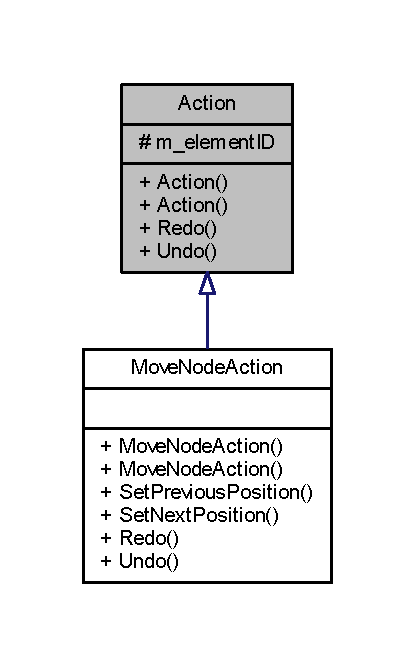
\includegraphics[width=199pt]{class_action__inherit__graph}
\end{center}
\end{figure}


Collaboration diagram for Action\+:\nopagebreak
\begin{figure}[H]
\begin{center}
\leavevmode
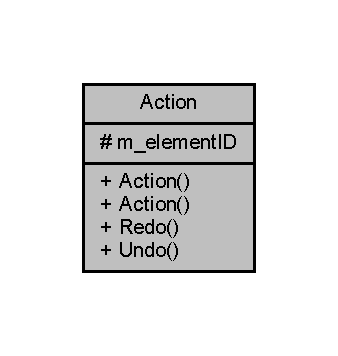
\includegraphics[width=162pt]{class_action__coll__graph}
\end{center}
\end{figure}
\subsection*{Public Member Functions}
\begin{DoxyCompactItemize}
\item 
\hyperlink{class_action_a4f457ccfc8336b565cadca56b36e0271}{Action} ()
\item 
\hyperlink{class_action_ab361b73e8653f33eee6b13b76d77bc62}{Action} (\hyperlink{_graphical_element_8h_ade5fd6c85839a416577ff9de1605141e}{Element\+Key} id)
\item 
virtual void \hyperlink{class_action_a69864cea344385ee84a5120eaab5d82a}{Redo} ()=0
\item 
virtual void \hyperlink{class_action_aab28a6693a01e51712ccbf4d24b6015e}{Undo} ()=0
\end{DoxyCompactItemize}
\subsection*{Protected Attributes}
\begin{DoxyCompactItemize}
\item 
\hyperlink{_graphical_element_8h_ade5fd6c85839a416577ff9de1605141e}{Element\+Key} \hyperlink{class_action_aa7b19bcb67e58c39675df7204d593b89}{m\+\_\+element\+ID}
\end{DoxyCompactItemize}
\subsection*{Friends}
\begin{DoxyCompactItemize}
\item 
class \hyperlink{class_action_a12790c6b4f2fb95ff77fbfec4dd07867}{History}
\end{DoxyCompactItemize}


\subsection{Detailed Description}


Definition at line 13 of file Action.\+h.



\subsection{Constructor \& Destructor Documentation}
\mbox{\Hypertarget{class_action_a4f457ccfc8336b565cadca56b36e0271}\label{class_action_a4f457ccfc8336b565cadca56b36e0271}} 
\index{Action@{Action}!Action@{Action}}
\index{Action@{Action}!Action@{Action}}
\subsubsection{\texorpdfstring{Action()}{Action()}\hspace{0.1cm}{\footnotesize\ttfamily [1/2]}}
{\footnotesize\ttfamily Action\+::\+Action (\begin{DoxyParamCaption}{ }\end{DoxyParamCaption})}



Definition at line 5 of file Action.\+cpp.

\mbox{\Hypertarget{class_action_ab361b73e8653f33eee6b13b76d77bc62}\label{class_action_ab361b73e8653f33eee6b13b76d77bc62}} 
\index{Action@{Action}!Action@{Action}}
\index{Action@{Action}!Action@{Action}}
\subsubsection{\texorpdfstring{Action()}{Action()}\hspace{0.1cm}{\footnotesize\ttfamily [2/2]}}
{\footnotesize\ttfamily Action\+::\+Action (\begin{DoxyParamCaption}\item[{\hyperlink{_graphical_element_8h_ade5fd6c85839a416577ff9de1605141e}{Element\+Key}}]{id }\end{DoxyParamCaption})}



Definition at line 7 of file Action.\+cpp.



\subsection{Member Function Documentation}
\mbox{\Hypertarget{class_action_a69864cea344385ee84a5120eaab5d82a}\label{class_action_a69864cea344385ee84a5120eaab5d82a}} 
\index{Action@{Action}!Redo@{Redo}}
\index{Redo@{Redo}!Action@{Action}}
\subsubsection{\texorpdfstring{Redo()}{Redo()}}
{\footnotesize\ttfamily virtual void Action\+::\+Redo (\begin{DoxyParamCaption}{ }\end{DoxyParamCaption})\hspace{0.3cm}{\ttfamily [pure virtual]}}



Implemented in \hyperlink{class_move_node_action_ae73d7a16920641dcc5b83f671e287223}{Move\+Node\+Action}.

Here is the caller graph for this function\+:
\nopagebreak
\begin{figure}[H]
\begin{center}
\leavevmode
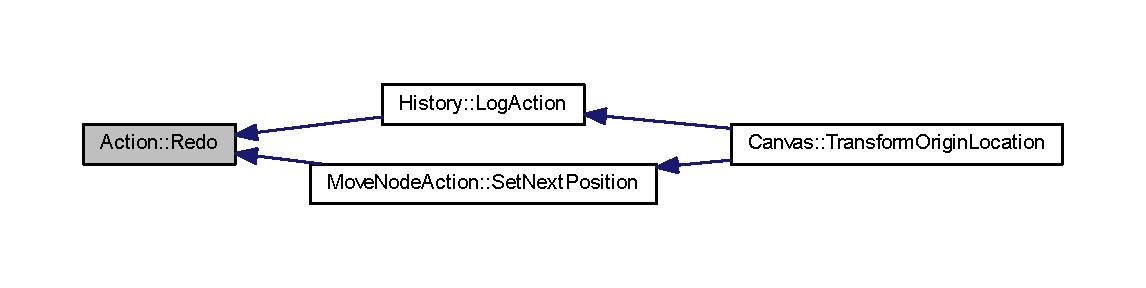
\includegraphics[width=350pt]{class_action_a69864cea344385ee84a5120eaab5d82a_icgraph}
\end{center}
\end{figure}
\mbox{\Hypertarget{class_action_aab28a6693a01e51712ccbf4d24b6015e}\label{class_action_aab28a6693a01e51712ccbf4d24b6015e}} 
\index{Action@{Action}!Undo@{Undo}}
\index{Undo@{Undo}!Action@{Action}}
\subsubsection{\texorpdfstring{Undo()}{Undo()}}
{\footnotesize\ttfamily virtual void Action\+::\+Undo (\begin{DoxyParamCaption}{ }\end{DoxyParamCaption})\hspace{0.3cm}{\ttfamily [pure virtual]}}



Implemented in \hyperlink{class_move_node_action_ad2136c2037da52ba1417c0c44b28d579}{Move\+Node\+Action}.

Here is the caller graph for this function\+:
\nopagebreak
\begin{figure}[H]
\begin{center}
\leavevmode
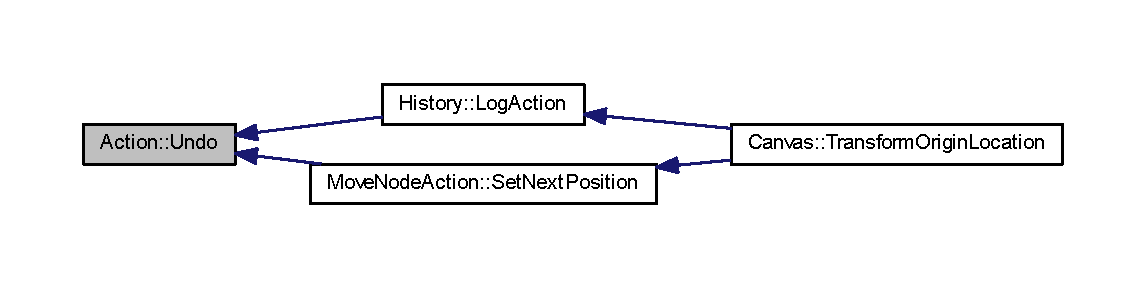
\includegraphics[width=350pt]{class_action_aab28a6693a01e51712ccbf4d24b6015e_icgraph}
\end{center}
\end{figure}


\subsection{Friends And Related Function Documentation}
\mbox{\Hypertarget{class_action_a12790c6b4f2fb95ff77fbfec4dd07867}\label{class_action_a12790c6b4f2fb95ff77fbfec4dd07867}} 
\index{Action@{Action}!History@{History}}
\index{History@{History}!Action@{Action}}
\subsubsection{\texorpdfstring{History}{History}}
{\footnotesize\ttfamily friend class \hyperlink{class_history}{History}\hspace{0.3cm}{\ttfamily [friend]}}



Definition at line 15 of file Action.\+h.



\subsection{Member Data Documentation}
\mbox{\Hypertarget{class_action_aa7b19bcb67e58c39675df7204d593b89}\label{class_action_aa7b19bcb67e58c39675df7204d593b89}} 
\index{Action@{Action}!m\+\_\+element\+ID@{m\+\_\+element\+ID}}
\index{m\+\_\+element\+ID@{m\+\_\+element\+ID}!Action@{Action}}
\subsubsection{\texorpdfstring{m\+\_\+element\+ID}{m\_elementID}}
{\footnotesize\ttfamily \hyperlink{_graphical_element_8h_ade5fd6c85839a416577ff9de1605141e}{Element\+Key} Action\+::m\+\_\+element\+ID\hspace{0.3cm}{\ttfamily [protected]}}



Definition at line 18 of file Action.\+h.



The documentation for this class was generated from the following files\+:\begin{DoxyCompactItemize}
\item 
Simulation Software/\+Source Files/\hyperlink{_action_8h}{Action.\+h}\item 
Simulation Software/\+Source Files/\hyperlink{_action_8cpp}{Action.\+cpp}\end{DoxyCompactItemize}

\hypertarget{class_source_node_1_1_arrive_e_a}{}\section{Source\+Node\+:\+:Arrive\+EA Class Reference}
\label{class_source_node_1_1_arrive_e_a}\index{Source\+Node\+::\+Arrive\+EA@{Source\+Node\+::\+Arrive\+EA}}


Inheritance diagram for Source\+Node\+:\+:Arrive\+EA\+:
\nopagebreak
\begin{figure}[H]
\begin{center}
\leavevmode
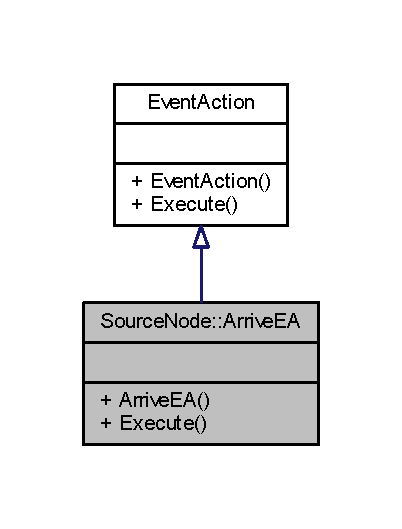
\includegraphics[width=193pt]{class_source_node_1_1_arrive_e_a__inherit__graph}
\end{center}
\end{figure}


Collaboration diagram for Source\+Node\+:\+:Arrive\+EA\+:
\nopagebreak
\begin{figure}[H]
\begin{center}
\leavevmode
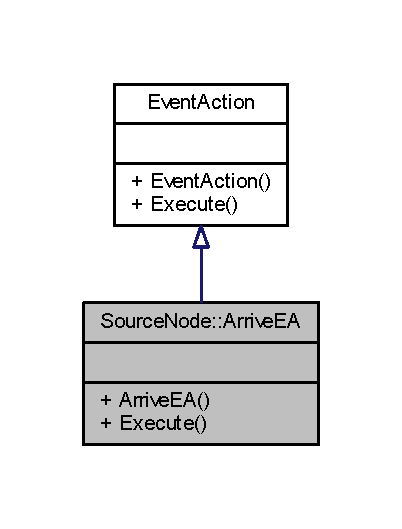
\includegraphics[width=193pt]{class_source_node_1_1_arrive_e_a__coll__graph}
\end{center}
\end{figure}
\subsection*{Public Member Functions}
\begin{DoxyCompactItemize}
\item 
\hyperlink{class_source_node_1_1_arrive_e_a_a6f956c34a412bb62b957b652cef8b19a}{Arrive\+EA} (\hyperlink{class_source_node}{Source\+Node} $\ast$src)
\item 
void \hyperlink{class_source_node_1_1_arrive_e_a_a622b2282aae023818b26d39519143c15}{Execute} ()
\end{DoxyCompactItemize}


\subsection{Detailed Description}


Definition at line 68 of file Specific\+Nodes.\+cpp.



\subsection{Constructor \& Destructor Documentation}
\mbox{\Hypertarget{class_source_node_1_1_arrive_e_a_a6f956c34a412bb62b957b652cef8b19a}\label{class_source_node_1_1_arrive_e_a_a6f956c34a412bb62b957b652cef8b19a}} 
\index{Source\+Node\+::\+Arrive\+EA@{Source\+Node\+::\+Arrive\+EA}!Arrive\+EA@{Arrive\+EA}}
\index{Arrive\+EA@{Arrive\+EA}!Source\+Node\+::\+Arrive\+EA@{Source\+Node\+::\+Arrive\+EA}}
\subsubsection{\texorpdfstring{Arrive\+E\+A()}{ArriveEA()}}
{\footnotesize\ttfamily Source\+Node\+::\+Arrive\+E\+A\+::\+Arrive\+EA (\begin{DoxyParamCaption}\item[{\hyperlink{class_source_node}{Source\+Node} $\ast$}]{src }\end{DoxyParamCaption})\hspace{0.3cm}{\ttfamily [inline]}}



Definition at line 71 of file Specific\+Nodes.\+cpp.



\subsection{Member Function Documentation}
\mbox{\Hypertarget{class_source_node_1_1_arrive_e_a_a622b2282aae023818b26d39519143c15}\label{class_source_node_1_1_arrive_e_a_a622b2282aae023818b26d39519143c15}} 
\index{Source\+Node\+::\+Arrive\+EA@{Source\+Node\+::\+Arrive\+EA}!Execute@{Execute}}
\index{Execute@{Execute}!Source\+Node\+::\+Arrive\+EA@{Source\+Node\+::\+Arrive\+EA}}
\subsubsection{\texorpdfstring{Execute()}{Execute()}}
{\footnotesize\ttfamily void Source\+Node\+::\+Arrive\+E\+A\+::\+Execute (\begin{DoxyParamCaption}{ }\end{DoxyParamCaption})\hspace{0.3cm}{\ttfamily [inline]}, {\ttfamily [virtual]}}



Implements \hyperlink{class_event_action_a62b9d07abb4ca8e7c078b076a1ab1a9f}{Event\+Action}.



Definition at line 75 of file Specific\+Nodes.\+cpp.

Here is the call graph for this function\+:
\nopagebreak
\begin{figure}[H]
\begin{center}
\leavevmode
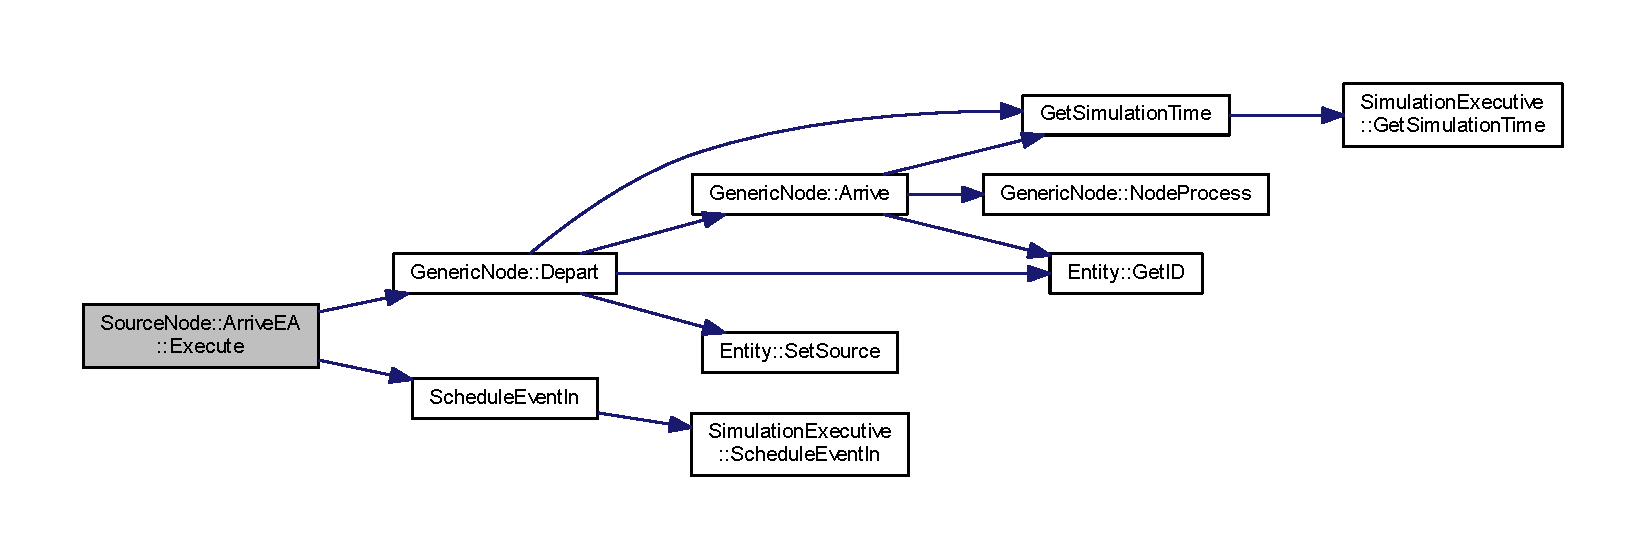
\includegraphics[width=350pt]{class_source_node_1_1_arrive_e_a_a622b2282aae023818b26d39519143c15_cgraph}
\end{center}
\end{figure}


The documentation for this class was generated from the following file\+:\begin{DoxyCompactItemize}
\item 
Simulation Software/\+Source Files/\hyperlink{_specific_nodes_8cpp}{Specific\+Nodes.\+cpp}\end{DoxyCompactItemize}

\hypertarget{class_canvas}{}\section{Canvas Class Reference}
\label{class_canvas}\index{Canvas@{Canvas}}


{\ttfamily \#include $<$Canvas.\+h$>$}



Inheritance diagram for Canvas\+:
\nopagebreak
\begin{figure}[H]
\begin{center}
\leavevmode
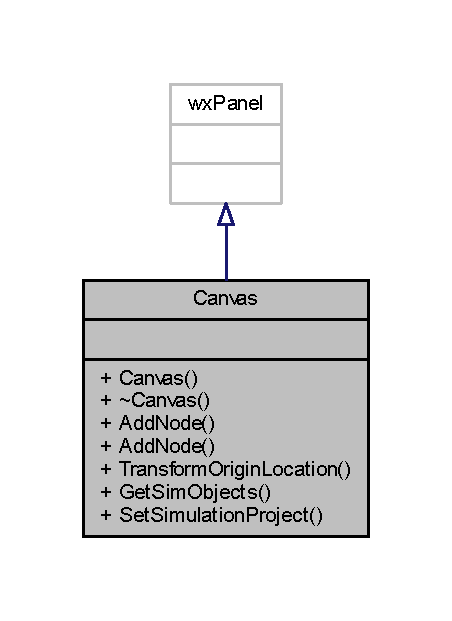
\includegraphics[width=217pt]{class_canvas__inherit__graph}
\end{center}
\end{figure}


Collaboration diagram for Canvas\+:
\nopagebreak
\begin{figure}[H]
\begin{center}
\leavevmode
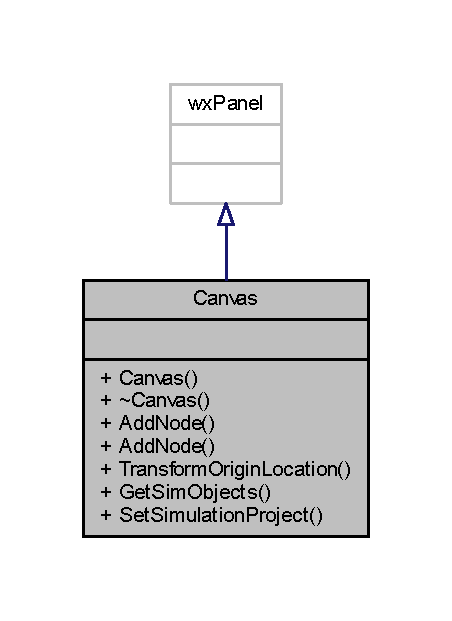
\includegraphics[width=217pt]{class_canvas__coll__graph}
\end{center}
\end{figure}
\subsection*{Public Member Functions}
\begin{DoxyCompactItemize}
\item 
\hyperlink{class_canvas_ae31d296f6d7a0d3a2958ca1d7e61a51d}{Canvas} (wx\+Window $\ast$parent, wx\+Status\+Bar $\ast$status)
\item 
\hyperlink{class_canvas_a237c4549ad2e27c729cd1f71e89f0fd9}{$\sim$\+Canvas} ()
\item 
void \hyperlink{class_canvas_aec9038762b17b62ff6126bd6277a9cd8}{Add\+Node} (\hyperlink{class_generic_node_a9e7985ab9bbfa1c85091adc0ab71a6b6}{Generic\+Node\+::\+Type} type, wx\+Point2\+D\+Double center, const std\+::string \&label)
\item 
void \hyperlink{class_canvas_aaec53b68c7b24704e399b565731ed545}{Add\+Node} (\hyperlink{class_generic_node_a9e7985ab9bbfa1c85091adc0ab71a6b6}{Generic\+Node\+::\+Type} type, wx\+Point2\+D\+Double center)
\item 
void \hyperlink{class_canvas_a4afa0e24da7b82be3696131c13d89404}{Transform\+Origin\+Location} (wx\+Size canvas\+Size)
\item 
\hyperlink{class_set}{Set}$<$ \hyperlink{class_graphical_node}{Graphical\+Node} $>$ \hyperlink{class_canvas_a21d8ffb18a14cb10af590d3d66efe956}{Get\+Sim\+Objects} ()
\item 
void \hyperlink{class_canvas_ae7b17a82b7376ee4105b8f36179ab90e}{Set\+Simulation\+Project} (\hyperlink{class_sim_project}{Sim\+Project} $\ast$parent\+Project)
\end{DoxyCompactItemize}


\subsection{Detailed Description}


Definition at line 14 of file Canvas.\+h.



\subsection{Constructor \& Destructor Documentation}
\mbox{\Hypertarget{class_canvas_ae31d296f6d7a0d3a2958ca1d7e61a51d}\label{class_canvas_ae31d296f6d7a0d3a2958ca1d7e61a51d}} 
\index{Canvas@{Canvas}!Canvas@{Canvas}}
\index{Canvas@{Canvas}!Canvas@{Canvas}}
\subsubsection{\texorpdfstring{Canvas()}{Canvas()}}
{\footnotesize\ttfamily Canvas\+::\+Canvas (\begin{DoxyParamCaption}\item[{wx\+Window $\ast$}]{parent,  }\item[{wx\+Status\+Bar $\ast$}]{status }\end{DoxyParamCaption})}



Definition at line 8 of file Canvas.\+cpp.

\mbox{\Hypertarget{class_canvas_a237c4549ad2e27c729cd1f71e89f0fd9}\label{class_canvas_a237c4549ad2e27c729cd1f71e89f0fd9}} 
\index{Canvas@{Canvas}!````~Canvas@{$\sim$\+Canvas}}
\index{````~Canvas@{$\sim$\+Canvas}!Canvas@{Canvas}}
\subsubsection{\texorpdfstring{$\sim$\+Canvas()}{~Canvas()}}
{\footnotesize\ttfamily Canvas\+::$\sim$\+Canvas (\begin{DoxyParamCaption}{ }\end{DoxyParamCaption})}



Definition at line 63 of file Canvas.\+cpp.

Here is the call graph for this function\+:
\nopagebreak
\begin{figure}[H]
\begin{center}
\leavevmode
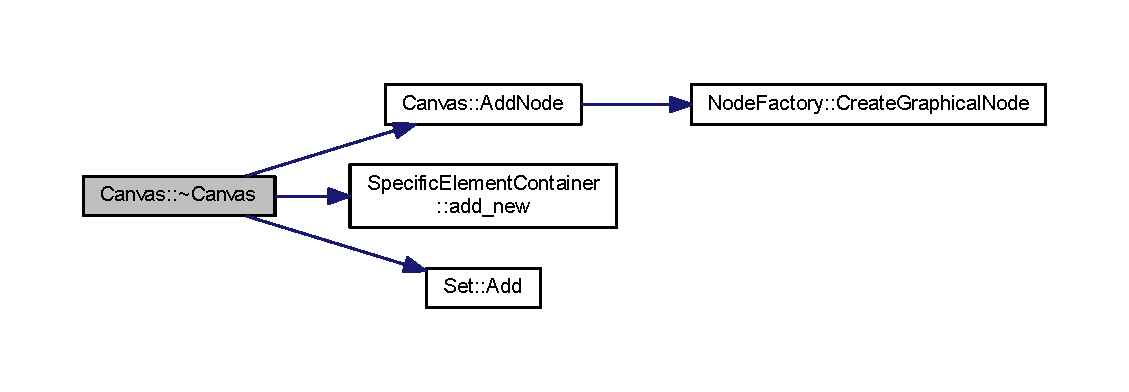
\includegraphics[width=350pt]{class_canvas_a237c4549ad2e27c729cd1f71e89f0fd9_cgraph}
\end{center}
\end{figure}


\subsection{Member Function Documentation}
\mbox{\Hypertarget{class_canvas_aec9038762b17b62ff6126bd6277a9cd8}\label{class_canvas_aec9038762b17b62ff6126bd6277a9cd8}} 
\index{Canvas@{Canvas}!Add\+Node@{Add\+Node}}
\index{Add\+Node@{Add\+Node}!Canvas@{Canvas}}
\subsubsection{\texorpdfstring{Add\+Node()}{AddNode()}\hspace{0.1cm}{\footnotesize\ttfamily [1/2]}}
{\footnotesize\ttfamily void Canvas\+::\+Add\+Node (\begin{DoxyParamCaption}\item[{\hyperlink{class_generic_node_a9e7985ab9bbfa1c85091adc0ab71a6b6}{Generic\+Node\+::\+Type}}]{type,  }\item[{wx\+Point2\+D\+Double}]{center,  }\item[{const std\+::string \&}]{label }\end{DoxyParamCaption})}



Definition at line 77 of file Canvas.\+cpp.

Here is the call graph for this function\+:
\nopagebreak
\begin{figure}[H]
\begin{center}
\leavevmode
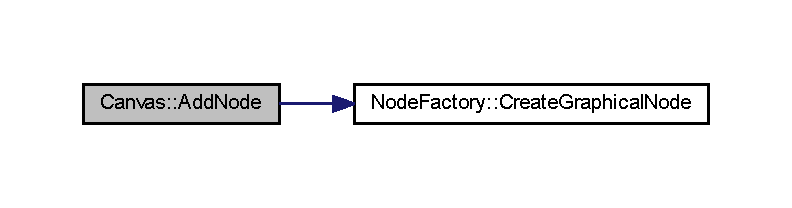
\includegraphics[width=350pt]{class_canvas_aec9038762b17b62ff6126bd6277a9cd8_cgraph}
\end{center}
\end{figure}
Here is the caller graph for this function\+:
\nopagebreak
\begin{figure}[H]
\begin{center}
\leavevmode
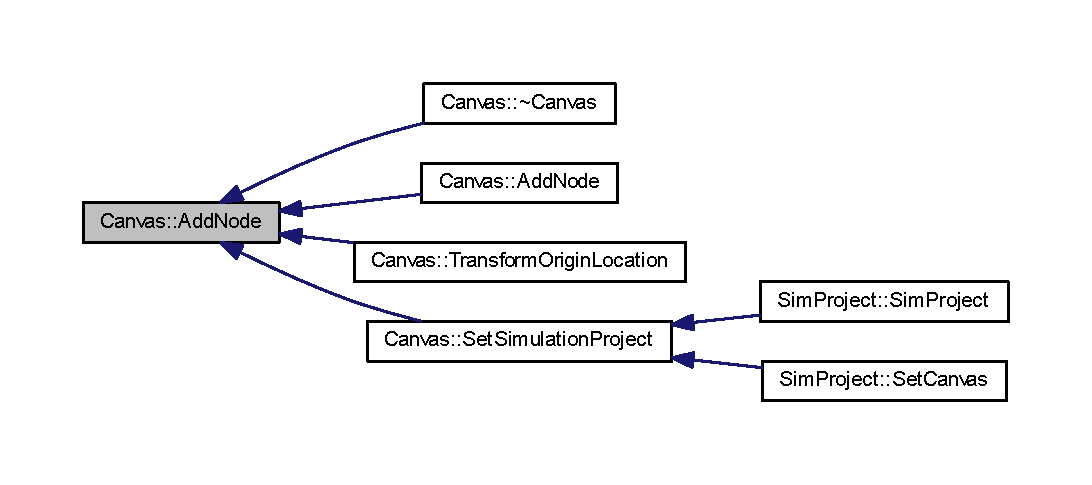
\includegraphics[width=350pt]{class_canvas_aec9038762b17b62ff6126bd6277a9cd8_icgraph}
\end{center}
\end{figure}
\mbox{\Hypertarget{class_canvas_aaec53b68c7b24704e399b565731ed545}\label{class_canvas_aaec53b68c7b24704e399b565731ed545}} 
\index{Canvas@{Canvas}!Add\+Node@{Add\+Node}}
\index{Add\+Node@{Add\+Node}!Canvas@{Canvas}}
\subsubsection{\texorpdfstring{Add\+Node()}{AddNode()}\hspace{0.1cm}{\footnotesize\ttfamily [2/2]}}
{\footnotesize\ttfamily void Canvas\+::\+Add\+Node (\begin{DoxyParamCaption}\item[{\hyperlink{class_generic_node_a9e7985ab9bbfa1c85091adc0ab71a6b6}{Generic\+Node\+::\+Type}}]{type,  }\item[{wx\+Point2\+D\+Double}]{center }\end{DoxyParamCaption})}



Definition at line 89 of file Canvas.\+cpp.

Here is the call graph for this function\+:
\nopagebreak
\begin{figure}[H]
\begin{center}
\leavevmode
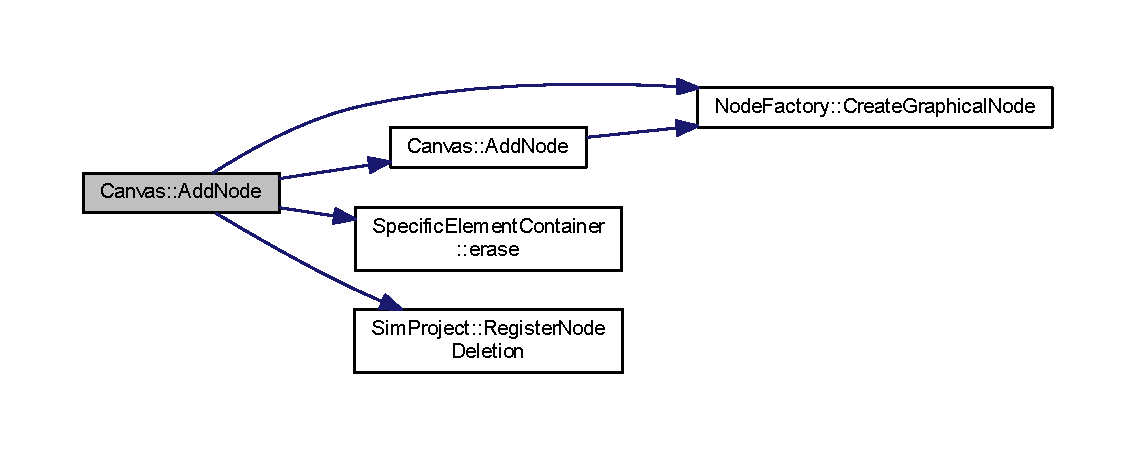
\includegraphics[width=350pt]{class_canvas_aaec53b68c7b24704e399b565731ed545_cgraph}
\end{center}
\end{figure}
\mbox{\Hypertarget{class_canvas_a21d8ffb18a14cb10af590d3d66efe956}\label{class_canvas_a21d8ffb18a14cb10af590d3d66efe956}} 
\index{Canvas@{Canvas}!Get\+Sim\+Objects@{Get\+Sim\+Objects}}
\index{Get\+Sim\+Objects@{Get\+Sim\+Objects}!Canvas@{Canvas}}
\subsubsection{\texorpdfstring{Get\+Sim\+Objects()}{GetSimObjects()}}
{\footnotesize\ttfamily \hyperlink{class_set}{Set}$<$ \hyperlink{class_graphical_node}{Graphical\+Node} $>$ Canvas\+::\+Get\+Sim\+Objects (\begin{DoxyParamCaption}{ }\end{DoxyParamCaption})}



Definition at line 166 of file Canvas.\+cpp.

Here is the caller graph for this function\+:
\nopagebreak
\begin{figure}[H]
\begin{center}
\leavevmode
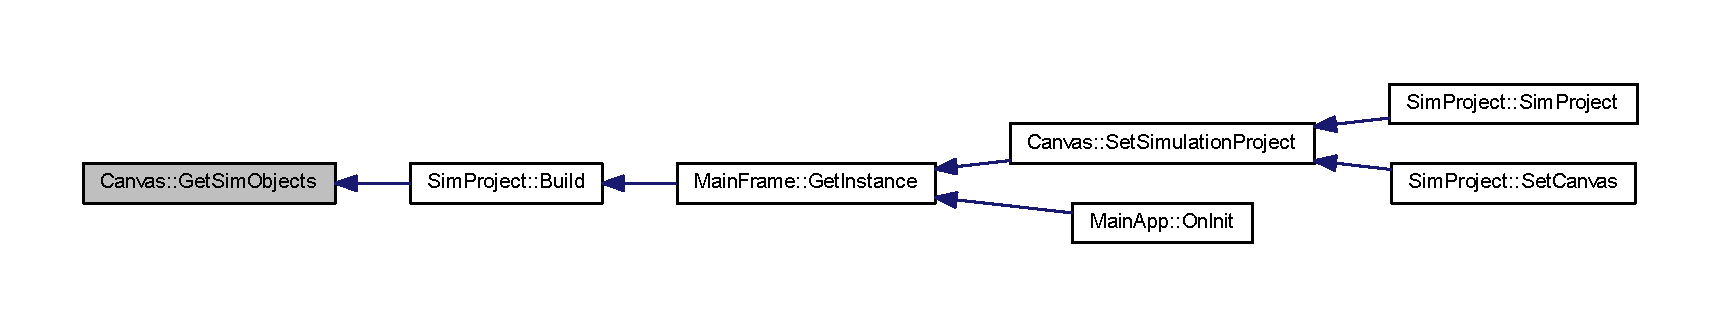
\includegraphics[width=350pt]{class_canvas_a21d8ffb18a14cb10af590d3d66efe956_icgraph}
\end{center}
\end{figure}
\mbox{\Hypertarget{class_canvas_ae7b17a82b7376ee4105b8f36179ab90e}\label{class_canvas_ae7b17a82b7376ee4105b8f36179ab90e}} 
\index{Canvas@{Canvas}!Set\+Simulation\+Project@{Set\+Simulation\+Project}}
\index{Set\+Simulation\+Project@{Set\+Simulation\+Project}!Canvas@{Canvas}}
\subsubsection{\texorpdfstring{Set\+Simulation\+Project()}{SetSimulationProject()}}
{\footnotesize\ttfamily void Canvas\+::\+Set\+Simulation\+Project (\begin{DoxyParamCaption}\item[{\hyperlink{class_sim_project}{Sim\+Project} $\ast$}]{parent\+Project }\end{DoxyParamCaption})}



Definition at line 171 of file Canvas.\+cpp.

Here is the call graph for this function\+:
\nopagebreak
\begin{figure}[H]
\begin{center}
\leavevmode
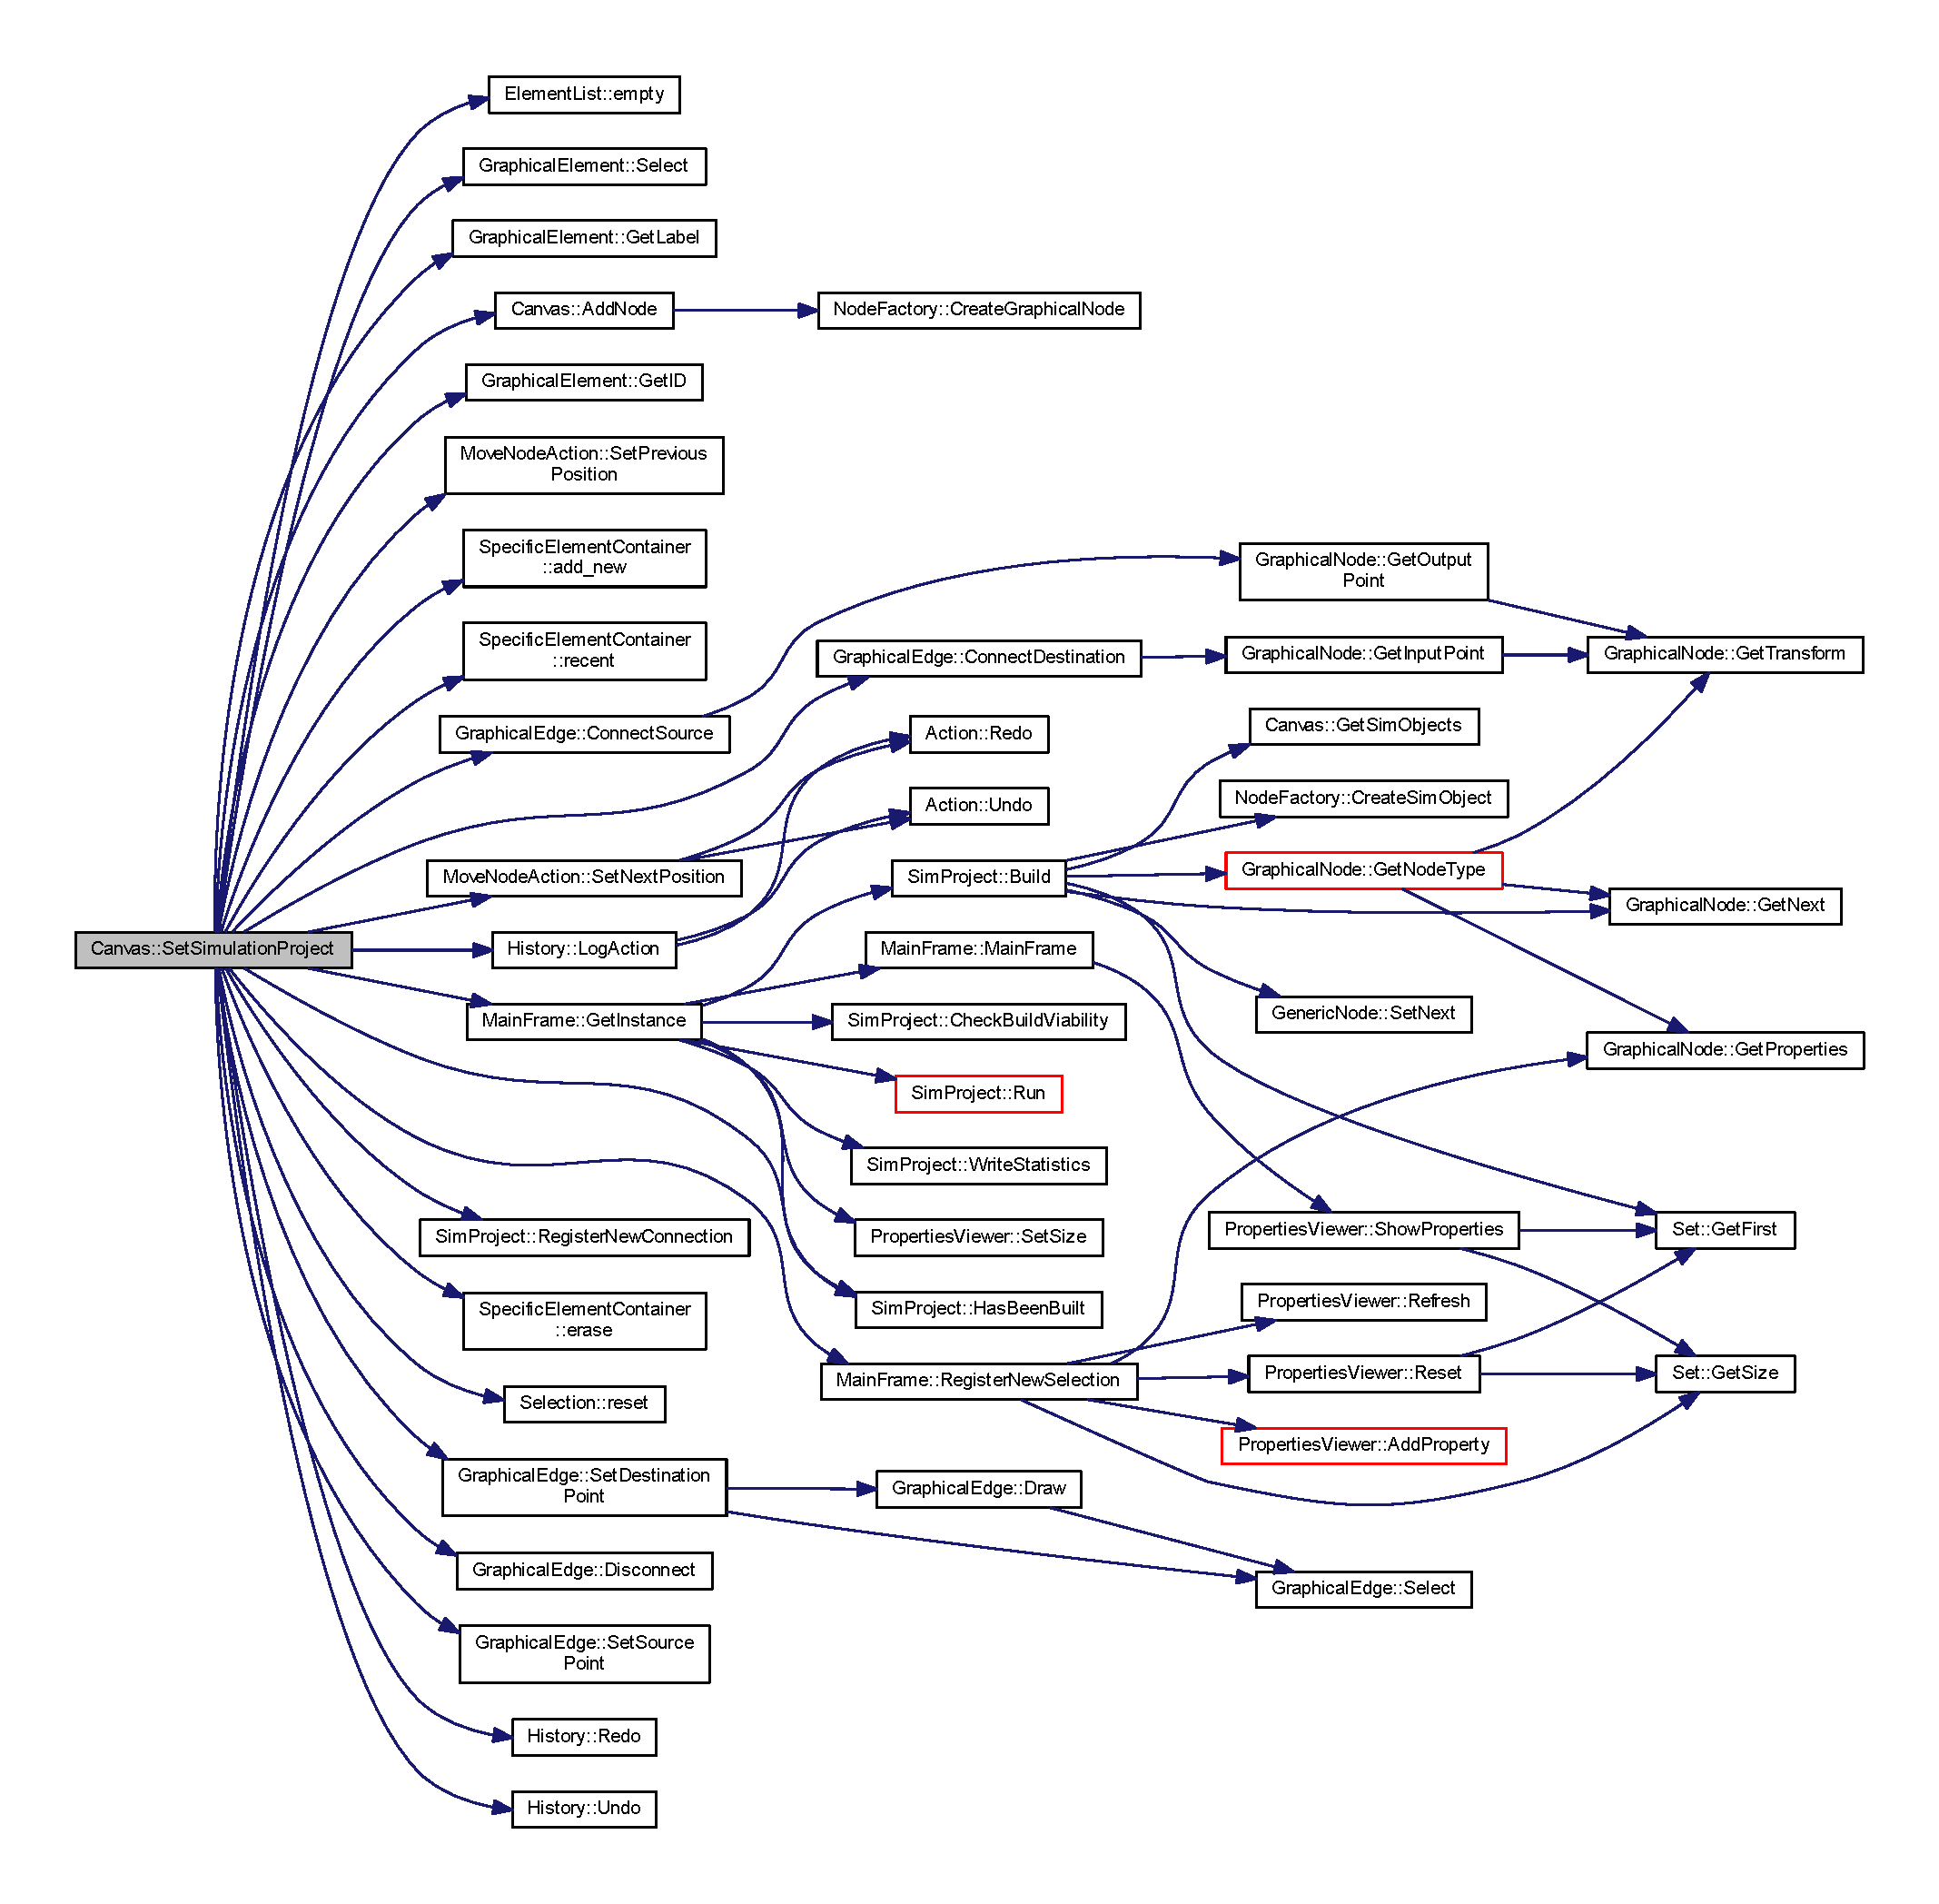
\includegraphics[width=350pt]{class_canvas_ae7b17a82b7376ee4105b8f36179ab90e_cgraph}
\end{center}
\end{figure}
Here is the caller graph for this function\+:
\nopagebreak
\begin{figure}[H]
\begin{center}
\leavevmode
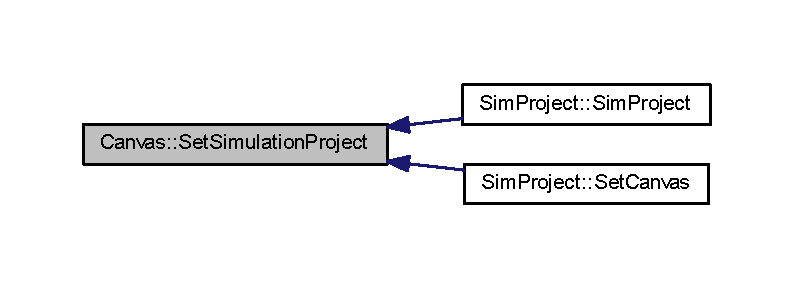
\includegraphics[width=350pt]{class_canvas_ae7b17a82b7376ee4105b8f36179ab90e_icgraph}
\end{center}
\end{figure}
\mbox{\Hypertarget{class_canvas_a4afa0e24da7b82be3696131c13d89404}\label{class_canvas_a4afa0e24da7b82be3696131c13d89404}} 
\index{Canvas@{Canvas}!Transform\+Origin\+Location@{Transform\+Origin\+Location}}
\index{Transform\+Origin\+Location@{Transform\+Origin\+Location}!Canvas@{Canvas}}
\subsubsection{\texorpdfstring{Transform\+Origin\+Location()}{TransformOriginLocation()}}
{\footnotesize\ttfamily void Canvas\+::\+Transform\+Origin\+Location (\begin{DoxyParamCaption}\item[{wx\+Size}]{canvas\+Size }\end{DoxyParamCaption})}



Definition at line 145 of file Canvas.\+cpp.

Here is the call graph for this function\+:
\nopagebreak
\begin{figure}[H]
\begin{center}
\leavevmode
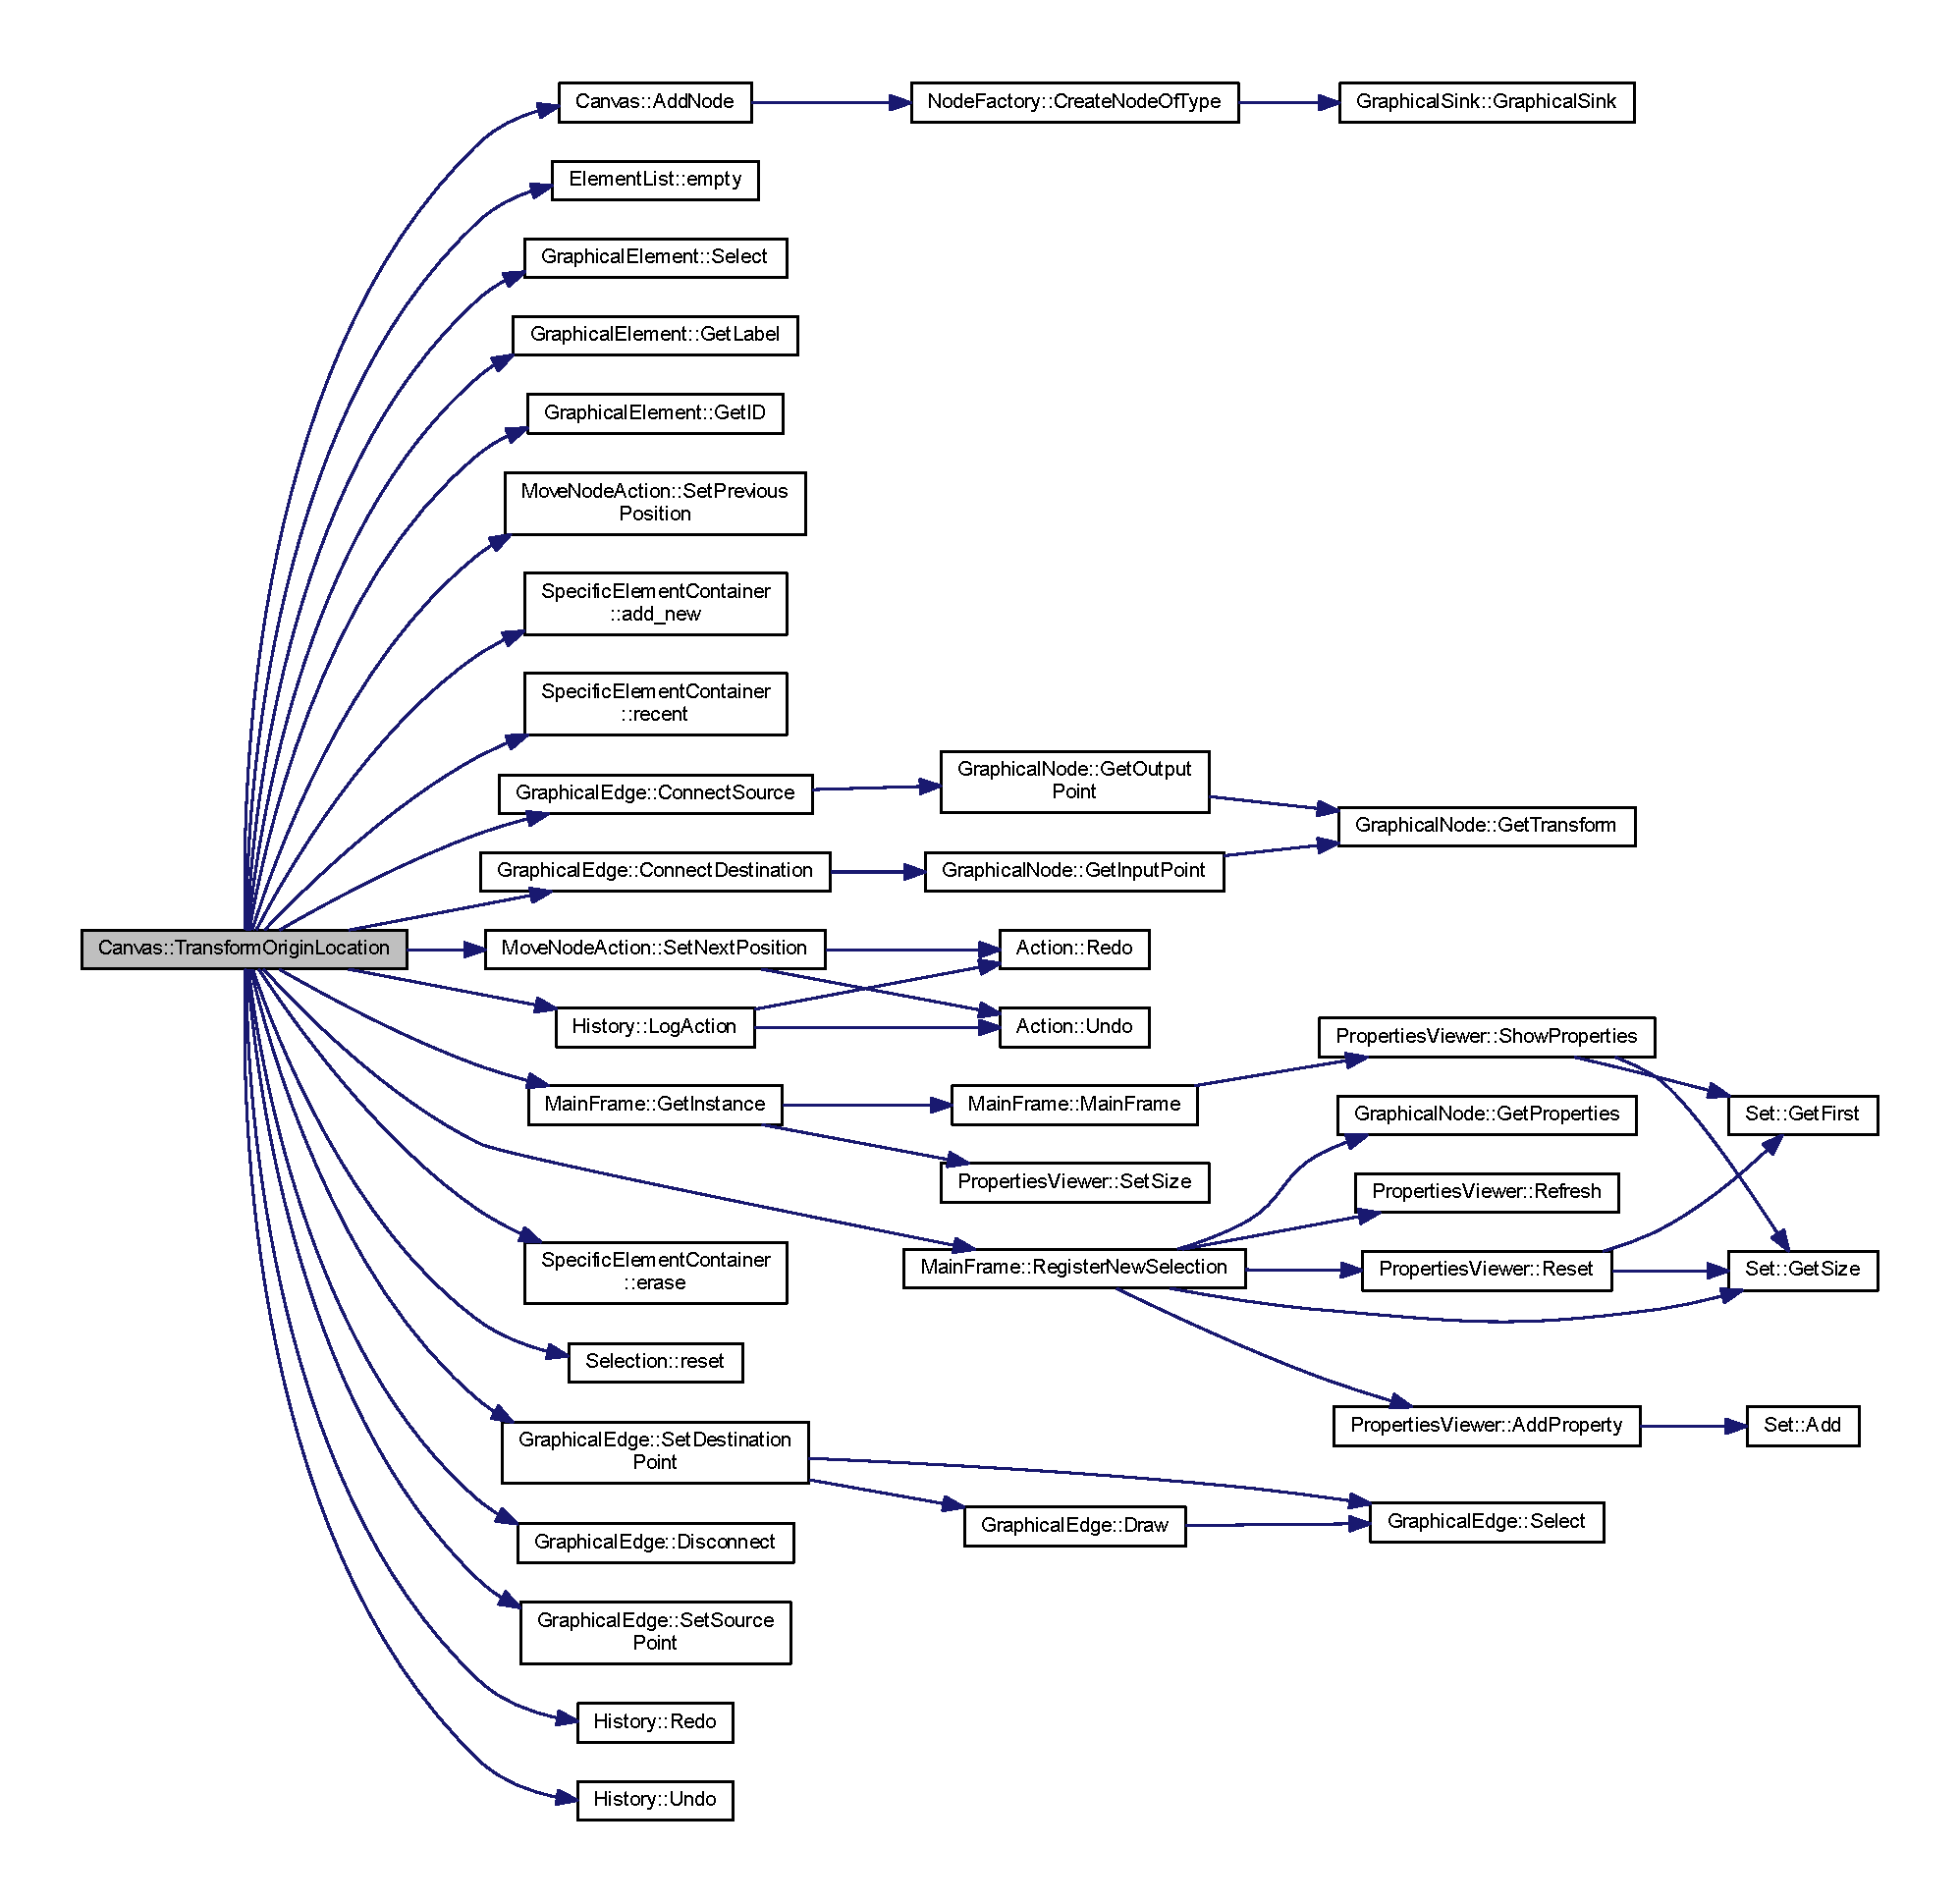
\includegraphics[width=350pt]{class_canvas_a4afa0e24da7b82be3696131c13d89404_cgraph}
\end{center}
\end{figure}


The documentation for this class was generated from the following files\+:\begin{DoxyCompactItemize}
\item 
Simulation Software/\+Source Files/\hyperlink{_canvas_8h}{Canvas.\+h}\item 
Simulation Software/\+Source Files/\hyperlink{_canvas_8cpp}{Canvas.\+cpp}\end{DoxyCompactItemize}

\hypertarget{class_connection}{}\section{Connection Class Reference}
\label{class_connection}\index{Connection@{Connection}}


{\ttfamily \#include $<$Generic\+Node.\+h$>$}



Inheritance diagram for Connection\+:
\nopagebreak
\begin{figure}[H]
\begin{center}
\leavevmode
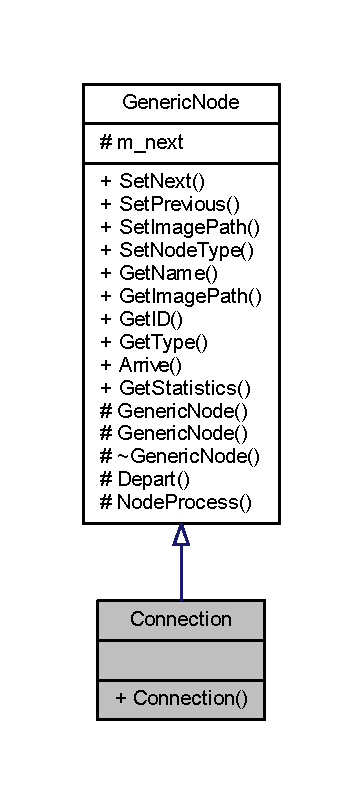
\includegraphics[width=174pt]{class_connection__inherit__graph}
\end{center}
\end{figure}


Collaboration diagram for Connection\+:
\nopagebreak
\begin{figure}[H]
\begin{center}
\leavevmode
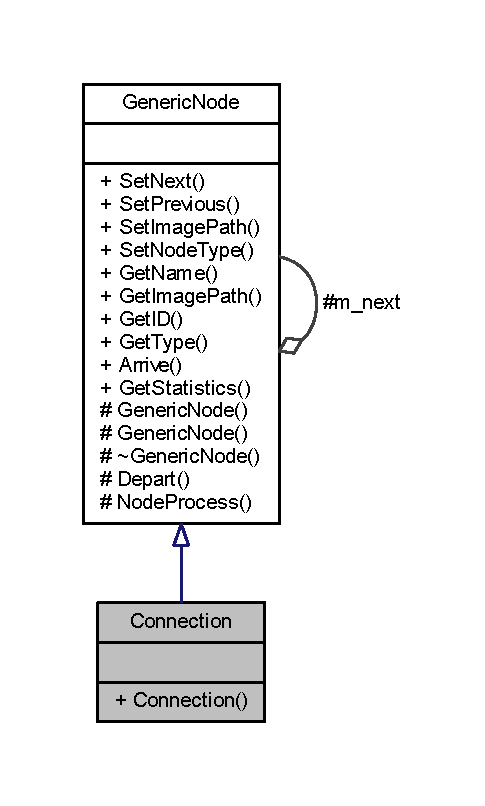
\includegraphics[width=233pt]{class_connection__coll__graph}
\end{center}
\end{figure}
\subsection*{Public Member Functions}
\begin{DoxyCompactItemize}
\item 
\hyperlink{class_connection_a9f0ec6c9f46d973813357248e2600695}{Connection} (\hyperlink{class_generic_node}{Generic\+Node} $\ast$start\+Block, \hyperlink{class_generic_node}{Generic\+Node} $\ast$end\+Block)
\end{DoxyCompactItemize}
\subsection*{Additional Inherited Members}


\subsection{Detailed Description}


Definition at line 78 of file Generic\+Node.\+h.



\subsection{Constructor \& Destructor Documentation}
\mbox{\Hypertarget{class_connection_a9f0ec6c9f46d973813357248e2600695}\label{class_connection_a9f0ec6c9f46d973813357248e2600695}} 
\index{Connection@{Connection}!Connection@{Connection}}
\index{Connection@{Connection}!Connection@{Connection}}
\subsubsection{\texorpdfstring{Connection()}{Connection()}}
{\footnotesize\ttfamily Connection\+::\+Connection (\begin{DoxyParamCaption}\item[{\hyperlink{class_generic_node}{Generic\+Node} $\ast$}]{start\+Block,  }\item[{\hyperlink{class_generic_node}{Generic\+Node} $\ast$}]{end\+Block }\end{DoxyParamCaption})\hspace{0.3cm}{\ttfamily [inline]}}



Definition at line 81 of file Generic\+Node.\+h.



The documentation for this class was generated from the following file\+:\begin{DoxyCompactItemize}
\item 
Simulation Software/\+Source Files/\hyperlink{_generic_node_8h}{Generic\+Node.\+h}\end{DoxyCompactItemize}

\hypertarget{class_constant}{}\section{Constant Class Reference}
\label{class_constant}\index{Constant@{Constant}}


{\ttfamily \#include $<$Distribution.\+h$>$}



Inheritance diagram for Constant\+:
\nopagebreak
\begin{figure}[H]
\begin{center}
\leavevmode
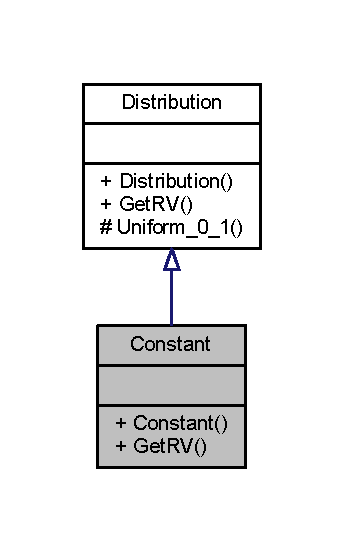
\includegraphics[width=165pt]{class_constant__inherit__graph}
\end{center}
\end{figure}


Collaboration diagram for Constant\+:
\nopagebreak
\begin{figure}[H]
\begin{center}
\leavevmode
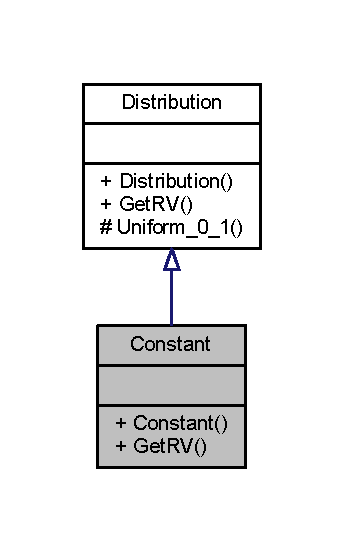
\includegraphics[width=165pt]{class_constant__coll__graph}
\end{center}
\end{figure}
\subsection*{Public Member Functions}
\begin{DoxyCompactItemize}
\item 
\hyperlink{class_constant_a9b181fdf7e935c56d3b58133ce21efb8}{Constant} (double mean)
\item 
double \hyperlink{class_constant_a9eac5a0bdc360c859f187f8aa94dcd6d}{Get\+RV} ()
\end{DoxyCompactItemize}
\subsection*{Additional Inherited Members}


\subsection{Detailed Description}


Definition at line 61 of file Distribution.\+h.



\subsection{Constructor \& Destructor Documentation}
\mbox{\Hypertarget{class_constant_a9b181fdf7e935c56d3b58133ce21efb8}\label{class_constant_a9b181fdf7e935c56d3b58133ce21efb8}} 
\index{Constant@{Constant}!Constant@{Constant}}
\index{Constant@{Constant}!Constant@{Constant}}
\subsubsection{\texorpdfstring{Constant()}{Constant()}}
{\footnotesize\ttfamily Constant\+::\+Constant (\begin{DoxyParamCaption}\item[{double}]{mean }\end{DoxyParamCaption})}



Definition at line 93 of file Distribution.\+cpp.



\subsection{Member Function Documentation}
\mbox{\Hypertarget{class_constant_a9eac5a0bdc360c859f187f8aa94dcd6d}\label{class_constant_a9eac5a0bdc360c859f187f8aa94dcd6d}} 
\index{Constant@{Constant}!Get\+RV@{Get\+RV}}
\index{Get\+RV@{Get\+RV}!Constant@{Constant}}
\subsubsection{\texorpdfstring{Get\+R\+V()}{GetRV()}}
{\footnotesize\ttfamily double Constant\+::\+Get\+RV (\begin{DoxyParamCaption}{ }\end{DoxyParamCaption})\hspace{0.3cm}{\ttfamily [virtual]}}



Implements \hyperlink{class_distribution_a63b433850d7b47d84eb69448f7916719}{Distribution}.



Definition at line 98 of file Distribution.\+cpp.



The documentation for this class was generated from the following files\+:\begin{DoxyCompactItemize}
\item 
Simulation Software/\+Source Files/\hyperlink{_distribution_8h}{Distribution.\+h}\item 
Simulation Software/\+Source Files/\hyperlink{_distribution_8cpp}{Distribution.\+cpp}\end{DoxyCompactItemize}

\hypertarget{class_distribution}{}\section{Distribution Class Reference}
\label{class_distribution}\index{Distribution@{Distribution}}


{\ttfamily \#include $<$Distribution.\+h$>$}



Inheritance diagram for Distribution\+:\nopagebreak
\begin{figure}[H]
\begin{center}
\leavevmode
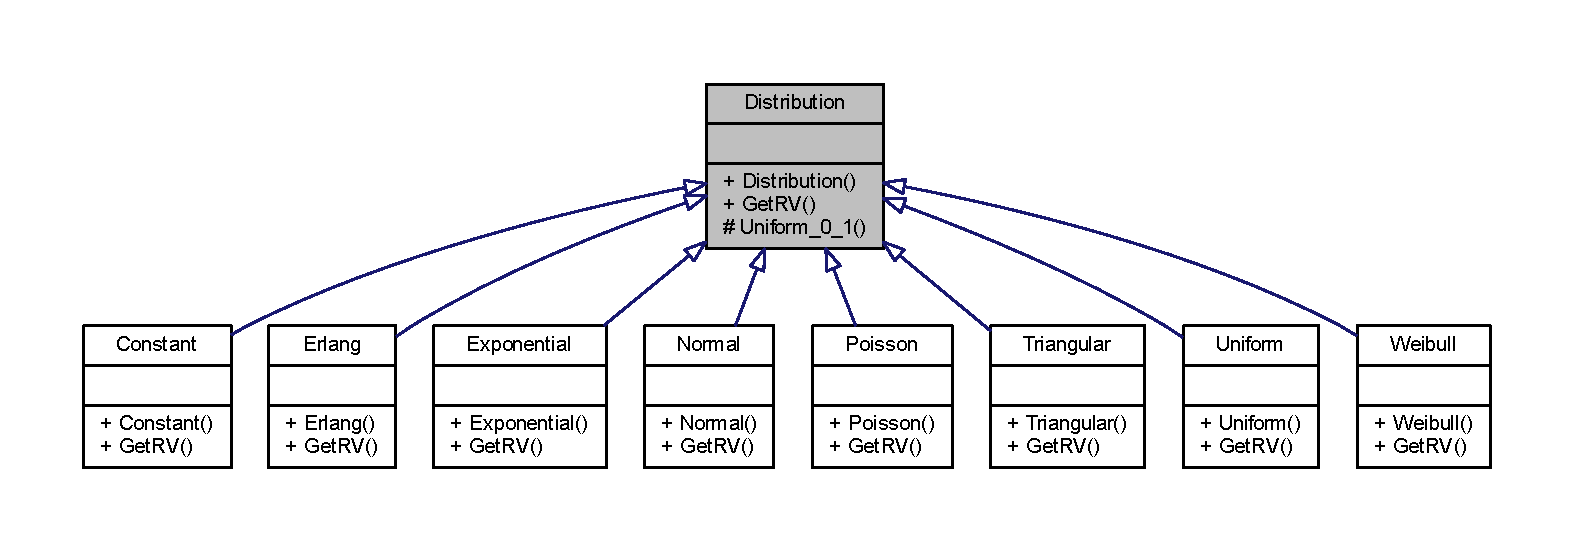
\includegraphics[width=350pt]{class_distribution__inherit__graph}
\end{center}
\end{figure}


Collaboration diagram for Distribution\+:\nopagebreak
\begin{figure}[H]
\begin{center}
\leavevmode
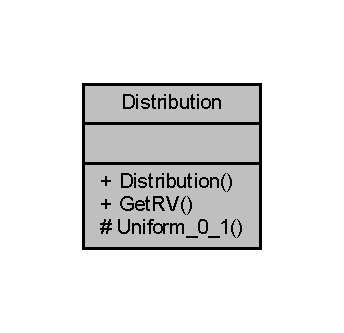
\includegraphics[width=165pt]{class_distribution__coll__graph}
\end{center}
\end{figure}
\subsection*{Public Member Functions}
\begin{DoxyCompactItemize}
\item 
\hyperlink{class_distribution_ada837c9a1da728290d6bbea0bb6b266f}{Distribution} ()
\item 
virtual double \hyperlink{class_distribution_a63b433850d7b47d84eb69448f7916719}{Get\+RV} ()=0
\end{DoxyCompactItemize}
\subsection*{Protected Member Functions}
\begin{DoxyCompactItemize}
\item 
double \hyperlink{class_distribution_a33965648e4c6d3bbc93c61ccd3897c98}{Uniform\+\_\+0\+\_\+1} ()
\end{DoxyCompactItemize}


\subsection{Detailed Description}


Definition at line 4 of file Distribution.\+h.



\subsection{Constructor \& Destructor Documentation}
\mbox{\Hypertarget{class_distribution_ada837c9a1da728290d6bbea0bb6b266f}\label{class_distribution_ada837c9a1da728290d6bbea0bb6b266f}} 
\index{Distribution@{Distribution}!Distribution@{Distribution}}
\index{Distribution@{Distribution}!Distribution@{Distribution}}
\subsubsection{\texorpdfstring{Distribution()}{Distribution()}}
{\footnotesize\ttfamily Distribution\+::\+Distribution (\begin{DoxyParamCaption}{ }\end{DoxyParamCaption})}



Definition at line 5 of file Distribution.\+cpp.



\subsection{Member Function Documentation}
\mbox{\Hypertarget{class_distribution_a63b433850d7b47d84eb69448f7916719}\label{class_distribution_a63b433850d7b47d84eb69448f7916719}} 
\index{Distribution@{Distribution}!Get\+RV@{Get\+RV}}
\index{Get\+RV@{Get\+RV}!Distribution@{Distribution}}
\subsubsection{\texorpdfstring{Get\+R\+V()}{GetRV()}}
{\footnotesize\ttfamily virtual double Distribution\+::\+Get\+RV (\begin{DoxyParamCaption}{ }\end{DoxyParamCaption})\hspace{0.3cm}{\ttfamily [pure virtual]}}



Implemented in \hyperlink{class_erlang_a5ae5b56e37bd2c5ee4318fcc12259442}{Erlang}, \hyperlink{class_weibull_a0de3910ff51aeb87c49ccb5d34d1de0d}{Weibull}, \hyperlink{class_constant_a9eac5a0bdc360c859f187f8aa94dcd6d}{Constant}, \hyperlink{class_poisson_a068964aa05df4051b23a84d71529fb69}{Poisson}, \hyperlink{class_normal_a6101d2303601a4f7dfa33fe4b104df7e}{Normal}, \hyperlink{class_triangular_aadd53c452801be8c0eb6ffb31a299835}{Triangular}, \hyperlink{class_uniform_a9350886d5ad1854294ecff338a288fc7}{Uniform}, and \hyperlink{class_exponential_a2a45aeaf0a3725174d86712761a8dd82}{Exponential}.

Here is the caller graph for this function\+:\nopagebreak
\begin{figure}[H]
\begin{center}
\leavevmode
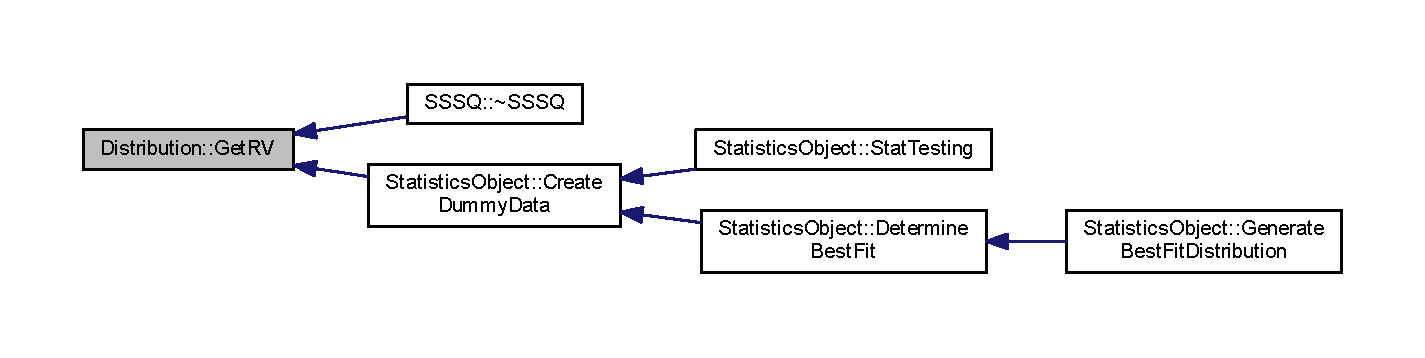
\includegraphics[width=350pt]{class_distribution_a63b433850d7b47d84eb69448f7916719_icgraph}
\end{center}
\end{figure}
\mbox{\Hypertarget{class_distribution_a33965648e4c6d3bbc93c61ccd3897c98}\label{class_distribution_a33965648e4c6d3bbc93c61ccd3897c98}} 
\index{Distribution@{Distribution}!Uniform\+\_\+0\+\_\+1@{Uniform\+\_\+0\+\_\+1}}
\index{Uniform\+\_\+0\+\_\+1@{Uniform\+\_\+0\+\_\+1}!Distribution@{Distribution}}
\subsubsection{\texorpdfstring{Uniform\+\_\+0\+\_\+1()}{Uniform\_0\_1()}}
{\footnotesize\ttfamily double Distribution\+::\+Uniform\+\_\+0\+\_\+1 (\begin{DoxyParamCaption}{ }\end{DoxyParamCaption})\hspace{0.3cm}{\ttfamily [protected]}}



Definition at line 7 of file Distribution.\+cpp.

Here is the caller graph for this function\+:\nopagebreak
\begin{figure}[H]
\begin{center}
\leavevmode
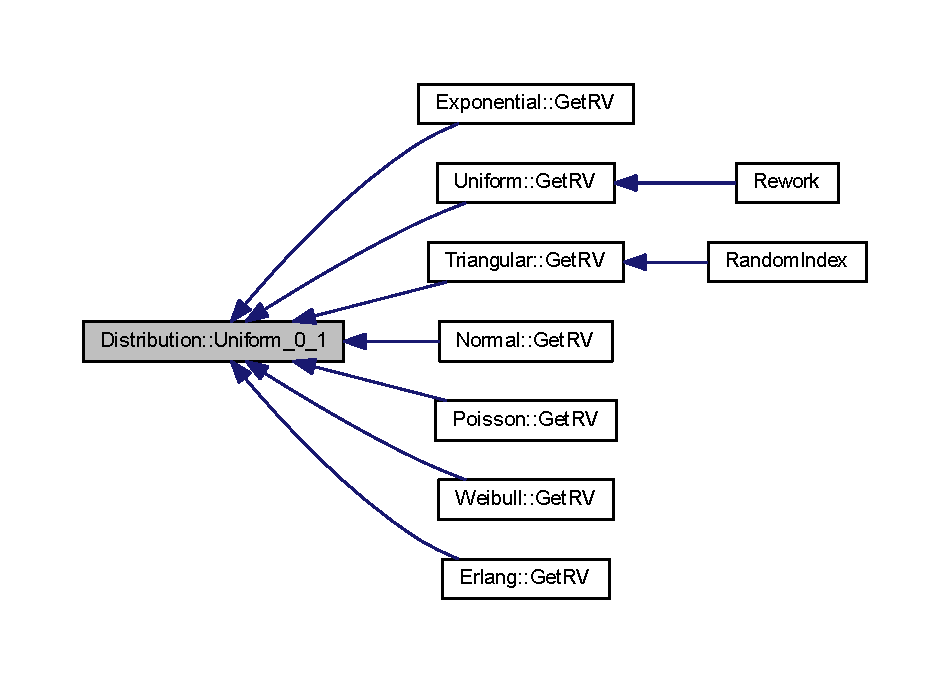
\includegraphics[width=350pt]{class_distribution_a33965648e4c6d3bbc93c61ccd3897c98_icgraph}
\end{center}
\end{figure}


The documentation for this class was generated from the following files\+:\begin{DoxyCompactItemize}
\item 
Simulation Software/\+Source Files/\hyperlink{_distribution_8h}{Distribution.\+h}\item 
Simulation Software/\+Source Files/\hyperlink{_distribution_8cpp}{Distribution.\+cpp}\end{DoxyCompactItemize}

\hypertarget{class_element_list}{}\section{Element\+List Class Reference}
\label{class_element_list}\index{Element\+List@{Element\+List}}


{\ttfamily \#include $<$Graphical\+Element.\+h$>$}



Collaboration diagram for Element\+List\+:\nopagebreak
\begin{figure}[H]
\begin{center}
\leavevmode
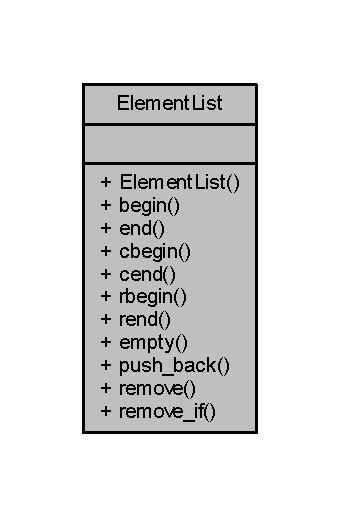
\includegraphics[width=163pt]{class_element_list__coll__graph}
\end{center}
\end{figure}
\subsection*{Public Types}
\begin{DoxyCompactItemize}
\item 
typedef List\+::iterator \hyperlink{class_element_list_a10e1b0c17ebe441fcd035fcf0a00d25e}{iterator}
\item 
typedef List\+::const\+\_\+iterator \hyperlink{class_element_list_a4323074a8e979322c0bf1eed5c892cf4}{const\+\_\+iterator}
\item 
typedef List\+::reverse\+\_\+iterator \hyperlink{class_element_list_a5a94d1e25a0deeb3f222dc12fa115174}{reverse\+\_\+iterator}
\end{DoxyCompactItemize}
\subsection*{Public Member Functions}
\begin{DoxyCompactItemize}
\item 
\hyperlink{class_element_list_ae2d7329bdbfaf1f8dcb864776ee6de9b}{Element\+List} ()
\item 
\hyperlink{class_element_list_a10e1b0c17ebe441fcd035fcf0a00d25e}{iterator} \hyperlink{class_element_list_abd034ccb887a4cccedb6906e2b516a99}{begin} ()
\item 
\hyperlink{class_element_list_a10e1b0c17ebe441fcd035fcf0a00d25e}{iterator} \hyperlink{class_element_list_a7e5dfdae6a16e385bbdd1564fd5cf200}{end} ()
\item 
\hyperlink{class_element_list_a4323074a8e979322c0bf1eed5c892cf4}{const\+\_\+iterator} \hyperlink{class_element_list_a11b3b63aad29b085b5d77e2e623d6bb4}{cbegin} ()
\item 
\hyperlink{class_element_list_a4323074a8e979322c0bf1eed5c892cf4}{const\+\_\+iterator} \hyperlink{class_element_list_a67ed451811a28e5d94edd286b8a1f245}{cend} ()
\item 
\hyperlink{class_element_list_a5a94d1e25a0deeb3f222dc12fa115174}{reverse\+\_\+iterator} \hyperlink{class_element_list_a827726e626667715db21ad21f1b7d6fa}{rbegin} ()
\item 
\hyperlink{class_element_list_a5a94d1e25a0deeb3f222dc12fa115174}{reverse\+\_\+iterator} \hyperlink{class_element_list_a5c77af44a070ae80cddef7ce161e2f8b}{rend} ()
\item 
bool \hyperlink{class_element_list_aff93ee82e54aa171e792b0a86cafd08a}{empty} ()
\item 
void \hyperlink{class_element_list_a0c7327348fe7c7d8ad032ad4a71eed39}{push\+\_\+back} (\hyperlink{class_graphical_element}{Graphical\+Element} $\ast$element)
\item 
void \hyperlink{class_element_list_a06b71e09b7ca85b416effbdac076ec49}{remove} (\hyperlink{class_graphical_element}{Graphical\+Element} $\ast$element)
\item 
{\footnotesize template$<$class \+\_\+\+Pr $>$ }\\void \hyperlink{class_element_list_aa851e6d5b10920f2541d3dc0f5f2ee57}{remove\+\_\+if} (\+\_\+\+Pr predicate)
\end{DoxyCompactItemize}


\subsection{Detailed Description}


Definition at line 103 of file Graphical\+Element.\+h.



\subsection{Member Typedef Documentation}
\mbox{\Hypertarget{class_element_list_a4323074a8e979322c0bf1eed5c892cf4}\label{class_element_list_a4323074a8e979322c0bf1eed5c892cf4}} 
\index{Element\+List@{Element\+List}!const\+\_\+iterator@{const\+\_\+iterator}}
\index{const\+\_\+iterator@{const\+\_\+iterator}!Element\+List@{Element\+List}}
\subsubsection{\texorpdfstring{const\+\_\+iterator}{const\_iterator}}
{\footnotesize\ttfamily typedef List\+::const\+\_\+iterator \hyperlink{class_element_list_a4323074a8e979322c0bf1eed5c892cf4}{Element\+List\+::const\+\_\+iterator}}



Definition at line 111 of file Graphical\+Element.\+h.

\mbox{\Hypertarget{class_element_list_a10e1b0c17ebe441fcd035fcf0a00d25e}\label{class_element_list_a10e1b0c17ebe441fcd035fcf0a00d25e}} 
\index{Element\+List@{Element\+List}!iterator@{iterator}}
\index{iterator@{iterator}!Element\+List@{Element\+List}}
\subsubsection{\texorpdfstring{iterator}{iterator}}
{\footnotesize\ttfamily typedef List\+::iterator \hyperlink{class_element_list_a10e1b0c17ebe441fcd035fcf0a00d25e}{Element\+List\+::iterator}}



Definition at line 110 of file Graphical\+Element.\+h.

\mbox{\Hypertarget{class_element_list_a5a94d1e25a0deeb3f222dc12fa115174}\label{class_element_list_a5a94d1e25a0deeb3f222dc12fa115174}} 
\index{Element\+List@{Element\+List}!reverse\+\_\+iterator@{reverse\+\_\+iterator}}
\index{reverse\+\_\+iterator@{reverse\+\_\+iterator}!Element\+List@{Element\+List}}
\subsubsection{\texorpdfstring{reverse\+\_\+iterator}{reverse\_iterator}}
{\footnotesize\ttfamily typedef List\+::reverse\+\_\+iterator \hyperlink{class_element_list_a5a94d1e25a0deeb3f222dc12fa115174}{Element\+List\+::reverse\+\_\+iterator}}



Definition at line 112 of file Graphical\+Element.\+h.



\subsection{Constructor \& Destructor Documentation}
\mbox{\Hypertarget{class_element_list_ae2d7329bdbfaf1f8dcb864776ee6de9b}\label{class_element_list_ae2d7329bdbfaf1f8dcb864776ee6de9b}} 
\index{Element\+List@{Element\+List}!Element\+List@{Element\+List}}
\index{Element\+List@{Element\+List}!Element\+List@{Element\+List}}
\subsubsection{\texorpdfstring{Element\+List()}{ElementList()}}
{\footnotesize\ttfamily Element\+List\+::\+Element\+List (\begin{DoxyParamCaption}{ }\end{DoxyParamCaption})}



Definition at line 36 of file Graphical\+Element.\+cpp.



\subsection{Member Function Documentation}
\mbox{\Hypertarget{class_element_list_abd034ccb887a4cccedb6906e2b516a99}\label{class_element_list_abd034ccb887a4cccedb6906e2b516a99}} 
\index{Element\+List@{Element\+List}!begin@{begin}}
\index{begin@{begin}!Element\+List@{Element\+List}}
\subsubsection{\texorpdfstring{begin()}{begin()}}
{\footnotesize\ttfamily \hyperlink{class_element_list_a10e1b0c17ebe441fcd035fcf0a00d25e}{iterator} Element\+List\+::begin (\begin{DoxyParamCaption}{ }\end{DoxyParamCaption})\hspace{0.3cm}{\ttfamily [inline]}}



Definition at line 116 of file Graphical\+Element.\+h.

\mbox{\Hypertarget{class_element_list_a11b3b63aad29b085b5d77e2e623d6bb4}\label{class_element_list_a11b3b63aad29b085b5d77e2e623d6bb4}} 
\index{Element\+List@{Element\+List}!cbegin@{cbegin}}
\index{cbegin@{cbegin}!Element\+List@{Element\+List}}
\subsubsection{\texorpdfstring{cbegin()}{cbegin()}}
{\footnotesize\ttfamily \hyperlink{class_element_list_a4323074a8e979322c0bf1eed5c892cf4}{const\+\_\+iterator} Element\+List\+::cbegin (\begin{DoxyParamCaption}{ }\end{DoxyParamCaption})\hspace{0.3cm}{\ttfamily [inline]}}



Definition at line 121 of file Graphical\+Element.\+h.

\mbox{\Hypertarget{class_element_list_a67ed451811a28e5d94edd286b8a1f245}\label{class_element_list_a67ed451811a28e5d94edd286b8a1f245}} 
\index{Element\+List@{Element\+List}!cend@{cend}}
\index{cend@{cend}!Element\+List@{Element\+List}}
\subsubsection{\texorpdfstring{cend()}{cend()}}
{\footnotesize\ttfamily \hyperlink{class_element_list_a4323074a8e979322c0bf1eed5c892cf4}{const\+\_\+iterator} Element\+List\+::cend (\begin{DoxyParamCaption}{ }\end{DoxyParamCaption})\hspace{0.3cm}{\ttfamily [inline]}}



Definition at line 123 of file Graphical\+Element.\+h.

\mbox{\Hypertarget{class_element_list_aff93ee82e54aa171e792b0a86cafd08a}\label{class_element_list_aff93ee82e54aa171e792b0a86cafd08a}} 
\index{Element\+List@{Element\+List}!empty@{empty}}
\index{empty@{empty}!Element\+List@{Element\+List}}
\subsubsection{\texorpdfstring{empty()}{empty()}}
{\footnotesize\ttfamily bool Element\+List\+::empty (\begin{DoxyParamCaption}{ }\end{DoxyParamCaption})\hspace{0.3cm}{\ttfamily [inline]}}



Definition at line 131 of file Graphical\+Element.\+h.

Here is the caller graph for this function\+:
\nopagebreak
\begin{figure}[H]
\begin{center}
\leavevmode
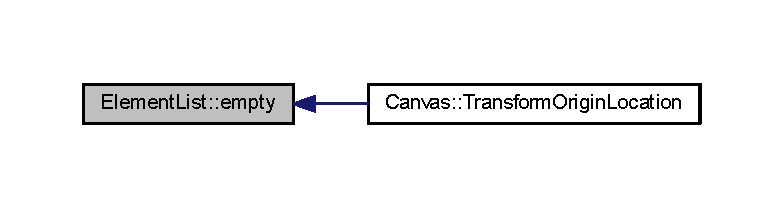
\includegraphics[width=350pt]{class_element_list_aff93ee82e54aa171e792b0a86cafd08a_icgraph}
\end{center}
\end{figure}
\mbox{\Hypertarget{class_element_list_a7e5dfdae6a16e385bbdd1564fd5cf200}\label{class_element_list_a7e5dfdae6a16e385bbdd1564fd5cf200}} 
\index{Element\+List@{Element\+List}!end@{end}}
\index{end@{end}!Element\+List@{Element\+List}}
\subsubsection{\texorpdfstring{end()}{end()}}
{\footnotesize\ttfamily \hyperlink{class_element_list_a10e1b0c17ebe441fcd035fcf0a00d25e}{iterator} Element\+List\+::end (\begin{DoxyParamCaption}{ }\end{DoxyParamCaption})\hspace{0.3cm}{\ttfamily [inline]}}



Definition at line 118 of file Graphical\+Element.\+h.

\mbox{\Hypertarget{class_element_list_a0c7327348fe7c7d8ad032ad4a71eed39}\label{class_element_list_a0c7327348fe7c7d8ad032ad4a71eed39}} 
\index{Element\+List@{Element\+List}!push\+\_\+back@{push\+\_\+back}}
\index{push\+\_\+back@{push\+\_\+back}!Element\+List@{Element\+List}}
\subsubsection{\texorpdfstring{push\+\_\+back()}{push\_back()}}
{\footnotesize\ttfamily void Element\+List\+::push\+\_\+back (\begin{DoxyParamCaption}\item[{\hyperlink{class_graphical_element}{Graphical\+Element} $\ast$}]{element }\end{DoxyParamCaption})\hspace{0.3cm}{\ttfamily [inline]}}



Definition at line 134 of file Graphical\+Element.\+h.

Here is the caller graph for this function\+:
\nopagebreak
\begin{figure}[H]
\begin{center}
\leavevmode
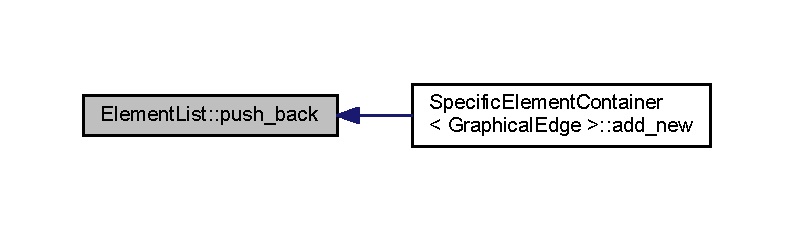
\includegraphics[width=350pt]{class_element_list_a0c7327348fe7c7d8ad032ad4a71eed39_icgraph}
\end{center}
\end{figure}
\mbox{\Hypertarget{class_element_list_a827726e626667715db21ad21f1b7d6fa}\label{class_element_list_a827726e626667715db21ad21f1b7d6fa}} 
\index{Element\+List@{Element\+List}!rbegin@{rbegin}}
\index{rbegin@{rbegin}!Element\+List@{Element\+List}}
\subsubsection{\texorpdfstring{rbegin()}{rbegin()}}
{\footnotesize\ttfamily \hyperlink{class_element_list_a5a94d1e25a0deeb3f222dc12fa115174}{reverse\+\_\+iterator} Element\+List\+::rbegin (\begin{DoxyParamCaption}{ }\end{DoxyParamCaption})\hspace{0.3cm}{\ttfamily [inline]}}



Definition at line 126 of file Graphical\+Element.\+h.

\mbox{\Hypertarget{class_element_list_a06b71e09b7ca85b416effbdac076ec49}\label{class_element_list_a06b71e09b7ca85b416effbdac076ec49}} 
\index{Element\+List@{Element\+List}!remove@{remove}}
\index{remove@{remove}!Element\+List@{Element\+List}}
\subsubsection{\texorpdfstring{remove()}{remove()}}
{\footnotesize\ttfamily void Element\+List\+::remove (\begin{DoxyParamCaption}\item[{\hyperlink{class_graphical_element}{Graphical\+Element} $\ast$}]{element }\end{DoxyParamCaption})\hspace{0.3cm}{\ttfamily [inline]}}



Definition at line 137 of file Graphical\+Element.\+h.

Here is the caller graph for this function\+:
\nopagebreak
\begin{figure}[H]
\begin{center}
\leavevmode
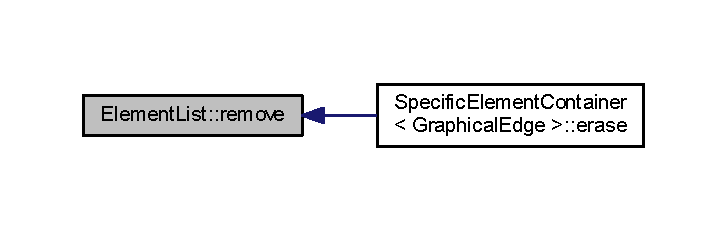
\includegraphics[width=349pt]{class_element_list_a06b71e09b7ca85b416effbdac076ec49_icgraph}
\end{center}
\end{figure}
\mbox{\Hypertarget{class_element_list_aa851e6d5b10920f2541d3dc0f5f2ee57}\label{class_element_list_aa851e6d5b10920f2541d3dc0f5f2ee57}} 
\index{Element\+List@{Element\+List}!remove\+\_\+if@{remove\+\_\+if}}
\index{remove\+\_\+if@{remove\+\_\+if}!Element\+List@{Element\+List}}
\subsubsection{\texorpdfstring{remove\+\_\+if()}{remove\_if()}}
{\footnotesize\ttfamily template$<$class \+\_\+\+Pr $>$ \\
void Element\+List\+::remove\+\_\+if (\begin{DoxyParamCaption}\item[{\+\_\+\+Pr}]{predicate }\end{DoxyParamCaption})\hspace{0.3cm}{\ttfamily [inline]}}



Definition at line 141 of file Graphical\+Element.\+h.

\mbox{\Hypertarget{class_element_list_a5c77af44a070ae80cddef7ce161e2f8b}\label{class_element_list_a5c77af44a070ae80cddef7ce161e2f8b}} 
\index{Element\+List@{Element\+List}!rend@{rend}}
\index{rend@{rend}!Element\+List@{Element\+List}}
\subsubsection{\texorpdfstring{rend()}{rend()}}
{\footnotesize\ttfamily \hyperlink{class_element_list_a5a94d1e25a0deeb3f222dc12fa115174}{reverse\+\_\+iterator} Element\+List\+::rend (\begin{DoxyParamCaption}{ }\end{DoxyParamCaption})\hspace{0.3cm}{\ttfamily [inline]}}



Definition at line 128 of file Graphical\+Element.\+h.



The documentation for this class was generated from the following files\+:\begin{DoxyCompactItemize}
\item 
Simulation Software/\+Source Files/\hyperlink{_graphical_element_8h}{Graphical\+Element.\+h}\item 
Simulation Software/\+Source Files/\hyperlink{_graphical_element_8cpp}{Graphical\+Element.\+cpp}\end{DoxyCompactItemize}

\hypertarget{class_s_s_s_q_1_1_end_processing_e_a}{}\section{S\+S\+SQ\+:\+:End\+Processing\+EA Class Reference}
\label{class_s_s_s_q_1_1_end_processing_e_a}\index{S\+S\+S\+Q\+::\+End\+Processing\+EA@{S\+S\+S\+Q\+::\+End\+Processing\+EA}}


Inheritance diagram for S\+S\+SQ\+:\+:End\+Processing\+EA\+:
\nopagebreak
\begin{figure}[H]
\begin{center}
\leavevmode
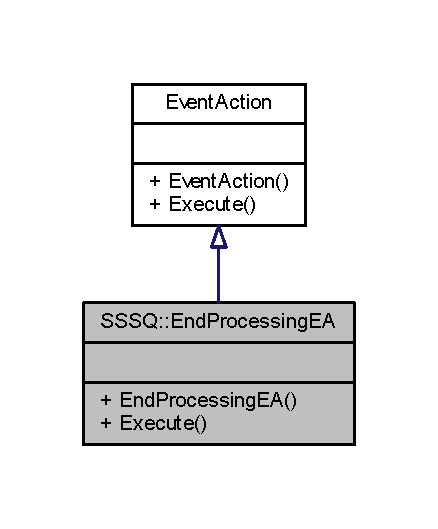
\includegraphics[width=210pt]{class_s_s_s_q_1_1_end_processing_e_a__inherit__graph}
\end{center}
\end{figure}


Collaboration diagram for S\+S\+SQ\+:\+:End\+Processing\+EA\+:
\nopagebreak
\begin{figure}[H]
\begin{center}
\leavevmode
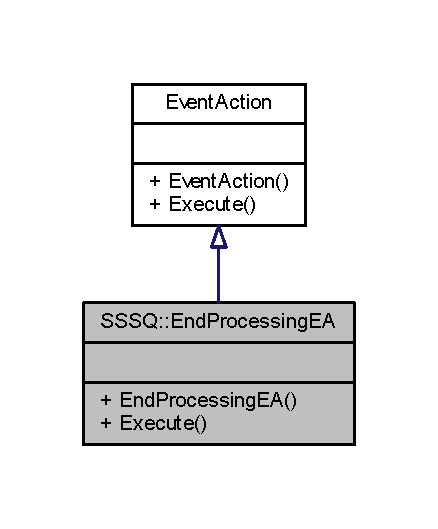
\includegraphics[width=210pt]{class_s_s_s_q_1_1_end_processing_e_a__coll__graph}
\end{center}
\end{figure}
\subsection*{Public Member Functions}
\begin{DoxyCompactItemize}
\item 
\hyperlink{class_s_s_s_q_1_1_end_processing_e_a_a0346a53be04c74fc6c6909693ffe94d3}{End\+Processing\+EA} (\hyperlink{class_s_s_s_q}{S\+S\+SQ} $\ast$s, \hyperlink{class_entity}{Entity} $\ast$e)
\item 
void \hyperlink{class_s_s_s_q_1_1_end_processing_e_a_a58123dc9ac0660bd1da11407e5467968}{Execute} ()
\end{DoxyCompactItemize}


\subsection{Detailed Description}


Definition at line 351 of file Specific\+Nodes.\+cpp.



\subsection{Constructor \& Destructor Documentation}
\mbox{\Hypertarget{class_s_s_s_q_1_1_end_processing_e_a_a0346a53be04c74fc6c6909693ffe94d3}\label{class_s_s_s_q_1_1_end_processing_e_a_a0346a53be04c74fc6c6909693ffe94d3}} 
\index{S\+S\+S\+Q\+::\+End\+Processing\+EA@{S\+S\+S\+Q\+::\+End\+Processing\+EA}!End\+Processing\+EA@{End\+Processing\+EA}}
\index{End\+Processing\+EA@{End\+Processing\+EA}!S\+S\+S\+Q\+::\+End\+Processing\+EA@{S\+S\+S\+Q\+::\+End\+Processing\+EA}}
\subsubsection{\texorpdfstring{End\+Processing\+E\+A()}{EndProcessingEA()}}
{\footnotesize\ttfamily S\+S\+S\+Q\+::\+End\+Processing\+E\+A\+::\+End\+Processing\+EA (\begin{DoxyParamCaption}\item[{\hyperlink{class_s_s_s_q}{S\+S\+SQ} $\ast$}]{s,  }\item[{\hyperlink{class_entity}{Entity} $\ast$}]{e }\end{DoxyParamCaption})\hspace{0.3cm}{\ttfamily [inline]}}



Definition at line 353 of file Specific\+Nodes.\+cpp.



\subsection{Member Function Documentation}
\mbox{\Hypertarget{class_s_s_s_q_1_1_end_processing_e_a_a58123dc9ac0660bd1da11407e5467968}\label{class_s_s_s_q_1_1_end_processing_e_a_a58123dc9ac0660bd1da11407e5467968}} 
\index{S\+S\+S\+Q\+::\+End\+Processing\+EA@{S\+S\+S\+Q\+::\+End\+Processing\+EA}!Execute@{Execute}}
\index{Execute@{Execute}!S\+S\+S\+Q\+::\+End\+Processing\+EA@{S\+S\+S\+Q\+::\+End\+Processing\+EA}}
\subsubsection{\texorpdfstring{Execute()}{Execute()}}
{\footnotesize\ttfamily void S\+S\+S\+Q\+::\+End\+Processing\+E\+A\+::\+Execute (\begin{DoxyParamCaption}{ }\end{DoxyParamCaption})\hspace{0.3cm}{\ttfamily [inline]}, {\ttfamily [virtual]}}



Implements \hyperlink{class_event_action_a62b9d07abb4ca8e7c078b076a1ab1a9f}{Event\+Action}.



Definition at line 358 of file Specific\+Nodes.\+cpp.



The documentation for this class was generated from the following file\+:\begin{DoxyCompactItemize}
\item 
Simulation Software/\+Source Files/\hyperlink{_specific_nodes_8cpp}{Specific\+Nodes.\+cpp}\end{DoxyCompactItemize}

\hypertarget{class_server_n_queue_1_1_end_processing_e_a}{}\section{Server\+N\+Queue\+:\+:End\+Processing\+EA Class Reference}
\label{class_server_n_queue_1_1_end_processing_e_a}\index{Server\+N\+Queue\+::\+End\+Processing\+EA@{Server\+N\+Queue\+::\+End\+Processing\+EA}}


Inheritance diagram for Server\+N\+Queue\+:\+:End\+Processing\+EA\+:
\nopagebreak
\begin{figure}[H]
\begin{center}
\leavevmode
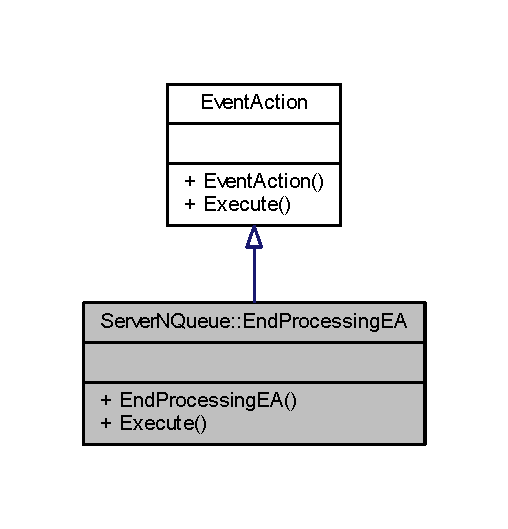
\includegraphics[width=244pt]{class_server_n_queue_1_1_end_processing_e_a__inherit__graph}
\end{center}
\end{figure}


Collaboration diagram for Server\+N\+Queue\+:\+:End\+Processing\+EA\+:
\nopagebreak
\begin{figure}[H]
\begin{center}
\leavevmode
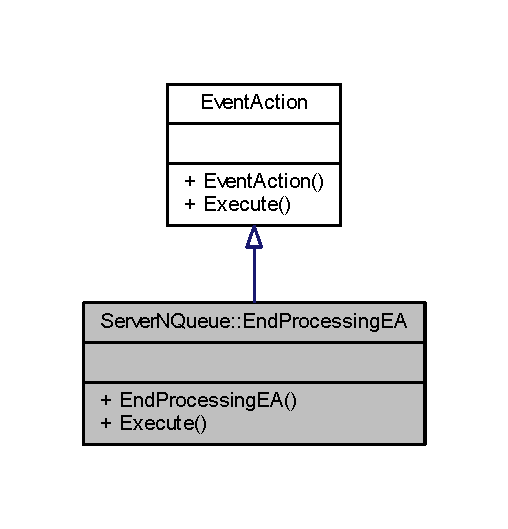
\includegraphics[width=244pt]{class_server_n_queue_1_1_end_processing_e_a__coll__graph}
\end{center}
\end{figure}
\subsection*{Public Member Functions}
\begin{DoxyCompactItemize}
\item 
\hyperlink{class_server_n_queue_1_1_end_processing_e_a_aa8fbe9861955c9893ab1341d65093c02}{End\+Processing\+EA} (\hyperlink{class_server_n_queue}{Server\+N\+Queue} $\ast$s, \hyperlink{class_entity}{Entity} $\ast$e)
\item 
void \hyperlink{class_server_n_queue_1_1_end_processing_e_a_a58033da71d12b3d61bf4c48f7c470e3d}{Execute} ()
\end{DoxyCompactItemize}


\subsection{Detailed Description}


Definition at line 559 of file Specific\+Nodes.\+cpp.



\subsection{Constructor \& Destructor Documentation}
\mbox{\Hypertarget{class_server_n_queue_1_1_end_processing_e_a_aa8fbe9861955c9893ab1341d65093c02}\label{class_server_n_queue_1_1_end_processing_e_a_aa8fbe9861955c9893ab1341d65093c02}} 
\index{Server\+N\+Queue\+::\+End\+Processing\+EA@{Server\+N\+Queue\+::\+End\+Processing\+EA}!End\+Processing\+EA@{End\+Processing\+EA}}
\index{End\+Processing\+EA@{End\+Processing\+EA}!Server\+N\+Queue\+::\+End\+Processing\+EA@{Server\+N\+Queue\+::\+End\+Processing\+EA}}
\subsubsection{\texorpdfstring{End\+Processing\+E\+A()}{EndProcessingEA()}}
{\footnotesize\ttfamily Server\+N\+Queue\+::\+End\+Processing\+E\+A\+::\+End\+Processing\+EA (\begin{DoxyParamCaption}\item[{\hyperlink{class_server_n_queue}{Server\+N\+Queue} $\ast$}]{s,  }\item[{\hyperlink{class_entity}{Entity} $\ast$}]{e }\end{DoxyParamCaption})\hspace{0.3cm}{\ttfamily [inline]}}



Definition at line 561 of file Specific\+Nodes.\+cpp.



\subsection{Member Function Documentation}
\mbox{\Hypertarget{class_server_n_queue_1_1_end_processing_e_a_a58033da71d12b3d61bf4c48f7c470e3d}\label{class_server_n_queue_1_1_end_processing_e_a_a58033da71d12b3d61bf4c48f7c470e3d}} 
\index{Server\+N\+Queue\+::\+End\+Processing\+EA@{Server\+N\+Queue\+::\+End\+Processing\+EA}!Execute@{Execute}}
\index{Execute@{Execute}!Server\+N\+Queue\+::\+End\+Processing\+EA@{Server\+N\+Queue\+::\+End\+Processing\+EA}}
\subsubsection{\texorpdfstring{Execute()}{Execute()}}
{\footnotesize\ttfamily void Server\+N\+Queue\+::\+End\+Processing\+E\+A\+::\+Execute (\begin{DoxyParamCaption}{ }\end{DoxyParamCaption})\hspace{0.3cm}{\ttfamily [inline]}, {\ttfamily [virtual]}}



Implements \hyperlink{class_event_action_a62b9d07abb4ca8e7c078b076a1ab1a9f}{Event\+Action}.



Definition at line 566 of file Specific\+Nodes.\+cpp.



The documentation for this class was generated from the following file\+:\begin{DoxyCompactItemize}
\item 
Simulation Software/\+Source Files/\hyperlink{_specific_nodes_8cpp}{Specific\+Nodes.\+cpp}\end{DoxyCompactItemize}

\hypertarget{class_entity}{}\section{Entity Class Reference}
\label{class_entity}\index{Entity@{Entity}}


{\ttfamily \#include $<$Entity.\+h$>$}



Inheritance diagram for Entity\+:\nopagebreak
\begin{figure}[H]
\begin{center}
\leavevmode
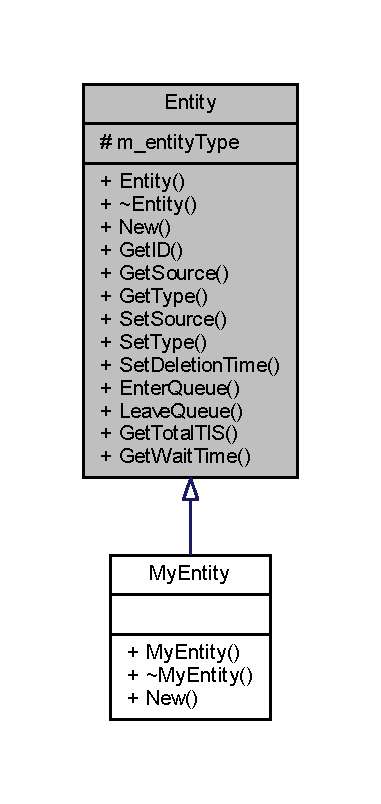
\includegraphics[width=183pt]{class_entity__inherit__graph}
\end{center}
\end{figure}


Collaboration diagram for Entity\+:\nopagebreak
\begin{figure}[H]
\begin{center}
\leavevmode
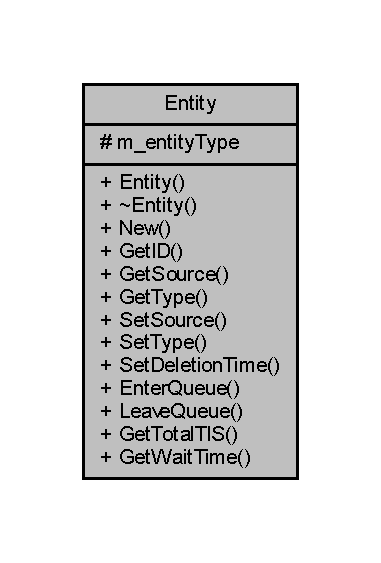
\includegraphics[width=183pt]{class_entity__coll__graph}
\end{center}
\end{figure}
\subsection*{Public Member Functions}
\begin{DoxyCompactItemize}
\item 
\hyperlink{class_entity_afb6488f2bb29b3e730459246e005dacd}{Entity} (\hyperlink{_simulation_executive_8h_ac2d3e0ba793497bcca555c7c2cf64ff3}{Time} creation\+Time)
\item 
\hyperlink{class_entity_adf6d3f7cb1b2ba029b6b048a395cc8ae}{$\sim$\+Entity} ()
\item 
virtual \hyperlink{class_entity}{Entity} $\ast$ \hyperlink{class_entity_ab8dc894a31d5c72219fa070345d7c383}{New} ()=0
\item 
int \hyperlink{class_entity_a8ed56bc59a6c2b0bd01eda3d274a1fac}{Get\+ID} ()
\item 
int \hyperlink{class_entity_a22d4fe26b229f7720f5204eeadffb1b2}{Get\+Source} ()
\item 
\hyperlink{_entity_8h_ad79a57ed3105eb60d991a1aeb4a9dc44}{Entity\+Type} \hyperlink{class_entity_a6618c119290b237bd6f9e903d029405d}{Get\+Type} ()
\item 
void \hyperlink{class_entity_ad08cf1231dbd8127e086bb803bdb3d5a}{Set\+Source} (int id)
\item 
void \hyperlink{class_entity_a91d4a101d4de57229710334b738bda29}{Set\+Type} (\hyperlink{_entity_8h_ad79a57ed3105eb60d991a1aeb4a9dc44}{Entity\+Type} my\+Type)
\item 
void \hyperlink{class_entity_a5c0dc393f667e2af24cd11d7b4bbd82c}{Set\+Deletion\+Time} (\hyperlink{_simulation_executive_8h_ac2d3e0ba793497bcca555c7c2cf64ff3}{Time} time\+Now)
\item 
void \hyperlink{class_entity_a957592ba81c76d59f622a887fee36e8d}{Enter\+Queue} (\hyperlink{_simulation_executive_8h_ac2d3e0ba793497bcca555c7c2cf64ff3}{Time} time\+Now)
\item 
\hyperlink{_simulation_executive_8h_ac2d3e0ba793497bcca555c7c2cf64ff3}{Time} \hyperlink{class_entity_ae05b43362e61b48a4a2ec5f629730029}{Leave\+Queue} (\hyperlink{_simulation_executive_8h_ac2d3e0ba793497bcca555c7c2cf64ff3}{Time} time\+Now)
\item 
\hyperlink{_simulation_executive_8h_ac2d3e0ba793497bcca555c7c2cf64ff3}{Time} \hyperlink{class_entity_abaed105c13bcd367823d4c1167e3042a}{Get\+Total\+T\+IS} ()
\item 
\hyperlink{_simulation_executive_8h_ac2d3e0ba793497bcca555c7c2cf64ff3}{Time} \hyperlink{class_entity_ae3fc482f0412da20727709c6659c8768}{Get\+Wait\+Time} ()
\end{DoxyCompactItemize}
\subsection*{Protected Attributes}
\begin{DoxyCompactItemize}
\item 
\hyperlink{_entity_8h_ad79a57ed3105eb60d991a1aeb4a9dc44}{Entity\+Type} \hyperlink{class_entity_a3431bdb8f5536c20eba5391e97e5ca8e}{m\+\_\+entity\+Type}
\end{DoxyCompactItemize}


\subsection{Detailed Description}


Definition at line 10 of file Entity.\+h.



\subsection{Constructor \& Destructor Documentation}
\mbox{\Hypertarget{class_entity_afb6488f2bb29b3e730459246e005dacd}\label{class_entity_afb6488f2bb29b3e730459246e005dacd}} 
\index{Entity@{Entity}!Entity@{Entity}}
\index{Entity@{Entity}!Entity@{Entity}}
\subsubsection{\texorpdfstring{Entity()}{Entity()}}
{\footnotesize\ttfamily Entity\+::\+Entity (\begin{DoxyParamCaption}\item[{\hyperlink{_simulation_executive_8h_ac2d3e0ba793497bcca555c7c2cf64ff3}{Time}}]{creation\+Time }\end{DoxyParamCaption})}



Definition at line 6 of file Entity.\+cpp.

\mbox{\Hypertarget{class_entity_adf6d3f7cb1b2ba029b6b048a395cc8ae}\label{class_entity_adf6d3f7cb1b2ba029b6b048a395cc8ae}} 
\index{Entity@{Entity}!````~Entity@{$\sim$\+Entity}}
\index{````~Entity@{$\sim$\+Entity}!Entity@{Entity}}
\subsubsection{\texorpdfstring{$\sim$\+Entity()}{~Entity()}}
{\footnotesize\ttfamily Entity\+::$\sim$\+Entity (\begin{DoxyParamCaption}{ }\end{DoxyParamCaption})\hspace{0.3cm}{\ttfamily [inline]}}



Definition at line 14 of file Entity.\+h.

Here is the call graph for this function\+:\nopagebreak
\begin{figure}[H]
\begin{center}
\leavevmode
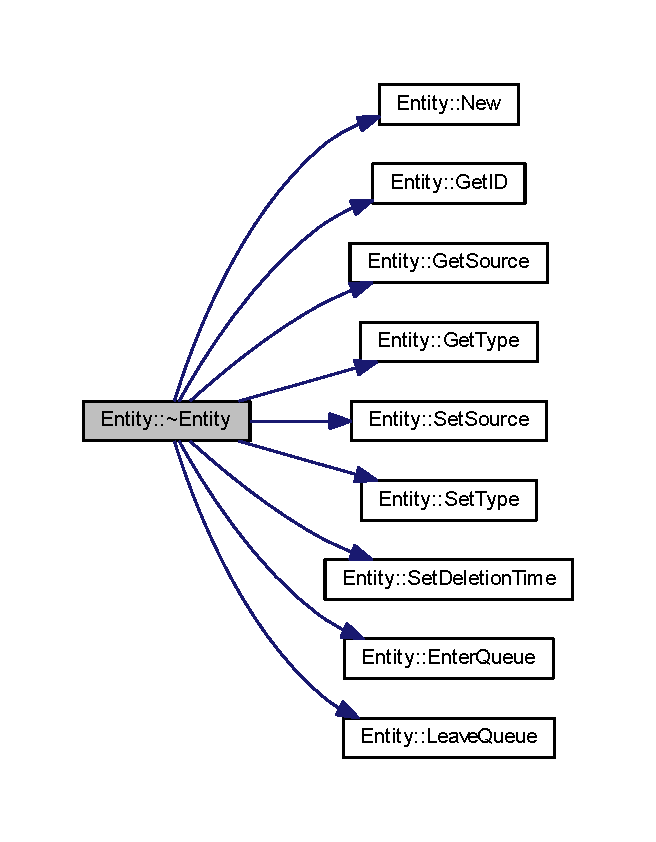
\includegraphics[width=315pt]{class_entity_adf6d3f7cb1b2ba029b6b048a395cc8ae_cgraph}
\end{center}
\end{figure}


\subsection{Member Function Documentation}
\mbox{\Hypertarget{class_entity_a957592ba81c76d59f622a887fee36e8d}\label{class_entity_a957592ba81c76d59f622a887fee36e8d}} 
\index{Entity@{Entity}!Enter\+Queue@{Enter\+Queue}}
\index{Enter\+Queue@{Enter\+Queue}!Entity@{Entity}}
\subsubsection{\texorpdfstring{Enter\+Queue()}{EnterQueue()}}
{\footnotesize\ttfamily void Entity\+::\+Enter\+Queue (\begin{DoxyParamCaption}\item[{\hyperlink{_simulation_executive_8h_ac2d3e0ba793497bcca555c7c2cf64ff3}{Time}}]{time\+Now }\end{DoxyParamCaption})}



Definition at line 39 of file Entity.\+cpp.

Here is the caller graph for this function\+:\nopagebreak
\begin{figure}[H]
\begin{center}
\leavevmode
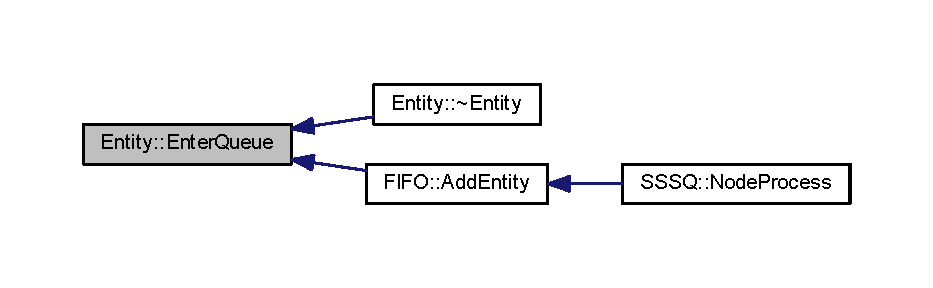
\includegraphics[width=350pt]{class_entity_a957592ba81c76d59f622a887fee36e8d_icgraph}
\end{center}
\end{figure}
\mbox{\Hypertarget{class_entity_a8ed56bc59a6c2b0bd01eda3d274a1fac}\label{class_entity_a8ed56bc59a6c2b0bd01eda3d274a1fac}} 
\index{Entity@{Entity}!Get\+ID@{Get\+ID}}
\index{Get\+ID@{Get\+ID}!Entity@{Entity}}
\subsubsection{\texorpdfstring{Get\+I\+D()}{GetID()}}
{\footnotesize\ttfamily int Entity\+::\+Get\+ID (\begin{DoxyParamCaption}{ }\end{DoxyParamCaption})}



Definition at line 19 of file Entity.\+cpp.

Here is the caller graph for this function\+:
\nopagebreak
\begin{figure}[H]
\begin{center}
\leavevmode
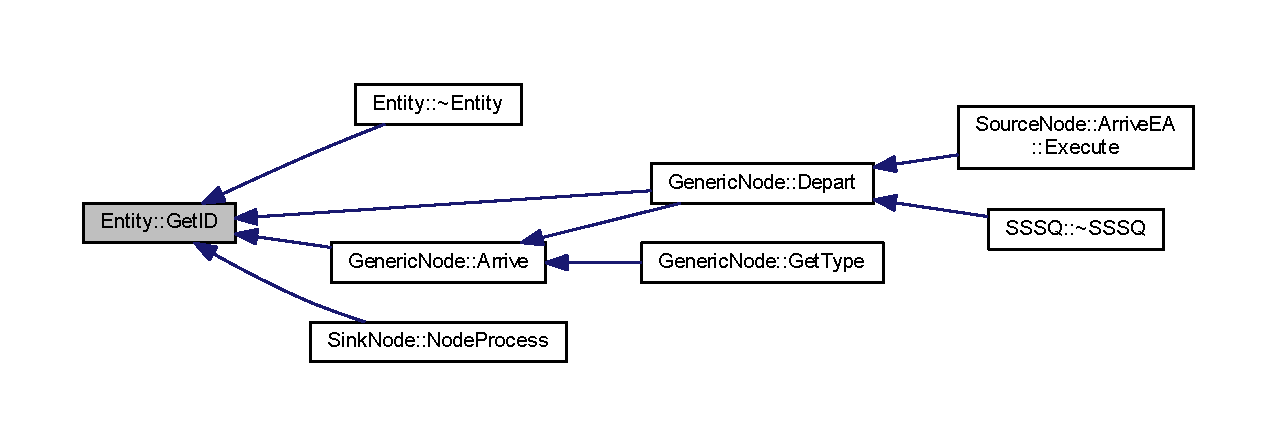
\includegraphics[width=350pt]{class_entity_a8ed56bc59a6c2b0bd01eda3d274a1fac_icgraph}
\end{center}
\end{figure}
\mbox{\Hypertarget{class_entity_a22d4fe26b229f7720f5204eeadffb1b2}\label{class_entity_a22d4fe26b229f7720f5204eeadffb1b2}} 
\index{Entity@{Entity}!Get\+Source@{Get\+Source}}
\index{Get\+Source@{Get\+Source}!Entity@{Entity}}
\subsubsection{\texorpdfstring{Get\+Source()}{GetSource()}}
{\footnotesize\ttfamily int Entity\+::\+Get\+Source (\begin{DoxyParamCaption}{ }\end{DoxyParamCaption})}



Definition at line 57 of file Entity.\+cpp.

Here is the caller graph for this function\+:\nopagebreak
\begin{figure}[H]
\begin{center}
\leavevmode
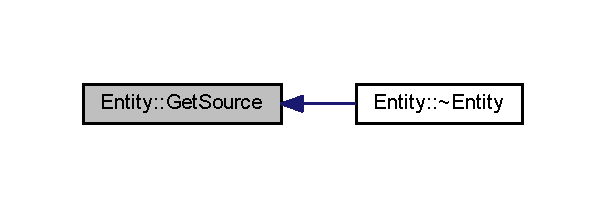
\includegraphics[width=291pt]{class_entity_a22d4fe26b229f7720f5204eeadffb1b2_icgraph}
\end{center}
\end{figure}
\mbox{\Hypertarget{class_entity_abaed105c13bcd367823d4c1167e3042a}\label{class_entity_abaed105c13bcd367823d4c1167e3042a}} 
\index{Entity@{Entity}!Get\+Total\+T\+IS@{Get\+Total\+T\+IS}}
\index{Get\+Total\+T\+IS@{Get\+Total\+T\+IS}!Entity@{Entity}}
\subsubsection{\texorpdfstring{Get\+Total\+T\+I\+S()}{GetTotalTIS()}}
{\footnotesize\ttfamily \hyperlink{_simulation_executive_8h_ac2d3e0ba793497bcca555c7c2cf64ff3}{Time} Entity\+::\+Get\+Total\+T\+IS (\begin{DoxyParamCaption}{ }\end{DoxyParamCaption})\hspace{0.3cm}{\ttfamily [inline]}}



Definition at line 32 of file Entity.\+h.

\mbox{\Hypertarget{class_entity_a6618c119290b237bd6f9e903d029405d}\label{class_entity_a6618c119290b237bd6f9e903d029405d}} 
\index{Entity@{Entity}!Get\+Type@{Get\+Type}}
\index{Get\+Type@{Get\+Type}!Entity@{Entity}}
\subsubsection{\texorpdfstring{Get\+Type()}{GetType()}}
{\footnotesize\ttfamily \hyperlink{_entity_8h_ad79a57ed3105eb60d991a1aeb4a9dc44}{Entity\+Type} Entity\+::\+Get\+Type (\begin{DoxyParamCaption}{ }\end{DoxyParamCaption})}



Definition at line 34 of file Entity.\+cpp.

Here is the caller graph for this function\+:\nopagebreak
\begin{figure}[H]
\begin{center}
\leavevmode
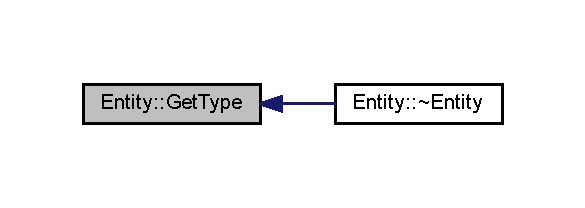
\includegraphics[width=281pt]{class_entity_a6618c119290b237bd6f9e903d029405d_icgraph}
\end{center}
\end{figure}
\mbox{\Hypertarget{class_entity_ae3fc482f0412da20727709c6659c8768}\label{class_entity_ae3fc482f0412da20727709c6659c8768}} 
\index{Entity@{Entity}!Get\+Wait\+Time@{Get\+Wait\+Time}}
\index{Get\+Wait\+Time@{Get\+Wait\+Time}!Entity@{Entity}}
\subsubsection{\texorpdfstring{Get\+Wait\+Time()}{GetWaitTime()}}
{\footnotesize\ttfamily \hyperlink{_simulation_executive_8h_ac2d3e0ba793497bcca555c7c2cf64ff3}{Time} Entity\+::\+Get\+Wait\+Time (\begin{DoxyParamCaption}{ }\end{DoxyParamCaption})\hspace{0.3cm}{\ttfamily [inline]}}



Definition at line 33 of file Entity.\+h.

Here is the caller graph for this function\+:\nopagebreak
\begin{figure}[H]
\begin{center}
\leavevmode
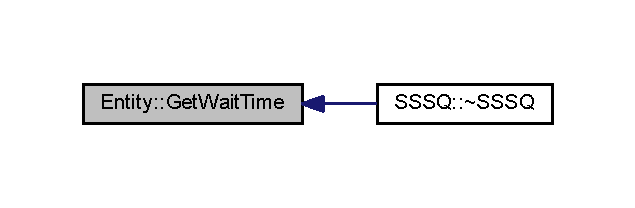
\includegraphics[width=305pt]{class_entity_ae3fc482f0412da20727709c6659c8768_icgraph}
\end{center}
\end{figure}
\mbox{\Hypertarget{class_entity_ae05b43362e61b48a4a2ec5f629730029}\label{class_entity_ae05b43362e61b48a4a2ec5f629730029}} 
\index{Entity@{Entity}!Leave\+Queue@{Leave\+Queue}}
\index{Leave\+Queue@{Leave\+Queue}!Entity@{Entity}}
\subsubsection{\texorpdfstring{Leave\+Queue()}{LeaveQueue()}}
{\footnotesize\ttfamily \hyperlink{_simulation_executive_8h_ac2d3e0ba793497bcca555c7c2cf64ff3}{Time} Entity\+::\+Leave\+Queue (\begin{DoxyParamCaption}\item[{\hyperlink{_simulation_executive_8h_ac2d3e0ba793497bcca555c7c2cf64ff3}{Time}}]{time\+Now }\end{DoxyParamCaption})}



Definition at line 44 of file Entity.\+cpp.

Here is the caller graph for this function\+:\nopagebreak
\begin{figure}[H]
\begin{center}
\leavevmode
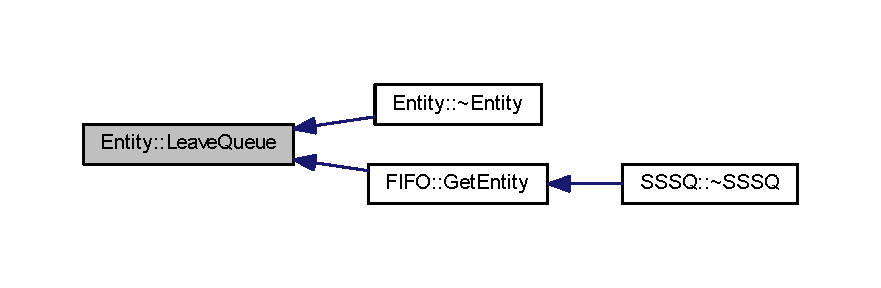
\includegraphics[width=350pt]{class_entity_ae05b43362e61b48a4a2ec5f629730029_icgraph}
\end{center}
\end{figure}
\mbox{\Hypertarget{class_entity_ab8dc894a31d5c72219fa070345d7c383}\label{class_entity_ab8dc894a31d5c72219fa070345d7c383}} 
\index{Entity@{Entity}!New@{New}}
\index{New@{New}!Entity@{Entity}}
\subsubsection{\texorpdfstring{New()}{New()}}
{\footnotesize\ttfamily virtual \hyperlink{class_entity}{Entity}$\ast$ Entity\+::\+New (\begin{DoxyParamCaption}{ }\end{DoxyParamCaption})\hspace{0.3cm}{\ttfamily [pure virtual]}}



Implemented in \hyperlink{class_my_entity_acc29e753a0df1928eb4c9e627d65a3b3}{My\+Entity}.

Here is the caller graph for this function\+:\nopagebreak
\begin{figure}[H]
\begin{center}
\leavevmode
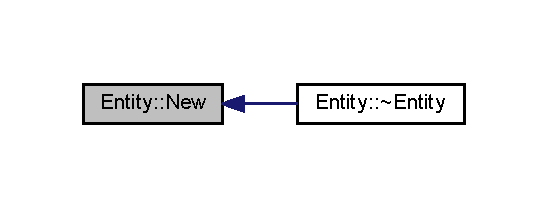
\includegraphics[width=263pt]{class_entity_ab8dc894a31d5c72219fa070345d7c383_icgraph}
\end{center}
\end{figure}
\mbox{\Hypertarget{class_entity_a5c0dc393f667e2af24cd11d7b4bbd82c}\label{class_entity_a5c0dc393f667e2af24cd11d7b4bbd82c}} 
\index{Entity@{Entity}!Set\+Deletion\+Time@{Set\+Deletion\+Time}}
\index{Set\+Deletion\+Time@{Set\+Deletion\+Time}!Entity@{Entity}}
\subsubsection{\texorpdfstring{Set\+Deletion\+Time()}{SetDeletionTime()}}
{\footnotesize\ttfamily void Entity\+::\+Set\+Deletion\+Time (\begin{DoxyParamCaption}\item[{\hyperlink{_simulation_executive_8h_ac2d3e0ba793497bcca555c7c2cf64ff3}{Time}}]{time\+Now }\end{DoxyParamCaption})}



Definition at line 29 of file Entity.\+cpp.

Here is the caller graph for this function\+:\nopagebreak
\begin{figure}[H]
\begin{center}
\leavevmode
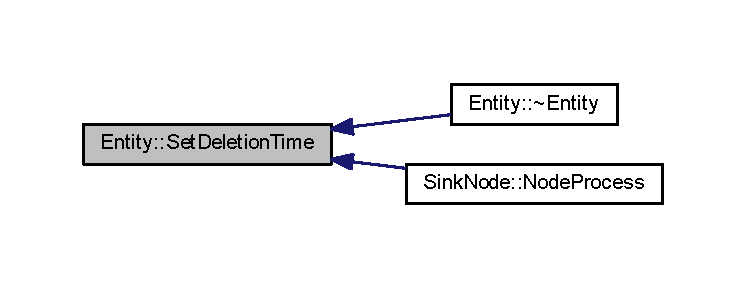
\includegraphics[width=350pt]{class_entity_a5c0dc393f667e2af24cd11d7b4bbd82c_icgraph}
\end{center}
\end{figure}
\mbox{\Hypertarget{class_entity_ad08cf1231dbd8127e086bb803bdb3d5a}\label{class_entity_ad08cf1231dbd8127e086bb803bdb3d5a}} 
\index{Entity@{Entity}!Set\+Source@{Set\+Source}}
\index{Set\+Source@{Set\+Source}!Entity@{Entity}}
\subsubsection{\texorpdfstring{Set\+Source()}{SetSource()}}
{\footnotesize\ttfamily void Entity\+::\+Set\+Source (\begin{DoxyParamCaption}\item[{int}]{id }\end{DoxyParamCaption})}



Definition at line 52 of file Entity.\+cpp.

Here is the caller graph for this function\+:\nopagebreak
\begin{figure}[H]
\begin{center}
\leavevmode
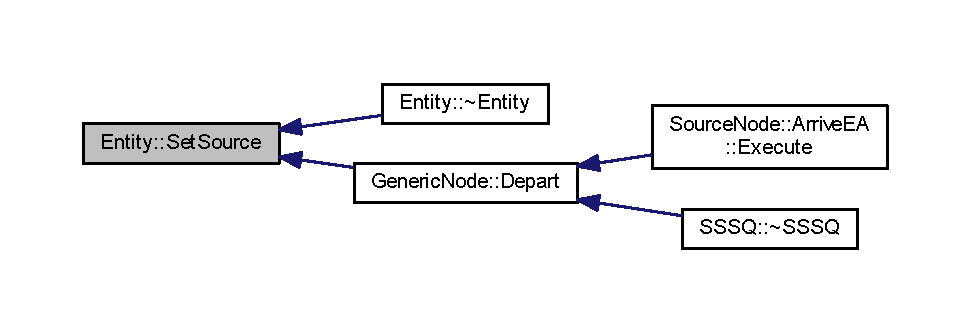
\includegraphics[width=350pt]{class_entity_ad08cf1231dbd8127e086bb803bdb3d5a_icgraph}
\end{center}
\end{figure}
\mbox{\Hypertarget{class_entity_a91d4a101d4de57229710334b738bda29}\label{class_entity_a91d4a101d4de57229710334b738bda29}} 
\index{Entity@{Entity}!Set\+Type@{Set\+Type}}
\index{Set\+Type@{Set\+Type}!Entity@{Entity}}
\subsubsection{\texorpdfstring{Set\+Type()}{SetType()}}
{\footnotesize\ttfamily void Entity\+::\+Set\+Type (\begin{DoxyParamCaption}\item[{\hyperlink{_entity_8h_ad79a57ed3105eb60d991a1aeb4a9dc44}{Entity\+Type}}]{my\+Type }\end{DoxyParamCaption})}



Definition at line 24 of file Entity.\+cpp.

Here is the caller graph for this function\+:\nopagebreak
\begin{figure}[H]
\begin{center}
\leavevmode
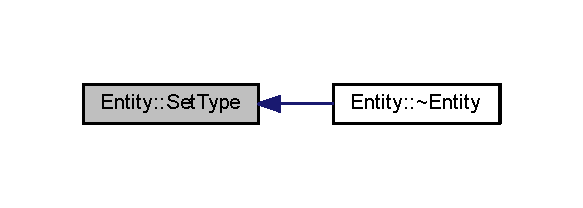
\includegraphics[width=280pt]{class_entity_a91d4a101d4de57229710334b738bda29_icgraph}
\end{center}
\end{figure}


\subsection{Member Data Documentation}
\mbox{\Hypertarget{class_entity_a3431bdb8f5536c20eba5391e97e5ca8e}\label{class_entity_a3431bdb8f5536c20eba5391e97e5ca8e}} 
\index{Entity@{Entity}!m\+\_\+entity\+Type@{m\+\_\+entity\+Type}}
\index{m\+\_\+entity\+Type@{m\+\_\+entity\+Type}!Entity@{Entity}}
\subsubsection{\texorpdfstring{m\+\_\+entity\+Type}{m\_entityType}}
{\footnotesize\ttfamily \hyperlink{_entity_8h_ad79a57ed3105eb60d991a1aeb4a9dc44}{Entity\+Type} Entity\+::m\+\_\+entity\+Type\hspace{0.3cm}{\ttfamily [protected]}}



Definition at line 36 of file Entity.\+h.



The documentation for this class was generated from the following files\+:\begin{DoxyCompactItemize}
\item 
Simulation Software/\+Source Files/\hyperlink{_entity_8h}{Entity.\+h}\item 
Simulation Software/\+Source Files/\hyperlink{_entity_8cpp}{Entity.\+cpp}\end{DoxyCompactItemize}

\hypertarget{class_erlang}{}\section{Erlang Class Reference}
\label{class_erlang}\index{Erlang@{Erlang}}


{\ttfamily \#include $<$Distribution.\+h$>$}



Inheritance diagram for Erlang\+:
\nopagebreak
\begin{figure}[H]
\begin{center}
\leavevmode
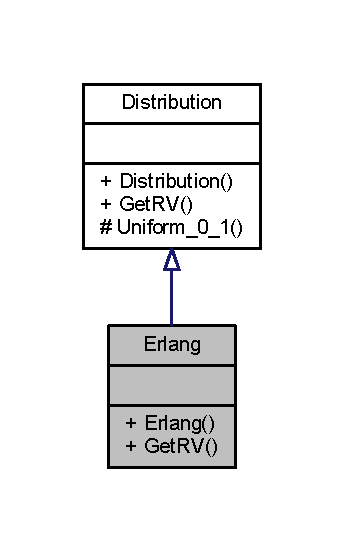
\includegraphics[width=165pt]{class_erlang__inherit__graph}
\end{center}
\end{figure}


Collaboration diagram for Erlang\+:
\nopagebreak
\begin{figure}[H]
\begin{center}
\leavevmode
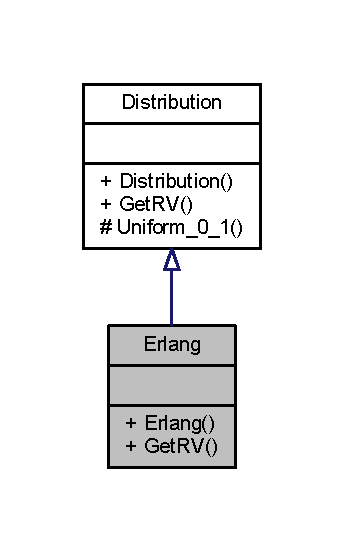
\includegraphics[width=165pt]{class_erlang__coll__graph}
\end{center}
\end{figure}
\subsection*{Public Member Functions}
\begin{DoxyCompactItemize}
\item 
\hyperlink{class_erlang_a5799b0314c8400cdb318df37625de98e}{Erlang} (int scale, double shape)
\item 
double \hyperlink{class_erlang_a5ae5b56e37bd2c5ee4318fcc12259442}{Get\+RV} ()
\end{DoxyCompactItemize}
\subsection*{Additional Inherited Members}


\subsection{Detailed Description}


Definition at line 79 of file Distribution.\+h.



\subsection{Constructor \& Destructor Documentation}
\mbox{\Hypertarget{class_erlang_a5799b0314c8400cdb318df37625de98e}\label{class_erlang_a5799b0314c8400cdb318df37625de98e}} 
\index{Erlang@{Erlang}!Erlang@{Erlang}}
\index{Erlang@{Erlang}!Erlang@{Erlang}}
\subsubsection{\texorpdfstring{Erlang()}{Erlang()}}
{\footnotesize\ttfamily Erlang\+::\+Erlang (\begin{DoxyParamCaption}\item[{int}]{scale,  }\item[{double}]{shape }\end{DoxyParamCaption})}



Definition at line 114 of file Distribution.\+cpp.



\subsection{Member Function Documentation}
\mbox{\Hypertarget{class_erlang_a5ae5b56e37bd2c5ee4318fcc12259442}\label{class_erlang_a5ae5b56e37bd2c5ee4318fcc12259442}} 
\index{Erlang@{Erlang}!Get\+RV@{Get\+RV}}
\index{Get\+RV@{Get\+RV}!Erlang@{Erlang}}
\subsubsection{\texorpdfstring{Get\+R\+V()}{GetRV()}}
{\footnotesize\ttfamily double Erlang\+::\+Get\+RV (\begin{DoxyParamCaption}{ }\end{DoxyParamCaption})\hspace{0.3cm}{\ttfamily [virtual]}}



Implements \hyperlink{class_distribution_a63b433850d7b47d84eb69448f7916719}{Distribution}.



Definition at line 120 of file Distribution.\+cpp.

Here is the call graph for this function\+:
\nopagebreak
\begin{figure}[H]
\begin{center}
\leavevmode
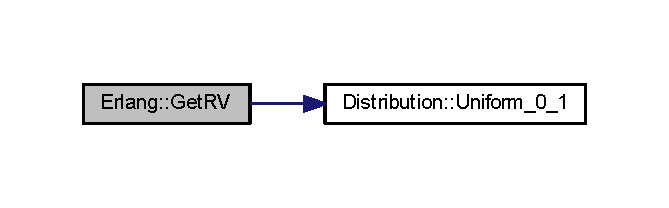
\includegraphics[width=321pt]{class_erlang_a5ae5b56e37bd2c5ee4318fcc12259442_cgraph}
\end{center}
\end{figure}


The documentation for this class was generated from the following files\+:\begin{DoxyCompactItemize}
\item 
Simulation Software/\+Source Files/\hyperlink{_distribution_8h}{Distribution.\+h}\item 
Simulation Software/\+Source Files/\hyperlink{_distribution_8cpp}{Distribution.\+cpp}\end{DoxyCompactItemize}

\hypertarget{struct_event}{}\section{Event Struct Reference}
\label{struct_event}\index{Event@{Event}}


Collaboration diagram for Event\+:
\nopagebreak
\begin{figure}[H]
\begin{center}
\leavevmode
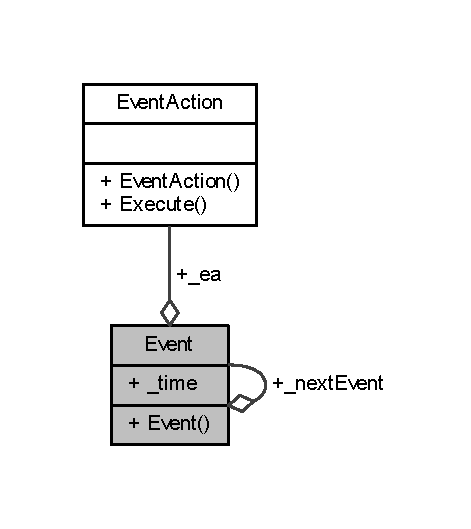
\includegraphics[width=226pt]{struct_event__coll__graph}
\end{center}
\end{figure}
\subsection*{Public Member Functions}
\begin{DoxyCompactItemize}
\item 
\hyperlink{struct_event_a5236b45d6ac7c6ce784c3e39fed03d7d}{Event} (\hyperlink{_simulation_executive_8h_ac2d3e0ba793497bcca555c7c2cf64ff3}{Time} time, \hyperlink{class_event_action}{Event\+Action} $\ast$ea)
\end{DoxyCompactItemize}
\subsection*{Public Attributes}
\begin{DoxyCompactItemize}
\item 
\hyperlink{_simulation_executive_8h_ac2d3e0ba793497bcca555c7c2cf64ff3}{Time} \hyperlink{struct_event_a7077d3af8bbf3d40e3c4570cc4675512}{\+\_\+time}
\item 
\hyperlink{class_event_action}{Event\+Action} $\ast$ \hyperlink{struct_event_aacbbfbf051167338e9febaaa5aad5b73}{\+\_\+ea}
\item 
\hyperlink{struct_event}{Event} $\ast$ \hyperlink{struct_event_a6bc8ec440b4f0b617d58af059e44e43e}{\+\_\+next\+Event}
\end{DoxyCompactItemize}


\subsection{Detailed Description}


Definition at line 8 of file Simulation\+Executive.\+cpp.



\subsection{Constructor \& Destructor Documentation}
\mbox{\Hypertarget{struct_event_a5236b45d6ac7c6ce784c3e39fed03d7d}\label{struct_event_a5236b45d6ac7c6ce784c3e39fed03d7d}} 
\index{Event@{Event}!Event@{Event}}
\index{Event@{Event}!Event@{Event}}
\subsubsection{\texorpdfstring{Event()}{Event()}}
{\footnotesize\ttfamily Event\+::\+Event (\begin{DoxyParamCaption}\item[{\hyperlink{_simulation_executive_8h_ac2d3e0ba793497bcca555c7c2cf64ff3}{Time}}]{time,  }\item[{\hyperlink{class_event_action}{Event\+Action} $\ast$}]{ea }\end{DoxyParamCaption})\hspace{0.3cm}{\ttfamily [inline]}}



Definition at line 10 of file Simulation\+Executive.\+cpp.



\subsection{Member Data Documentation}
\mbox{\Hypertarget{struct_event_aacbbfbf051167338e9febaaa5aad5b73}\label{struct_event_aacbbfbf051167338e9febaaa5aad5b73}} 
\index{Event@{Event}!\+\_\+ea@{\+\_\+ea}}
\index{\+\_\+ea@{\+\_\+ea}!Event@{Event}}
\subsubsection{\texorpdfstring{\+\_\+ea}{\_ea}}
{\footnotesize\ttfamily \hyperlink{class_event_action}{Event\+Action}$\ast$ Event\+::\+\_\+ea}



Definition at line 17 of file Simulation\+Executive.\+cpp.

\mbox{\Hypertarget{struct_event_a6bc8ec440b4f0b617d58af059e44e43e}\label{struct_event_a6bc8ec440b4f0b617d58af059e44e43e}} 
\index{Event@{Event}!\+\_\+next\+Event@{\+\_\+next\+Event}}
\index{\+\_\+next\+Event@{\+\_\+next\+Event}!Event@{Event}}
\subsubsection{\texorpdfstring{\+\_\+next\+Event}{\_nextEvent}}
{\footnotesize\ttfamily \hyperlink{struct_event}{Event}$\ast$ Event\+::\+\_\+next\+Event}



Definition at line 18 of file Simulation\+Executive.\+cpp.

\mbox{\Hypertarget{struct_event_a7077d3af8bbf3d40e3c4570cc4675512}\label{struct_event_a7077d3af8bbf3d40e3c4570cc4675512}} 
\index{Event@{Event}!\+\_\+time@{\+\_\+time}}
\index{\+\_\+time@{\+\_\+time}!Event@{Event}}
\subsubsection{\texorpdfstring{\+\_\+time}{\_time}}
{\footnotesize\ttfamily \hyperlink{_simulation_executive_8h_ac2d3e0ba793497bcca555c7c2cf64ff3}{Time} Event\+::\+\_\+time}



Definition at line 16 of file Simulation\+Executive.\+cpp.



The documentation for this struct was generated from the following file\+:\begin{DoxyCompactItemize}
\item 
Simulation Software/\+Source Files/\hyperlink{_simulation_executive_8cpp}{Simulation\+Executive.\+cpp}\end{DoxyCompactItemize}

\hypertarget{class_event_action}{}\section{Event\+Action Class Reference}
\label{class_event_action}\index{Event\+Action@{Event\+Action}}


{\ttfamily \#include $<$Simulation\+Executive.\+h$>$}



Inheritance diagram for Event\+Action\+:\nopagebreak
\begin{figure}[H]
\begin{center}
\leavevmode
\includegraphics[width=350pt]{class_event_action__inherit__graph}
\end{center}
\end{figure}


Collaboration diagram for Event\+Action\+:\nopagebreak
\begin{figure}[H]
\begin{center}
\leavevmode
\includegraphics[width=163pt]{class_event_action__coll__graph}
\end{center}
\end{figure}
\subsection*{Public Member Functions}
\begin{DoxyCompactItemize}
\item 
\hyperlink{class_event_action_a9a8515b9069293b94b72a6863c48e6ba}{Event\+Action} ()
\item 
virtual void \hyperlink{class_event_action_a62b9d07abb4ca8e7c078b076a1ab1a9f}{Execute} ()=0
\end{DoxyCompactItemize}


\subsection{Detailed Description}


Definition at line 21 of file Simulation\+Executive.\+h.



\subsection{Constructor \& Destructor Documentation}
\mbox{\Hypertarget{class_event_action_a9a8515b9069293b94b72a6863c48e6ba}\label{class_event_action_a9a8515b9069293b94b72a6863c48e6ba}} 
\index{Event\+Action@{Event\+Action}!Event\+Action@{Event\+Action}}
\index{Event\+Action@{Event\+Action}!Event\+Action@{Event\+Action}}
\subsubsection{\texorpdfstring{Event\+Action()}{EventAction()}}
{\footnotesize\ttfamily Event\+Action\+::\+Event\+Action (\begin{DoxyParamCaption}{ }\end{DoxyParamCaption})\hspace{0.3cm}{\ttfamily [inline]}}



Definition at line 24 of file Simulation\+Executive.\+h.

Here is the call graph for this function\+:\nopagebreak
\begin{figure}[H]
\begin{center}
\leavevmode
\includegraphics[width=350pt]{class_event_action_a9a8515b9069293b94b72a6863c48e6ba_cgraph}
\end{center}
\end{figure}


\subsection{Member Function Documentation}
\mbox{\Hypertarget{class_event_action_a62b9d07abb4ca8e7c078b076a1ab1a9f}\label{class_event_action_a62b9d07abb4ca8e7c078b076a1ab1a9f}} 
\index{Event\+Action@{Event\+Action}!Execute@{Execute}}
\index{Execute@{Execute}!Event\+Action@{Event\+Action}}
\subsubsection{\texorpdfstring{Execute()}{Execute()}}
{\footnotesize\ttfamily virtual void Event\+Action\+::\+Execute (\begin{DoxyParamCaption}{ }\end{DoxyParamCaption})\hspace{0.3cm}{\ttfamily [pure virtual]}}



Implemented in \hyperlink{class_server_n_queue_1_1_end_processing_e_a_a58033da71d12b3d61bf4c48f7c470e3d}{Server\+N\+Queue\+::\+End\+Processing\+EA}, \hyperlink{class_server_n_queue_1_1_start_processing_e_a_a734000fd4380b39594df88706f674dd0}{Server\+N\+Queue\+::\+Start\+Processing\+EA}, \hyperlink{class_s_s_s_q_1_1_end_processing_e_a_a58123dc9ac0660bd1da11407e5467968}{S\+S\+S\+Q\+::\+End\+Processing\+EA}, \hyperlink{class_s_s_s_q_1_1_start_processing_e_a_a8734cd511dc7e4fd7f981ed2acb338cb}{S\+S\+S\+Q\+::\+Start\+Processing\+EA}, and \hyperlink{class_source_node_1_1_arrive_e_a_a622b2282aae023818b26d39519143c15}{Source\+Node\+::\+Arrive\+EA}.

Here is the caller graph for this function\+:
\nopagebreak
\begin{figure}[H]
\begin{center}
\leavevmode
\includegraphics[width=350pt]{class_event_action_a62b9d07abb4ca8e7c078b076a1ab1a9f_icgraph}
\end{center}
\end{figure}


The documentation for this class was generated from the following file\+:\begin{DoxyCompactItemize}
\item 
Simulation Software/\+Source Files/\hyperlink{_simulation_executive_8h}{Simulation\+Executive.\+h}\end{DoxyCompactItemize}

\hypertarget{class_exponential}{}\section{Exponential Class Reference}
\label{class_exponential}\index{Exponential@{Exponential}}


{\ttfamily \#include $<$Distribution.\+h$>$}



Inheritance diagram for Exponential\+:\nopagebreak
\begin{figure}[H]
\begin{center}
\leavevmode
\includegraphics[width=165pt]{class_exponential__inherit__graph}
\end{center}
\end{figure}


Collaboration diagram for Exponential\+:\nopagebreak
\begin{figure}[H]
\begin{center}
\leavevmode
\includegraphics[width=165pt]{class_exponential__coll__graph}
\end{center}
\end{figure}
\subsection*{Public Member Functions}
\begin{DoxyCompactItemize}
\item 
\hyperlink{class_exponential_aa135f2007ad33e977c019e9598f1d208}{Exponential} (double mean)
\item 
double \hyperlink{class_exponential_a2a45aeaf0a3725174d86712761a8dd82}{Get\+RV} ()
\end{DoxyCompactItemize}
\subsection*{Additional Inherited Members}


\subsection{Detailed Description}


Definition at line 13 of file Distribution.\+h.



\subsection{Constructor \& Destructor Documentation}
\mbox{\Hypertarget{class_exponential_aa135f2007ad33e977c019e9598f1d208}\label{class_exponential_aa135f2007ad33e977c019e9598f1d208}} 
\index{Exponential@{Exponential}!Exponential@{Exponential}}
\index{Exponential@{Exponential}!Exponential@{Exponential}}
\subsubsection{\texorpdfstring{Exponential()}{Exponential()}}
{\footnotesize\ttfamily Exponential\+::\+Exponential (\begin{DoxyParamCaption}\item[{double}]{mean }\end{DoxyParamCaption})}



Definition at line 12 of file Distribution.\+cpp.



\subsection{Member Function Documentation}
\mbox{\Hypertarget{class_exponential_a2a45aeaf0a3725174d86712761a8dd82}\label{class_exponential_a2a45aeaf0a3725174d86712761a8dd82}} 
\index{Exponential@{Exponential}!Get\+RV@{Get\+RV}}
\index{Get\+RV@{Get\+RV}!Exponential@{Exponential}}
\subsubsection{\texorpdfstring{Get\+R\+V()}{GetRV()}}
{\footnotesize\ttfamily double Exponential\+::\+Get\+RV (\begin{DoxyParamCaption}{ }\end{DoxyParamCaption})\hspace{0.3cm}{\ttfamily [virtual]}}



Implements \hyperlink{class_distribution_a63b433850d7b47d84eb69448f7916719}{Distribution}.



Definition at line 17 of file Distribution.\+cpp.

Here is the call graph for this function\+:\nopagebreak
\begin{figure}[H]
\begin{center}
\leavevmode
\includegraphics[width=344pt]{class_exponential_a2a45aeaf0a3725174d86712761a8dd82_cgraph}
\end{center}
\end{figure}


The documentation for this class was generated from the following files\+:\begin{DoxyCompactItemize}
\item 
Simulation Software/\+Source Files/\hyperlink{_distribution_8h}{Distribution.\+h}\item 
Simulation Software/\+Source Files/\hyperlink{_distribution_8cpp}{Distribution.\+cpp}\end{DoxyCompactItemize}

\hypertarget{class_f_i_f_o}{}\section{F\+I\+FO Class Reference}
\label{class_f_i_f_o}\index{F\+I\+FO@{F\+I\+FO}}


{\ttfamily \#include $<$F\+I\+F\+O.\+h$>$}



Collaboration diagram for F\+I\+FO\+:
\nopagebreak
\begin{figure}[H]
\begin{center}
\leavevmode
\includegraphics[width=218pt]{class_f_i_f_o__coll__graph}
\end{center}
\end{figure}
\subsection*{Public Member Functions}
\begin{DoxyCompactItemize}
\item 
\hyperlink{class_f_i_f_o_aea969385961885a8e70732482d64fead}{F\+I\+FO} ()
\item 
void \hyperlink{class_f_i_f_o_a7255ba93981ed0662bc4c26d9983dc9e}{Add\+Entity} (\hyperlink{class_entity}{Entity} $\ast$e)
\item 
\hyperlink{class_entity}{Entity} $\ast$ \hyperlink{class_f_i_f_o_a428f7532d582435ee5710641f0f87bfd}{Get\+Entity} ()
\item 
\hyperlink{class_entity}{Entity} $\ast$ \hyperlink{class_f_i_f_o_a4ce6b8e9afc3c29c9a7f1a4e0fdc81ec}{View\+Entity} ()
\item 
double \hyperlink{class_f_i_f_o_abf4a95cb154b2bb4eb6bb3750a6fce3d}{Get\+Average\+Wait\+Time} ()
\item 
double \hyperlink{class_f_i_f_o_a739f5e90efc37fcea0f66e5548132d5f}{Get\+Average\+Queue\+Size} ()
\item 
double \hyperlink{class_f_i_f_o_ad28e880c6365098995f45fc9f14121ef}{Get\+Minimum\+Queue\+Size} ()
\item 
double \hyperlink{class_f_i_f_o_a77a83086bafa4145487dd2918ed36aa4}{Get\+Maximum\+Queue\+Size} ()
\item 
bool \hyperlink{class_f_i_f_o_a8dd1be7a3e1ada7cafe5fc85a7211408}{Is\+Empty} ()
\item 
int \hyperlink{class_f_i_f_o_a67cb60ba28bfe8efd4aae30c303aa296}{Get\+Size} ()
\end{DoxyCompactItemize}


\subsection{Detailed Description}


Definition at line 11 of file F\+I\+F\+O.\+h.



\subsection{Constructor \& Destructor Documentation}
\mbox{\Hypertarget{class_f_i_f_o_aea969385961885a8e70732482d64fead}\label{class_f_i_f_o_aea969385961885a8e70732482d64fead}} 
\index{F\+I\+FO@{F\+I\+FO}!F\+I\+FO@{F\+I\+FO}}
\index{F\+I\+FO@{F\+I\+FO}!F\+I\+FO@{F\+I\+FO}}
\subsubsection{\texorpdfstring{F\+I\+F\+O()}{FIFO()}}
{\footnotesize\ttfamily F\+I\+F\+O\+::\+F\+I\+FO (\begin{DoxyParamCaption}{ }\end{DoxyParamCaption})}



Definition at line 5 of file F\+I\+F\+O.\+cpp.



\subsection{Member Function Documentation}
\mbox{\Hypertarget{class_f_i_f_o_a7255ba93981ed0662bc4c26d9983dc9e}\label{class_f_i_f_o_a7255ba93981ed0662bc4c26d9983dc9e}} 
\index{F\+I\+FO@{F\+I\+FO}!Add\+Entity@{Add\+Entity}}
\index{Add\+Entity@{Add\+Entity}!F\+I\+FO@{F\+I\+FO}}
\subsubsection{\texorpdfstring{Add\+Entity()}{AddEntity()}}
{\footnotesize\ttfamily void F\+I\+F\+O\+::\+Add\+Entity (\begin{DoxyParamCaption}\item[{\hyperlink{class_entity}{Entity} $\ast$}]{e }\end{DoxyParamCaption})}



Definition at line 19 of file F\+I\+F\+O.\+cpp.

Here is the call graph for this function\+:
\nopagebreak
\begin{figure}[H]
\begin{center}
\leavevmode
\includegraphics[width=350pt]{class_f_i_f_o_a7255ba93981ed0662bc4c26d9983dc9e_cgraph}
\end{center}
\end{figure}
Here is the caller graph for this function\+:
\nopagebreak
\begin{figure}[H]
\begin{center}
\leavevmode
\includegraphics[width=312pt]{class_f_i_f_o_a7255ba93981ed0662bc4c26d9983dc9e_icgraph}
\end{center}
\end{figure}
\mbox{\Hypertarget{class_f_i_f_o_a739f5e90efc37fcea0f66e5548132d5f}\label{class_f_i_f_o_a739f5e90efc37fcea0f66e5548132d5f}} 
\index{F\+I\+FO@{F\+I\+FO}!Get\+Average\+Queue\+Size@{Get\+Average\+Queue\+Size}}
\index{Get\+Average\+Queue\+Size@{Get\+Average\+Queue\+Size}!F\+I\+FO@{F\+I\+FO}}
\subsubsection{\texorpdfstring{Get\+Average\+Queue\+Size()}{GetAverageQueueSize()}}
{\footnotesize\ttfamily double F\+I\+F\+O\+::\+Get\+Average\+Queue\+Size (\begin{DoxyParamCaption}{ }\end{DoxyParamCaption})}



Definition at line 58 of file F\+I\+F\+O.\+cpp.

Here is the caller graph for this function\+:
\nopagebreak
\begin{figure}[H]
\begin{center}
\leavevmode
\includegraphics[width=350pt]{class_f_i_f_o_a739f5e90efc37fcea0f66e5548132d5f_icgraph}
\end{center}
\end{figure}
\mbox{\Hypertarget{class_f_i_f_o_abf4a95cb154b2bb4eb6bb3750a6fce3d}\label{class_f_i_f_o_abf4a95cb154b2bb4eb6bb3750a6fce3d}} 
\index{F\+I\+FO@{F\+I\+FO}!Get\+Average\+Wait\+Time@{Get\+Average\+Wait\+Time}}
\index{Get\+Average\+Wait\+Time@{Get\+Average\+Wait\+Time}!F\+I\+FO@{F\+I\+FO}}
\subsubsection{\texorpdfstring{Get\+Average\+Wait\+Time()}{GetAverageWaitTime()}}
{\footnotesize\ttfamily double F\+I\+F\+O\+::\+Get\+Average\+Wait\+Time (\begin{DoxyParamCaption}{ }\end{DoxyParamCaption})}



Definition at line 53 of file F\+I\+F\+O.\+cpp.

Here is the caller graph for this function\+:
\nopagebreak
\begin{figure}[H]
\begin{center}
\leavevmode
\includegraphics[width=350pt]{class_f_i_f_o_abf4a95cb154b2bb4eb6bb3750a6fce3d_icgraph}
\end{center}
\end{figure}
\mbox{\Hypertarget{class_f_i_f_o_a428f7532d582435ee5710641f0f87bfd}\label{class_f_i_f_o_a428f7532d582435ee5710641f0f87bfd}} 
\index{F\+I\+FO@{F\+I\+FO}!Get\+Entity@{Get\+Entity}}
\index{Get\+Entity@{Get\+Entity}!F\+I\+FO@{F\+I\+FO}}
\subsubsection{\texorpdfstring{Get\+Entity()}{GetEntity()}}
{\footnotesize\ttfamily \hyperlink{class_entity}{Entity} $\ast$ F\+I\+F\+O\+::\+Get\+Entity (\begin{DoxyParamCaption}{ }\end{DoxyParamCaption})}



Definition at line 33 of file F\+I\+F\+O.\+cpp.

Here is the call graph for this function\+:
\nopagebreak
\begin{figure}[H]
\begin{center}
\leavevmode
\includegraphics[width=350pt]{class_f_i_f_o_a428f7532d582435ee5710641f0f87bfd_cgraph}
\end{center}
\end{figure}
Here is the caller graph for this function\+:
\nopagebreak
\begin{figure}[H]
\begin{center}
\leavevmode
\includegraphics[width=286pt]{class_f_i_f_o_a428f7532d582435ee5710641f0f87bfd_icgraph}
\end{center}
\end{figure}
\mbox{\Hypertarget{class_f_i_f_o_a77a83086bafa4145487dd2918ed36aa4}\label{class_f_i_f_o_a77a83086bafa4145487dd2918ed36aa4}} 
\index{F\+I\+FO@{F\+I\+FO}!Get\+Maximum\+Queue\+Size@{Get\+Maximum\+Queue\+Size}}
\index{Get\+Maximum\+Queue\+Size@{Get\+Maximum\+Queue\+Size}!F\+I\+FO@{F\+I\+FO}}
\subsubsection{\texorpdfstring{Get\+Maximum\+Queue\+Size()}{GetMaximumQueueSize()}}
{\footnotesize\ttfamily double F\+I\+F\+O\+::\+Get\+Maximum\+Queue\+Size (\begin{DoxyParamCaption}{ }\end{DoxyParamCaption})}



Definition at line 68 of file F\+I\+F\+O.\+cpp.

Here is the caller graph for this function\+:
\nopagebreak
\begin{figure}[H]
\begin{center}
\leavevmode
\includegraphics[width=350pt]{class_f_i_f_o_a77a83086bafa4145487dd2918ed36aa4_icgraph}
\end{center}
\end{figure}
\mbox{\Hypertarget{class_f_i_f_o_ad28e880c6365098995f45fc9f14121ef}\label{class_f_i_f_o_ad28e880c6365098995f45fc9f14121ef}} 
\index{F\+I\+FO@{F\+I\+FO}!Get\+Minimum\+Queue\+Size@{Get\+Minimum\+Queue\+Size}}
\index{Get\+Minimum\+Queue\+Size@{Get\+Minimum\+Queue\+Size}!F\+I\+FO@{F\+I\+FO}}
\subsubsection{\texorpdfstring{Get\+Minimum\+Queue\+Size()}{GetMinimumQueueSize()}}
{\footnotesize\ttfamily double F\+I\+F\+O\+::\+Get\+Minimum\+Queue\+Size (\begin{DoxyParamCaption}{ }\end{DoxyParamCaption})}



Definition at line 63 of file F\+I\+F\+O.\+cpp.

Here is the caller graph for this function\+:
\nopagebreak
\begin{figure}[H]
\begin{center}
\leavevmode
\includegraphics[width=350pt]{class_f_i_f_o_ad28e880c6365098995f45fc9f14121ef_icgraph}
\end{center}
\end{figure}
\mbox{\Hypertarget{class_f_i_f_o_a67cb60ba28bfe8efd4aae30c303aa296}\label{class_f_i_f_o_a67cb60ba28bfe8efd4aae30c303aa296}} 
\index{F\+I\+FO@{F\+I\+FO}!Get\+Size@{Get\+Size}}
\index{Get\+Size@{Get\+Size}!F\+I\+FO@{F\+I\+FO}}
\subsubsection{\texorpdfstring{Get\+Size()}{GetSize()}}
{\footnotesize\ttfamily int F\+I\+F\+O\+::\+Get\+Size (\begin{DoxyParamCaption}{ }\end{DoxyParamCaption})\hspace{0.3cm}{\ttfamily [inline]}}



Definition at line 26 of file F\+I\+F\+O.\+h.

\mbox{\Hypertarget{class_f_i_f_o_a8dd1be7a3e1ada7cafe5fc85a7211408}\label{class_f_i_f_o_a8dd1be7a3e1ada7cafe5fc85a7211408}} 
\index{F\+I\+FO@{F\+I\+FO}!Is\+Empty@{Is\+Empty}}
\index{Is\+Empty@{Is\+Empty}!F\+I\+FO@{F\+I\+FO}}
\subsubsection{\texorpdfstring{Is\+Empty()}{IsEmpty()}}
{\footnotesize\ttfamily bool F\+I\+F\+O\+::\+Is\+Empty (\begin{DoxyParamCaption}{ }\end{DoxyParamCaption})\hspace{0.3cm}{\ttfamily [inline]}}



Definition at line 25 of file F\+I\+F\+O.\+h.

Here is the caller graph for this function\+:
\nopagebreak
\begin{figure}[H]
\begin{center}
\leavevmode
\includegraphics[width=280pt]{class_f_i_f_o_a8dd1be7a3e1ada7cafe5fc85a7211408_icgraph}
\end{center}
\end{figure}
\mbox{\Hypertarget{class_f_i_f_o_a4ce6b8e9afc3c29c9a7f1a4e0fdc81ec}\label{class_f_i_f_o_a4ce6b8e9afc3c29c9a7f1a4e0fdc81ec}} 
\index{F\+I\+FO@{F\+I\+FO}!View\+Entity@{View\+Entity}}
\index{View\+Entity@{View\+Entity}!F\+I\+FO@{F\+I\+FO}}
\subsubsection{\texorpdfstring{View\+Entity()}{ViewEntity()}}
{\footnotesize\ttfamily \hyperlink{class_entity}{Entity} $\ast$ F\+I\+F\+O\+::\+View\+Entity (\begin{DoxyParamCaption}{ }\end{DoxyParamCaption})}



Definition at line 48 of file F\+I\+F\+O.\+cpp.



The documentation for this class was generated from the following files\+:\begin{DoxyCompactItemize}
\item 
Simulation Software/\+Source Files/\hyperlink{_f_i_f_o_8h}{F\+I\+F\+O.\+h}\item 
Simulation Software/\+Source Files/\hyperlink{_f_i_f_o_8cpp}{F\+I\+F\+O.\+cpp}\end{DoxyCompactItemize}

\hypertarget{class_generic_node}{}\section{Generic\+Node Class Reference}
\label{class_generic_node}\index{Generic\+Node@{Generic\+Node}}


{\ttfamily \#include $<$Generic\+Node.\+h$>$}



Inheritance diagram for Generic\+Node\+:
\nopagebreak
\begin{figure}[H]
\begin{center}
\leavevmode
\includegraphics[width=350pt]{class_generic_node__inherit__graph}
\end{center}
\end{figure}


Collaboration diagram for Generic\+Node\+:
\nopagebreak
\begin{figure}[H]
\begin{center}
\leavevmode
\includegraphics[width=233pt]{class_generic_node__coll__graph}
\end{center}
\end{figure}
\subsection*{Classes}
\begin{DoxyCompactItemize}
\item 
class \hyperlink{class_generic_node_1_1_statistics}{Statistics}
\item 
class \hyperlink{class_generic_node_1_1_statistics_wrapper}{Statistics\+Wrapper}
\end{DoxyCompactItemize}
\subsection*{Public Types}
\begin{DoxyCompactItemize}
\item 
enum \hyperlink{class_generic_node_a9e7985ab9bbfa1c85091adc0ab71a6b6}{Type} \{ \hyperlink{class_generic_node_a9e7985ab9bbfa1c85091adc0ab71a6b6a4bbea859e46a6b70d8ede4c1c496b208}{S\+O\+U\+R\+CE}, 
\hyperlink{class_generic_node_a9e7985ab9bbfa1c85091adc0ab71a6b6a163157213f82876880a7c38556d690b0}{S\+E\+R\+V\+ER}, 
\hyperlink{class_generic_node_a9e7985ab9bbfa1c85091adc0ab71a6b6a21098ba9c0d34b59299b2424c9d29998}{S\+I\+NK}
 \}
\end{DoxyCompactItemize}
\subsection*{Public Member Functions}
\begin{DoxyCompactItemize}
\item 
void \hyperlink{class_generic_node_ab627bbdbaaef832b9b79199bac113422}{Set\+Next} (\hyperlink{class_generic_node}{Generic\+Node} $\ast$next)
\item 
void \hyperlink{class_generic_node_a3b03496c103efe7e504f77e22abf851d}{Set\+Previous} (\hyperlink{class_generic_node}{Generic\+Node} $\ast$prev)
\item 
void \hyperlink{class_generic_node_ad309248ab0074f07f329418c0fa996ed}{Set\+Image\+Path} (const std\+::string \&image\+Path)
\item 
void \hyperlink{class_generic_node_ad05137b18cf33caa12d6c0d1293205c2}{Set\+Node\+Type} (std\+::string nodetype)
\item 
std\+::string \hyperlink{class_generic_node_aaf9d163658172370e01ef5da113b66e0}{Get\+Name} ()
\item 
std\+::string \hyperlink{class_generic_node_a42d0bbdf6d82d68c48594b850fc8290f}{Get\+Image\+Path} ()
\item 
int \hyperlink{class_generic_node_aa73c27d677012efdcda65f7908c77758}{Get\+ID} ()
\item 
std\+::string \hyperlink{class_generic_node_a8bee56c218e7d322401a37374acab36a}{Get\+Type} ()
\item 
void \hyperlink{class_generic_node_a923a359d019dc5a97a3da74aa33e2761}{Arrive} (\hyperlink{class_entity}{Entity} $\ast$\hyperlink{_entity_8h_ad79a57ed3105eb60d991a1aeb4a9dc44a428e8fcd53019fa239fa3419261e499e}{entity})
\item 
virtual std\+::unique\+\_\+ptr$<$ \hyperlink{class_generic_node_1_1_statistics_wrapper}{Statistics\+Wrapper} $>$ \hyperlink{class_generic_node_ae7c8424c8c14fd3de993c902d78deb67}{Get\+Statistics} ()=0
\end{DoxyCompactItemize}
\subsection*{Protected Member Functions}
\begin{DoxyCompactItemize}
\item 
\hyperlink{class_generic_node_acf8f931dab598c16e00255257fee132d}{Generic\+Node} (const std\+::string \&name)
\item 
\hyperlink{class_generic_node_a9b0f3cb66385b487944d4f28069546f3}{Generic\+Node} (const \hyperlink{class_generic_node}{Generic\+Node} \&other)
\item 
\hyperlink{class_generic_node_ae97c1f46c781cbf09bfa7054097baa2a}{$\sim$\+Generic\+Node} ()
\item 
void \hyperlink{class_generic_node_a2d573208cd3bc049c7068a331c6cd294}{Depart} (\hyperlink{class_entity}{Entity} $\ast$\hyperlink{_entity_8h_ad79a57ed3105eb60d991a1aeb4a9dc44a428e8fcd53019fa239fa3419261e499e}{entity})
\item 
virtual void \hyperlink{class_generic_node_ae942258a57f211072d179da470579add}{Node\+Process} (\hyperlink{class_entity}{Entity} $\ast$\hyperlink{_entity_8h_ad79a57ed3105eb60d991a1aeb4a9dc44a428e8fcd53019fa239fa3419261e499e}{entity})=0
\end{DoxyCompactItemize}
\subsection*{Protected Attributes}
\begin{DoxyCompactItemize}
\item 
\hyperlink{class_generic_node}{Generic\+Node} $\ast$ \hyperlink{class_generic_node_af1d326d888b277b40d55b3c67be446d7}{m\+\_\+next}
\end{DoxyCompactItemize}


\subsection{Detailed Description}


Definition at line 8 of file Generic\+Node.\+h.



\subsection{Member Enumeration Documentation}
\mbox{\Hypertarget{class_generic_node_a9e7985ab9bbfa1c85091adc0ab71a6b6}\label{class_generic_node_a9e7985ab9bbfa1c85091adc0ab71a6b6}} 
\index{Generic\+Node@{Generic\+Node}!Type@{Type}}
\index{Type@{Type}!Generic\+Node@{Generic\+Node}}
\subsubsection{\texorpdfstring{Type}{Type}}
{\footnotesize\ttfamily enum \hyperlink{class_generic_node_a9e7985ab9bbfa1c85091adc0ab71a6b6}{Generic\+Node\+::\+Type}}

\begin{DoxyEnumFields}{Enumerator}
\raisebox{\heightof{T}}[0pt][0pt]{\index{S\+O\+U\+R\+CE@{S\+O\+U\+R\+CE}!Generic\+Node@{Generic\+Node}}\index{Generic\+Node@{Generic\+Node}!S\+O\+U\+R\+CE@{S\+O\+U\+R\+CE}}}\mbox{\Hypertarget{class_generic_node_a9e7985ab9bbfa1c85091adc0ab71a6b6a4bbea859e46a6b70d8ede4c1c496b208}\label{class_generic_node_a9e7985ab9bbfa1c85091adc0ab71a6b6a4bbea859e46a6b70d8ede4c1c496b208}} 
S\+O\+U\+R\+CE&\\
\hline

\raisebox{\heightof{T}}[0pt][0pt]{\index{S\+E\+R\+V\+ER@{S\+E\+R\+V\+ER}!Generic\+Node@{Generic\+Node}}\index{Generic\+Node@{Generic\+Node}!S\+E\+R\+V\+ER@{S\+E\+R\+V\+ER}}}\mbox{\Hypertarget{class_generic_node_a9e7985ab9bbfa1c85091adc0ab71a6b6a163157213f82876880a7c38556d690b0}\label{class_generic_node_a9e7985ab9bbfa1c85091adc0ab71a6b6a163157213f82876880a7c38556d690b0}} 
S\+E\+R\+V\+ER&\\
\hline

\raisebox{\heightof{T}}[0pt][0pt]{\index{S\+I\+NK@{S\+I\+NK}!Generic\+Node@{Generic\+Node}}\index{Generic\+Node@{Generic\+Node}!S\+I\+NK@{S\+I\+NK}}}\mbox{\Hypertarget{class_generic_node_a9e7985ab9bbfa1c85091adc0ab71a6b6a21098ba9c0d34b59299b2424c9d29998}\label{class_generic_node_a9e7985ab9bbfa1c85091adc0ab71a6b6a21098ba9c0d34b59299b2424c9d29998}} 
S\+I\+NK&\\
\hline

\end{DoxyEnumFields}


Definition at line 11 of file Generic\+Node.\+h.



\subsection{Constructor \& Destructor Documentation}
\mbox{\Hypertarget{class_generic_node_acf8f931dab598c16e00255257fee132d}\label{class_generic_node_acf8f931dab598c16e00255257fee132d}} 
\index{Generic\+Node@{Generic\+Node}!Generic\+Node@{Generic\+Node}}
\index{Generic\+Node@{Generic\+Node}!Generic\+Node@{Generic\+Node}}
\subsubsection{\texorpdfstring{Generic\+Node()}{GenericNode()}\hspace{0.1cm}{\footnotesize\ttfamily [1/2]}}
{\footnotesize\ttfamily Generic\+Node\+::\+Generic\+Node (\begin{DoxyParamCaption}\item[{const std\+::string \&}]{name }\end{DoxyParamCaption})\hspace{0.3cm}{\ttfamily [protected]}}



Definition at line 49 of file Generic\+Node.\+cpp.

\mbox{\Hypertarget{class_generic_node_a9b0f3cb66385b487944d4f28069546f3}\label{class_generic_node_a9b0f3cb66385b487944d4f28069546f3}} 
\index{Generic\+Node@{Generic\+Node}!Generic\+Node@{Generic\+Node}}
\index{Generic\+Node@{Generic\+Node}!Generic\+Node@{Generic\+Node}}
\subsubsection{\texorpdfstring{Generic\+Node()}{GenericNode()}\hspace{0.1cm}{\footnotesize\ttfamily [2/2]}}
{\footnotesize\ttfamily Generic\+Node\+::\+Generic\+Node (\begin{DoxyParamCaption}\item[{const \hyperlink{class_generic_node}{Generic\+Node} \&}]{other }\end{DoxyParamCaption})\hspace{0.3cm}{\ttfamily [protected]}}



Definition at line 61 of file Generic\+Node.\+cpp.

\mbox{\Hypertarget{class_generic_node_ae97c1f46c781cbf09bfa7054097baa2a}\label{class_generic_node_ae97c1f46c781cbf09bfa7054097baa2a}} 
\index{Generic\+Node@{Generic\+Node}!````~Generic\+Node@{$\sim$\+Generic\+Node}}
\index{````~Generic\+Node@{$\sim$\+Generic\+Node}!Generic\+Node@{Generic\+Node}}
\subsubsection{\texorpdfstring{$\sim$\+Generic\+Node()}{~GenericNode()}}
{\footnotesize\ttfamily Generic\+Node\+::$\sim$\+Generic\+Node (\begin{DoxyParamCaption}{ }\end{DoxyParamCaption})\hspace{0.3cm}{\ttfamily [protected]}}



Definition at line 66 of file Generic\+Node.\+cpp.



\subsection{Member Function Documentation}
\mbox{\Hypertarget{class_generic_node_a923a359d019dc5a97a3da74aa33e2761}\label{class_generic_node_a923a359d019dc5a97a3da74aa33e2761}} 
\index{Generic\+Node@{Generic\+Node}!Arrive@{Arrive}}
\index{Arrive@{Arrive}!Generic\+Node@{Generic\+Node}}
\subsubsection{\texorpdfstring{Arrive()}{Arrive()}}
{\footnotesize\ttfamily void Generic\+Node\+::\+Arrive (\begin{DoxyParamCaption}\item[{\hyperlink{class_entity}{Entity} $\ast$}]{entity }\end{DoxyParamCaption})}



Definition at line 32 of file Generic\+Node.\+cpp.

Here is the call graph for this function\+:
\nopagebreak
\begin{figure}[H]
\begin{center}
\leavevmode
\includegraphics[width=350pt]{class_generic_node_a923a359d019dc5a97a3da74aa33e2761_cgraph}
\end{center}
\end{figure}
Here is the caller graph for this function\+:
\nopagebreak
\begin{figure}[H]
\begin{center}
\leavevmode
\includegraphics[width=350pt]{class_generic_node_a923a359d019dc5a97a3da74aa33e2761_icgraph}
\end{center}
\end{figure}
\mbox{\Hypertarget{class_generic_node_a2d573208cd3bc049c7068a331c6cd294}\label{class_generic_node_a2d573208cd3bc049c7068a331c6cd294}} 
\index{Generic\+Node@{Generic\+Node}!Depart@{Depart}}
\index{Depart@{Depart}!Generic\+Node@{Generic\+Node}}
\subsubsection{\texorpdfstring{Depart()}{Depart()}}
{\footnotesize\ttfamily void Generic\+Node\+::\+Depart (\begin{DoxyParamCaption}\item[{\hyperlink{class_entity}{Entity} $\ast$}]{entity }\end{DoxyParamCaption})\hspace{0.3cm}{\ttfamily [protected]}}



Definition at line 40 of file Generic\+Node.\+cpp.

Here is the call graph for this function\+:
\nopagebreak
\begin{figure}[H]
\begin{center}
\leavevmode
\includegraphics[width=350pt]{class_generic_node_a2d573208cd3bc049c7068a331c6cd294_cgraph}
\end{center}
\end{figure}
Here is the caller graph for this function\+:
\nopagebreak
\begin{figure}[H]
\begin{center}
\leavevmode
\includegraphics[width=336pt]{class_generic_node_a2d573208cd3bc049c7068a331c6cd294_icgraph}
\end{center}
\end{figure}
\mbox{\Hypertarget{class_generic_node_aa73c27d677012efdcda65f7908c77758}\label{class_generic_node_aa73c27d677012efdcda65f7908c77758}} 
\index{Generic\+Node@{Generic\+Node}!Get\+ID@{Get\+ID}}
\index{Get\+ID@{Get\+ID}!Generic\+Node@{Generic\+Node}}
\subsubsection{\texorpdfstring{Get\+I\+D()}{GetID()}}
{\footnotesize\ttfamily int Generic\+Node\+::\+Get\+ID (\begin{DoxyParamCaption}{ }\end{DoxyParamCaption})\hspace{0.3cm}{\ttfamily [inline]}}



Definition at line 23 of file Generic\+Node.\+h.

Here is the caller graph for this function\+:
\nopagebreak
\begin{figure}[H]
\begin{center}
\leavevmode
\includegraphics[width=350pt]{class_generic_node_aa73c27d677012efdcda65f7908c77758_icgraph}
\end{center}
\end{figure}
\mbox{\Hypertarget{class_generic_node_a42d0bbdf6d82d68c48594b850fc8290f}\label{class_generic_node_a42d0bbdf6d82d68c48594b850fc8290f}} 
\index{Generic\+Node@{Generic\+Node}!Get\+Image\+Path@{Get\+Image\+Path}}
\index{Get\+Image\+Path@{Get\+Image\+Path}!Generic\+Node@{Generic\+Node}}
\subsubsection{\texorpdfstring{Get\+Image\+Path()}{GetImagePath()}}
{\footnotesize\ttfamily std\+::string Generic\+Node\+::\+Get\+Image\+Path (\begin{DoxyParamCaption}{ }\end{DoxyParamCaption})}



Definition at line 22 of file Generic\+Node.\+cpp.

Here is the caller graph for this function\+:
\nopagebreak
\begin{figure}[H]
\begin{center}
\leavevmode
\includegraphics[width=350pt]{class_generic_node_a42d0bbdf6d82d68c48594b850fc8290f_icgraph}
\end{center}
\end{figure}
\mbox{\Hypertarget{class_generic_node_aaf9d163658172370e01ef5da113b66e0}\label{class_generic_node_aaf9d163658172370e01ef5da113b66e0}} 
\index{Generic\+Node@{Generic\+Node}!Get\+Name@{Get\+Name}}
\index{Get\+Name@{Get\+Name}!Generic\+Node@{Generic\+Node}}
\subsubsection{\texorpdfstring{Get\+Name()}{GetName()}}
{\footnotesize\ttfamily std\+::string Generic\+Node\+::\+Get\+Name (\begin{DoxyParamCaption}{ }\end{DoxyParamCaption})}



Definition at line 18 of file Generic\+Node.\+cpp.

Here is the caller graph for this function\+:
\nopagebreak
\begin{figure}[H]
\begin{center}
\leavevmode
\includegraphics[width=350pt]{class_generic_node_aaf9d163658172370e01ef5da113b66e0_icgraph}
\end{center}
\end{figure}
\mbox{\Hypertarget{class_generic_node_ae7c8424c8c14fd3de993c902d78deb67}\label{class_generic_node_ae7c8424c8c14fd3de993c902d78deb67}} 
\index{Generic\+Node@{Generic\+Node}!Get\+Statistics@{Get\+Statistics}}
\index{Get\+Statistics@{Get\+Statistics}!Generic\+Node@{Generic\+Node}}
\subsubsection{\texorpdfstring{Get\+Statistics()}{GetStatistics()}}
{\footnotesize\ttfamily virtual std\+::unique\+\_\+ptr$<$\hyperlink{class_generic_node_1_1_statistics_wrapper}{Statistics\+Wrapper}$>$ Generic\+Node\+::\+Get\+Statistics (\begin{DoxyParamCaption}{ }\end{DoxyParamCaption})\hspace{0.3cm}{\ttfamily [pure virtual]}}



Implemented in \hyperlink{class_server_n_queue_a18718f3796f33fa0f9d9100c34a6a7dc}{Server\+N\+Queue}, \hyperlink{class_s_s_s_q_ad8f307b8a4609d28efcc122dddfe5120}{S\+S\+SQ}, \hyperlink{class_sink_node_ad6aeb0857d3ddd9511cd5d24974e1fac}{Sink\+Node}, and \hyperlink{class_source_node_a0aea882fe808d9da6d506653be166e73}{Source\+Node}.

\mbox{\Hypertarget{class_generic_node_a8bee56c218e7d322401a37374acab36a}\label{class_generic_node_a8bee56c218e7d322401a37374acab36a}} 
\index{Generic\+Node@{Generic\+Node}!Get\+Type@{Get\+Type}}
\index{Get\+Type@{Get\+Type}!Generic\+Node@{Generic\+Node}}
\subsubsection{\texorpdfstring{Get\+Type()}{GetType()}}
{\footnotesize\ttfamily std\+::string Generic\+Node\+::\+Get\+Type (\begin{DoxyParamCaption}{ }\end{DoxyParamCaption})\hspace{0.3cm}{\ttfamily [inline]}}



Definition at line 24 of file Generic\+Node.\+h.

Here is the call graph for this function\+:
\nopagebreak
\begin{figure}[H]
\begin{center}
\leavevmode
\includegraphics[width=350pt]{class_generic_node_a8bee56c218e7d322401a37374acab36a_cgraph}
\end{center}
\end{figure}
\mbox{\Hypertarget{class_generic_node_ae942258a57f211072d179da470579add}\label{class_generic_node_ae942258a57f211072d179da470579add}} 
\index{Generic\+Node@{Generic\+Node}!Node\+Process@{Node\+Process}}
\index{Node\+Process@{Node\+Process}!Generic\+Node@{Generic\+Node}}
\subsubsection{\texorpdfstring{Node\+Process()}{NodeProcess()}}
{\footnotesize\ttfamily virtual void Generic\+Node\+::\+Node\+Process (\begin{DoxyParamCaption}\item[{\hyperlink{class_entity}{Entity} $\ast$}]{entity }\end{DoxyParamCaption})\hspace{0.3cm}{\ttfamily [protected]}, {\ttfamily [pure virtual]}}



Implemented in \hyperlink{class_server_n_queue_adbc0e634171f6dc0785f2e49659663f7}{Server\+N\+Queue}, \hyperlink{class_s_s_s_q_a21ff1a4817052985747b6df51bf5d643}{S\+S\+SQ}, \hyperlink{class_sink_node_a5f3fe2c195c3bb154f27bdf3ae27dd27}{Sink\+Node}, and \hyperlink{class_source_node_a666a65bd2424a8f56d8f08260c09c0b4}{Source\+Node}.

Here is the caller graph for this function\+:
\nopagebreak
\begin{figure}[H]
\begin{center}
\leavevmode
\includegraphics[width=350pt]{class_generic_node_ae942258a57f211072d179da470579add_icgraph}
\end{center}
\end{figure}
\mbox{\Hypertarget{class_generic_node_ad309248ab0074f07f329418c0fa996ed}\label{class_generic_node_ad309248ab0074f07f329418c0fa996ed}} 
\index{Generic\+Node@{Generic\+Node}!Set\+Image\+Path@{Set\+Image\+Path}}
\index{Set\+Image\+Path@{Set\+Image\+Path}!Generic\+Node@{Generic\+Node}}
\subsubsection{\texorpdfstring{Set\+Image\+Path()}{SetImagePath()}}
{\footnotesize\ttfamily void Generic\+Node\+::\+Set\+Image\+Path (\begin{DoxyParamCaption}\item[{const std\+::string \&}]{image\+Path }\end{DoxyParamCaption})}



Definition at line 14 of file Generic\+Node.\+cpp.

\mbox{\Hypertarget{class_generic_node_ab627bbdbaaef832b9b79199bac113422}\label{class_generic_node_ab627bbdbaaef832b9b79199bac113422}} 
\index{Generic\+Node@{Generic\+Node}!Set\+Next@{Set\+Next}}
\index{Set\+Next@{Set\+Next}!Generic\+Node@{Generic\+Node}}
\subsubsection{\texorpdfstring{Set\+Next()}{SetNext()}}
{\footnotesize\ttfamily void Generic\+Node\+::\+Set\+Next (\begin{DoxyParamCaption}\item[{\hyperlink{class_generic_node}{Generic\+Node} $\ast$}]{next }\end{DoxyParamCaption})}



Definition at line 6 of file Generic\+Node.\+cpp.

\mbox{\Hypertarget{class_generic_node_ad05137b18cf33caa12d6c0d1293205c2}\label{class_generic_node_ad05137b18cf33caa12d6c0d1293205c2}} 
\index{Generic\+Node@{Generic\+Node}!Set\+Node\+Type@{Set\+Node\+Type}}
\index{Set\+Node\+Type@{Set\+Node\+Type}!Generic\+Node@{Generic\+Node}}
\subsubsection{\texorpdfstring{Set\+Node\+Type()}{SetNodeType()}}
{\footnotesize\ttfamily void Generic\+Node\+::\+Set\+Node\+Type (\begin{DoxyParamCaption}\item[{std\+::string}]{nodetype }\end{DoxyParamCaption})\hspace{0.3cm}{\ttfamily [inline]}}



Definition at line 20 of file Generic\+Node.\+h.

Here is the call graph for this function\+:
\nopagebreak
\begin{figure}[H]
\begin{center}
\leavevmode
\includegraphics[width=350pt]{class_generic_node_ad05137b18cf33caa12d6c0d1293205c2_cgraph}
\end{center}
\end{figure}
Here is the caller graph for this function\+:
\nopagebreak
\begin{figure}[H]
\begin{center}
\leavevmode
\includegraphics[width=350pt]{class_generic_node_ad05137b18cf33caa12d6c0d1293205c2_icgraph}
\end{center}
\end{figure}
\mbox{\Hypertarget{class_generic_node_a3b03496c103efe7e504f77e22abf851d}\label{class_generic_node_a3b03496c103efe7e504f77e22abf851d}} 
\index{Generic\+Node@{Generic\+Node}!Set\+Previous@{Set\+Previous}}
\index{Set\+Previous@{Set\+Previous}!Generic\+Node@{Generic\+Node}}
\subsubsection{\texorpdfstring{Set\+Previous()}{SetPrevious()}}
{\footnotesize\ttfamily void Generic\+Node\+::\+Set\+Previous (\begin{DoxyParamCaption}\item[{\hyperlink{class_generic_node}{Generic\+Node} $\ast$}]{prev }\end{DoxyParamCaption})}



Definition at line 10 of file Generic\+Node.\+cpp.



\subsection{Member Data Documentation}
\mbox{\Hypertarget{class_generic_node_af1d326d888b277b40d55b3c67be446d7}\label{class_generic_node_af1d326d888b277b40d55b3c67be446d7}} 
\index{Generic\+Node@{Generic\+Node}!m\+\_\+next@{m\+\_\+next}}
\index{m\+\_\+next@{m\+\_\+next}!Generic\+Node@{Generic\+Node}}
\subsubsection{\texorpdfstring{m\+\_\+next}{m\_next}}
{\footnotesize\ttfamily \hyperlink{class_generic_node}{Generic\+Node}$\ast$ Generic\+Node\+::m\+\_\+next\hspace{0.3cm}{\ttfamily [protected]}}



Definition at line 46 of file Generic\+Node.\+h.



The documentation for this class was generated from the following files\+:\begin{DoxyCompactItemize}
\item 
Simulation Software/\+Source Files/\hyperlink{_generic_node_8h}{Generic\+Node.\+h}\item 
Simulation Software/\+Source Files/\hyperlink{_generic_node_8cpp}{Generic\+Node.\+cpp}\end{DoxyCompactItemize}

\hypertarget{class_graphical_edge}{}\section{Graphical\+Edge Class Reference}
\label{class_graphical_edge}\index{Graphical\+Edge@{Graphical\+Edge}}


{\ttfamily \#include $<$Graphical\+Edge.\+h$>$}



Inheritance diagram for Graphical\+Edge\+:
\nopagebreak
\begin{figure}[H]
\begin{center}
\leavevmode
\includegraphics[width=217pt]{class_graphical_edge__inherit__graph}
\end{center}
\end{figure}


Collaboration diagram for Graphical\+Edge\+:
\nopagebreak
\begin{figure}[H]
\begin{center}
\leavevmode
\includegraphics[width=217pt]{class_graphical_edge__coll__graph}
\end{center}
\end{figure}
\subsection*{Public Member Functions}
\begin{DoxyCompactItemize}
\item 
\hyperlink{class_graphical_element_aa485be48b901d85de97b3bd86f381d9e}{Graphical\+Element\+::\+Type} \hyperlink{class_graphical_edge_ad2db5ea6f28e2e572583909ff1f68088}{Get\+Type} () const override
\item 
\hyperlink{class_graphical_edge_a9325712366dcec2f70457f66b19bb04d}{Graphical\+Edge} ()
\item 
\hyperlink{class_graphical_edge_a5031d58d1096dbeef7f1c1c2e0cdb1f6}{Graphical\+Edge} (\hyperlink{_graphical_element_8h_ade5fd6c85839a416577ff9de1605141e}{Element\+Key} id)
\item 
\hyperlink{class_graphical_edge_af8c31162129b7c33427de769beaed38d}{Graphical\+Edge} (\hyperlink{_graphical_element_8h_ade5fd6c85839a416577ff9de1605141e}{Element\+Key} id, \hyperlink{class_graphical_node}{Graphical\+Node} $\ast$source, \hyperlink{class_graphical_node}{Graphical\+Node} $\ast$destination)
\item 
\hyperlink{class_graphical_edge_a50ac3c64f7c8d259d5905802a1808aa6}{Graphical\+Edge} (const \hyperlink{class_graphical_edge}{Graphical\+Edge} \&other)
\item 
\hyperlink{class_graphical_edge}{Graphical\+Edge} \& \hyperlink{class_graphical_edge_ad590b20ea1c1cb30a15850a36f82a2c9}{operator=} (const \hyperlink{class_graphical_edge}{Graphical\+Edge} \&other)
\item 
\hyperlink{class_graphical_edge_ac19b4561ff4274f8fbbc6700a86b2f27}{$\sim$\+Graphical\+Edge} ()
\item 
void \hyperlink{class_graphical_edge_a9f2e7f370705c390ad67f5b18ed80a00}{Connect\+Source} (\hyperlink{class_graphical_node}{Graphical\+Node} $\ast$source)
\item 
void \hyperlink{class_graphical_edge_a41868fd50c413744e61a549f1cef6a79}{Connect\+Destination} (\hyperlink{class_graphical_node}{Graphical\+Node} $\ast$destination)
\item 
void \hyperlink{class_graphical_edge_acc50ad4ea639802ce7d700d17f28f0e3}{Disconnect} ()
\item 
void \hyperlink{class_graphical_edge_a02acb6e42ac2d6def8a662006db2b1ff}{Set\+Source\+Point} (wx\+Point2\+D\+Double source\+Point)
\item 
void \hyperlink{class_graphical_edge_af6eedeeadcd9abc368b1c0725617f5c9}{Set\+Destination\+Point} (wx\+Point2\+D\+Double destination\+Point)
\item 
void \hyperlink{class_graphical_edge_a48170a7fc9e86d92985d694addca8837}{Draw} (const wx\+Affine\+Matrix2D \&camera, wx\+Graphics\+Context $\ast$gc) override
\item 
\hyperlink{struct_selection}{Selection} \hyperlink{class_graphical_edge_aa2dbc33d5177ce3aad84f39ba97921de}{Select} (const wx\+Affine\+Matrix2D \&camera, wx\+Point2\+D\+Double click\+Position) override
\item 
const wx\+Point2\+D\+Double \& \hyperlink{class_graphical_edge_af8738fa9de63d51bec94fae3bebbe4ac}{Get\+Source\+Point} () const
\item 
const wx\+Point2\+D\+Double \& \hyperlink{class_graphical_edge_aaf19f4b4688b5eb5df39be7af1d09b4b}{Get\+Destination\+Point} () const
\item 
bool \hyperlink{class_graphical_edge_aa03597dca35cc2f08c8a1894657546d8}{operator==} (const \hyperlink{class_graphical_edge}{Graphical\+Edge} \&other) const
\end{DoxyCompactItemize}
\subsection*{Friends}
\begin{DoxyCompactItemize}
\item 
class \hyperlink{class_graphical_edge_adc7790177f80355fce81568dcdbf561e}{Graphical\+Node}
\end{DoxyCompactItemize}
\subsection*{Additional Inherited Members}


\subsection{Detailed Description}


Definition at line 10 of file Graphical\+Edge.\+h.



\subsection{Constructor \& Destructor Documentation}
\mbox{\Hypertarget{class_graphical_edge_a9325712366dcec2f70457f66b19bb04d}\label{class_graphical_edge_a9325712366dcec2f70457f66b19bb04d}} 
\index{Graphical\+Edge@{Graphical\+Edge}!Graphical\+Edge@{Graphical\+Edge}}
\index{Graphical\+Edge@{Graphical\+Edge}!Graphical\+Edge@{Graphical\+Edge}}
\subsubsection{\texorpdfstring{Graphical\+Edge()}{GraphicalEdge()}\hspace{0.1cm}{\footnotesize\ttfamily [1/4]}}
{\footnotesize\ttfamily Graphical\+Edge\+::\+Graphical\+Edge (\begin{DoxyParamCaption}{ }\end{DoxyParamCaption})}



Definition at line 7 of file Graphical\+Edge.\+cpp.

Here is the caller graph for this function\+:
\nopagebreak
\begin{figure}[H]
\begin{center}
\leavevmode
\includegraphics[width=350pt]{class_graphical_edge_a9325712366dcec2f70457f66b19bb04d_icgraph}
\end{center}
\end{figure}
\mbox{\Hypertarget{class_graphical_edge_a5031d58d1096dbeef7f1c1c2e0cdb1f6}\label{class_graphical_edge_a5031d58d1096dbeef7f1c1c2e0cdb1f6}} 
\index{Graphical\+Edge@{Graphical\+Edge}!Graphical\+Edge@{Graphical\+Edge}}
\index{Graphical\+Edge@{Graphical\+Edge}!Graphical\+Edge@{Graphical\+Edge}}
\subsubsection{\texorpdfstring{Graphical\+Edge()}{GraphicalEdge()}\hspace{0.1cm}{\footnotesize\ttfamily [2/4]}}
{\footnotesize\ttfamily Graphical\+Edge\+::\+Graphical\+Edge (\begin{DoxyParamCaption}\item[{\hyperlink{_graphical_element_8h_ade5fd6c85839a416577ff9de1605141e}{Element\+Key}}]{id }\end{DoxyParamCaption})}



Definition at line 9 of file Graphical\+Edge.\+cpp.

\mbox{\Hypertarget{class_graphical_edge_af8c31162129b7c33427de769beaed38d}\label{class_graphical_edge_af8c31162129b7c33427de769beaed38d}} 
\index{Graphical\+Edge@{Graphical\+Edge}!Graphical\+Edge@{Graphical\+Edge}}
\index{Graphical\+Edge@{Graphical\+Edge}!Graphical\+Edge@{Graphical\+Edge}}
\subsubsection{\texorpdfstring{Graphical\+Edge()}{GraphicalEdge()}\hspace{0.1cm}{\footnotesize\ttfamily [3/4]}}
{\footnotesize\ttfamily Graphical\+Edge\+::\+Graphical\+Edge (\begin{DoxyParamCaption}\item[{\hyperlink{_graphical_element_8h_ade5fd6c85839a416577ff9de1605141e}{Element\+Key}}]{id,  }\item[{\hyperlink{class_graphical_node}{Graphical\+Node} $\ast$}]{source,  }\item[{\hyperlink{class_graphical_node}{Graphical\+Node} $\ast$}]{destination }\end{DoxyParamCaption})}



Definition at line 18 of file Graphical\+Edge.\+cpp.

Here is the call graph for this function\+:
\nopagebreak
\begin{figure}[H]
\begin{center}
\leavevmode
\includegraphics[width=350pt]{class_graphical_edge_af8c31162129b7c33427de769beaed38d_cgraph}
\end{center}
\end{figure}
\mbox{\Hypertarget{class_graphical_edge_a50ac3c64f7c8d259d5905802a1808aa6}\label{class_graphical_edge_a50ac3c64f7c8d259d5905802a1808aa6}} 
\index{Graphical\+Edge@{Graphical\+Edge}!Graphical\+Edge@{Graphical\+Edge}}
\index{Graphical\+Edge@{Graphical\+Edge}!Graphical\+Edge@{Graphical\+Edge}}
\subsubsection{\texorpdfstring{Graphical\+Edge()}{GraphicalEdge()}\hspace{0.1cm}{\footnotesize\ttfamily [4/4]}}
{\footnotesize\ttfamily Graphical\+Edge\+::\+Graphical\+Edge (\begin{DoxyParamCaption}\item[{const \hyperlink{class_graphical_edge}{Graphical\+Edge} \&}]{other }\end{DoxyParamCaption})}



Definition at line 25 of file Graphical\+Edge.\+cpp.

\mbox{\Hypertarget{class_graphical_edge_ac19b4561ff4274f8fbbc6700a86b2f27}\label{class_graphical_edge_ac19b4561ff4274f8fbbc6700a86b2f27}} 
\index{Graphical\+Edge@{Graphical\+Edge}!````~Graphical\+Edge@{$\sim$\+Graphical\+Edge}}
\index{````~Graphical\+Edge@{$\sim$\+Graphical\+Edge}!Graphical\+Edge@{Graphical\+Edge}}
\subsubsection{\texorpdfstring{$\sim$\+Graphical\+Edge()}{~GraphicalEdge()}}
{\footnotesize\ttfamily Graphical\+Edge\+::$\sim$\+Graphical\+Edge (\begin{DoxyParamCaption}{ }\end{DoxyParamCaption})}



Definition at line 44 of file Graphical\+Edge.\+cpp.

Here is the call graph for this function\+:
\nopagebreak
\begin{figure}[H]
\begin{center}
\leavevmode
\includegraphics[width=350pt]{class_graphical_edge_ac19b4561ff4274f8fbbc6700a86b2f27_cgraph}
\end{center}
\end{figure}
Here is the caller graph for this function\+:
\nopagebreak
\begin{figure}[H]
\begin{center}
\leavevmode
\includegraphics[width=350pt]{class_graphical_edge_ac19b4561ff4274f8fbbc6700a86b2f27_icgraph}
\end{center}
\end{figure}


\subsection{Member Function Documentation}
\mbox{\Hypertarget{class_graphical_edge_a41868fd50c413744e61a549f1cef6a79}\label{class_graphical_edge_a41868fd50c413744e61a549f1cef6a79}} 
\index{Graphical\+Edge@{Graphical\+Edge}!Connect\+Destination@{Connect\+Destination}}
\index{Connect\+Destination@{Connect\+Destination}!Graphical\+Edge@{Graphical\+Edge}}
\subsubsection{\texorpdfstring{Connect\+Destination()}{ConnectDestination()}}
{\footnotesize\ttfamily void Graphical\+Edge\+::\+Connect\+Destination (\begin{DoxyParamCaption}\item[{\hyperlink{class_graphical_node}{Graphical\+Node} $\ast$}]{destination }\end{DoxyParamCaption})}



Definition at line 62 of file Graphical\+Edge.\+cpp.

Here is the call graph for this function\+:
\nopagebreak
\begin{figure}[H]
\begin{center}
\leavevmode
\includegraphics[width=350pt]{class_graphical_edge_a41868fd50c413744e61a549f1cef6a79_cgraph}
\end{center}
\end{figure}
Here is the caller graph for this function\+:
\nopagebreak
\begin{figure}[H]
\begin{center}
\leavevmode
\includegraphics[width=350pt]{class_graphical_edge_a41868fd50c413744e61a549f1cef6a79_icgraph}
\end{center}
\end{figure}
\mbox{\Hypertarget{class_graphical_edge_a9f2e7f370705c390ad67f5b18ed80a00}\label{class_graphical_edge_a9f2e7f370705c390ad67f5b18ed80a00}} 
\index{Graphical\+Edge@{Graphical\+Edge}!Connect\+Source@{Connect\+Source}}
\index{Connect\+Source@{Connect\+Source}!Graphical\+Edge@{Graphical\+Edge}}
\subsubsection{\texorpdfstring{Connect\+Source()}{ConnectSource()}}
{\footnotesize\ttfamily void Graphical\+Edge\+::\+Connect\+Source (\begin{DoxyParamCaption}\item[{\hyperlink{class_graphical_node}{Graphical\+Node} $\ast$}]{source }\end{DoxyParamCaption})}



Definition at line 48 of file Graphical\+Edge.\+cpp.

Here is the call graph for this function\+:
\nopagebreak
\begin{figure}[H]
\begin{center}
\leavevmode
\includegraphics[width=350pt]{class_graphical_edge_a9f2e7f370705c390ad67f5b18ed80a00_cgraph}
\end{center}
\end{figure}
Here is the caller graph for this function\+:
\nopagebreak
\begin{figure}[H]
\begin{center}
\leavevmode
\includegraphics[width=350pt]{class_graphical_edge_a9f2e7f370705c390ad67f5b18ed80a00_icgraph}
\end{center}
\end{figure}
\mbox{\Hypertarget{class_graphical_edge_acc50ad4ea639802ce7d700d17f28f0e3}\label{class_graphical_edge_acc50ad4ea639802ce7d700d17f28f0e3}} 
\index{Graphical\+Edge@{Graphical\+Edge}!Disconnect@{Disconnect}}
\index{Disconnect@{Disconnect}!Graphical\+Edge@{Graphical\+Edge}}
\subsubsection{\texorpdfstring{Disconnect()}{Disconnect()}}
{\footnotesize\ttfamily void Graphical\+Edge\+::\+Disconnect (\begin{DoxyParamCaption}{ }\end{DoxyParamCaption})}



Definition at line 76 of file Graphical\+Edge.\+cpp.

Here is the caller graph for this function\+:
\nopagebreak
\begin{figure}[H]
\begin{center}
\leavevmode
\includegraphics[width=350pt]{class_graphical_edge_acc50ad4ea639802ce7d700d17f28f0e3_icgraph}
\end{center}
\end{figure}
\mbox{\Hypertarget{class_graphical_edge_a48170a7fc9e86d92985d694addca8837}\label{class_graphical_edge_a48170a7fc9e86d92985d694addca8837}} 
\index{Graphical\+Edge@{Graphical\+Edge}!Draw@{Draw}}
\index{Draw@{Draw}!Graphical\+Edge@{Graphical\+Edge}}
\subsubsection{\texorpdfstring{Draw()}{Draw()}}
{\footnotesize\ttfamily void Graphical\+Edge\+::\+Draw (\begin{DoxyParamCaption}\item[{const wx\+Affine\+Matrix2D \&}]{camera,  }\item[{wx\+Graphics\+Context $\ast$}]{gc }\end{DoxyParamCaption})\hspace{0.3cm}{\ttfamily [override]}, {\ttfamily [virtual]}}



Implements \hyperlink{class_graphical_element_ab137d6d3ad82fd08b5610519dda0c600}{Graphical\+Element}.



Definition at line 89 of file Graphical\+Edge.\+cpp.

Here is the call graph for this function\+:
\nopagebreak
\begin{figure}[H]
\begin{center}
\leavevmode
\includegraphics[width=338pt]{class_graphical_edge_a48170a7fc9e86d92985d694addca8837_cgraph}
\end{center}
\end{figure}
Here is the caller graph for this function\+:
\nopagebreak
\begin{figure}[H]
\begin{center}
\leavevmode
\includegraphics[width=350pt]{class_graphical_edge_a48170a7fc9e86d92985d694addca8837_icgraph}
\end{center}
\end{figure}
\mbox{\Hypertarget{class_graphical_edge_aaf19f4b4688b5eb5df39be7af1d09b4b}\label{class_graphical_edge_aaf19f4b4688b5eb5df39be7af1d09b4b}} 
\index{Graphical\+Edge@{Graphical\+Edge}!Get\+Destination\+Point@{Get\+Destination\+Point}}
\index{Get\+Destination\+Point@{Get\+Destination\+Point}!Graphical\+Edge@{Graphical\+Edge}}
\subsubsection{\texorpdfstring{Get\+Destination\+Point()}{GetDestinationPoint()}}
{\footnotesize\ttfamily const wx\+Point2\+D\+Double\& Graphical\+Edge\+::\+Get\+Destination\+Point (\begin{DoxyParamCaption}{ }\end{DoxyParamCaption}) const\hspace{0.3cm}{\ttfamily [inline]}}



Definition at line 55 of file Graphical\+Edge.\+h.

\mbox{\Hypertarget{class_graphical_edge_af8738fa9de63d51bec94fae3bebbe4ac}\label{class_graphical_edge_af8738fa9de63d51bec94fae3bebbe4ac}} 
\index{Graphical\+Edge@{Graphical\+Edge}!Get\+Source\+Point@{Get\+Source\+Point}}
\index{Get\+Source\+Point@{Get\+Source\+Point}!Graphical\+Edge@{Graphical\+Edge}}
\subsubsection{\texorpdfstring{Get\+Source\+Point()}{GetSourcePoint()}}
{\footnotesize\ttfamily const wx\+Point2\+D\+Double\& Graphical\+Edge\+::\+Get\+Source\+Point (\begin{DoxyParamCaption}{ }\end{DoxyParamCaption}) const\hspace{0.3cm}{\ttfamily [inline]}}



Definition at line 54 of file Graphical\+Edge.\+h.

\mbox{\Hypertarget{class_graphical_edge_ad2db5ea6f28e2e572583909ff1f68088}\label{class_graphical_edge_ad2db5ea6f28e2e572583909ff1f68088}} 
\index{Graphical\+Edge@{Graphical\+Edge}!Get\+Type@{Get\+Type}}
\index{Get\+Type@{Get\+Type}!Graphical\+Edge@{Graphical\+Edge}}
\subsubsection{\texorpdfstring{Get\+Type()}{GetType()}}
{\footnotesize\ttfamily \hyperlink{class_graphical_element_aa485be48b901d85de97b3bd86f381d9e}{Graphical\+Element\+::\+Type} Graphical\+Edge\+::\+Get\+Type (\begin{DoxyParamCaption}{ }\end{DoxyParamCaption}) const\hspace{0.3cm}{\ttfamily [inline]}, {\ttfamily [override]}, {\ttfamily [virtual]}}



Implements \hyperlink{class_graphical_element_a28c3cdbdfa3f295f6afaf463ba3e6157}{Graphical\+Element}.



Definition at line 23 of file Graphical\+Edge.\+h.

Here is the call graph for this function\+:
\nopagebreak
\begin{figure}[H]
\begin{center}
\leavevmode
\includegraphics[width=350pt]{class_graphical_edge_ad2db5ea6f28e2e572583909ff1f68088_cgraph}
\end{center}
\end{figure}
\mbox{\Hypertarget{class_graphical_edge_ad590b20ea1c1cb30a15850a36f82a2c9}\label{class_graphical_edge_ad590b20ea1c1cb30a15850a36f82a2c9}} 
\index{Graphical\+Edge@{Graphical\+Edge}!operator=@{operator=}}
\index{operator=@{operator=}!Graphical\+Edge@{Graphical\+Edge}}
\subsubsection{\texorpdfstring{operator=()}{operator=()}}
{\footnotesize\ttfamily \hyperlink{class_graphical_edge}{Graphical\+Edge} \& Graphical\+Edge\+::operator= (\begin{DoxyParamCaption}\item[{const \hyperlink{class_graphical_edge}{Graphical\+Edge} \&}]{other }\end{DoxyParamCaption})}



Definition at line 29 of file Graphical\+Edge.\+cpp.

Here is the call graph for this function\+:
\nopagebreak
\begin{figure}[H]
\begin{center}
\leavevmode
\includegraphics[width=350pt]{class_graphical_edge_ad590b20ea1c1cb30a15850a36f82a2c9_cgraph}
\end{center}
\end{figure}
Here is the caller graph for this function\+:
\nopagebreak
\begin{figure}[H]
\begin{center}
\leavevmode
\includegraphics[width=350pt]{class_graphical_edge_ad590b20ea1c1cb30a15850a36f82a2c9_icgraph}
\end{center}
\end{figure}
\mbox{\Hypertarget{class_graphical_edge_aa03597dca35cc2f08c8a1894657546d8}\label{class_graphical_edge_aa03597dca35cc2f08c8a1894657546d8}} 
\index{Graphical\+Edge@{Graphical\+Edge}!operator==@{operator==}}
\index{operator==@{operator==}!Graphical\+Edge@{Graphical\+Edge}}
\subsubsection{\texorpdfstring{operator==()}{operator==()}}
{\footnotesize\ttfamily bool Graphical\+Edge\+::operator== (\begin{DoxyParamCaption}\item[{const \hyperlink{class_graphical_edge}{Graphical\+Edge} \&}]{other }\end{DoxyParamCaption}) const\hspace{0.3cm}{\ttfamily [inline]}}



Definition at line 57 of file Graphical\+Edge.\+h.

\mbox{\Hypertarget{class_graphical_edge_aa2dbc33d5177ce3aad84f39ba97921de}\label{class_graphical_edge_aa2dbc33d5177ce3aad84f39ba97921de}} 
\index{Graphical\+Edge@{Graphical\+Edge}!Select@{Select}}
\index{Select@{Select}!Graphical\+Edge@{Graphical\+Edge}}
\subsubsection{\texorpdfstring{Select()}{Select()}}
{\footnotesize\ttfamily \hyperlink{struct_selection}{Selection} Graphical\+Edge\+::\+Select (\begin{DoxyParamCaption}\item[{const wx\+Affine\+Matrix2D \&}]{camera,  }\item[{wx\+Point2\+D\+Double}]{click\+Position }\end{DoxyParamCaption})\hspace{0.3cm}{\ttfamily [override]}, {\ttfamily [virtual]}}



Implements \hyperlink{class_graphical_element_a2627b34e57829f942aa00720d9cc8b46}{Graphical\+Element}.



Definition at line 111 of file Graphical\+Edge.\+cpp.

Here is the caller graph for this function\+:
\nopagebreak
\begin{figure}[H]
\begin{center}
\leavevmode
\includegraphics[width=350pt]{class_graphical_edge_aa2dbc33d5177ce3aad84f39ba97921de_icgraph}
\end{center}
\end{figure}
\mbox{\Hypertarget{class_graphical_edge_af6eedeeadcd9abc368b1c0725617f5c9}\label{class_graphical_edge_af6eedeeadcd9abc368b1c0725617f5c9}} 
\index{Graphical\+Edge@{Graphical\+Edge}!Set\+Destination\+Point@{Set\+Destination\+Point}}
\index{Set\+Destination\+Point@{Set\+Destination\+Point}!Graphical\+Edge@{Graphical\+Edge}}
\subsubsection{\texorpdfstring{Set\+Destination\+Point()}{SetDestinationPoint()}}
{\footnotesize\ttfamily void Graphical\+Edge\+::\+Set\+Destination\+Point (\begin{DoxyParamCaption}\item[{wx\+Point2\+D\+Double}]{destination\+Point }\end{DoxyParamCaption})\hspace{0.3cm}{\ttfamily [inline]}}



Definition at line 46 of file Graphical\+Edge.\+h.

Here is the call graph for this function\+:
\nopagebreak
\begin{figure}[H]
\begin{center}
\leavevmode
\includegraphics[width=350pt]{class_graphical_edge_af6eedeeadcd9abc368b1c0725617f5c9_cgraph}
\end{center}
\end{figure}
Here is the caller graph for this function\+:
\nopagebreak
\begin{figure}[H]
\begin{center}
\leavevmode
\includegraphics[width=350pt]{class_graphical_edge_af6eedeeadcd9abc368b1c0725617f5c9_icgraph}
\end{center}
\end{figure}
\mbox{\Hypertarget{class_graphical_edge_a02acb6e42ac2d6def8a662006db2b1ff}\label{class_graphical_edge_a02acb6e42ac2d6def8a662006db2b1ff}} 
\index{Graphical\+Edge@{Graphical\+Edge}!Set\+Source\+Point@{Set\+Source\+Point}}
\index{Set\+Source\+Point@{Set\+Source\+Point}!Graphical\+Edge@{Graphical\+Edge}}
\subsubsection{\texorpdfstring{Set\+Source\+Point()}{SetSourcePoint()}}
{\footnotesize\ttfamily void Graphical\+Edge\+::\+Set\+Source\+Point (\begin{DoxyParamCaption}\item[{wx\+Point2\+D\+Double}]{source\+Point }\end{DoxyParamCaption})\hspace{0.3cm}{\ttfamily [inline]}}



Definition at line 44 of file Graphical\+Edge.\+h.

Here is the caller graph for this function\+:
\nopagebreak
\begin{figure}[H]
\begin{center}
\leavevmode
\includegraphics[width=350pt]{class_graphical_edge_a02acb6e42ac2d6def8a662006db2b1ff_icgraph}
\end{center}
\end{figure}


\subsection{Friends And Related Function Documentation}
\mbox{\Hypertarget{class_graphical_edge_adc7790177f80355fce81568dcdbf561e}\label{class_graphical_edge_adc7790177f80355fce81568dcdbf561e}} 
\index{Graphical\+Edge@{Graphical\+Edge}!Graphical\+Node@{Graphical\+Node}}
\index{Graphical\+Node@{Graphical\+Node}!Graphical\+Edge@{Graphical\+Edge}}
\subsubsection{\texorpdfstring{Graphical\+Node}{GraphicalNode}}
{\footnotesize\ttfamily friend class \hyperlink{class_graphical_node}{Graphical\+Node}\hspace{0.3cm}{\ttfamily [friend]}}



Definition at line 12 of file Graphical\+Edge.\+h.



The documentation for this class was generated from the following files\+:\begin{DoxyCompactItemize}
\item 
Simulation Software/\+Source Files/\hyperlink{_graphical_edge_8h}{Graphical\+Edge.\+h}\item 
Simulation Software/\+Source Files/\hyperlink{_graphical_edge_8cpp}{Graphical\+Edge.\+cpp}\end{DoxyCompactItemize}

\hypertarget{class_graphical_element}{}\section{Graphical\+Element Class Reference}
\label{class_graphical_element}\index{Graphical\+Element@{Graphical\+Element}}


{\ttfamily \#include $<$Graphical\+Element.\+h$>$}



Inheritance diagram for Graphical\+Element\+:
\nopagebreak
\begin{figure}[H]
\begin{center}
\leavevmode
\includegraphics[height=550pt]{class_graphical_element__inherit__graph}
\end{center}
\end{figure}


Collaboration diagram for Graphical\+Element\+:
\nopagebreak
\begin{figure}[H]
\begin{center}
\leavevmode
\includegraphics[width=217pt]{class_graphical_element__coll__graph}
\end{center}
\end{figure}
\subsection*{Public Member Functions}
\begin{DoxyCompactItemize}
\item 
\hyperlink{class_graphical_element_a9f116ee2cd16dd099c2579864415d7b8}{Graphical\+Element} ()
\item 
\hyperlink{class_graphical_element_a1ff046ba61906c1c7caa49c09de58c9c}{Graphical\+Element} (\hyperlink{_graphical_element_8h_ade5fd6c85839a416577ff9de1605141e}{Element\+Key} id)
\item 
\hyperlink{class_graphical_element_a04282c63cee46ebc0f3f7c46fc871a40}{Graphical\+Element} (const \hyperlink{class_graphical_element}{Graphical\+Element} \&other)
\item 
\hyperlink{class_graphical_element}{Graphical\+Element} \& \hyperlink{class_graphical_element_add7f7f8fe319b3d966ffe3e756ef7b2e}{operator=} (const \hyperlink{class_graphical_element}{Graphical\+Element} \&other)
\item 
virtual \hyperlink{class_graphical_element_ad96eef4506d4680b10507ab563552b48}{$\sim$\+Graphical\+Element} ()=default
\item 
const \hyperlink{_graphical_element_8h_ade5fd6c85839a416577ff9de1605141e}{Element\+Key} \& \hyperlink{class_graphical_element_a09ed630bc819c852f96ed20dda8d84e8}{Get\+ID} () const
\item 
std\+::string \hyperlink{class_graphical_element_a82ab7426dc354b2a91bf0ccc0a34b0b3}{Get\+Label} () const
\item 
void \hyperlink{class_graphical_element_a43627056bafcd65a43eb424dff889e99}{Set\+Label} (const std\+::string \&new\+\_\+label)
\item 
virtual void \hyperlink{class_graphical_element_ab137d6d3ad82fd08b5610519dda0c600}{Draw} (const wx\+Affine\+Matrix2D \&camera, wx\+Graphics\+Context $\ast$gc)=0
\item 
virtual \hyperlink{struct_selection}{Selection} \hyperlink{class_graphical_element_a2627b34e57829f942aa00720d9cc8b46}{Select} (const wx\+Affine\+Matrix2D \&camera, wx\+Point2\+D\+Double click\+Position)=0
\item 
bool \hyperlink{class_graphical_element_a4bbe253b3e4455a4084de813cf2235a8}{operator==} (const \hyperlink{class_graphical_element}{Graphical\+Element} \&other) const
\item 
bool \hyperlink{class_graphical_element_a23d2d7494818f017ca0f0ea4f36f54b5}{operator!=} (const \hyperlink{class_graphical_element}{Graphical\+Element} \&other) const
\end{DoxyCompactItemize}
\subsection*{Static Public Attributes}
\begin{DoxyCompactItemize}
\item 
static const std\+::string \hyperlink{class_graphical_element_afac661e0e1c8a699c8f8264dc99437cc}{ms\+\_\+selection\+State\+Names} \mbox{[}Selection\+::\+State\+::\+S\+T\+A\+T\+E\+S\+\_\+\+M\+AX\mbox{]}
\end{DoxyCompactItemize}
\subsection*{Protected Attributes}
\begin{DoxyCompactItemize}
\item 
\hyperlink{_graphical_element_8h_ade5fd6c85839a416577ff9de1605141e}{Element\+Key} \hyperlink{class_graphical_element_a03d7e29a10d456a4944ce06c6964d15a}{m\+\_\+id}
\item 
std\+::string \hyperlink{class_graphical_element_ae7f90a74fb05130a8bb97617b433c918}{m\+\_\+label}
\item 
wx\+Point2\+D\+Double \hyperlink{class_graphical_element_acc200c4f7baf224cc972021d0c66cf35}{m\+\_\+label\+Pos}
\end{DoxyCompactItemize}


\subsection{Detailed Description}


Definition at line 67 of file Graphical\+Element.\+h.



\subsection{Constructor \& Destructor Documentation}
\mbox{\Hypertarget{class_graphical_element_a9f116ee2cd16dd099c2579864415d7b8}\label{class_graphical_element_a9f116ee2cd16dd099c2579864415d7b8}} 
\index{Graphical\+Element@{Graphical\+Element}!Graphical\+Element@{Graphical\+Element}}
\index{Graphical\+Element@{Graphical\+Element}!Graphical\+Element@{Graphical\+Element}}
\subsubsection{\texorpdfstring{Graphical\+Element()}{GraphicalElement()}\hspace{0.1cm}{\footnotesize\ttfamily [1/3]}}
{\footnotesize\ttfamily Graphical\+Element\+::\+Graphical\+Element (\begin{DoxyParamCaption}{ }\end{DoxyParamCaption})}



Definition at line 13 of file Graphical\+Element.\+cpp.

\mbox{\Hypertarget{class_graphical_element_a1ff046ba61906c1c7caa49c09de58c9c}\label{class_graphical_element_a1ff046ba61906c1c7caa49c09de58c9c}} 
\index{Graphical\+Element@{Graphical\+Element}!Graphical\+Element@{Graphical\+Element}}
\index{Graphical\+Element@{Graphical\+Element}!Graphical\+Element@{Graphical\+Element}}
\subsubsection{\texorpdfstring{Graphical\+Element()}{GraphicalElement()}\hspace{0.1cm}{\footnotesize\ttfamily [2/3]}}
{\footnotesize\ttfamily Graphical\+Element\+::\+Graphical\+Element (\begin{DoxyParamCaption}\item[{\hyperlink{_graphical_element_8h_ade5fd6c85839a416577ff9de1605141e}{Element\+Key}}]{id }\end{DoxyParamCaption})}



Definition at line 16 of file Graphical\+Element.\+cpp.

\mbox{\Hypertarget{class_graphical_element_a04282c63cee46ebc0f3f7c46fc871a40}\label{class_graphical_element_a04282c63cee46ebc0f3f7c46fc871a40}} 
\index{Graphical\+Element@{Graphical\+Element}!Graphical\+Element@{Graphical\+Element}}
\index{Graphical\+Element@{Graphical\+Element}!Graphical\+Element@{Graphical\+Element}}
\subsubsection{\texorpdfstring{Graphical\+Element()}{GraphicalElement()}\hspace{0.1cm}{\footnotesize\ttfamily [3/3]}}
{\footnotesize\ttfamily Graphical\+Element\+::\+Graphical\+Element (\begin{DoxyParamCaption}\item[{const \hyperlink{class_graphical_element}{Graphical\+Element} \&}]{other }\end{DoxyParamCaption})}



Definition at line 19 of file Graphical\+Element.\+cpp.

\mbox{\Hypertarget{class_graphical_element_ad96eef4506d4680b10507ab563552b48}\label{class_graphical_element_ad96eef4506d4680b10507ab563552b48}} 
\index{Graphical\+Element@{Graphical\+Element}!````~Graphical\+Element@{$\sim$\+Graphical\+Element}}
\index{````~Graphical\+Element@{$\sim$\+Graphical\+Element}!Graphical\+Element@{Graphical\+Element}}
\subsubsection{\texorpdfstring{$\sim$\+Graphical\+Element()}{~GraphicalElement()}}
{\footnotesize\ttfamily virtual Graphical\+Element\+::$\sim$\+Graphical\+Element (\begin{DoxyParamCaption}{ }\end{DoxyParamCaption})\hspace{0.3cm}{\ttfamily [virtual]}, {\ttfamily [default]}}



\subsection{Member Function Documentation}
\mbox{\Hypertarget{class_graphical_element_ab137d6d3ad82fd08b5610519dda0c600}\label{class_graphical_element_ab137d6d3ad82fd08b5610519dda0c600}} 
\index{Graphical\+Element@{Graphical\+Element}!Draw@{Draw}}
\index{Draw@{Draw}!Graphical\+Element@{Graphical\+Element}}
\subsubsection{\texorpdfstring{Draw()}{Draw()}}
{\footnotesize\ttfamily virtual void Graphical\+Element\+::\+Draw (\begin{DoxyParamCaption}\item[{const wx\+Affine\+Matrix2D \&}]{camera,  }\item[{wx\+Graphics\+Context $\ast$}]{gc }\end{DoxyParamCaption})\hspace{0.3cm}{\ttfamily [pure virtual]}}



Implemented in \hyperlink{class_graphical_edge_a48170a7fc9e86d92985d694addca8837}{Graphical\+Edge}, and \hyperlink{class_graphical_node_a5675edef9951820c61973cd8fb242287}{Graphical\+Node}.

\mbox{\Hypertarget{class_graphical_element_a09ed630bc819c852f96ed20dda8d84e8}\label{class_graphical_element_a09ed630bc819c852f96ed20dda8d84e8}} 
\index{Graphical\+Element@{Graphical\+Element}!Get\+ID@{Get\+ID}}
\index{Get\+ID@{Get\+ID}!Graphical\+Element@{Graphical\+Element}}
\subsubsection{\texorpdfstring{Get\+I\+D()}{GetID()}}
{\footnotesize\ttfamily const \hyperlink{_graphical_element_8h_ade5fd6c85839a416577ff9de1605141e}{Element\+Key}\& Graphical\+Element\+::\+Get\+ID (\begin{DoxyParamCaption}{ }\end{DoxyParamCaption}) const\hspace{0.3cm}{\ttfamily [inline]}}



Definition at line 84 of file Graphical\+Element.\+h.

Here is the caller graph for this function\+:
\nopagebreak
\begin{figure}[H]
\begin{center}
\leavevmode
\includegraphics[width=350pt]{class_graphical_element_a09ed630bc819c852f96ed20dda8d84e8_icgraph}
\end{center}
\end{figure}
\mbox{\Hypertarget{class_graphical_element_a82ab7426dc354b2a91bf0ccc0a34b0b3}\label{class_graphical_element_a82ab7426dc354b2a91bf0ccc0a34b0b3}} 
\index{Graphical\+Element@{Graphical\+Element}!Get\+Label@{Get\+Label}}
\index{Get\+Label@{Get\+Label}!Graphical\+Element@{Graphical\+Element}}
\subsubsection{\texorpdfstring{Get\+Label()}{GetLabel()}}
{\footnotesize\ttfamily std\+::string Graphical\+Element\+::\+Get\+Label (\begin{DoxyParamCaption}{ }\end{DoxyParamCaption}) const\hspace{0.3cm}{\ttfamily [inline]}}



Definition at line 86 of file Graphical\+Element.\+h.

Here is the caller graph for this function\+:
\nopagebreak
\begin{figure}[H]
\begin{center}
\leavevmode
\includegraphics[width=350pt]{class_graphical_element_a82ab7426dc354b2a91bf0ccc0a34b0b3_icgraph}
\end{center}
\end{figure}
\mbox{\Hypertarget{class_graphical_element_a23d2d7494818f017ca0f0ea4f36f54b5}\label{class_graphical_element_a23d2d7494818f017ca0f0ea4f36f54b5}} 
\index{Graphical\+Element@{Graphical\+Element}!operator"!=@{operator"!=}}
\index{operator"!=@{operator"!=}!Graphical\+Element@{Graphical\+Element}}
\subsubsection{\texorpdfstring{operator"!=()}{operator!=()}}
{\footnotesize\ttfamily bool Graphical\+Element\+::operator!= (\begin{DoxyParamCaption}\item[{const \hyperlink{class_graphical_element}{Graphical\+Element} \&}]{other }\end{DoxyParamCaption}) const\hspace{0.3cm}{\ttfamily [inline]}}



Definition at line 98 of file Graphical\+Element.\+h.

\mbox{\Hypertarget{class_graphical_element_add7f7f8fe319b3d966ffe3e756ef7b2e}\label{class_graphical_element_add7f7f8fe319b3d966ffe3e756ef7b2e}} 
\index{Graphical\+Element@{Graphical\+Element}!operator=@{operator=}}
\index{operator=@{operator=}!Graphical\+Element@{Graphical\+Element}}
\subsubsection{\texorpdfstring{operator=()}{operator=()}}
{\footnotesize\ttfamily \hyperlink{class_graphical_element}{Graphical\+Element} \& Graphical\+Element\+::operator= (\begin{DoxyParamCaption}\item[{const \hyperlink{class_graphical_element}{Graphical\+Element} \&}]{other }\end{DoxyParamCaption})}



Definition at line 23 of file Graphical\+Element.\+cpp.

Here is the caller graph for this function\+:
\nopagebreak
\begin{figure}[H]
\begin{center}
\leavevmode
\includegraphics[width=350pt]{class_graphical_element_add7f7f8fe319b3d966ffe3e756ef7b2e_icgraph}
\end{center}
\end{figure}
\mbox{\Hypertarget{class_graphical_element_a4bbe253b3e4455a4084de813cf2235a8}\label{class_graphical_element_a4bbe253b3e4455a4084de813cf2235a8}} 
\index{Graphical\+Element@{Graphical\+Element}!operator==@{operator==}}
\index{operator==@{operator==}!Graphical\+Element@{Graphical\+Element}}
\subsubsection{\texorpdfstring{operator==()}{operator==()}}
{\footnotesize\ttfamily bool Graphical\+Element\+::operator== (\begin{DoxyParamCaption}\item[{const \hyperlink{class_graphical_element}{Graphical\+Element} \&}]{other }\end{DoxyParamCaption}) const\hspace{0.3cm}{\ttfamily [inline]}}



Definition at line 95 of file Graphical\+Element.\+h.

\mbox{\Hypertarget{class_graphical_element_a2627b34e57829f942aa00720d9cc8b46}\label{class_graphical_element_a2627b34e57829f942aa00720d9cc8b46}} 
\index{Graphical\+Element@{Graphical\+Element}!Select@{Select}}
\index{Select@{Select}!Graphical\+Element@{Graphical\+Element}}
\subsubsection{\texorpdfstring{Select()}{Select()}}
{\footnotesize\ttfamily virtual \hyperlink{struct_selection}{Selection} Graphical\+Element\+::\+Select (\begin{DoxyParamCaption}\item[{const wx\+Affine\+Matrix2D \&}]{camera,  }\item[{wx\+Point2\+D\+Double}]{click\+Position }\end{DoxyParamCaption})\hspace{0.3cm}{\ttfamily [pure virtual]}}



Implemented in \hyperlink{class_graphical_node_ac73e20f3d4c5cca556e0140ef558f6a4}{Graphical\+Node}, and \hyperlink{class_graphical_edge_aa2dbc33d5177ce3aad84f39ba97921de}{Graphical\+Edge}.

Here is the caller graph for this function\+:
\nopagebreak
\begin{figure}[H]
\begin{center}
\leavevmode
\includegraphics[width=350pt]{class_graphical_element_a2627b34e57829f942aa00720d9cc8b46_icgraph}
\end{center}
\end{figure}
\mbox{\Hypertarget{class_graphical_element_a43627056bafcd65a43eb424dff889e99}\label{class_graphical_element_a43627056bafcd65a43eb424dff889e99}} 
\index{Graphical\+Element@{Graphical\+Element}!Set\+Label@{Set\+Label}}
\index{Set\+Label@{Set\+Label}!Graphical\+Element@{Graphical\+Element}}
\subsubsection{\texorpdfstring{Set\+Label()}{SetLabel()}}
{\footnotesize\ttfamily void Graphical\+Element\+::\+Set\+Label (\begin{DoxyParamCaption}\item[{const std\+::string \&}]{new\+\_\+label }\end{DoxyParamCaption})\hspace{0.3cm}{\ttfamily [inline]}}



Definition at line 87 of file Graphical\+Element.\+h.



\subsection{Member Data Documentation}
\mbox{\Hypertarget{class_graphical_element_a03d7e29a10d456a4944ce06c6964d15a}\label{class_graphical_element_a03d7e29a10d456a4944ce06c6964d15a}} 
\index{Graphical\+Element@{Graphical\+Element}!m\+\_\+id@{m\+\_\+id}}
\index{m\+\_\+id@{m\+\_\+id}!Graphical\+Element@{Graphical\+Element}}
\subsubsection{\texorpdfstring{m\+\_\+id}{m\_id}}
{\footnotesize\ttfamily \hyperlink{_graphical_element_8h_ade5fd6c85839a416577ff9de1605141e}{Element\+Key} Graphical\+Element\+::m\+\_\+id\hspace{0.3cm}{\ttfamily [protected]}}



Definition at line 69 of file Graphical\+Element.\+h.

\mbox{\Hypertarget{class_graphical_element_ae7f90a74fb05130a8bb97617b433c918}\label{class_graphical_element_ae7f90a74fb05130a8bb97617b433c918}} 
\index{Graphical\+Element@{Graphical\+Element}!m\+\_\+label@{m\+\_\+label}}
\index{m\+\_\+label@{m\+\_\+label}!Graphical\+Element@{Graphical\+Element}}
\subsubsection{\texorpdfstring{m\+\_\+label}{m\_label}}
{\footnotesize\ttfamily std\+::string Graphical\+Element\+::m\+\_\+label\hspace{0.3cm}{\ttfamily [protected]}}



Definition at line 71 of file Graphical\+Element.\+h.

\mbox{\Hypertarget{class_graphical_element_acc200c4f7baf224cc972021d0c66cf35}\label{class_graphical_element_acc200c4f7baf224cc972021d0c66cf35}} 
\index{Graphical\+Element@{Graphical\+Element}!m\+\_\+label\+Pos@{m\+\_\+label\+Pos}}
\index{m\+\_\+label\+Pos@{m\+\_\+label\+Pos}!Graphical\+Element@{Graphical\+Element}}
\subsubsection{\texorpdfstring{m\+\_\+label\+Pos}{m\_labelPos}}
{\footnotesize\ttfamily wx\+Point2\+D\+Double Graphical\+Element\+::m\+\_\+label\+Pos\hspace{0.3cm}{\ttfamily [protected]}}



Definition at line 72 of file Graphical\+Element.\+h.

\mbox{\Hypertarget{class_graphical_element_afac661e0e1c8a699c8f8264dc99437cc}\label{class_graphical_element_afac661e0e1c8a699c8f8264dc99437cc}} 
\index{Graphical\+Element@{Graphical\+Element}!ms\+\_\+selection\+State\+Names@{ms\+\_\+selection\+State\+Names}}
\index{ms\+\_\+selection\+State\+Names@{ms\+\_\+selection\+State\+Names}!Graphical\+Element@{Graphical\+Element}}
\subsubsection{\texorpdfstring{ms\+\_\+selection\+State\+Names}{ms\_selectionStateNames}}
{\footnotesize\ttfamily const std\+::string Graphical\+Element\+::ms\+\_\+selection\+State\+Names\hspace{0.3cm}{\ttfamily [static]}}

{\bfseries Initial value\+:}
\begin{DoxyCode}
= \{
    \textcolor{stringliteral}{"NONE"},
    \textcolor{stringliteral}{"NODE"},
    \textcolor{stringliteral}{"NODE\_OUTPUT"},
    \textcolor{stringliteral}{"NODE\_INPUT"},
    \textcolor{stringliteral}{"EDGE"}
\}
\end{DoxyCode}


Definition at line 75 of file Graphical\+Element.\+h.



The documentation for this class was generated from the following files\+:\begin{DoxyCompactItemize}
\item 
Simulation Software/\+Source Files/\hyperlink{_graphical_element_8h}{Graphical\+Element.\+h}\item 
Simulation Software/\+Source Files/\hyperlink{_graphical_element_8cpp}{Graphical\+Element.\+cpp}\end{DoxyCompactItemize}

\hypertarget{class_graphical_node}{}\section{Graphical\+Node Class Reference}
\label{class_graphical_node}\index{Graphical\+Node@{Graphical\+Node}}


{\ttfamily \#include $<$Graphical\+Node.\+h$>$}



Inheritance diagram for Graphical\+Node\+:
\nopagebreak
\begin{figure}[H]
\begin{center}
\leavevmode
\includegraphics[height=550pt]{class_graphical_node__inherit__graph}
\end{center}
\end{figure}


Collaboration diagram for Graphical\+Node\+:
\nopagebreak
\begin{figure}[H]
\begin{center}
\leavevmode
\includegraphics[height=550pt]{class_graphical_node__coll__graph}
\end{center}
\end{figure}
\subsection*{Classes}
\begin{DoxyCompactItemize}
\item 
class \hyperlink{class_graphical_node_1_1_properties_wrapper}{Properties\+Wrapper}
\item 
class \hyperlink{class_graphical_node_1_1_sim_properties}{Sim\+Properties}
\end{DoxyCompactItemize}
\subsection*{Public Member Functions}
\begin{DoxyCompactItemize}
\item 
void \hyperlink{class_graphical_node_a2be01228b0d5b17f1d14038aeee25619}{Set\+Node\+Type} (\hyperlink{class_generic_node_a9e7985ab9bbfa1c85091adc0ab71a6b6}{Generic\+Node\+::\+Type} type)
\item 
\hyperlink{class_generic_node_a9e7985ab9bbfa1c85091adc0ab71a6b6}{Generic\+Node\+::\+Type} \hyperlink{class_graphical_node_a4c5493ddcfca4d433421ae06eac1b19a}{Get\+Node\+Type} () const
\item 
\hyperlink{class_graphical_node_a9c34baa875b133f8c5b1da78da189f1d}{Graphical\+Node} ()
\item 
\hyperlink{class_graphical_node_a831cbab85b4aa47c9e5e45f13f840671}{Graphical\+Node} (\hyperlink{_graphical_element_8h_ade5fd6c85839a416577ff9de1605141e}{Element\+Key} id)
\item 
\hyperlink{class_graphical_node_a8b6df5a7f16ea432b12b54c13d893e36}{Graphical\+Node} (\hyperlink{_graphical_element_8h_ade5fd6c85839a416577ff9de1605141e}{Element\+Key} id, wx\+Window $\ast$window, wx\+Point2\+D\+Double center)
\item 
\hyperlink{class_graphical_node_a738f88bed48b5089d795f8778f984cc6}{Graphical\+Node} (\hyperlink{_graphical_element_8h_ade5fd6c85839a416577ff9de1605141e}{Element\+Key} id, wx\+Window $\ast$window, wx\+Point2\+D\+Double center, const std\+::string \&\+\_\+text)
\item 
\hyperlink{class_graphical_node_a63c2c7ac34c3f9b3a1383dd157cf731c}{Graphical\+Node} (const \hyperlink{class_graphical_node}{Graphical\+Node} \&other)
\item 
\hyperlink{class_graphical_node_a044a09111bb337580f2a40fcff42ef6f}{$\sim$\+Graphical\+Node} ()
\item 
void \hyperlink{class_graphical_node_a036c1cc48701511037e50bc74fd8d430}{Set\+Next} (\hyperlink{class_graphical_node}{Graphical\+Node} $\ast$next)
\item 
void \hyperlink{class_graphical_node_ad165a0c444192d4c7ff6a07c62972dab}{Set\+Previous} (\hyperlink{class_graphical_node}{Graphical\+Node} $\ast$previous)
\item 
\hyperlink{class_graphical_node}{Graphical\+Node} $\ast$ \hyperlink{class_graphical_node_a77ea0722141f7915424a8db83b72f8c8}{Get\+Next} ()
\item 
\hyperlink{class_graphical_node}{Graphical\+Node} $\ast$ \hyperlink{class_graphical_node_a2e097f9b7b10970e20c530176a5e50b2}{Get\+Previous} ()
\item 
void \hyperlink{class_graphical_node_a5675edef9951820c61973cd8fb242287}{Draw} (const wx\+Affine\+Matrix2D \&camera, wx\+Graphics\+Context $\ast$gc)
\item 
virtual void \hyperlink{class_graphical_node_a4a5d4f48454a9721a940499d4f59b0ce}{My\+Draw} (const wx\+Affine\+Matrix2D \&camera, wx\+Graphics\+Context $\ast$gc)=0
\item 
\hyperlink{class_graphical_node}{Graphical\+Node} \& \hyperlink{class_graphical_node_a9c5dc1b7f344e2785531318167c2826b}{operator=} (const \hyperlink{class_graphical_node}{Graphical\+Node} \&other)
\item 
wx\+Point2\+D\+Double \hyperlink{class_graphical_node_a87de11aad81e7b4a3baf53d47034e5f5}{Get\+Position} ()
\item 
void \hyperlink{class_graphical_node_a61cb6a7d32ae7db370336639d83fc2bd}{Set\+Position} (const wx\+Point2\+D\+Double \&position)
\item 
wx\+Affine\+Matrix2D \hyperlink{class_graphical_node_a3556bb1d323f16fd394211cf82239f01}{Get\+Transform} () const
\item 
std\+::list$<$ \hyperlink{class_graphical_edge}{Graphical\+Edge} $\ast$ $>$ \hyperlink{class_graphical_node_a2d4169669b106f7351178e4fbc60be85}{Get\+Outputs} () const
\item 
std\+::list$<$ \hyperlink{class_graphical_edge}{Graphical\+Edge} $\ast$ $>$ \hyperlink{class_graphical_node_a338a09b81d0be860210659f312fd5347}{Get\+Inputs} () const
\item 
\hyperlink{class_set}{Set}$<$ wx\+P\+G\+Property $>$ \hyperlink{class_graphical_node_a9d89885db9553820d3557a801a83b9de}{Get\+Properties} ()
\item 
void \hyperlink{class_graphical_node_a80e76a5ae9dd27b0445a1e6943074852}{Disconnect\+Outputs} ()
\item 
void \hyperlink{class_graphical_node_adf7b68c28c70426681cef018d34f8988}{Disconnect\+Inputs} ()
\item 
\hyperlink{struct_selection}{Selection} \hyperlink{class_graphical_node_ac73e20f3d4c5cca556e0140ef558f6a4}{Select} (const wx\+Affine\+Matrix2D \&camera, wx\+Point2\+D\+Double click\+Position) override
\item 
void \hyperlink{class_graphical_node_a430fbd68a5d907ed9e73981ab3c499fb}{Move} (wx\+Point2\+D\+Double displacement)
\item 
void \hyperlink{class_graphical_node_ae0cbf2cfe00306e2cfc610c5eb4cb89b}{Set\+Body\+Color} (const wx\+Color \&color)
\item 
virtual std\+::unique\+\_\+ptr$<$ \hyperlink{class_graphical_node_1_1_properties_wrapper}{Properties\+Wrapper} $>$ \hyperlink{class_graphical_node_a2ad6386709ceabfbf97daabf4c6cd64a}{Get\+Sim\+Properties} ()=0
\end{DoxyCompactItemize}
\subsection*{Protected Member Functions}
\begin{DoxyCompactItemize}
\item 
wx\+Point2\+D\+Double \hyperlink{class_graphical_node_a5e0a98450d511bb024e1746ab42d34c4}{Get\+Output\+Point} () const
\item 
wx\+Point2\+D\+Double \hyperlink{class_graphical_node_a29991fc9117db0975aa1a61d0df48822}{Get\+Input\+Point} () const
\end{DoxyCompactItemize}
\subsection*{Protected Attributes}
\begin{DoxyCompactItemize}
\item 
\hyperlink{class_generic_node_a9e7985ab9bbfa1c85091adc0ab71a6b6}{Generic\+Node\+::\+Type} \hyperlink{class_graphical_node_a8d2546ba2e20ff4eb546de82109e2ac8}{m\+\_\+node\+Type}
\item 
\hyperlink{class_graphical_node}{Graphical\+Node} $\ast$ \hyperlink{class_graphical_node_a96b667de782400463e9106af4eacb854}{m\+\_\+next}
\item 
\hyperlink{class_graphical_node}{Graphical\+Node} $\ast$ \hyperlink{class_graphical_node_a968283abe8cfcfd48900e7d6943cb435}{m\+\_\+previous}
\item 
\hyperlink{class_set}{Set}$<$ wx\+P\+G\+Property $>$ \hyperlink{class_graphical_node_a7f45ea17bdca2d822ef4d604effcca0e}{m\+\_\+properties}
\item 
wx\+Color \hyperlink{class_graphical_node_a2bcf3e642619e571bd8b5eca3e7bdbb6}{m\+\_\+body\+Color}
\item 
wx\+Rect2\+D\+Double \hyperlink{class_graphical_node_a9a246386a855e540a97d7f905ad53ba0}{m\+\_\+body\+Shape}
\item 
wx\+Rect2\+D\+Double \hyperlink{class_graphical_node_a83044c99e5ec1898790372dbd47eb612}{m\+\_\+input\+Rect}
\item 
wx\+Rect2\+D\+Double \hyperlink{class_graphical_node_a32936705d981530b574fc66d5553ab9a}{m\+\_\+output\+Rect}
\item 
wx\+Point2\+D\+Double \hyperlink{class_graphical_node_aa93feffd6ce9c9ea4b5063599927fbdc}{m\+\_\+position}
\item 
wx\+Size \hyperlink{class_graphical_node_ab91a1047e6b852fda6828e44d4af1929}{m\+\_\+body\+Size}
\item 
wx\+Size \hyperlink{class_graphical_node_a203b844a6782291e934550ebf9640223}{m\+\_\+io\+Size}
\item 
wx\+Color \hyperlink{class_graphical_node_a11311bff2e360a7441382b1b74db85a8}{m\+\_\+label\+Color}
\item 
wx\+Color \hyperlink{class_graphical_node_a2acac8a373e328b7fd9b627838e04315}{m\+\_\+io\+Color}
\item 
std\+::list$<$ \hyperlink{class_graphical_edge}{Graphical\+Edge} $\ast$ $>$ \hyperlink{class_graphical_node_a82784344a0531de4c11212a13dca28fe}{m\+\_\+inputs}
\item 
std\+::list$<$ \hyperlink{class_graphical_edge}{Graphical\+Edge} $\ast$ $>$ \hyperlink{class_graphical_node_a4c1b0f83285d9425c4b5d8a1b0dc4649}{m\+\_\+outputs}
\end{DoxyCompactItemize}
\subsection*{Friends}
\begin{DoxyCompactItemize}
\item 
class \hyperlink{class_graphical_node_a2a860a1faf189243ba02f50ad8362bfa}{Graphical\+Edge}
\end{DoxyCompactItemize}
\subsection*{Additional Inherited Members}


\subsection{Detailed Description}


Definition at line 22 of file Graphical\+Node.\+h.



\subsection{Constructor \& Destructor Documentation}
\mbox{\Hypertarget{class_graphical_node_a9c34baa875b133f8c5b1da78da189f1d}\label{class_graphical_node_a9c34baa875b133f8c5b1da78da189f1d}} 
\index{Graphical\+Node@{Graphical\+Node}!Graphical\+Node@{Graphical\+Node}}
\index{Graphical\+Node@{Graphical\+Node}!Graphical\+Node@{Graphical\+Node}}
\subsubsection{\texorpdfstring{Graphical\+Node()}{GraphicalNode()}\hspace{0.1cm}{\footnotesize\ttfamily [1/5]}}
{\footnotesize\ttfamily Graphical\+Node\+::\+Graphical\+Node (\begin{DoxyParamCaption}{ }\end{DoxyParamCaption})}



Definition at line 7 of file Graphical\+Node.\+cpp.

Here is the caller graph for this function\+:
\nopagebreak
\begin{figure}[H]
\begin{center}
\leavevmode
\includegraphics[width=350pt]{class_graphical_node_a9c34baa875b133f8c5b1da78da189f1d_icgraph}
\end{center}
\end{figure}
\mbox{\Hypertarget{class_graphical_node_a831cbab85b4aa47c9e5e45f13f840671}\label{class_graphical_node_a831cbab85b4aa47c9e5e45f13f840671}} 
\index{Graphical\+Node@{Graphical\+Node}!Graphical\+Node@{Graphical\+Node}}
\index{Graphical\+Node@{Graphical\+Node}!Graphical\+Node@{Graphical\+Node}}
\subsubsection{\texorpdfstring{Graphical\+Node()}{GraphicalNode()}\hspace{0.1cm}{\footnotesize\ttfamily [2/5]}}
{\footnotesize\ttfamily Graphical\+Node\+::\+Graphical\+Node (\begin{DoxyParamCaption}\item[{\hyperlink{_graphical_element_8h_ade5fd6c85839a416577ff9de1605141e}{Element\+Key}}]{id }\end{DoxyParamCaption})}



Definition at line 12 of file Graphical\+Node.\+cpp.

\mbox{\Hypertarget{class_graphical_node_a8b6df5a7f16ea432b12b54c13d893e36}\label{class_graphical_node_a8b6df5a7f16ea432b12b54c13d893e36}} 
\index{Graphical\+Node@{Graphical\+Node}!Graphical\+Node@{Graphical\+Node}}
\index{Graphical\+Node@{Graphical\+Node}!Graphical\+Node@{Graphical\+Node}}
\subsubsection{\texorpdfstring{Graphical\+Node()}{GraphicalNode()}\hspace{0.1cm}{\footnotesize\ttfamily [3/5]}}
{\footnotesize\ttfamily Graphical\+Node\+::\+Graphical\+Node (\begin{DoxyParamCaption}\item[{\hyperlink{_graphical_element_8h_ade5fd6c85839a416577ff9de1605141e}{Element\+Key}}]{id,  }\item[{wx\+Window $\ast$}]{window,  }\item[{wx\+Point2\+D\+Double}]{center }\end{DoxyParamCaption})}

graphical characteristics 

Definition at line 18 of file Graphical\+Node.\+cpp.

Here is the call graph for this function\+:
\nopagebreak
\begin{figure}[H]
\begin{center}
\leavevmode
\includegraphics[width=321pt]{class_graphical_node_a8b6df5a7f16ea432b12b54c13d893e36_cgraph}
\end{center}
\end{figure}
\mbox{\Hypertarget{class_graphical_node_a738f88bed48b5089d795f8778f984cc6}\label{class_graphical_node_a738f88bed48b5089d795f8778f984cc6}} 
\index{Graphical\+Node@{Graphical\+Node}!Graphical\+Node@{Graphical\+Node}}
\index{Graphical\+Node@{Graphical\+Node}!Graphical\+Node@{Graphical\+Node}}
\subsubsection{\texorpdfstring{Graphical\+Node()}{GraphicalNode()}\hspace{0.1cm}{\footnotesize\ttfamily [4/5]}}
{\footnotesize\ttfamily Graphical\+Node\+::\+Graphical\+Node (\begin{DoxyParamCaption}\item[{\hyperlink{_graphical_element_8h_ade5fd6c85839a416577ff9de1605141e}{Element\+Key}}]{id,  }\item[{wx\+Window $\ast$}]{window,  }\item[{wx\+Point2\+D\+Double}]{center,  }\item[{const std\+::string \&}]{\+\_\+text }\end{DoxyParamCaption})}



Definition at line 51 of file Graphical\+Node.\+cpp.

\mbox{\Hypertarget{class_graphical_node_a63c2c7ac34c3f9b3a1383dd157cf731c}\label{class_graphical_node_a63c2c7ac34c3f9b3a1383dd157cf731c}} 
\index{Graphical\+Node@{Graphical\+Node}!Graphical\+Node@{Graphical\+Node}}
\index{Graphical\+Node@{Graphical\+Node}!Graphical\+Node@{Graphical\+Node}}
\subsubsection{\texorpdfstring{Graphical\+Node()}{GraphicalNode()}\hspace{0.1cm}{\footnotesize\ttfamily [5/5]}}
{\footnotesize\ttfamily Graphical\+Node\+::\+Graphical\+Node (\begin{DoxyParamCaption}\item[{const \hyperlink{class_graphical_node}{Graphical\+Node} \&}]{other }\end{DoxyParamCaption})}



Definition at line 57 of file Graphical\+Node.\+cpp.

\mbox{\Hypertarget{class_graphical_node_a044a09111bb337580f2a40fcff42ef6f}\label{class_graphical_node_a044a09111bb337580f2a40fcff42ef6f}} 
\index{Graphical\+Node@{Graphical\+Node}!````~Graphical\+Node@{$\sim$\+Graphical\+Node}}
\index{````~Graphical\+Node@{$\sim$\+Graphical\+Node}!Graphical\+Node@{Graphical\+Node}}
\subsubsection{\texorpdfstring{$\sim$\+Graphical\+Node()}{~GraphicalNode()}}
{\footnotesize\ttfamily Graphical\+Node\+::$\sim$\+Graphical\+Node (\begin{DoxyParamCaption}{ }\end{DoxyParamCaption})}



Definition at line 78 of file Graphical\+Node.\+cpp.

Here is the call graph for this function\+:
\nopagebreak
\begin{figure}[H]
\begin{center}
\leavevmode
\includegraphics[width=350pt]{class_graphical_node_a044a09111bb337580f2a40fcff42ef6f_cgraph}
\end{center}
\end{figure}
Here is the caller graph for this function\+:
\nopagebreak
\begin{figure}[H]
\begin{center}
\leavevmode
\includegraphics[width=350pt]{class_graphical_node_a044a09111bb337580f2a40fcff42ef6f_icgraph}
\end{center}
\end{figure}


\subsection{Member Function Documentation}
\mbox{\Hypertarget{class_graphical_node_adf7b68c28c70426681cef018d34f8988}\label{class_graphical_node_adf7b68c28c70426681cef018d34f8988}} 
\index{Graphical\+Node@{Graphical\+Node}!Disconnect\+Inputs@{Disconnect\+Inputs}}
\index{Disconnect\+Inputs@{Disconnect\+Inputs}!Graphical\+Node@{Graphical\+Node}}
\subsubsection{\texorpdfstring{Disconnect\+Inputs()}{DisconnectInputs()}}
{\footnotesize\ttfamily void Graphical\+Node\+::\+Disconnect\+Inputs (\begin{DoxyParamCaption}{ }\end{DoxyParamCaption})}



Definition at line 137 of file Graphical\+Node.\+cpp.

Here is the caller graph for this function\+:
\nopagebreak
\begin{figure}[H]
\begin{center}
\leavevmode
\includegraphics[width=350pt]{class_graphical_node_adf7b68c28c70426681cef018d34f8988_icgraph}
\end{center}
\end{figure}
\mbox{\Hypertarget{class_graphical_node_a80e76a5ae9dd27b0445a1e6943074852}\label{class_graphical_node_a80e76a5ae9dd27b0445a1e6943074852}} 
\index{Graphical\+Node@{Graphical\+Node}!Disconnect\+Outputs@{Disconnect\+Outputs}}
\index{Disconnect\+Outputs@{Disconnect\+Outputs}!Graphical\+Node@{Graphical\+Node}}
\subsubsection{\texorpdfstring{Disconnect\+Outputs()}{DisconnectOutputs()}}
{\footnotesize\ttfamily void Graphical\+Node\+::\+Disconnect\+Outputs (\begin{DoxyParamCaption}{ }\end{DoxyParamCaption})}



Definition at line 132 of file Graphical\+Node.\+cpp.

Here is the caller graph for this function\+:
\nopagebreak
\begin{figure}[H]
\begin{center}
\leavevmode
\includegraphics[width=350pt]{class_graphical_node_a80e76a5ae9dd27b0445a1e6943074852_icgraph}
\end{center}
\end{figure}
\mbox{\Hypertarget{class_graphical_node_a5675edef9951820c61973cd8fb242287}\label{class_graphical_node_a5675edef9951820c61973cd8fb242287}} 
\index{Graphical\+Node@{Graphical\+Node}!Draw@{Draw}}
\index{Draw@{Draw}!Graphical\+Node@{Graphical\+Node}}
\subsubsection{\texorpdfstring{Draw()}{Draw()}}
{\footnotesize\ttfamily void Graphical\+Node\+::\+Draw (\begin{DoxyParamCaption}\item[{const wx\+Affine\+Matrix2D \&}]{camera,  }\item[{wx\+Graphics\+Context $\ast$}]{gc }\end{DoxyParamCaption})\hspace{0.3cm}{\ttfamily [virtual]}}



Implements \hyperlink{class_graphical_element_ab137d6d3ad82fd08b5610519dda0c600}{Graphical\+Element}.



Definition at line 163 of file Graphical\+Node.\+cpp.

Here is the call graph for this function\+:
\nopagebreak
\begin{figure}[H]
\begin{center}
\leavevmode
\includegraphics[width=346pt]{class_graphical_node_a5675edef9951820c61973cd8fb242287_cgraph}
\end{center}
\end{figure}
Here is the caller graph for this function\+:
\nopagebreak
\begin{figure}[H]
\begin{center}
\leavevmode
\includegraphics[width=350pt]{class_graphical_node_a5675edef9951820c61973cd8fb242287_icgraph}
\end{center}
\end{figure}
\mbox{\Hypertarget{class_graphical_node_a29991fc9117db0975aa1a61d0df48822}\label{class_graphical_node_a29991fc9117db0975aa1a61d0df48822}} 
\index{Graphical\+Node@{Graphical\+Node}!Get\+Input\+Point@{Get\+Input\+Point}}
\index{Get\+Input\+Point@{Get\+Input\+Point}!Graphical\+Node@{Graphical\+Node}}
\subsubsection{\texorpdfstring{Get\+Input\+Point()}{GetInputPoint()}}
{\footnotesize\ttfamily wx\+Point2\+D\+Double Graphical\+Node\+::\+Get\+Input\+Point (\begin{DoxyParamCaption}{ }\end{DoxyParamCaption}) const\hspace{0.3cm}{\ttfamily [protected]}}



Definition at line 118 of file Graphical\+Node.\+cpp.

Here is the call graph for this function\+:
\nopagebreak
\begin{figure}[H]
\begin{center}
\leavevmode
\includegraphics[width=350pt]{class_graphical_node_a29991fc9117db0975aa1a61d0df48822_cgraph}
\end{center}
\end{figure}
Here is the caller graph for this function\+:
\nopagebreak
\begin{figure}[H]
\begin{center}
\leavevmode
\includegraphics[width=350pt]{class_graphical_node_a29991fc9117db0975aa1a61d0df48822_icgraph}
\end{center}
\end{figure}
\mbox{\Hypertarget{class_graphical_node_a338a09b81d0be860210659f312fd5347}\label{class_graphical_node_a338a09b81d0be860210659f312fd5347}} 
\index{Graphical\+Node@{Graphical\+Node}!Get\+Inputs@{Get\+Inputs}}
\index{Get\+Inputs@{Get\+Inputs}!Graphical\+Node@{Graphical\+Node}}
\subsubsection{\texorpdfstring{Get\+Inputs()}{GetInputs()}}
{\footnotesize\ttfamily std\+::list$<$ \hyperlink{class_graphical_edge}{Graphical\+Edge} $\ast$ $>$ Graphical\+Node\+::\+Get\+Inputs (\begin{DoxyParamCaption}{ }\end{DoxyParamCaption}) const}



Definition at line 104 of file Graphical\+Node.\+cpp.

Here is the caller graph for this function\+:
\nopagebreak
\begin{figure}[H]
\begin{center}
\leavevmode
\includegraphics[width=350pt]{class_graphical_node_a338a09b81d0be860210659f312fd5347_icgraph}
\end{center}
\end{figure}
\mbox{\Hypertarget{class_graphical_node_a77ea0722141f7915424a8db83b72f8c8}\label{class_graphical_node_a77ea0722141f7915424a8db83b72f8c8}} 
\index{Graphical\+Node@{Graphical\+Node}!Get\+Next@{Get\+Next}}
\index{Get\+Next@{Get\+Next}!Graphical\+Node@{Graphical\+Node}}
\subsubsection{\texorpdfstring{Get\+Next()}{GetNext()}}
{\footnotesize\ttfamily \hyperlink{class_graphical_node}{Graphical\+Node} $\ast$ Graphical\+Node\+::\+Get\+Next (\begin{DoxyParamCaption}{ }\end{DoxyParamCaption})}



Definition at line 152 of file Graphical\+Node.\+cpp.

Here is the caller graph for this function\+:
\nopagebreak
\begin{figure}[H]
\begin{center}
\leavevmode
\includegraphics[width=350pt]{class_graphical_node_a77ea0722141f7915424a8db83b72f8c8_icgraph}
\end{center}
\end{figure}
\mbox{\Hypertarget{class_graphical_node_a4c5493ddcfca4d433421ae06eac1b19a}\label{class_graphical_node_a4c5493ddcfca4d433421ae06eac1b19a}} 
\index{Graphical\+Node@{Graphical\+Node}!Get\+Node\+Type@{Get\+Node\+Type}}
\index{Get\+Node\+Type@{Get\+Node\+Type}!Graphical\+Node@{Graphical\+Node}}
\subsubsection{\texorpdfstring{Get\+Node\+Type()}{GetNodeType()}}
{\footnotesize\ttfamily \hyperlink{class_generic_node_a9e7985ab9bbfa1c85091adc0ab71a6b6}{Generic\+Node\+::\+Type} Graphical\+Node\+::\+Get\+Node\+Type (\begin{DoxyParamCaption}{ }\end{DoxyParamCaption}) const\hspace{0.3cm}{\ttfamily [inline]}}



Definition at line 25 of file Graphical\+Node.\+h.

Here is the call graph for this function\+:
\nopagebreak
\begin{figure}[H]
\begin{center}
\leavevmode
\includegraphics[width=350pt]{class_graphical_node_a4c5493ddcfca4d433421ae06eac1b19a_cgraph}
\end{center}
\end{figure}
Here is the caller graph for this function\+:
\nopagebreak
\begin{figure}[H]
\begin{center}
\leavevmode
\includegraphics[width=350pt]{class_graphical_node_a4c5493ddcfca4d433421ae06eac1b19a_icgraph}
\end{center}
\end{figure}
\mbox{\Hypertarget{class_graphical_node_a5e0a98450d511bb024e1746ab42d34c4}\label{class_graphical_node_a5e0a98450d511bb024e1746ab42d34c4}} 
\index{Graphical\+Node@{Graphical\+Node}!Get\+Output\+Point@{Get\+Output\+Point}}
\index{Get\+Output\+Point@{Get\+Output\+Point}!Graphical\+Node@{Graphical\+Node}}
\subsubsection{\texorpdfstring{Get\+Output\+Point()}{GetOutputPoint()}}
{\footnotesize\ttfamily wx\+Point2\+D\+Double Graphical\+Node\+::\+Get\+Output\+Point (\begin{DoxyParamCaption}{ }\end{DoxyParamCaption}) const\hspace{0.3cm}{\ttfamily [protected]}}



Definition at line 109 of file Graphical\+Node.\+cpp.

Here is the call graph for this function\+:
\nopagebreak
\begin{figure}[H]
\begin{center}
\leavevmode
\includegraphics[width=350pt]{class_graphical_node_a5e0a98450d511bb024e1746ab42d34c4_cgraph}
\end{center}
\end{figure}
Here is the caller graph for this function\+:
\nopagebreak
\begin{figure}[H]
\begin{center}
\leavevmode
\includegraphics[width=350pt]{class_graphical_node_a5e0a98450d511bb024e1746ab42d34c4_icgraph}
\end{center}
\end{figure}
\mbox{\Hypertarget{class_graphical_node_a2d4169669b106f7351178e4fbc60be85}\label{class_graphical_node_a2d4169669b106f7351178e4fbc60be85}} 
\index{Graphical\+Node@{Graphical\+Node}!Get\+Outputs@{Get\+Outputs}}
\index{Get\+Outputs@{Get\+Outputs}!Graphical\+Node@{Graphical\+Node}}
\subsubsection{\texorpdfstring{Get\+Outputs()}{GetOutputs()}}
{\footnotesize\ttfamily std\+::list$<$ \hyperlink{class_graphical_edge}{Graphical\+Edge} $\ast$ $>$ Graphical\+Node\+::\+Get\+Outputs (\begin{DoxyParamCaption}{ }\end{DoxyParamCaption}) const}



Definition at line 99 of file Graphical\+Node.\+cpp.

Here is the caller graph for this function\+:
\nopagebreak
\begin{figure}[H]
\begin{center}
\leavevmode
\includegraphics[width=350pt]{class_graphical_node_a2d4169669b106f7351178e4fbc60be85_icgraph}
\end{center}
\end{figure}
\mbox{\Hypertarget{class_graphical_node_a87de11aad81e7b4a3baf53d47034e5f5}\label{class_graphical_node_a87de11aad81e7b4a3baf53d47034e5f5}} 
\index{Graphical\+Node@{Graphical\+Node}!Get\+Position@{Get\+Position}}
\index{Get\+Position@{Get\+Position}!Graphical\+Node@{Graphical\+Node}}
\subsubsection{\texorpdfstring{Get\+Position()}{GetPosition()}}
{\footnotesize\ttfamily wx\+Point2\+D\+Double Graphical\+Node\+::\+Get\+Position (\begin{DoxyParamCaption}{ }\end{DoxyParamCaption})}



Definition at line 83 of file Graphical\+Node.\+cpp.

Here is the caller graph for this function\+:
\nopagebreak
\begin{figure}[H]
\begin{center}
\leavevmode
\includegraphics[width=350pt]{class_graphical_node_a87de11aad81e7b4a3baf53d47034e5f5_icgraph}
\end{center}
\end{figure}
\mbox{\Hypertarget{class_graphical_node_a2e097f9b7b10970e20c530176a5e50b2}\label{class_graphical_node_a2e097f9b7b10970e20c530176a5e50b2}} 
\index{Graphical\+Node@{Graphical\+Node}!Get\+Previous@{Get\+Previous}}
\index{Get\+Previous@{Get\+Previous}!Graphical\+Node@{Graphical\+Node}}
\subsubsection{\texorpdfstring{Get\+Previous()}{GetPrevious()}}
{\footnotesize\ttfamily \hyperlink{class_graphical_node}{Graphical\+Node} $\ast$ Graphical\+Node\+::\+Get\+Previous (\begin{DoxyParamCaption}{ }\end{DoxyParamCaption})}



Definition at line 157 of file Graphical\+Node.\+cpp.

Here is the caller graph for this function\+:
\nopagebreak
\begin{figure}[H]
\begin{center}
\leavevmode
\includegraphics[width=350pt]{class_graphical_node_a2e097f9b7b10970e20c530176a5e50b2_icgraph}
\end{center}
\end{figure}
\mbox{\Hypertarget{class_graphical_node_a9d89885db9553820d3557a801a83b9de}\label{class_graphical_node_a9d89885db9553820d3557a801a83b9de}} 
\index{Graphical\+Node@{Graphical\+Node}!Get\+Properties@{Get\+Properties}}
\index{Get\+Properties@{Get\+Properties}!Graphical\+Node@{Graphical\+Node}}
\subsubsection{\texorpdfstring{Get\+Properties()}{GetProperties()}}
{\footnotesize\ttfamily \hyperlink{class_set}{Set}$<$ wx\+P\+G\+Property $>$ Graphical\+Node\+::\+Get\+Properties (\begin{DoxyParamCaption}{ }\end{DoxyParamCaption})}



Definition at line 127 of file Graphical\+Node.\+cpp.

Here is the caller graph for this function\+:
\nopagebreak
\begin{figure}[H]
\begin{center}
\leavevmode
\includegraphics[width=350pt]{class_graphical_node_a9d89885db9553820d3557a801a83b9de_icgraph}
\end{center}
\end{figure}
\mbox{\Hypertarget{class_graphical_node_a2ad6386709ceabfbf97daabf4c6cd64a}\label{class_graphical_node_a2ad6386709ceabfbf97daabf4c6cd64a}} 
\index{Graphical\+Node@{Graphical\+Node}!Get\+Sim\+Properties@{Get\+Sim\+Properties}}
\index{Get\+Sim\+Properties@{Get\+Sim\+Properties}!Graphical\+Node@{Graphical\+Node}}
\subsubsection{\texorpdfstring{Get\+Sim\+Properties()}{GetSimProperties()}}
{\footnotesize\ttfamily virtual std\+::unique\+\_\+ptr$<$\hyperlink{class_graphical_node_1_1_properties_wrapper}{Properties\+Wrapper}$>$ Graphical\+Node\+::\+Get\+Sim\+Properties (\begin{DoxyParamCaption}{ }\end{DoxyParamCaption})\hspace{0.3cm}{\ttfamily [pure virtual]}}



Implemented in \hyperlink{class_graphical_sink_a7e8f63afb0f7ddf14c77cac9e44d30d4}{Graphical\+Sink}, \hyperlink{class_graphical_server_a857655d34a7e3662100e7b86526e2855}{Graphical\+Server}, and \hyperlink{class_graphical_source_a3b7bb7a964e5a5b3a815a005711bb573}{Graphical\+Source}.

Here is the caller graph for this function\+:
\nopagebreak
\begin{figure}[H]
\begin{center}
\leavevmode
\includegraphics[width=350pt]{class_graphical_node_a2ad6386709ceabfbf97daabf4c6cd64a_icgraph}
\end{center}
\end{figure}
\mbox{\Hypertarget{class_graphical_node_a3556bb1d323f16fd394211cf82239f01}\label{class_graphical_node_a3556bb1d323f16fd394211cf82239f01}} 
\index{Graphical\+Node@{Graphical\+Node}!Get\+Transform@{Get\+Transform}}
\index{Get\+Transform@{Get\+Transform}!Graphical\+Node@{Graphical\+Node}}
\subsubsection{\texorpdfstring{Get\+Transform()}{GetTransform()}}
{\footnotesize\ttfamily wx\+Affine\+Matrix2D Graphical\+Node\+::\+Get\+Transform (\begin{DoxyParamCaption}{ }\end{DoxyParamCaption}) const}



Definition at line 93 of file Graphical\+Node.\+cpp.

Here is the caller graph for this function\+:
\nopagebreak
\begin{figure}[H]
\begin{center}
\leavevmode
\includegraphics[width=350pt]{class_graphical_node_a3556bb1d323f16fd394211cf82239f01_icgraph}
\end{center}
\end{figure}
\mbox{\Hypertarget{class_graphical_node_a430fbd68a5d907ed9e73981ab3c499fb}\label{class_graphical_node_a430fbd68a5d907ed9e73981ab3c499fb}} 
\index{Graphical\+Node@{Graphical\+Node}!Move@{Move}}
\index{Move@{Move}!Graphical\+Node@{Graphical\+Node}}
\subsubsection{\texorpdfstring{Move()}{Move()}}
{\footnotesize\ttfamily void Graphical\+Node\+::\+Move (\begin{DoxyParamCaption}\item[{wx\+Point2\+D\+Double}]{displacement }\end{DoxyParamCaption})}



Definition at line 187 of file Graphical\+Node.\+cpp.

Here is the call graph for this function\+:
\nopagebreak
\begin{figure}[H]
\begin{center}
\leavevmode
\includegraphics[width=350pt]{class_graphical_node_a430fbd68a5d907ed9e73981ab3c499fb_cgraph}
\end{center}
\end{figure}
Here is the caller graph for this function\+:
\nopagebreak
\begin{figure}[H]
\begin{center}
\leavevmode
\includegraphics[width=350pt]{class_graphical_node_a430fbd68a5d907ed9e73981ab3c499fb_icgraph}
\end{center}
\end{figure}
\mbox{\Hypertarget{class_graphical_node_a4a5d4f48454a9721a940499d4f59b0ce}\label{class_graphical_node_a4a5d4f48454a9721a940499d4f59b0ce}} 
\index{Graphical\+Node@{Graphical\+Node}!My\+Draw@{My\+Draw}}
\index{My\+Draw@{My\+Draw}!Graphical\+Node@{Graphical\+Node}}
\subsubsection{\texorpdfstring{My\+Draw()}{MyDraw()}}
{\footnotesize\ttfamily virtual void Graphical\+Node\+::\+My\+Draw (\begin{DoxyParamCaption}\item[{const wx\+Affine\+Matrix2D \&}]{camera,  }\item[{wx\+Graphics\+Context $\ast$}]{gc }\end{DoxyParamCaption})\hspace{0.3cm}{\ttfamily [pure virtual]}}



Implemented in \hyperlink{class_graphical_sink_abac58f5bfe23ab2a799560171c036507}{Graphical\+Sink}, \hyperlink{class_graphical_server_ad144b6cfdf945981fd0db425dfc41e5b}{Graphical\+Server}, and \hyperlink{class_graphical_source_af01b1de06f0e6653edd60b59a279b154}{Graphical\+Source}.

Here is the caller graph for this function\+:
\nopagebreak
\begin{figure}[H]
\begin{center}
\leavevmode
\includegraphics[width=350pt]{class_graphical_node_a4a5d4f48454a9721a940499d4f59b0ce_icgraph}
\end{center}
\end{figure}
\mbox{\Hypertarget{class_graphical_node_a9c5dc1b7f344e2785531318167c2826b}\label{class_graphical_node_a9c5dc1b7f344e2785531318167c2826b}} 
\index{Graphical\+Node@{Graphical\+Node}!operator=@{operator=}}
\index{operator=@{operator=}!Graphical\+Node@{Graphical\+Node}}
\subsubsection{\texorpdfstring{operator=()}{operator=()}}
{\footnotesize\ttfamily \hyperlink{class_graphical_node}{Graphical\+Node} \& Graphical\+Node\+::operator= (\begin{DoxyParamCaption}\item[{const \hyperlink{class_graphical_node}{Graphical\+Node} \&}]{other }\end{DoxyParamCaption})}



Definition at line 61 of file Graphical\+Node.\+cpp.

Here is the call graph for this function\+:
\nopagebreak
\begin{figure}[H]
\begin{center}
\leavevmode
\includegraphics[width=350pt]{class_graphical_node_a9c5dc1b7f344e2785531318167c2826b_cgraph}
\end{center}
\end{figure}
Here is the caller graph for this function\+:
\nopagebreak
\begin{figure}[H]
\begin{center}
\leavevmode
\includegraphics[width=350pt]{class_graphical_node_a9c5dc1b7f344e2785531318167c2826b_icgraph}
\end{center}
\end{figure}
\mbox{\Hypertarget{class_graphical_node_ac73e20f3d4c5cca556e0140ef558f6a4}\label{class_graphical_node_ac73e20f3d4c5cca556e0140ef558f6a4}} 
\index{Graphical\+Node@{Graphical\+Node}!Select@{Select}}
\index{Select@{Select}!Graphical\+Node@{Graphical\+Node}}
\subsubsection{\texorpdfstring{Select()}{Select()}}
{\footnotesize\ttfamily \hyperlink{struct_selection}{Selection} Graphical\+Node\+::\+Select (\begin{DoxyParamCaption}\item[{const wx\+Affine\+Matrix2D \&}]{camera,  }\item[{wx\+Point2\+D\+Double}]{click\+Position }\end{DoxyParamCaption})\hspace{0.3cm}{\ttfamily [override]}, {\ttfamily [virtual]}}



Implements \hyperlink{class_graphical_element_a2627b34e57829f942aa00720d9cc8b46}{Graphical\+Element}.



Definition at line 168 of file Graphical\+Node.\+cpp.

Here is the call graph for this function\+:
\nopagebreak
\begin{figure}[H]
\begin{center}
\leavevmode
\includegraphics[width=350pt]{class_graphical_node_ac73e20f3d4c5cca556e0140ef558f6a4_cgraph}
\end{center}
\end{figure}
Here is the caller graph for this function\+:
\nopagebreak
\begin{figure}[H]
\begin{center}
\leavevmode
\includegraphics[width=350pt]{class_graphical_node_ac73e20f3d4c5cca556e0140ef558f6a4_icgraph}
\end{center}
\end{figure}
\mbox{\Hypertarget{class_graphical_node_ae0cbf2cfe00306e2cfc610c5eb4cb89b}\label{class_graphical_node_ae0cbf2cfe00306e2cfc610c5eb4cb89b}} 
\index{Graphical\+Node@{Graphical\+Node}!Set\+Body\+Color@{Set\+Body\+Color}}
\index{Set\+Body\+Color@{Set\+Body\+Color}!Graphical\+Node@{Graphical\+Node}}
\subsubsection{\texorpdfstring{Set\+Body\+Color()}{SetBodyColor()}}
{\footnotesize\ttfamily void Graphical\+Node\+::\+Set\+Body\+Color (\begin{DoxyParamCaption}\item[{const wx\+Color \&}]{color }\end{DoxyParamCaption})}



Definition at line 197 of file Graphical\+Node.\+cpp.

Here is the caller graph for this function\+:
\nopagebreak
\begin{figure}[H]
\begin{center}
\leavevmode
\includegraphics[width=350pt]{class_graphical_node_ae0cbf2cfe00306e2cfc610c5eb4cb89b_icgraph}
\end{center}
\end{figure}
\mbox{\Hypertarget{class_graphical_node_a036c1cc48701511037e50bc74fd8d430}\label{class_graphical_node_a036c1cc48701511037e50bc74fd8d430}} 
\index{Graphical\+Node@{Graphical\+Node}!Set\+Next@{Set\+Next}}
\index{Set\+Next@{Set\+Next}!Graphical\+Node@{Graphical\+Node}}
\subsubsection{\texorpdfstring{Set\+Next()}{SetNext()}}
{\footnotesize\ttfamily void Graphical\+Node\+::\+Set\+Next (\begin{DoxyParamCaption}\item[{\hyperlink{class_graphical_node}{Graphical\+Node} $\ast$}]{next }\end{DoxyParamCaption})}



Definition at line 142 of file Graphical\+Node.\+cpp.

Here is the caller graph for this function\+:
\nopagebreak
\begin{figure}[H]
\begin{center}
\leavevmode
\includegraphics[width=350pt]{class_graphical_node_a036c1cc48701511037e50bc74fd8d430_icgraph}
\end{center}
\end{figure}
\mbox{\Hypertarget{class_graphical_node_a2be01228b0d5b17f1d14038aeee25619}\label{class_graphical_node_a2be01228b0d5b17f1d14038aeee25619}} 
\index{Graphical\+Node@{Graphical\+Node}!Set\+Node\+Type@{Set\+Node\+Type}}
\index{Set\+Node\+Type@{Set\+Node\+Type}!Graphical\+Node@{Graphical\+Node}}
\subsubsection{\texorpdfstring{Set\+Node\+Type()}{SetNodeType()}}
{\footnotesize\ttfamily void Graphical\+Node\+::\+Set\+Node\+Type (\begin{DoxyParamCaption}\item[{\hyperlink{class_generic_node_a9e7985ab9bbfa1c85091adc0ab71a6b6}{Generic\+Node\+::\+Type}}]{type }\end{DoxyParamCaption})}



Definition at line 202 of file Graphical\+Node.\+cpp.

Here is the caller graph for this function\+:
\nopagebreak
\begin{figure}[H]
\begin{center}
\leavevmode
\includegraphics[width=350pt]{class_graphical_node_a2be01228b0d5b17f1d14038aeee25619_icgraph}
\end{center}
\end{figure}
\mbox{\Hypertarget{class_graphical_node_a61cb6a7d32ae7db370336639d83fc2bd}\label{class_graphical_node_a61cb6a7d32ae7db370336639d83fc2bd}} 
\index{Graphical\+Node@{Graphical\+Node}!Set\+Position@{Set\+Position}}
\index{Set\+Position@{Set\+Position}!Graphical\+Node@{Graphical\+Node}}
\subsubsection{\texorpdfstring{Set\+Position()}{SetPosition()}}
{\footnotesize\ttfamily void Graphical\+Node\+::\+Set\+Position (\begin{DoxyParamCaption}\item[{const wx\+Point2\+D\+Double \&}]{position }\end{DoxyParamCaption})}



Definition at line 88 of file Graphical\+Node.\+cpp.

Here is the caller graph for this function\+:
\nopagebreak
\begin{figure}[H]
\begin{center}
\leavevmode
\includegraphics[width=350pt]{class_graphical_node_a61cb6a7d32ae7db370336639d83fc2bd_icgraph}
\end{center}
\end{figure}
\mbox{\Hypertarget{class_graphical_node_ad165a0c444192d4c7ff6a07c62972dab}\label{class_graphical_node_ad165a0c444192d4c7ff6a07c62972dab}} 
\index{Graphical\+Node@{Graphical\+Node}!Set\+Previous@{Set\+Previous}}
\index{Set\+Previous@{Set\+Previous}!Graphical\+Node@{Graphical\+Node}}
\subsubsection{\texorpdfstring{Set\+Previous()}{SetPrevious()}}
{\footnotesize\ttfamily void Graphical\+Node\+::\+Set\+Previous (\begin{DoxyParamCaption}\item[{\hyperlink{class_graphical_node}{Graphical\+Node} $\ast$}]{previous }\end{DoxyParamCaption})}



Definition at line 147 of file Graphical\+Node.\+cpp.

Here is the caller graph for this function\+:
\nopagebreak
\begin{figure}[H]
\begin{center}
\leavevmode
\includegraphics[width=350pt]{class_graphical_node_ad165a0c444192d4c7ff6a07c62972dab_icgraph}
\end{center}
\end{figure}


\subsection{Friends And Related Function Documentation}
\mbox{\Hypertarget{class_graphical_node_a2a860a1faf189243ba02f50ad8362bfa}\label{class_graphical_node_a2a860a1faf189243ba02f50ad8362bfa}} 
\index{Graphical\+Node@{Graphical\+Node}!Graphical\+Edge@{Graphical\+Edge}}
\index{Graphical\+Edge@{Graphical\+Edge}!Graphical\+Node@{Graphical\+Node}}
\subsubsection{\texorpdfstring{Graphical\+Edge}{GraphicalEdge}}
{\footnotesize\ttfamily friend class \hyperlink{class_graphical_edge}{Graphical\+Edge}\hspace{0.3cm}{\ttfamily [friend]}}



Definition at line 83 of file Graphical\+Node.\+h.



\subsection{Member Data Documentation}
\mbox{\Hypertarget{class_graphical_node_a2bcf3e642619e571bd8b5eca3e7bdbb6}\label{class_graphical_node_a2bcf3e642619e571bd8b5eca3e7bdbb6}} 
\index{Graphical\+Node@{Graphical\+Node}!m\+\_\+body\+Color@{m\+\_\+body\+Color}}
\index{m\+\_\+body\+Color@{m\+\_\+body\+Color}!Graphical\+Node@{Graphical\+Node}}
\subsubsection{\texorpdfstring{m\+\_\+body\+Color}{m\_bodyColor}}
{\footnotesize\ttfamily wx\+Color Graphical\+Node\+::m\+\_\+body\+Color\hspace{0.3cm}{\ttfamily [protected]}}



Definition at line 104 of file Graphical\+Node.\+h.

\mbox{\Hypertarget{class_graphical_node_a9a246386a855e540a97d7f905ad53ba0}\label{class_graphical_node_a9a246386a855e540a97d7f905ad53ba0}} 
\index{Graphical\+Node@{Graphical\+Node}!m\+\_\+body\+Shape@{m\+\_\+body\+Shape}}
\index{m\+\_\+body\+Shape@{m\+\_\+body\+Shape}!Graphical\+Node@{Graphical\+Node}}
\subsubsection{\texorpdfstring{m\+\_\+body\+Shape}{m\_bodyShape}}
{\footnotesize\ttfamily wx\+Rect2\+D\+Double Graphical\+Node\+::m\+\_\+body\+Shape\hspace{0.3cm}{\ttfamily [protected]}}



Definition at line 105 of file Graphical\+Node.\+h.

\mbox{\Hypertarget{class_graphical_node_ab91a1047e6b852fda6828e44d4af1929}\label{class_graphical_node_ab91a1047e6b852fda6828e44d4af1929}} 
\index{Graphical\+Node@{Graphical\+Node}!m\+\_\+body\+Size@{m\+\_\+body\+Size}}
\index{m\+\_\+body\+Size@{m\+\_\+body\+Size}!Graphical\+Node@{Graphical\+Node}}
\subsubsection{\texorpdfstring{m\+\_\+body\+Size}{m\_bodySize}}
{\footnotesize\ttfamily wx\+Size Graphical\+Node\+::m\+\_\+body\+Size\hspace{0.3cm}{\ttfamily [protected]}}



Definition at line 109 of file Graphical\+Node.\+h.

\mbox{\Hypertarget{class_graphical_node_a83044c99e5ec1898790372dbd47eb612}\label{class_graphical_node_a83044c99e5ec1898790372dbd47eb612}} 
\index{Graphical\+Node@{Graphical\+Node}!m\+\_\+input\+Rect@{m\+\_\+input\+Rect}}
\index{m\+\_\+input\+Rect@{m\+\_\+input\+Rect}!Graphical\+Node@{Graphical\+Node}}
\subsubsection{\texorpdfstring{m\+\_\+input\+Rect}{m\_inputRect}}
{\footnotesize\ttfamily wx\+Rect2\+D\+Double Graphical\+Node\+::m\+\_\+input\+Rect\hspace{0.3cm}{\ttfamily [protected]}}



Definition at line 106 of file Graphical\+Node.\+h.

\mbox{\Hypertarget{class_graphical_node_a82784344a0531de4c11212a13dca28fe}\label{class_graphical_node_a82784344a0531de4c11212a13dca28fe}} 
\index{Graphical\+Node@{Graphical\+Node}!m\+\_\+inputs@{m\+\_\+inputs}}
\index{m\+\_\+inputs@{m\+\_\+inputs}!Graphical\+Node@{Graphical\+Node}}
\subsubsection{\texorpdfstring{m\+\_\+inputs}{m\_inputs}}
{\footnotesize\ttfamily std\+::list$<$\hyperlink{class_graphical_edge}{Graphical\+Edge}$\ast$$>$ Graphical\+Node\+::m\+\_\+inputs\hspace{0.3cm}{\ttfamily [protected]}}



Definition at line 115 of file Graphical\+Node.\+h.

\mbox{\Hypertarget{class_graphical_node_a2acac8a373e328b7fd9b627838e04315}\label{class_graphical_node_a2acac8a373e328b7fd9b627838e04315}} 
\index{Graphical\+Node@{Graphical\+Node}!m\+\_\+io\+Color@{m\+\_\+io\+Color}}
\index{m\+\_\+io\+Color@{m\+\_\+io\+Color}!Graphical\+Node@{Graphical\+Node}}
\subsubsection{\texorpdfstring{m\+\_\+io\+Color}{m\_ioColor}}
{\footnotesize\ttfamily wx\+Color Graphical\+Node\+::m\+\_\+io\+Color\hspace{0.3cm}{\ttfamily [protected]}}



Definition at line 112 of file Graphical\+Node.\+h.

\mbox{\Hypertarget{class_graphical_node_a203b844a6782291e934550ebf9640223}\label{class_graphical_node_a203b844a6782291e934550ebf9640223}} 
\index{Graphical\+Node@{Graphical\+Node}!m\+\_\+io\+Size@{m\+\_\+io\+Size}}
\index{m\+\_\+io\+Size@{m\+\_\+io\+Size}!Graphical\+Node@{Graphical\+Node}}
\subsubsection{\texorpdfstring{m\+\_\+io\+Size}{m\_ioSize}}
{\footnotesize\ttfamily wx\+Size Graphical\+Node\+::m\+\_\+io\+Size\hspace{0.3cm}{\ttfamily [protected]}}



Definition at line 110 of file Graphical\+Node.\+h.

\mbox{\Hypertarget{class_graphical_node_a11311bff2e360a7441382b1b74db85a8}\label{class_graphical_node_a11311bff2e360a7441382b1b74db85a8}} 
\index{Graphical\+Node@{Graphical\+Node}!m\+\_\+label\+Color@{m\+\_\+label\+Color}}
\index{m\+\_\+label\+Color@{m\+\_\+label\+Color}!Graphical\+Node@{Graphical\+Node}}
\subsubsection{\texorpdfstring{m\+\_\+label\+Color}{m\_labelColor}}
{\footnotesize\ttfamily wx\+Color Graphical\+Node\+::m\+\_\+label\+Color\hspace{0.3cm}{\ttfamily [protected]}}



Definition at line 111 of file Graphical\+Node.\+h.

\mbox{\Hypertarget{class_graphical_node_a96b667de782400463e9106af4eacb854}\label{class_graphical_node_a96b667de782400463e9106af4eacb854}} 
\index{Graphical\+Node@{Graphical\+Node}!m\+\_\+next@{m\+\_\+next}}
\index{m\+\_\+next@{m\+\_\+next}!Graphical\+Node@{Graphical\+Node}}
\subsubsection{\texorpdfstring{m\+\_\+next}{m\_next}}
{\footnotesize\ttfamily \hyperlink{class_graphical_node}{Graphical\+Node}$\ast$ Graphical\+Node\+::m\+\_\+next\hspace{0.3cm}{\ttfamily [protected]}}



Definition at line 86 of file Graphical\+Node.\+h.

\mbox{\Hypertarget{class_graphical_node_a8d2546ba2e20ff4eb546de82109e2ac8}\label{class_graphical_node_a8d2546ba2e20ff4eb546de82109e2ac8}} 
\index{Graphical\+Node@{Graphical\+Node}!m\+\_\+node\+Type@{m\+\_\+node\+Type}}
\index{m\+\_\+node\+Type@{m\+\_\+node\+Type}!Graphical\+Node@{Graphical\+Node}}
\subsubsection{\texorpdfstring{m\+\_\+node\+Type}{m\_nodeType}}
{\footnotesize\ttfamily \hyperlink{class_generic_node_a9e7985ab9bbfa1c85091adc0ab71a6b6}{Generic\+Node\+::\+Type} Graphical\+Node\+::m\+\_\+node\+Type\hspace{0.3cm}{\ttfamily [protected]}}



Definition at line 84 of file Graphical\+Node.\+h.

\mbox{\Hypertarget{class_graphical_node_a32936705d981530b574fc66d5553ab9a}\label{class_graphical_node_a32936705d981530b574fc66d5553ab9a}} 
\index{Graphical\+Node@{Graphical\+Node}!m\+\_\+output\+Rect@{m\+\_\+output\+Rect}}
\index{m\+\_\+output\+Rect@{m\+\_\+output\+Rect}!Graphical\+Node@{Graphical\+Node}}
\subsubsection{\texorpdfstring{m\+\_\+output\+Rect}{m\_outputRect}}
{\footnotesize\ttfamily wx\+Rect2\+D\+Double Graphical\+Node\+::m\+\_\+output\+Rect\hspace{0.3cm}{\ttfamily [protected]}}



Definition at line 107 of file Graphical\+Node.\+h.

\mbox{\Hypertarget{class_graphical_node_a4c1b0f83285d9425c4b5d8a1b0dc4649}\label{class_graphical_node_a4c1b0f83285d9425c4b5d8a1b0dc4649}} 
\index{Graphical\+Node@{Graphical\+Node}!m\+\_\+outputs@{m\+\_\+outputs}}
\index{m\+\_\+outputs@{m\+\_\+outputs}!Graphical\+Node@{Graphical\+Node}}
\subsubsection{\texorpdfstring{m\+\_\+outputs}{m\_outputs}}
{\footnotesize\ttfamily std\+::list$<$\hyperlink{class_graphical_edge}{Graphical\+Edge}$\ast$$>$ Graphical\+Node\+::m\+\_\+outputs\hspace{0.3cm}{\ttfamily [protected]}}



Definition at line 116 of file Graphical\+Node.\+h.

\mbox{\Hypertarget{class_graphical_node_aa93feffd6ce9c9ea4b5063599927fbdc}\label{class_graphical_node_aa93feffd6ce9c9ea4b5063599927fbdc}} 
\index{Graphical\+Node@{Graphical\+Node}!m\+\_\+position@{m\+\_\+position}}
\index{m\+\_\+position@{m\+\_\+position}!Graphical\+Node@{Graphical\+Node}}
\subsubsection{\texorpdfstring{m\+\_\+position}{m\_position}}
{\footnotesize\ttfamily wx\+Point2\+D\+Double Graphical\+Node\+::m\+\_\+position\hspace{0.3cm}{\ttfamily [protected]}}



Definition at line 108 of file Graphical\+Node.\+h.

\mbox{\Hypertarget{class_graphical_node_a968283abe8cfcfd48900e7d6943cb435}\label{class_graphical_node_a968283abe8cfcfd48900e7d6943cb435}} 
\index{Graphical\+Node@{Graphical\+Node}!m\+\_\+previous@{m\+\_\+previous}}
\index{m\+\_\+previous@{m\+\_\+previous}!Graphical\+Node@{Graphical\+Node}}
\subsubsection{\texorpdfstring{m\+\_\+previous}{m\_previous}}
{\footnotesize\ttfamily \hyperlink{class_graphical_node}{Graphical\+Node}$\ast$ Graphical\+Node\+::m\+\_\+previous\hspace{0.3cm}{\ttfamily [protected]}}



Definition at line 87 of file Graphical\+Node.\+h.

\mbox{\Hypertarget{class_graphical_node_a7f45ea17bdca2d822ef4d604effcca0e}\label{class_graphical_node_a7f45ea17bdca2d822ef4d604effcca0e}} 
\index{Graphical\+Node@{Graphical\+Node}!m\+\_\+properties@{m\+\_\+properties}}
\index{m\+\_\+properties@{m\+\_\+properties}!Graphical\+Node@{Graphical\+Node}}
\subsubsection{\texorpdfstring{m\+\_\+properties}{m\_properties}}
{\footnotesize\ttfamily \hyperlink{class_set}{Set}$<$wx\+P\+G\+Property$>$ Graphical\+Node\+::m\+\_\+properties\hspace{0.3cm}{\ttfamily [protected]}}



Definition at line 101 of file Graphical\+Node.\+h.



The documentation for this class was generated from the following files\+:\begin{DoxyCompactItemize}
\item 
Simulation Software/\+Source Files/\hyperlink{_graphical_node_8h}{Graphical\+Node.\+h}\item 
Simulation Software/\+Source Files/\hyperlink{_graphical_node_8cpp}{Graphical\+Node.\+cpp}\end{DoxyCompactItemize}

\hypertarget{class_graphical_server}{}\section{Graphical\+Server Class Reference}
\label{class_graphical_server}\index{Graphical\+Server@{Graphical\+Server}}


{\ttfamily \#include $<$Graphical\+Node.\+h$>$}



Inheritance diagram for Graphical\+Server\+:
\nopagebreak
\begin{figure}[H]
\begin{center}
\leavevmode
\includegraphics[height=550pt]{class_graphical_server__inherit__graph}
\end{center}
\end{figure}


Collaboration diagram for Graphical\+Server\+:
\nopagebreak
\begin{figure}[H]
\begin{center}
\leavevmode
\includegraphics[height=550pt]{class_graphical_server__coll__graph}
\end{center}
\end{figure}
\subsection*{Classes}
\begin{DoxyCompactItemize}
\item 
class \hyperlink{class_graphical_server_1_1_my_properties}{My\+Properties}
\item 
class \hyperlink{class_graphical_server_1_1_server_properties}{Server\+Properties}
\end{DoxyCompactItemize}
\subsection*{Public Member Functions}
\begin{DoxyCompactItemize}
\item 
\hyperlink{class_graphical_server_a676ae0f9427d8dae12256c6203127541}{Graphical\+Server} ()
\item 
\hyperlink{class_graphical_server_a2690b914b1876f1eded21c1601803e93}{Graphical\+Server} (\hyperlink{_graphical_element_8h_ade5fd6c85839a416577ff9de1605141e}{Element\+Key} id, wx\+Window $\ast$window, wx\+Point2\+D\+Double center)
\item 
void \hyperlink{class_graphical_server_ad144b6cfdf945981fd0db425dfc41e5b}{My\+Draw} (const wx\+Affine\+Matrix2D \&camera, wx\+Graphics\+Context $\ast$gc) override
\item 
std\+::unique\+\_\+ptr$<$ \hyperlink{class_graphical_node_1_1_properties_wrapper}{Properties\+Wrapper} $>$ \hyperlink{class_graphical_server_a857655d34a7e3662100e7b86526e2855}{Get\+Sim\+Properties} () override
\end{DoxyCompactItemize}
\subsection*{Additional Inherited Members}


\subsection{Detailed Description}


Definition at line 160 of file Graphical\+Node.\+h.



\subsection{Constructor \& Destructor Documentation}
\mbox{\Hypertarget{class_graphical_server_a676ae0f9427d8dae12256c6203127541}\label{class_graphical_server_a676ae0f9427d8dae12256c6203127541}} 
\index{Graphical\+Server@{Graphical\+Server}!Graphical\+Server@{Graphical\+Server}}
\index{Graphical\+Server@{Graphical\+Server}!Graphical\+Server@{Graphical\+Server}}
\subsubsection{\texorpdfstring{Graphical\+Server()}{GraphicalServer()}\hspace{0.1cm}{\footnotesize\ttfamily [1/2]}}
{\footnotesize\ttfamily Graphical\+Server\+::\+Graphical\+Server (\begin{DoxyParamCaption}{ }\end{DoxyParamCaption})}



Definition at line 332 of file Graphical\+Node.\+cpp.

Here is the call graph for this function\+:
\nopagebreak
\begin{figure}[H]
\begin{center}
\leavevmode
\includegraphics[width=350pt]{class_graphical_server_a676ae0f9427d8dae12256c6203127541_cgraph}
\end{center}
\end{figure}
\mbox{\Hypertarget{class_graphical_server_a2690b914b1876f1eded21c1601803e93}\label{class_graphical_server_a2690b914b1876f1eded21c1601803e93}} 
\index{Graphical\+Server@{Graphical\+Server}!Graphical\+Server@{Graphical\+Server}}
\index{Graphical\+Server@{Graphical\+Server}!Graphical\+Server@{Graphical\+Server}}
\subsubsection{\texorpdfstring{Graphical\+Server()}{GraphicalServer()}\hspace{0.1cm}{\footnotesize\ttfamily [2/2]}}
{\footnotesize\ttfamily Graphical\+Server\+::\+Graphical\+Server (\begin{DoxyParamCaption}\item[{\hyperlink{_graphical_element_8h_ade5fd6c85839a416577ff9de1605141e}{Element\+Key}}]{id,  }\item[{wx\+Window $\ast$}]{window,  }\item[{wx\+Point2\+D\+Double}]{center }\end{DoxyParamCaption})}



Definition at line 337 of file Graphical\+Node.\+cpp.

Here is the call graph for this function\+:
\nopagebreak
\begin{figure}[H]
\begin{center}
\leavevmode
\includegraphics[width=350pt]{class_graphical_server_a2690b914b1876f1eded21c1601803e93_cgraph}
\end{center}
\end{figure}


\subsection{Member Function Documentation}
\mbox{\Hypertarget{class_graphical_server_a857655d34a7e3662100e7b86526e2855}\label{class_graphical_server_a857655d34a7e3662100e7b86526e2855}} 
\index{Graphical\+Server@{Graphical\+Server}!Get\+Sim\+Properties@{Get\+Sim\+Properties}}
\index{Get\+Sim\+Properties@{Get\+Sim\+Properties}!Graphical\+Server@{Graphical\+Server}}
\subsubsection{\texorpdfstring{Get\+Sim\+Properties()}{GetSimProperties()}}
{\footnotesize\ttfamily std\+::unique\+\_\+ptr$<$ \hyperlink{class_graphical_node_1_1_properties_wrapper}{Graphical\+Node\+::\+Properties\+Wrapper} $>$ Graphical\+Server\+::\+Get\+Sim\+Properties (\begin{DoxyParamCaption}{ }\end{DoxyParamCaption})\hspace{0.3cm}{\ttfamily [override]}, {\ttfamily [virtual]}}



Implements \hyperlink{class_graphical_node_a2ad6386709ceabfbf97daabf4c6cd64a}{Graphical\+Node}.



Definition at line 381 of file Graphical\+Node.\+cpp.

Here is the call graph for this function\+:
\nopagebreak
\begin{figure}[H]
\begin{center}
\leavevmode
\includegraphics[width=350pt]{class_graphical_server_a857655d34a7e3662100e7b86526e2855_cgraph}
\end{center}
\end{figure}
\mbox{\Hypertarget{class_graphical_server_ad144b6cfdf945981fd0db425dfc41e5b}\label{class_graphical_server_ad144b6cfdf945981fd0db425dfc41e5b}} 
\index{Graphical\+Server@{Graphical\+Server}!My\+Draw@{My\+Draw}}
\index{My\+Draw@{My\+Draw}!Graphical\+Server@{Graphical\+Server}}
\subsubsection{\texorpdfstring{My\+Draw()}{MyDraw()}}
{\footnotesize\ttfamily void Graphical\+Server\+::\+My\+Draw (\begin{DoxyParamCaption}\item[{const wx\+Affine\+Matrix2D \&}]{camera,  }\item[{wx\+Graphics\+Context $\ast$}]{gc }\end{DoxyParamCaption})\hspace{0.3cm}{\ttfamily [override]}, {\ttfamily [virtual]}}



Implements \hyperlink{class_graphical_node_a4a5d4f48454a9721a940499d4f59b0ce}{Graphical\+Node}.



Definition at line 355 of file Graphical\+Node.\+cpp.

Here is the call graph for this function\+:
\nopagebreak
\begin{figure}[H]
\begin{center}
\leavevmode
\includegraphics[width=350pt]{class_graphical_server_ad144b6cfdf945981fd0db425dfc41e5b_cgraph}
\end{center}
\end{figure}


The documentation for this class was generated from the following files\+:\begin{DoxyCompactItemize}
\item 
Simulation Software/\+Source Files/\hyperlink{_graphical_node_8h}{Graphical\+Node.\+h}\item 
Simulation Software/\+Source Files/\hyperlink{_graphical_node_8cpp}{Graphical\+Node.\+cpp}\end{DoxyCompactItemize}

\hypertarget{class_graphical_sink}{}\section{Graphical\+Sink Class Reference}
\label{class_graphical_sink}\index{Graphical\+Sink@{Graphical\+Sink}}


{\ttfamily \#include $<$Graphical\+Node.\+h$>$}



Inheritance diagram for Graphical\+Sink\+:
\nopagebreak
\begin{figure}[H]
\begin{center}
\leavevmode
\includegraphics[height=550pt]{class_graphical_sink__inherit__graph}
\end{center}
\end{figure}


Collaboration diagram for Graphical\+Sink\+:
\nopagebreak
\begin{figure}[H]
\begin{center}
\leavevmode
\includegraphics[height=550pt]{class_graphical_sink__coll__graph}
\end{center}
\end{figure}
\subsection*{Public Member Functions}
\begin{DoxyCompactItemize}
\item 
\hyperlink{class_graphical_sink_ab59d3cff17a43fac7fc1f364681cd35f}{Graphical\+Sink} ()
\item 
\hyperlink{class_graphical_sink_a2a70f127f23e0e4279b90c565859c7cb}{Graphical\+Sink} (\hyperlink{_graphical_element_8h_ade5fd6c85839a416577ff9de1605141e}{Element\+Key} id, wx\+Window $\ast$window, wx\+Point2\+D\+Double center)
\item 
void \hyperlink{class_graphical_sink_abac58f5bfe23ab2a799560171c036507}{My\+Draw} (const wx\+Affine\+Matrix2D \&camera, wx\+Graphics\+Context $\ast$gc) override
\end{DoxyCompactItemize}
\subsection*{Additional Inherited Members}


\subsection{Detailed Description}


Definition at line 144 of file Graphical\+Node.\+h.



\subsection{Constructor \& Destructor Documentation}
\mbox{\Hypertarget{class_graphical_sink_ab59d3cff17a43fac7fc1f364681cd35f}\label{class_graphical_sink_ab59d3cff17a43fac7fc1f364681cd35f}} 
\index{Graphical\+Sink@{Graphical\+Sink}!Graphical\+Sink@{Graphical\+Sink}}
\index{Graphical\+Sink@{Graphical\+Sink}!Graphical\+Sink@{Graphical\+Sink}}
\subsubsection{\texorpdfstring{Graphical\+Sink()}{GraphicalSink()}\hspace{0.1cm}{\footnotesize\ttfamily [1/2]}}
{\footnotesize\ttfamily Graphical\+Sink\+::\+Graphical\+Sink (\begin{DoxyParamCaption}{ }\end{DoxyParamCaption})}



Definition at line 266 of file Graphical\+Node.\+cpp.

Here is the caller graph for this function\+:
\nopagebreak
\begin{figure}[H]
\begin{center}
\leavevmode
\includegraphics[width=350pt]{class_graphical_sink_ab59d3cff17a43fac7fc1f364681cd35f_icgraph}
\end{center}
\end{figure}
\mbox{\Hypertarget{class_graphical_sink_a2a70f127f23e0e4279b90c565859c7cb}\label{class_graphical_sink_a2a70f127f23e0e4279b90c565859c7cb}} 
\index{Graphical\+Sink@{Graphical\+Sink}!Graphical\+Sink@{Graphical\+Sink}}
\index{Graphical\+Sink@{Graphical\+Sink}!Graphical\+Sink@{Graphical\+Sink}}
\subsubsection{\texorpdfstring{Graphical\+Sink()}{GraphicalSink()}\hspace{0.1cm}{\footnotesize\ttfamily [2/2]}}
{\footnotesize\ttfamily Graphical\+Sink\+::\+Graphical\+Sink (\begin{DoxyParamCaption}\item[{\hyperlink{_graphical_element_8h_ade5fd6c85839a416577ff9de1605141e}{Element\+Key}}]{id,  }\item[{wx\+Window $\ast$}]{window,  }\item[{wx\+Point2\+D\+Double}]{center }\end{DoxyParamCaption})}



Definition at line 271 of file Graphical\+Node.\+cpp.



\subsection{Member Function Documentation}
\mbox{\Hypertarget{class_graphical_sink_abac58f5bfe23ab2a799560171c036507}\label{class_graphical_sink_abac58f5bfe23ab2a799560171c036507}} 
\index{Graphical\+Sink@{Graphical\+Sink}!My\+Draw@{My\+Draw}}
\index{My\+Draw@{My\+Draw}!Graphical\+Sink@{Graphical\+Sink}}
\subsubsection{\texorpdfstring{My\+Draw()}{MyDraw()}}
{\footnotesize\ttfamily void Graphical\+Sink\+::\+My\+Draw (\begin{DoxyParamCaption}\item[{const wx\+Affine\+Matrix2D \&}]{camera,  }\item[{wx\+Graphics\+Context $\ast$}]{gc }\end{DoxyParamCaption})\hspace{0.3cm}{\ttfamily [override]}, {\ttfamily [virtual]}}



Implements \hyperlink{class_graphical_node_a4a5d4f48454a9721a940499d4f59b0ce}{Graphical\+Node}.



Definition at line 277 of file Graphical\+Node.\+cpp.

Here is the call graph for this function\+:
\nopagebreak
\begin{figure}[H]
\begin{center}
\leavevmode
\includegraphics[width=350pt]{class_graphical_sink_abac58f5bfe23ab2a799560171c036507_cgraph}
\end{center}
\end{figure}


The documentation for this class was generated from the following files\+:\begin{DoxyCompactItemize}
\item 
Simulation Software/\+Source Files/\hyperlink{_graphical_node_8h}{Graphical\+Node.\+h}\item 
Simulation Software/\+Source Files/\hyperlink{_graphical_node_8cpp}{Graphical\+Node.\+cpp}\end{DoxyCompactItemize}

\hypertarget{class_graphical_source}{}\section{Graphical\+Source Class Reference}
\label{class_graphical_source}\index{Graphical\+Source@{Graphical\+Source}}


{\ttfamily \#include $<$Graphical\+Node.\+h$>$}



Inheritance diagram for Graphical\+Source\+:
\nopagebreak
\begin{figure}[H]
\begin{center}
\leavevmode
\includegraphics[height=550pt]{class_graphical_source__inherit__graph}
\end{center}
\end{figure}


Collaboration diagram for Graphical\+Source\+:
\nopagebreak
\begin{figure}[H]
\begin{center}
\leavevmode
\includegraphics[height=550pt]{class_graphical_source__coll__graph}
\end{center}
\end{figure}
\subsection*{Public Member Functions}
\begin{DoxyCompactItemize}
\item 
\hyperlink{class_graphical_source_ad798712e86d821da957bbb7864d76c5a}{Graphical\+Source} ()
\item 
\hyperlink{class_graphical_source_ad557a50f4519460a53e8f7b6f4b21f5b}{Graphical\+Source} (\hyperlink{_graphical_element_8h_ade5fd6c85839a416577ff9de1605141e}{Element\+Key} id, wx\+Window $\ast$window, wx\+Point2\+D\+Double center)
\item 
void \hyperlink{class_graphical_source_af01b1de06f0e6653edd60b59a279b154}{My\+Draw} (const wx\+Affine\+Matrix2D \&camera, wx\+Graphics\+Context $\ast$gc) override
\end{DoxyCompactItemize}
\subsection*{Additional Inherited Members}


\subsection{Detailed Description}


Definition at line 105 of file Graphical\+Node.\+h.



\subsection{Constructor \& Destructor Documentation}
\mbox{\Hypertarget{class_graphical_source_ad798712e86d821da957bbb7864d76c5a}\label{class_graphical_source_ad798712e86d821da957bbb7864d76c5a}} 
\index{Graphical\+Source@{Graphical\+Source}!Graphical\+Source@{Graphical\+Source}}
\index{Graphical\+Source@{Graphical\+Source}!Graphical\+Source@{Graphical\+Source}}
\subsubsection{\texorpdfstring{Graphical\+Source()}{GraphicalSource()}\hspace{0.1cm}{\footnotesize\ttfamily [1/2]}}
{\footnotesize\ttfamily Graphical\+Source\+::\+Graphical\+Source (\begin{DoxyParamCaption}{ }\end{DoxyParamCaption})}



Definition at line 180 of file Graphical\+Node.\+cpp.

\mbox{\Hypertarget{class_graphical_source_ad557a50f4519460a53e8f7b6f4b21f5b}\label{class_graphical_source_ad557a50f4519460a53e8f7b6f4b21f5b}} 
\index{Graphical\+Source@{Graphical\+Source}!Graphical\+Source@{Graphical\+Source}}
\index{Graphical\+Source@{Graphical\+Source}!Graphical\+Source@{Graphical\+Source}}
\subsubsection{\texorpdfstring{Graphical\+Source()}{GraphicalSource()}\hspace{0.1cm}{\footnotesize\ttfamily [2/2]}}
{\footnotesize\ttfamily Graphical\+Source\+::\+Graphical\+Source (\begin{DoxyParamCaption}\item[{\hyperlink{_graphical_element_8h_ade5fd6c85839a416577ff9de1605141e}{Element\+Key}}]{id,  }\item[{wx\+Window $\ast$}]{window,  }\item[{wx\+Point2\+D\+Double}]{center }\end{DoxyParamCaption})}



Definition at line 185 of file Graphical\+Node.\+cpp.

Here is the call graph for this function\+:
\nopagebreak
\begin{figure}[H]
\begin{center}
\leavevmode
\includegraphics[width=307pt]{class_graphical_source_ad557a50f4519460a53e8f7b6f4b21f5b_cgraph}
\end{center}
\end{figure}


\subsection{Member Function Documentation}
\mbox{\Hypertarget{class_graphical_source_af01b1de06f0e6653edd60b59a279b154}\label{class_graphical_source_af01b1de06f0e6653edd60b59a279b154}} 
\index{Graphical\+Source@{Graphical\+Source}!My\+Draw@{My\+Draw}}
\index{My\+Draw@{My\+Draw}!Graphical\+Source@{Graphical\+Source}}
\subsubsection{\texorpdfstring{My\+Draw()}{MyDraw()}}
{\footnotesize\ttfamily void Graphical\+Source\+::\+My\+Draw (\begin{DoxyParamCaption}\item[{const wx\+Affine\+Matrix2D \&}]{camera,  }\item[{wx\+Graphics\+Context $\ast$}]{gc }\end{DoxyParamCaption})\hspace{0.3cm}{\ttfamily [override]}, {\ttfamily [virtual]}}



Implements \hyperlink{class_graphical_node_a4a5d4f48454a9721a940499d4f59b0ce}{Graphical\+Node}.



Definition at line 191 of file Graphical\+Node.\+cpp.

Here is the call graph for this function\+:
\nopagebreak
\begin{figure}[H]
\begin{center}
\leavevmode
\includegraphics[width=350pt]{class_graphical_source_af01b1de06f0e6653edd60b59a279b154_cgraph}
\end{center}
\end{figure}


The documentation for this class was generated from the following files\+:\begin{DoxyCompactItemize}
\item 
Simulation Software/\+Source Files/\hyperlink{_graphical_node_8h}{Graphical\+Node.\+h}\item 
Simulation Software/\+Source Files/\hyperlink{_graphical_node_8cpp}{Graphical\+Node.\+cpp}\end{DoxyCompactItemize}

\hypertarget{class_heap}{}\section{Heap$<$ T $>$ Class Template Reference}
\label{class_heap}\index{Heap$<$ T $>$@{Heap$<$ T $>$}}


{\ttfamily \#include $<$Heap.\+h$>$}



Collaboration diagram for Heap$<$ T $>$\+:\nopagebreak
\begin{figure}[H]
\begin{center}
\leavevmode
\includegraphics[width=172pt]{class_heap__coll__graph}
\end{center}
\end{figure}
\subsection*{Public Member Functions}
\begin{DoxyCompactItemize}
\item 
\hyperlink{class_heap_ab0d9672cff1ce2a767ed5c75f2ec9b56}{Heap} (int heapsize, bool type)
\item 
\hyperlink{class_heap_a7887eec294f679fad13d8226ba7b3a44}{$\sim$\+Heap} ()
\item 
T $\ast$ \hyperlink{class_heap_ad3a597474f313c4b8a3d26f8f687afa2}{Get\+Element} ()
\item 
void \hyperlink{class_heap_aad789e01b5acbbebe0cceb62cf824832}{Insert\+Element} (T $\ast$t)
\item 
void \hyperlink{class_heap_a3b6ee5e7df307ff66d7d489c946c1745}{Set\+Heap\+Size} (int heapsize)
\end{DoxyCompactItemize}


\subsection{Detailed Description}
\subsubsection*{template$<$class T$>$\newline
class Heap$<$ T $>$}



Definition at line 6 of file Heap.\+h.



\subsection{Constructor \& Destructor Documentation}
\mbox{\Hypertarget{class_heap_ab0d9672cff1ce2a767ed5c75f2ec9b56}\label{class_heap_ab0d9672cff1ce2a767ed5c75f2ec9b56}} 
\index{Heap@{Heap}!Heap@{Heap}}
\index{Heap@{Heap}!Heap@{Heap}}
\subsubsection{\texorpdfstring{Heap()}{Heap()}}
{\footnotesize\ttfamily template$<$class T $>$ \\
\hyperlink{class_heap}{Heap}$<$ T $>$\+::\hyperlink{class_heap}{Heap} (\begin{DoxyParamCaption}\item[{int}]{heapsize,  }\item[{bool}]{type }\end{DoxyParamCaption})\hspace{0.3cm}{\ttfamily [inline]}}



Definition at line 9 of file Heap.\+h.

\mbox{\Hypertarget{class_heap_a7887eec294f679fad13d8226ba7b3a44}\label{class_heap_a7887eec294f679fad13d8226ba7b3a44}} 
\index{Heap@{Heap}!````~Heap@{$\sim$\+Heap}}
\index{````~Heap@{$\sim$\+Heap}!Heap@{Heap}}
\subsubsection{\texorpdfstring{$\sim$\+Heap()}{~Heap()}}
{\footnotesize\ttfamily template$<$class T $>$ \\
\hyperlink{class_heap}{Heap}$<$ T $>$\+::$\sim$\hyperlink{class_heap}{Heap} (\begin{DoxyParamCaption}{ }\end{DoxyParamCaption})\hspace{0.3cm}{\ttfamily [inline]}}



Definition at line 14 of file Heap.\+h.



\subsection{Member Function Documentation}
\mbox{\Hypertarget{class_heap_ad3a597474f313c4b8a3d26f8f687afa2}\label{class_heap_ad3a597474f313c4b8a3d26f8f687afa2}} 
\index{Heap@{Heap}!Get\+Element@{Get\+Element}}
\index{Get\+Element@{Get\+Element}!Heap@{Heap}}
\subsubsection{\texorpdfstring{Get\+Element()}{GetElement()}}
{\footnotesize\ttfamily template$<$class T $>$ \\
T$\ast$ \hyperlink{class_heap}{Heap}$<$ T $>$\+::Get\+Element (\begin{DoxyParamCaption}{ }\end{DoxyParamCaption})\hspace{0.3cm}{\ttfamily [inline]}}



Definition at line 21 of file Heap.\+h.

\mbox{\Hypertarget{class_heap_aad789e01b5acbbebe0cceb62cf824832}\label{class_heap_aad789e01b5acbbebe0cceb62cf824832}} 
\index{Heap@{Heap}!Insert\+Element@{Insert\+Element}}
\index{Insert\+Element@{Insert\+Element}!Heap@{Heap}}
\subsubsection{\texorpdfstring{Insert\+Element()}{InsertElement()}}
{\footnotesize\ttfamily template$<$class T $>$ \\
void \hyperlink{class_heap}{Heap}$<$ T $>$\+::Insert\+Element (\begin{DoxyParamCaption}\item[{T $\ast$}]{t }\end{DoxyParamCaption})\hspace{0.3cm}{\ttfamily [inline]}}



Definition at line 30 of file Heap.\+h.

\mbox{\Hypertarget{class_heap_a3b6ee5e7df307ff66d7d489c946c1745}\label{class_heap_a3b6ee5e7df307ff66d7d489c946c1745}} 
\index{Heap@{Heap}!Set\+Heap\+Size@{Set\+Heap\+Size}}
\index{Set\+Heap\+Size@{Set\+Heap\+Size}!Heap@{Heap}}
\subsubsection{\texorpdfstring{Set\+Heap\+Size()}{SetHeapSize()}}
{\footnotesize\ttfamily template$<$class T $>$ \\
void \hyperlink{class_heap}{Heap}$<$ T $>$\+::Set\+Heap\+Size (\begin{DoxyParamCaption}\item[{int}]{heapsize }\end{DoxyParamCaption})\hspace{0.3cm}{\ttfamily [inline]}}



Definition at line 35 of file Heap.\+h.



The documentation for this class was generated from the following file\+:\begin{DoxyCompactItemize}
\item 
Simulation Software/\+Source Files/\hyperlink{_heap_8h}{Heap.\+h}\end{DoxyCompactItemize}

\hypertarget{class_history}{}\section{History Class Reference}
\label{class_history}\index{History@{History}}


{\ttfamily \#include $<$Action.\+h$>$}



Collaboration diagram for History\+:\nopagebreak
\begin{figure}[H]
\begin{center}
\leavevmode
\includegraphics[width=155pt]{class_history__coll__graph}
\end{center}
\end{figure}
\subsection*{Public Member Functions}
\begin{DoxyCompactItemize}
\item 
\hyperlink{class_history_afa52e652306d81e61acce4f6ebb9a04d}{History} (unsigned int max\+History)
\item 
\hyperlink{class_history_a5b00b64a1ddee04e60d5a3b517fd6d4c}{$\sim$\+History} ()
\item 
{\footnotesize template$<$typename T $>$ }\\void \hyperlink{class_history_ae2286b5c19bc1a5947caf33bdc5a39b0}{Log\+Action} (const T \&action)
\item 
void \hyperlink{class_history_abc639588fdca61df2902377e08a64dd6}{Redo} ()
\item 
void \hyperlink{class_history_a4cf63a4e996f75e5c3b99b42fe56c6d3}{Undo} ()
\end{DoxyCompactItemize}


\subsection{Detailed Description}


Definition at line 28 of file Action.\+h.



\subsection{Constructor \& Destructor Documentation}
\mbox{\Hypertarget{class_history_afa52e652306d81e61acce4f6ebb9a04d}\label{class_history_afa52e652306d81e61acce4f6ebb9a04d}} 
\index{History@{History}!History@{History}}
\index{History@{History}!History@{History}}
\subsubsection{\texorpdfstring{History()}{History()}}
{\footnotesize\ttfamily History\+::\+History (\begin{DoxyParamCaption}\item[{unsigned int}]{max\+History }\end{DoxyParamCaption})}



Definition at line 11 of file Action.\+cpp.

\mbox{\Hypertarget{class_history_a5b00b64a1ddee04e60d5a3b517fd6d4c}\label{class_history_a5b00b64a1ddee04e60d5a3b517fd6d4c}} 
\index{History@{History}!````~History@{$\sim$\+History}}
\index{````~History@{$\sim$\+History}!History@{History}}
\subsubsection{\texorpdfstring{$\sim$\+History()}{~History()}}
{\footnotesize\ttfamily History\+::$\sim$\+History (\begin{DoxyParamCaption}{ }\end{DoxyParamCaption})}



Definition at line 14 of file Action.\+cpp.



\subsection{Member Function Documentation}
\mbox{\Hypertarget{class_history_ae2286b5c19bc1a5947caf33bdc5a39b0}\label{class_history_ae2286b5c19bc1a5947caf33bdc5a39b0}} 
\index{History@{History}!Log\+Action@{Log\+Action}}
\index{Log\+Action@{Log\+Action}!History@{History}}
\subsubsection{\texorpdfstring{Log\+Action()}{LogAction()}}
{\footnotesize\ttfamily template$<$typename T $>$ \\
void History\+::\+Log\+Action (\begin{DoxyParamCaption}\item[{const T \&}]{action }\end{DoxyParamCaption})\hspace{0.3cm}{\ttfamily [inline]}}



Definition at line 41 of file Action.\+h.

Here is the call graph for this function\+:\nopagebreak
\begin{figure}[H]
\begin{center}
\leavevmode
\includegraphics[width=286pt]{class_history_ae2286b5c19bc1a5947caf33bdc5a39b0_cgraph}
\end{center}
\end{figure}
Here is the caller graph for this function\+:
\nopagebreak
\begin{figure}[H]
\begin{center}
\leavevmode
\includegraphics[width=350pt]{class_history_ae2286b5c19bc1a5947caf33bdc5a39b0_icgraph}
\end{center}
\end{figure}
\mbox{\Hypertarget{class_history_abc639588fdca61df2902377e08a64dd6}\label{class_history_abc639588fdca61df2902377e08a64dd6}} 
\index{History@{History}!Redo@{Redo}}
\index{Redo@{Redo}!History@{History}}
\subsubsection{\texorpdfstring{Redo()}{Redo()}}
{\footnotesize\ttfamily void History\+::\+Redo (\begin{DoxyParamCaption}{ }\end{DoxyParamCaption})}



Definition at line 19 of file Action.\+cpp.

Here is the caller graph for this function\+:
\nopagebreak
\begin{figure}[H]
\begin{center}
\leavevmode
\includegraphics[width=350pt]{class_history_abc639588fdca61df2902377e08a64dd6_icgraph}
\end{center}
\end{figure}
\mbox{\Hypertarget{class_history_a4cf63a4e996f75e5c3b99b42fe56c6d3}\label{class_history_a4cf63a4e996f75e5c3b99b42fe56c6d3}} 
\index{History@{History}!Undo@{Undo}}
\index{Undo@{Undo}!History@{History}}
\subsubsection{\texorpdfstring{Undo()}{Undo()}}
{\footnotesize\ttfamily void History\+::\+Undo (\begin{DoxyParamCaption}{ }\end{DoxyParamCaption})}



Definition at line 27 of file Action.\+cpp.

Here is the caller graph for this function\+:
\nopagebreak
\begin{figure}[H]
\begin{center}
\leavevmode
\includegraphics[width=350pt]{class_history_a4cf63a4e996f75e5c3b99b42fe56c6d3_icgraph}
\end{center}
\end{figure}


The documentation for this class was generated from the following files\+:\begin{DoxyCompactItemize}
\item 
Simulation Software/\+Source Files/\hyperlink{_action_8h}{Action.\+h}\item 
Simulation Software/\+Source Files/\hyperlink{_action_8cpp}{Action.\+cpp}\end{DoxyCompactItemize}

\hypertarget{class_linked_list}{}\section{Linked\+List$<$ T $>$ Class Template Reference}
\label{class_linked_list}\index{Linked\+List$<$ T $>$@{Linked\+List$<$ T $>$}}


{\ttfamily \#include $<$Linked\+List.\+h$>$}



Collaboration diagram for Linked\+List$<$ T $>$\+:
\nopagebreak
\begin{figure}[H]
\begin{center}
\leavevmode
\includegraphics[width=164pt]{class_linked_list__coll__graph}
\end{center}
\end{figure}
\subsection*{Public Member Functions}
\begin{DoxyCompactItemize}
\item 
\hyperlink{class_linked_list_a3c20fcfec867e867f541061a09fc640c}{Linked\+List} ()
\item 
void \hyperlink{class_linked_list_aa0846665f0375a005b79631142eec7fb}{Add\+Node} (T $\ast$t)
\item 
T $\ast$ \hyperlink{class_linked_list_a94a6f58f1b437c08d398c3c5d6b038e1}{Get\+Node} ()
\item 
T $\ast$ \hyperlink{class_linked_list_a926040c8f7faa215988def48e41797e5}{View\+Node} ()
\item 
bool \hyperlink{class_linked_list_ac5a0d903d22d1157e98b6d3c182e1c74}{Is\+Empty} ()
\item 
int \hyperlink{class_linked_list_a2ec266fa30f649a81f930eff858a030f}{Get\+Size} ()
\end{DoxyCompactItemize}


\subsection{Detailed Description}
\subsubsection*{template$<$class T$>$\newline
class Linked\+List$<$ T $>$}



Definition at line 9 of file Linked\+List.\+h.



\subsection{Constructor \& Destructor Documentation}
\mbox{\Hypertarget{class_linked_list_a3c20fcfec867e867f541061a09fc640c}\label{class_linked_list_a3c20fcfec867e867f541061a09fc640c}} 
\index{Linked\+List@{Linked\+List}!Linked\+List@{Linked\+List}}
\index{Linked\+List@{Linked\+List}!Linked\+List@{Linked\+List}}
\subsubsection{\texorpdfstring{Linked\+List()}{LinkedList()}}
{\footnotesize\ttfamily template$<$class T $>$ \\
\hyperlink{class_linked_list}{Linked\+List}$<$ T $>$\+::\hyperlink{class_linked_list}{Linked\+List} (\begin{DoxyParamCaption}{ }\end{DoxyParamCaption})\hspace{0.3cm}{\ttfamily [inline]}}



Definition at line 12 of file Linked\+List.\+h.



\subsection{Member Function Documentation}
\mbox{\Hypertarget{class_linked_list_aa0846665f0375a005b79631142eec7fb}\label{class_linked_list_aa0846665f0375a005b79631142eec7fb}} 
\index{Linked\+List@{Linked\+List}!Add\+Node@{Add\+Node}}
\index{Add\+Node@{Add\+Node}!Linked\+List@{Linked\+List}}
\subsubsection{\texorpdfstring{Add\+Node()}{AddNode()}}
{\footnotesize\ttfamily template$<$class T $>$ \\
void \hyperlink{class_linked_list}{Linked\+List}$<$ T $>$\+::Add\+Node (\begin{DoxyParamCaption}\item[{T $\ast$}]{t }\end{DoxyParamCaption})\hspace{0.3cm}{\ttfamily [inline]}}



Definition at line 19 of file Linked\+List.\+h.

\mbox{\Hypertarget{class_linked_list_a94a6f58f1b437c08d398c3c5d6b038e1}\label{class_linked_list_a94a6f58f1b437c08d398c3c5d6b038e1}} 
\index{Linked\+List@{Linked\+List}!Get\+Node@{Get\+Node}}
\index{Get\+Node@{Get\+Node}!Linked\+List@{Linked\+List}}
\subsubsection{\texorpdfstring{Get\+Node()}{GetNode()}}
{\footnotesize\ttfamily template$<$class T $>$ \\
T$\ast$ \hyperlink{class_linked_list}{Linked\+List}$<$ T $>$\+::Get\+Node (\begin{DoxyParamCaption}{ }\end{DoxyParamCaption})\hspace{0.3cm}{\ttfamily [inline]}}



Definition at line 48 of file Linked\+List.\+h.

\mbox{\Hypertarget{class_linked_list_a2ec266fa30f649a81f930eff858a030f}\label{class_linked_list_a2ec266fa30f649a81f930eff858a030f}} 
\index{Linked\+List@{Linked\+List}!Get\+Size@{Get\+Size}}
\index{Get\+Size@{Get\+Size}!Linked\+List@{Linked\+List}}
\subsubsection{\texorpdfstring{Get\+Size()}{GetSize()}}
{\footnotesize\ttfamily template$<$class T $>$ \\
int \hyperlink{class_linked_list}{Linked\+List}$<$ T $>$\+::Get\+Size (\begin{DoxyParamCaption}{ }\end{DoxyParamCaption})\hspace{0.3cm}{\ttfamily [inline]}}



Definition at line 66 of file Linked\+List.\+h.

\mbox{\Hypertarget{class_linked_list_ac5a0d903d22d1157e98b6d3c182e1c74}\label{class_linked_list_ac5a0d903d22d1157e98b6d3c182e1c74}} 
\index{Linked\+List@{Linked\+List}!Is\+Empty@{Is\+Empty}}
\index{Is\+Empty@{Is\+Empty}!Linked\+List@{Linked\+List}}
\subsubsection{\texorpdfstring{Is\+Empty()}{IsEmpty()}}
{\footnotesize\ttfamily template$<$class T $>$ \\
bool \hyperlink{class_linked_list}{Linked\+List}$<$ T $>$\+::Is\+Empty (\begin{DoxyParamCaption}{ }\end{DoxyParamCaption})\hspace{0.3cm}{\ttfamily [inline]}}



Definition at line 65 of file Linked\+List.\+h.

\mbox{\Hypertarget{class_linked_list_a926040c8f7faa215988def48e41797e5}\label{class_linked_list_a926040c8f7faa215988def48e41797e5}} 
\index{Linked\+List@{Linked\+List}!View\+Node@{View\+Node}}
\index{View\+Node@{View\+Node}!Linked\+List@{Linked\+List}}
\subsubsection{\texorpdfstring{View\+Node()}{ViewNode()}}
{\footnotesize\ttfamily template$<$class T $>$ \\
T$\ast$ \hyperlink{class_linked_list}{Linked\+List}$<$ T $>$\+::View\+Node (\begin{DoxyParamCaption}{ }\end{DoxyParamCaption})\hspace{0.3cm}{\ttfamily [inline]}}



Definition at line 60 of file Linked\+List.\+h.



The documentation for this class was generated from the following file\+:\begin{DoxyCompactItemize}
\item 
Simulation Software/\+Source Files/\hyperlink{_linked_list_8h}{Linked\+List.\+h}\end{DoxyCompactItemize}

\hypertarget{class_main_app}{}\section{Main\+App Class Reference}
\label{class_main_app}\index{Main\+App@{Main\+App}}


{\ttfamily \#include $<$Main\+App.\+h$>$}



Inheritance diagram for Main\+App\+:\nopagebreak
\begin{figure}[H]
\begin{center}
\leavevmode
\includegraphics[width=137pt]{class_main_app__inherit__graph}
\end{center}
\end{figure}


Collaboration diagram for Main\+App\+:\nopagebreak
\begin{figure}[H]
\begin{center}
\leavevmode
\includegraphics[width=137pt]{class_main_app__coll__graph}
\end{center}
\end{figure}
\subsection*{Public Member Functions}
\begin{DoxyCompactItemize}
\item 
virtual bool \hyperlink{class_main_app_aff3d398e1b61f1016c37d57798f86731}{On\+Init} ()
\end{DoxyCompactItemize}


\subsection{Detailed Description}


Definition at line 8 of file Main\+App.\+h.



\subsection{Member Function Documentation}
\mbox{\Hypertarget{class_main_app_aff3d398e1b61f1016c37d57798f86731}\label{class_main_app_aff3d398e1b61f1016c37d57798f86731}} 
\index{Main\+App@{Main\+App}!On\+Init@{On\+Init}}
\index{On\+Init@{On\+Init}!Main\+App@{Main\+App}}
\subsubsection{\texorpdfstring{On\+Init()}{OnInit()}}
{\footnotesize\ttfamily bool Main\+App\+::\+On\+Init (\begin{DoxyParamCaption}{ }\end{DoxyParamCaption})\hspace{0.3cm}{\ttfamily [virtual]}}



Definition at line 5 of file Main\+App.\+cpp.

Here is the call graph for this function\+:
\nopagebreak
\begin{figure}[H]
\begin{center}
\leavevmode
\includegraphics[width=350pt]{class_main_app_aff3d398e1b61f1016c37d57798f86731_cgraph}
\end{center}
\end{figure}


The documentation for this class was generated from the following files\+:\begin{DoxyCompactItemize}
\item 
Simulation Software/\+Source Files/\hyperlink{_main_app_8h}{Main\+App.\+h}\item 
Simulation Software/\+Source Files/\hyperlink{_main_app_8cpp}{Main\+App.\+cpp}\end{DoxyCompactItemize}

\hypertarget{class_main_frame}{}\section{Main\+Frame Class Reference}
\label{class_main_frame}\index{Main\+Frame@{Main\+Frame}}


{\ttfamily \#include $<$Main\+Frame.\+h$>$}



Inheritance diagram for Main\+Frame\+:\nopagebreak
\begin{figure}[H]
\begin{center}
\leavevmode
\includegraphics[width=207pt]{class_main_frame__inherit__graph}
\end{center}
\end{figure}


Collaboration diagram for Main\+Frame\+:\nopagebreak
\begin{figure}[H]
\begin{center}
\leavevmode
\includegraphics[width=207pt]{class_main_frame__coll__graph}
\end{center}
\end{figure}
\subsection*{Public Member Functions}
\begin{DoxyCompactItemize}
\item 
\hyperlink{class_main_frame_a00c85521dad6b24000967206bcc53688}{Main\+Frame} (const wx\+String \&title)
\item 
\hyperlink{class_main_frame_a0cfd88ece4836e0ea5430bd55370bf11}{$\sim$\+Main\+Frame} ()
\item 
void \hyperlink{class_main_frame_a3d8d476c8bb68d83d5dc006abb442851}{Do\+Update} ()
\item 
void \hyperlink{class_main_frame_af5c0679e1a94303e8bd0a0742c25a59b}{Register\+New\+Selection} (\hyperlink{class_graphical_node}{Graphical\+Node} $\ast$selection)
\end{DoxyCompactItemize}
\subsection*{Static Public Member Functions}
\begin{DoxyCompactItemize}
\item 
static \hyperlink{class_main_frame}{Main\+Frame} $\ast$ \hyperlink{class_main_frame_a17926c75eb083f5b8249696c4cdccf55}{Get\+Instance} ()
\end{DoxyCompactItemize}


\subsection{Detailed Description}


Definition at line 48 of file Main\+Frame.\+h.



\subsection{Constructor \& Destructor Documentation}
\mbox{\Hypertarget{class_main_frame_a00c85521dad6b24000967206bcc53688}\label{class_main_frame_a00c85521dad6b24000967206bcc53688}} 
\index{Main\+Frame@{Main\+Frame}!Main\+Frame@{Main\+Frame}}
\index{Main\+Frame@{Main\+Frame}!Main\+Frame@{Main\+Frame}}
\subsubsection{\texorpdfstring{Main\+Frame()}{MainFrame()}}
{\footnotesize\ttfamily Main\+Frame\+::\+Main\+Frame (\begin{DoxyParamCaption}\item[{const wx\+String \&}]{title }\end{DoxyParamCaption})}



Definition at line 6 of file Main\+Frame.\+cpp.

Here is the call graph for this function\+:\nopagebreak
\begin{figure}[H]
\begin{center}
\leavevmode
\includegraphics[width=350pt]{class_main_frame_a00c85521dad6b24000967206bcc53688_cgraph}
\end{center}
\end{figure}
Here is the caller graph for this function\+:
\nopagebreak
\begin{figure}[H]
\begin{center}
\leavevmode
\includegraphics[width=350pt]{class_main_frame_a00c85521dad6b24000967206bcc53688_icgraph}
\end{center}
\end{figure}
\mbox{\Hypertarget{class_main_frame_a0cfd88ece4836e0ea5430bd55370bf11}\label{class_main_frame_a0cfd88ece4836e0ea5430bd55370bf11}} 
\index{Main\+Frame@{Main\+Frame}!````~Main\+Frame@{$\sim$\+Main\+Frame}}
\index{````~Main\+Frame@{$\sim$\+Main\+Frame}!Main\+Frame@{Main\+Frame}}
\subsubsection{\texorpdfstring{$\sim$\+Main\+Frame()}{~MainFrame()}}
{\footnotesize\ttfamily Main\+Frame\+::$\sim$\+Main\+Frame (\begin{DoxyParamCaption}{ }\end{DoxyParamCaption})}



Definition at line 173 of file Main\+Frame.\+cpp.



\subsection{Member Function Documentation}
\mbox{\Hypertarget{class_main_frame_a3d8d476c8bb68d83d5dc006abb442851}\label{class_main_frame_a3d8d476c8bb68d83d5dc006abb442851}} 
\index{Main\+Frame@{Main\+Frame}!Do\+Update@{Do\+Update}}
\index{Do\+Update@{Do\+Update}!Main\+Frame@{Main\+Frame}}
\subsubsection{\texorpdfstring{Do\+Update()}{DoUpdate()}}
{\footnotesize\ttfamily void Main\+Frame\+::\+Do\+Update (\begin{DoxyParamCaption}{ }\end{DoxyParamCaption})}



Definition at line 177 of file Main\+Frame.\+cpp.

\mbox{\Hypertarget{class_main_frame_a17926c75eb083f5b8249696c4cdccf55}\label{class_main_frame_a17926c75eb083f5b8249696c4cdccf55}} 
\index{Main\+Frame@{Main\+Frame}!Get\+Instance@{Get\+Instance}}
\index{Get\+Instance@{Get\+Instance}!Main\+Frame@{Main\+Frame}}
\subsubsection{\texorpdfstring{Get\+Instance()}{GetInstance()}}
{\footnotesize\ttfamily \hyperlink{class_main_frame}{Main\+Frame} $\ast$ Main\+Frame\+::\+Get\+Instance (\begin{DoxyParamCaption}{ }\end{DoxyParamCaption})\hspace{0.3cm}{\ttfamily [static]}}



Definition at line 198 of file Main\+Frame.\+cpp.

Here is the call graph for this function\+:
\nopagebreak
\begin{figure}[H]
\begin{center}
\leavevmode
\includegraphics[width=350pt]{class_main_frame_a17926c75eb083f5b8249696c4cdccf55_cgraph}
\end{center}
\end{figure}
Here is the caller graph for this function\+:
\nopagebreak
\begin{figure}[H]
\begin{center}
\leavevmode
\includegraphics[width=350pt]{class_main_frame_a17926c75eb083f5b8249696c4cdccf55_icgraph}
\end{center}
\end{figure}
\mbox{\Hypertarget{class_main_frame_af5c0679e1a94303e8bd0a0742c25a59b}\label{class_main_frame_af5c0679e1a94303e8bd0a0742c25a59b}} 
\index{Main\+Frame@{Main\+Frame}!Register\+New\+Selection@{Register\+New\+Selection}}
\index{Register\+New\+Selection@{Register\+New\+Selection}!Main\+Frame@{Main\+Frame}}
\subsubsection{\texorpdfstring{Register\+New\+Selection()}{RegisterNewSelection()}}
{\footnotesize\ttfamily void Main\+Frame\+::\+Register\+New\+Selection (\begin{DoxyParamCaption}\item[{\hyperlink{class_graphical_node}{Graphical\+Node} $\ast$}]{selection }\end{DoxyParamCaption})}



Definition at line 182 of file Main\+Frame.\+cpp.

Here is the call graph for this function\+:
\nopagebreak
\begin{figure}[H]
\begin{center}
\leavevmode
\includegraphics[width=350pt]{class_main_frame_af5c0679e1a94303e8bd0a0742c25a59b_cgraph}
\end{center}
\end{figure}
Here is the caller graph for this function\+:
\nopagebreak
\begin{figure}[H]
\begin{center}
\leavevmode
\includegraphics[width=350pt]{class_main_frame_af5c0679e1a94303e8bd0a0742c25a59b_icgraph}
\end{center}
\end{figure}


The documentation for this class was generated from the following files\+:\begin{DoxyCompactItemize}
\item 
Simulation Software/\+Source Files/\hyperlink{_main_frame_8h}{Main\+Frame.\+h}\item 
Simulation Software/\+Source Files/\hyperlink{_main_frame_8cpp}{Main\+Frame.\+cpp}\end{DoxyCompactItemize}

\hypertarget{class_move_node_action}{}\section{Move\+Node\+Action Class Reference}
\label{class_move_node_action}\index{Move\+Node\+Action@{Move\+Node\+Action}}


{\ttfamily \#include $<$Action.\+h$>$}



Inheritance diagram for Move\+Node\+Action\+:
\nopagebreak
\begin{figure}[H]
\begin{center}
\leavevmode
\includegraphics[width=199pt]{class_move_node_action__inherit__graph}
\end{center}
\end{figure}


Collaboration diagram for Move\+Node\+Action\+:
\nopagebreak
\begin{figure}[H]
\begin{center}
\leavevmode
\includegraphics[width=199pt]{class_move_node_action__coll__graph}
\end{center}
\end{figure}
\subsection*{Public Member Functions}
\begin{DoxyCompactItemize}
\item 
\hyperlink{class_move_node_action_ac44ca7328f395af83bd4941644943a85}{Move\+Node\+Action} ()
\item 
\hyperlink{class_move_node_action_a7c2da694794d2637be3b92fd0667445f}{Move\+Node\+Action} (\hyperlink{_graphical_element_8h_ade5fd6c85839a416577ff9de1605141e}{Element\+Key} id, \hyperlink{class_specific_element_container}{Specific\+Element\+Container}$<$ \hyperlink{class_graphical_node}{Graphical\+Node} $>$ $\ast$link)
\item 
void \hyperlink{class_move_node_action_a70dcb3f48867ce7b5d57c9d15794984a}{Set\+Previous\+Position} (const wx\+Point2\+D\+Double \&previous\+Position)
\item 
void \hyperlink{class_move_node_action_a84fd47d3f670edfc79c089d5efb6daca}{Set\+Next\+Position} (const wx\+Point2\+D\+Double \&next\+Position)
\item 
void \hyperlink{class_move_node_action_ae73d7a16920641dcc5b83f671e287223}{Redo} () override
\item 
void \hyperlink{class_move_node_action_ad2136c2037da52ba1417c0c44b28d579}{Undo} () override
\end{DoxyCompactItemize}
\subsection*{Additional Inherited Members}


\subsection{Detailed Description}


Definition at line 64 of file Action.\+h.



\subsection{Constructor \& Destructor Documentation}
\mbox{\Hypertarget{class_move_node_action_ac44ca7328f395af83bd4941644943a85}\label{class_move_node_action_ac44ca7328f395af83bd4941644943a85}} 
\index{Move\+Node\+Action@{Move\+Node\+Action}!Move\+Node\+Action@{Move\+Node\+Action}}
\index{Move\+Node\+Action@{Move\+Node\+Action}!Move\+Node\+Action@{Move\+Node\+Action}}
\subsubsection{\texorpdfstring{Move\+Node\+Action()}{MoveNodeAction()}\hspace{0.1cm}{\footnotesize\ttfamily [1/2]}}
{\footnotesize\ttfamily Move\+Node\+Action\+::\+Move\+Node\+Action (\begin{DoxyParamCaption}{ }\end{DoxyParamCaption})}



Definition at line 37 of file Action.\+cpp.

\mbox{\Hypertarget{class_move_node_action_a7c2da694794d2637be3b92fd0667445f}\label{class_move_node_action_a7c2da694794d2637be3b92fd0667445f}} 
\index{Move\+Node\+Action@{Move\+Node\+Action}!Move\+Node\+Action@{Move\+Node\+Action}}
\index{Move\+Node\+Action@{Move\+Node\+Action}!Move\+Node\+Action@{Move\+Node\+Action}}
\subsubsection{\texorpdfstring{Move\+Node\+Action()}{MoveNodeAction()}\hspace{0.1cm}{\footnotesize\ttfamily [2/2]}}
{\footnotesize\ttfamily Move\+Node\+Action\+::\+Move\+Node\+Action (\begin{DoxyParamCaption}\item[{\hyperlink{_graphical_element_8h_ade5fd6c85839a416577ff9de1605141e}{Element\+Key}}]{id,  }\item[{\hyperlink{class_specific_element_container}{Specific\+Element\+Container}$<$ \hyperlink{class_graphical_node}{Graphical\+Node} $>$ $\ast$}]{link }\end{DoxyParamCaption})}



Definition at line 39 of file Action.\+cpp.



\subsection{Member Function Documentation}
\mbox{\Hypertarget{class_move_node_action_ae73d7a16920641dcc5b83f671e287223}\label{class_move_node_action_ae73d7a16920641dcc5b83f671e287223}} 
\index{Move\+Node\+Action@{Move\+Node\+Action}!Redo@{Redo}}
\index{Redo@{Redo}!Move\+Node\+Action@{Move\+Node\+Action}}
\subsubsection{\texorpdfstring{Redo()}{Redo()}}
{\footnotesize\ttfamily void Move\+Node\+Action\+::\+Redo (\begin{DoxyParamCaption}{ }\end{DoxyParamCaption})\hspace{0.3cm}{\ttfamily [override]}, {\ttfamily [virtual]}}



Implements \hyperlink{class_action_a69864cea344385ee84a5120eaab5d82a}{Action}.



Definition at line 42 of file Action.\+cpp.

\mbox{\Hypertarget{class_move_node_action_a84fd47d3f670edfc79c089d5efb6daca}\label{class_move_node_action_a84fd47d3f670edfc79c089d5efb6daca}} 
\index{Move\+Node\+Action@{Move\+Node\+Action}!Set\+Next\+Position@{Set\+Next\+Position}}
\index{Set\+Next\+Position@{Set\+Next\+Position}!Move\+Node\+Action@{Move\+Node\+Action}}
\subsubsection{\texorpdfstring{Set\+Next\+Position()}{SetNextPosition()}}
{\footnotesize\ttfamily void Move\+Node\+Action\+::\+Set\+Next\+Position (\begin{DoxyParamCaption}\item[{const wx\+Point2\+D\+Double \&}]{next\+Position }\end{DoxyParamCaption})\hspace{0.3cm}{\ttfamily [inline]}}



Definition at line 76 of file Action.\+h.

Here is the call graph for this function\+:
\nopagebreak
\begin{figure}[H]
\begin{center}
\leavevmode
\includegraphics[width=350pt]{class_move_node_action_a84fd47d3f670edfc79c089d5efb6daca_cgraph}
\end{center}
\end{figure}
Here is the caller graph for this function\+:
\nopagebreak
\begin{figure}[H]
\begin{center}
\leavevmode
\includegraphics[width=350pt]{class_move_node_action_a84fd47d3f670edfc79c089d5efb6daca_icgraph}
\end{center}
\end{figure}
\mbox{\Hypertarget{class_move_node_action_a70dcb3f48867ce7b5d57c9d15794984a}\label{class_move_node_action_a70dcb3f48867ce7b5d57c9d15794984a}} 
\index{Move\+Node\+Action@{Move\+Node\+Action}!Set\+Previous\+Position@{Set\+Previous\+Position}}
\index{Set\+Previous\+Position@{Set\+Previous\+Position}!Move\+Node\+Action@{Move\+Node\+Action}}
\subsubsection{\texorpdfstring{Set\+Previous\+Position()}{SetPreviousPosition()}}
{\footnotesize\ttfamily void Move\+Node\+Action\+::\+Set\+Previous\+Position (\begin{DoxyParamCaption}\item[{const wx\+Point2\+D\+Double \&}]{previous\+Position }\end{DoxyParamCaption})\hspace{0.3cm}{\ttfamily [inline]}}



Definition at line 74 of file Action.\+h.

Here is the caller graph for this function\+:
\nopagebreak
\begin{figure}[H]
\begin{center}
\leavevmode
\includegraphics[width=350pt]{class_move_node_action_a70dcb3f48867ce7b5d57c9d15794984a_icgraph}
\end{center}
\end{figure}
\mbox{\Hypertarget{class_move_node_action_ad2136c2037da52ba1417c0c44b28d579}\label{class_move_node_action_ad2136c2037da52ba1417c0c44b28d579}} 
\index{Move\+Node\+Action@{Move\+Node\+Action}!Undo@{Undo}}
\index{Undo@{Undo}!Move\+Node\+Action@{Move\+Node\+Action}}
\subsubsection{\texorpdfstring{Undo()}{Undo()}}
{\footnotesize\ttfamily void Move\+Node\+Action\+::\+Undo (\begin{DoxyParamCaption}{ }\end{DoxyParamCaption})\hspace{0.3cm}{\ttfamily [override]}, {\ttfamily [virtual]}}



Implements \hyperlink{class_action_aab28a6693a01e51712ccbf4d24b6015e}{Action}.



Definition at line 46 of file Action.\+cpp.



The documentation for this class was generated from the following files\+:\begin{DoxyCompactItemize}
\item 
Simulation Software/\+Source Files/\hyperlink{_action_8h}{Action.\+h}\item 
Simulation Software/\+Source Files/\hyperlink{_action_8cpp}{Action.\+cpp}\end{DoxyCompactItemize}

\hypertarget{class_my_entity}{}\section{My\+Entity Class Reference}
\label{class_my_entity}\index{My\+Entity@{My\+Entity}}


{\ttfamily \#include $<$Entity.\+h$>$}



Inheritance diagram for My\+Entity\+:
\nopagebreak
\begin{figure}[H]
\begin{center}
\leavevmode
\includegraphics[width=183pt]{class_my_entity__inherit__graph}
\end{center}
\end{figure}


Collaboration diagram for My\+Entity\+:
\nopagebreak
\begin{figure}[H]
\begin{center}
\leavevmode
\includegraphics[width=183pt]{class_my_entity__coll__graph}
\end{center}
\end{figure}
\subsection*{Public Member Functions}
\begin{DoxyCompactItemize}
\item 
\hyperlink{class_my_entity_a2ef0bc770ce958c4f51c453e870d3478}{My\+Entity} (\hyperlink{_simulation_executive_8h_ac2d3e0ba793497bcca555c7c2cf64ff3}{Time} creation\+Time)
\item 
\hyperlink{class_my_entity_ac575adbb2632db8db827e9453998b611}{$\sim$\+My\+Entity} ()
\item 
\hyperlink{class_entity}{Entity} $\ast$ \hyperlink{class_my_entity_acc29e753a0df1928eb4c9e627d65a3b3}{New} () override
\end{DoxyCompactItemize}
\subsection*{Additional Inherited Members}


\subsection{Detailed Description}


Definition at line 49 of file Entity.\+h.



\subsection{Constructor \& Destructor Documentation}
\mbox{\Hypertarget{class_my_entity_a2ef0bc770ce958c4f51c453e870d3478}\label{class_my_entity_a2ef0bc770ce958c4f51c453e870d3478}} 
\index{My\+Entity@{My\+Entity}!My\+Entity@{My\+Entity}}
\index{My\+Entity@{My\+Entity}!My\+Entity@{My\+Entity}}
\subsubsection{\texorpdfstring{My\+Entity()}{MyEntity()}}
{\footnotesize\ttfamily My\+Entity\+::\+My\+Entity (\begin{DoxyParamCaption}\item[{\hyperlink{_simulation_executive_8h_ac2d3e0ba793497bcca555c7c2cf64ff3}{Time}}]{creation\+Time }\end{DoxyParamCaption})\hspace{0.3cm}{\ttfamily [inline]}}



Definition at line 52 of file Entity.\+h.

\mbox{\Hypertarget{class_my_entity_ac575adbb2632db8db827e9453998b611}\label{class_my_entity_ac575adbb2632db8db827e9453998b611}} 
\index{My\+Entity@{My\+Entity}!````~My\+Entity@{$\sim$\+My\+Entity}}
\index{````~My\+Entity@{$\sim$\+My\+Entity}!My\+Entity@{My\+Entity}}
\subsubsection{\texorpdfstring{$\sim$\+My\+Entity()}{~MyEntity()}}
{\footnotesize\ttfamily My\+Entity\+::$\sim$\+My\+Entity (\begin{DoxyParamCaption}{ }\end{DoxyParamCaption})\hspace{0.3cm}{\ttfamily [inline]}}



Definition at line 53 of file Entity.\+h.



\subsection{Member Function Documentation}
\mbox{\Hypertarget{class_my_entity_acc29e753a0df1928eb4c9e627d65a3b3}\label{class_my_entity_acc29e753a0df1928eb4c9e627d65a3b3}} 
\index{My\+Entity@{My\+Entity}!New@{New}}
\index{New@{New}!My\+Entity@{My\+Entity}}
\subsubsection{\texorpdfstring{New()}{New()}}
{\footnotesize\ttfamily \hyperlink{class_entity}{Entity}$\ast$ My\+Entity\+::\+New (\begin{DoxyParamCaption}{ }\end{DoxyParamCaption})\hspace{0.3cm}{\ttfamily [inline]}, {\ttfamily [override]}, {\ttfamily [virtual]}}



Implements \hyperlink{class_entity_ab8dc894a31d5c72219fa070345d7c383}{Entity}.



Definition at line 55 of file Entity.\+h.

Here is the call graph for this function\+:
\nopagebreak
\begin{figure}[H]
\begin{center}
\leavevmode
\includegraphics[width=350pt]{class_my_entity_acc29e753a0df1928eb4c9e627d65a3b3_cgraph}
\end{center}
\end{figure}


The documentation for this class was generated from the following file\+:\begin{DoxyCompactItemize}
\item 
Simulation Software/\+Source Files/\hyperlink{_entity_8h}{Entity.\+h}\end{DoxyCompactItemize}

\hypertarget{class_source_node_1_1_my_statistics}{}\section{Source\+Node\+:\+:My\+Statistics Class Reference}
\label{class_source_node_1_1_my_statistics}\index{Source\+Node\+::\+My\+Statistics@{Source\+Node\+::\+My\+Statistics}}


Inheritance diagram for Source\+Node\+:\+:My\+Statistics\+:
\nopagebreak
\begin{figure}[H]
\begin{center}
\leavevmode
\includegraphics[width=211pt]{class_source_node_1_1_my_statistics__inherit__graph}
\end{center}
\end{figure}


Collaboration diagram for Source\+Node\+:\+:My\+Statistics\+:
\nopagebreak
\begin{figure}[H]
\begin{center}
\leavevmode
\includegraphics[width=211pt]{class_source_node_1_1_my_statistics__coll__graph}
\end{center}
\end{figure}
\subsection*{Public Member Functions}
\begin{DoxyCompactItemize}
\item 
\hyperlink{class_source_node_1_1_my_statistics_a67a001d9265cbf1408d4ac770467ee08}{My\+Statistics} ()
\item 
\hyperlink{class_source_node_1_1_my_statistics_ae44331e668fad1f8caf1779905a3bbf2}{My\+Statistics} (int entities\+Created, int total\+Entities\+Created)
\item 
void \hyperlink{class_source_node_1_1_my_statistics_a39931b0ce449658de7d6be309dca8eee}{Report} (std\+::string header) override
\end{DoxyCompactItemize}


\subsection{Detailed Description}


Definition at line 10 of file Specific\+Nodes.\+cpp.



\subsection{Constructor \& Destructor Documentation}
\mbox{\Hypertarget{class_source_node_1_1_my_statistics_a67a001d9265cbf1408d4ac770467ee08}\label{class_source_node_1_1_my_statistics_a67a001d9265cbf1408d4ac770467ee08}} 
\index{Source\+Node\+::\+My\+Statistics@{Source\+Node\+::\+My\+Statistics}!My\+Statistics@{My\+Statistics}}
\index{My\+Statistics@{My\+Statistics}!Source\+Node\+::\+My\+Statistics@{Source\+Node\+::\+My\+Statistics}}
\subsubsection{\texorpdfstring{My\+Statistics()}{MyStatistics()}\hspace{0.1cm}{\footnotesize\ttfamily [1/2]}}
{\footnotesize\ttfamily Source\+Node\+::\+My\+Statistics\+::\+My\+Statistics (\begin{DoxyParamCaption}{ }\end{DoxyParamCaption})\hspace{0.3cm}{\ttfamily [inline]}}



Definition at line 13 of file Specific\+Nodes.\+cpp.

\mbox{\Hypertarget{class_source_node_1_1_my_statistics_ae44331e668fad1f8caf1779905a3bbf2}\label{class_source_node_1_1_my_statistics_ae44331e668fad1f8caf1779905a3bbf2}} 
\index{Source\+Node\+::\+My\+Statistics@{Source\+Node\+::\+My\+Statistics}!My\+Statistics@{My\+Statistics}}
\index{My\+Statistics@{My\+Statistics}!Source\+Node\+::\+My\+Statistics@{Source\+Node\+::\+My\+Statistics}}
\subsubsection{\texorpdfstring{My\+Statistics()}{MyStatistics()}\hspace{0.1cm}{\footnotesize\ttfamily [2/2]}}
{\footnotesize\ttfamily Source\+Node\+::\+My\+Statistics\+::\+My\+Statistics (\begin{DoxyParamCaption}\item[{int}]{entities\+Created,  }\item[{int}]{total\+Entities\+Created }\end{DoxyParamCaption})\hspace{0.3cm}{\ttfamily [inline]}}



Definition at line 18 of file Specific\+Nodes.\+cpp.



\subsection{Member Function Documentation}
\mbox{\Hypertarget{class_source_node_1_1_my_statistics_a39931b0ce449658de7d6be309dca8eee}\label{class_source_node_1_1_my_statistics_a39931b0ce449658de7d6be309dca8eee}} 
\index{Source\+Node\+::\+My\+Statistics@{Source\+Node\+::\+My\+Statistics}!Report@{Report}}
\index{Report@{Report}!Source\+Node\+::\+My\+Statistics@{Source\+Node\+::\+My\+Statistics}}
\subsubsection{\texorpdfstring{Report()}{Report()}}
{\footnotesize\ttfamily void Source\+Node\+::\+My\+Statistics\+::\+Report (\begin{DoxyParamCaption}\item[{std\+::string}]{header }\end{DoxyParamCaption})\hspace{0.3cm}{\ttfamily [inline]}, {\ttfamily [override]}}



Definition at line 24 of file Specific\+Nodes.\+cpp.

Here is the call graph for this function\+:
\nopagebreak
\begin{figure}[H]
\begin{center}
\leavevmode
\includegraphics[width=313pt]{class_source_node_1_1_my_statistics_a39931b0ce449658de7d6be309dca8eee_cgraph}
\end{center}
\end{figure}


The documentation for this class was generated from the following file\+:\begin{DoxyCompactItemize}
\item 
Simulation Software/\+Source Files/\hyperlink{_specific_nodes_8cpp}{Specific\+Nodes.\+cpp}\end{DoxyCompactItemize}

\hypertarget{class_sink_node_1_1_my_statistics}{}\section{Sink\+Node\+:\+:My\+Statistics Class Reference}
\label{class_sink_node_1_1_my_statistics}\index{Sink\+Node\+::\+My\+Statistics@{Sink\+Node\+::\+My\+Statistics}}


Inheritance diagram for Sink\+Node\+:\+:My\+Statistics\+:
\nopagebreak
\begin{figure}[H]
\begin{center}
\leavevmode
\includegraphics[width=200pt]{class_sink_node_1_1_my_statistics__inherit__graph}
\end{center}
\end{figure}


Collaboration diagram for Sink\+Node\+:\+:My\+Statistics\+:
\nopagebreak
\begin{figure}[H]
\begin{center}
\leavevmode
\includegraphics[width=200pt]{class_sink_node_1_1_my_statistics__coll__graph}
\end{center}
\end{figure}
\subsection*{Public Member Functions}
\begin{DoxyCompactItemize}
\item 
\hyperlink{class_sink_node_1_1_my_statistics_ab4e38f010b77fe552a89f4462ea70378}{My\+Statistics} ()
\item 
\hyperlink{class_sink_node_1_1_my_statistics_af8352a16e20eab800737612436be103e}{My\+Statistics} (int entities\+Destroyed, int total\+Entities\+Destroyed)
\item 
void \hyperlink{class_sink_node_1_1_my_statistics_acd304ae3a9892c9de454dc7ee36a942b}{Report} (std\+::string header) override
\end{DoxyCompactItemize}
\subsection*{Additional Inherited Members}


\subsection{Detailed Description}


Definition at line 162 of file Specific\+Nodes.\+cpp.



\subsection{Constructor \& Destructor Documentation}
\mbox{\Hypertarget{class_sink_node_1_1_my_statistics_ab4e38f010b77fe552a89f4462ea70378}\label{class_sink_node_1_1_my_statistics_ab4e38f010b77fe552a89f4462ea70378}} 
\index{Sink\+Node\+::\+My\+Statistics@{Sink\+Node\+::\+My\+Statistics}!My\+Statistics@{My\+Statistics}}
\index{My\+Statistics@{My\+Statistics}!Sink\+Node\+::\+My\+Statistics@{Sink\+Node\+::\+My\+Statistics}}
\subsubsection{\texorpdfstring{My\+Statistics()}{MyStatistics()}\hspace{0.1cm}{\footnotesize\ttfamily [1/2]}}
{\footnotesize\ttfamily Sink\+Node\+::\+My\+Statistics\+::\+My\+Statistics (\begin{DoxyParamCaption}{ }\end{DoxyParamCaption})\hspace{0.3cm}{\ttfamily [inline]}}



Definition at line 165 of file Specific\+Nodes.\+cpp.

\mbox{\Hypertarget{class_sink_node_1_1_my_statistics_af8352a16e20eab800737612436be103e}\label{class_sink_node_1_1_my_statistics_af8352a16e20eab800737612436be103e}} 
\index{Sink\+Node\+::\+My\+Statistics@{Sink\+Node\+::\+My\+Statistics}!My\+Statistics@{My\+Statistics}}
\index{My\+Statistics@{My\+Statistics}!Sink\+Node\+::\+My\+Statistics@{Sink\+Node\+::\+My\+Statistics}}
\subsubsection{\texorpdfstring{My\+Statistics()}{MyStatistics()}\hspace{0.1cm}{\footnotesize\ttfamily [2/2]}}
{\footnotesize\ttfamily Sink\+Node\+::\+My\+Statistics\+::\+My\+Statistics (\begin{DoxyParamCaption}\item[{int}]{entities\+Destroyed,  }\item[{int}]{total\+Entities\+Destroyed }\end{DoxyParamCaption})\hspace{0.3cm}{\ttfamily [inline]}}



Definition at line 170 of file Specific\+Nodes.\+cpp.



\subsection{Member Function Documentation}
\mbox{\Hypertarget{class_sink_node_1_1_my_statistics_acd304ae3a9892c9de454dc7ee36a942b}\label{class_sink_node_1_1_my_statistics_acd304ae3a9892c9de454dc7ee36a942b}} 
\index{Sink\+Node\+::\+My\+Statistics@{Sink\+Node\+::\+My\+Statistics}!Report@{Report}}
\index{Report@{Report}!Sink\+Node\+::\+My\+Statistics@{Sink\+Node\+::\+My\+Statistics}}
\subsubsection{\texorpdfstring{Report()}{Report()}}
{\footnotesize\ttfamily void Sink\+Node\+::\+My\+Statistics\+::\+Report (\begin{DoxyParamCaption}\item[{std\+::string}]{header }\end{DoxyParamCaption})\hspace{0.3cm}{\ttfamily [inline]}, {\ttfamily [override]}, {\ttfamily [virtual]}}



Implements \hyperlink{class_generic_node_1_1_statistics_ada017fd13bc1b6704d6c7d15ba9ed8df}{Generic\+Node\+::\+Statistics}.



Definition at line 176 of file Specific\+Nodes.\+cpp.

Here is the call graph for this function\+:
\nopagebreak
\begin{figure}[H]
\begin{center}
\leavevmode
\includegraphics[width=301pt]{class_sink_node_1_1_my_statistics_acd304ae3a9892c9de454dc7ee36a942b_cgraph}
\end{center}
\end{figure}


The documentation for this class was generated from the following file\+:\begin{DoxyCompactItemize}
\item 
Simulation Software/\+Source Files/\hyperlink{_specific_nodes_8cpp}{Specific\+Nodes.\+cpp}\end{DoxyCompactItemize}

\hypertarget{class_s_s_s_q_1_1_my_statistics}{}\section{S\+S\+SQ\+:\+:My\+Statistics Class Reference}
\label{class_s_s_s_q_1_1_my_statistics}\index{S\+S\+S\+Q\+::\+My\+Statistics@{S\+S\+S\+Q\+::\+My\+Statistics}}


Inheritance diagram for S\+S\+SQ\+:\+:My\+Statistics\+:
\nopagebreak
\begin{figure}[H]
\begin{center}
\leavevmode
\includegraphics[width=185pt]{class_s_s_s_q_1_1_my_statistics__inherit__graph}
\end{center}
\end{figure}


Collaboration diagram for S\+S\+SQ\+:\+:My\+Statistics\+:
\nopagebreak
\begin{figure}[H]
\begin{center}
\leavevmode
\includegraphics[width=185pt]{class_s_s_s_q_1_1_my_statistics__coll__graph}
\end{center}
\end{figure}
\subsection*{Public Member Functions}
\begin{DoxyCompactItemize}
\item 
\hyperlink{class_s_s_s_q_1_1_my_statistics_ac80e1e32d280054d066816e517303afe}{My\+Statistics} ()
\item 
\hyperlink{class_s_s_s_q_1_1_my_statistics_af2e9214ebae8b846ae9beefbfb65f3de}{My\+Statistics} (int processed, double wait\+Time, double service\+Time, double idle\+Time, double util, \hyperlink{class_f_i_f_o}{F\+I\+FO} $\ast$queue)
\item 
void \hyperlink{class_s_s_s_q_1_1_my_statistics_a6dec552109226c307ffbb81f45ec3eb9}{Report} (std\+::string header) override
\end{DoxyCompactItemize}


\subsection{Detailed Description}


Definition at line 251 of file Specific\+Nodes.\+cpp.



\subsection{Constructor \& Destructor Documentation}
\mbox{\Hypertarget{class_s_s_s_q_1_1_my_statistics_ac80e1e32d280054d066816e517303afe}\label{class_s_s_s_q_1_1_my_statistics_ac80e1e32d280054d066816e517303afe}} 
\index{S\+S\+S\+Q\+::\+My\+Statistics@{S\+S\+S\+Q\+::\+My\+Statistics}!My\+Statistics@{My\+Statistics}}
\index{My\+Statistics@{My\+Statistics}!S\+S\+S\+Q\+::\+My\+Statistics@{S\+S\+S\+Q\+::\+My\+Statistics}}
\subsubsection{\texorpdfstring{My\+Statistics()}{MyStatistics()}\hspace{0.1cm}{\footnotesize\ttfamily [1/2]}}
{\footnotesize\ttfamily S\+S\+S\+Q\+::\+My\+Statistics\+::\+My\+Statistics (\begin{DoxyParamCaption}{ }\end{DoxyParamCaption})\hspace{0.3cm}{\ttfamily [inline]}}



Definition at line 254 of file Specific\+Nodes.\+cpp.

\mbox{\Hypertarget{class_s_s_s_q_1_1_my_statistics_af2e9214ebae8b846ae9beefbfb65f3de}\label{class_s_s_s_q_1_1_my_statistics_af2e9214ebae8b846ae9beefbfb65f3de}} 
\index{S\+S\+S\+Q\+::\+My\+Statistics@{S\+S\+S\+Q\+::\+My\+Statistics}!My\+Statistics@{My\+Statistics}}
\index{My\+Statistics@{My\+Statistics}!S\+S\+S\+Q\+::\+My\+Statistics@{S\+S\+S\+Q\+::\+My\+Statistics}}
\subsubsection{\texorpdfstring{My\+Statistics()}{MyStatistics()}\hspace{0.1cm}{\footnotesize\ttfamily [2/2]}}
{\footnotesize\ttfamily S\+S\+S\+Q\+::\+My\+Statistics\+::\+My\+Statistics (\begin{DoxyParamCaption}\item[{int}]{processed,  }\item[{double}]{wait\+Time,  }\item[{double}]{service\+Time,  }\item[{double}]{idle\+Time,  }\item[{double}]{util,  }\item[{\hyperlink{class_f_i_f_o}{F\+I\+FO} $\ast$}]{queue }\end{DoxyParamCaption})\hspace{0.3cm}{\ttfamily [inline]}}



Definition at line 266 of file Specific\+Nodes.\+cpp.

Here is the call graph for this function\+:
\nopagebreak
\begin{figure}[H]
\begin{center}
\leavevmode
\includegraphics[width=350pt]{class_s_s_s_q_1_1_my_statistics_af2e9214ebae8b846ae9beefbfb65f3de_cgraph}
\end{center}
\end{figure}


\subsection{Member Function Documentation}
\mbox{\Hypertarget{class_s_s_s_q_1_1_my_statistics_a6dec552109226c307ffbb81f45ec3eb9}\label{class_s_s_s_q_1_1_my_statistics_a6dec552109226c307ffbb81f45ec3eb9}} 
\index{S\+S\+S\+Q\+::\+My\+Statistics@{S\+S\+S\+Q\+::\+My\+Statistics}!Report@{Report}}
\index{Report@{Report}!S\+S\+S\+Q\+::\+My\+Statistics@{S\+S\+S\+Q\+::\+My\+Statistics}}
\subsubsection{\texorpdfstring{Report()}{Report()}}
{\footnotesize\ttfamily void S\+S\+S\+Q\+::\+My\+Statistics\+::\+Report (\begin{DoxyParamCaption}\item[{std\+::string}]{header }\end{DoxyParamCaption})\hspace{0.3cm}{\ttfamily [inline]}, {\ttfamily [override]}}



Definition at line 281 of file Specific\+Nodes.\+cpp.

Here is the call graph for this function\+:
\nopagebreak
\begin{figure}[H]
\begin{center}
\leavevmode
\includegraphics[width=287pt]{class_s_s_s_q_1_1_my_statistics_a6dec552109226c307ffbb81f45ec3eb9_cgraph}
\end{center}
\end{figure}


The documentation for this class was generated from the following file\+:\begin{DoxyCompactItemize}
\item 
Simulation Software/\+Source Files/\hyperlink{_specific_nodes_8cpp}{Specific\+Nodes.\+cpp}\end{DoxyCompactItemize}

\hypertarget{class_server_n_queue_1_1_my_statistics}{}\section{Server\+N\+Queue\+:\+:My\+Statistics Class Reference}
\label{class_server_n_queue_1_1_my_statistics}\index{Server\+N\+Queue\+::\+My\+Statistics@{Server\+N\+Queue\+::\+My\+Statistics}}


Inheritance diagram for Server\+N\+Queue\+:\+:My\+Statistics\+:
\nopagebreak
\begin{figure}[H]
\begin{center}
\leavevmode
\includegraphics[width=220pt]{class_server_n_queue_1_1_my_statistics__inherit__graph}
\end{center}
\end{figure}


Collaboration diagram for Server\+N\+Queue\+:\+:My\+Statistics\+:
\nopagebreak
\begin{figure}[H]
\begin{center}
\leavevmode
\includegraphics[width=220pt]{class_server_n_queue_1_1_my_statistics__coll__graph}
\end{center}
\end{figure}
\subsection*{Public Member Functions}
\begin{DoxyCompactItemize}
\item 
\hyperlink{class_server_n_queue_1_1_my_statistics_a18b48f5f7d68d793a1ba204f183f3d33}{My\+Statistics} ()
\item 
\hyperlink{class_server_n_queue_1_1_my_statistics_ac6ab7a50b89919760fd2eb60a777c1bd}{My\+Statistics} (int processed, double wait\+Time, double service\+Time, double idle\+Time, double util, \hyperlink{class_f_i_f_o}{F\+I\+FO} $\ast$queue)
\item 
void \hyperlink{class_server_n_queue_1_1_my_statistics_ae070c508a1934a43cc167dd6a8917d86}{Report} (std\+::string header) override
\end{DoxyCompactItemize}


\subsection{Detailed Description}


Definition at line 460 of file Specific\+Nodes.\+cpp.



\subsection{Constructor \& Destructor Documentation}
\mbox{\Hypertarget{class_server_n_queue_1_1_my_statistics_a18b48f5f7d68d793a1ba204f183f3d33}\label{class_server_n_queue_1_1_my_statistics_a18b48f5f7d68d793a1ba204f183f3d33}} 
\index{Server\+N\+Queue\+::\+My\+Statistics@{Server\+N\+Queue\+::\+My\+Statistics}!My\+Statistics@{My\+Statistics}}
\index{My\+Statistics@{My\+Statistics}!Server\+N\+Queue\+::\+My\+Statistics@{Server\+N\+Queue\+::\+My\+Statistics}}
\subsubsection{\texorpdfstring{My\+Statistics()}{MyStatistics()}\hspace{0.1cm}{\footnotesize\ttfamily [1/2]}}
{\footnotesize\ttfamily Server\+N\+Queue\+::\+My\+Statistics\+::\+My\+Statistics (\begin{DoxyParamCaption}{ }\end{DoxyParamCaption})\hspace{0.3cm}{\ttfamily [inline]}}



Definition at line 463 of file Specific\+Nodes.\+cpp.

\mbox{\Hypertarget{class_server_n_queue_1_1_my_statistics_ac6ab7a50b89919760fd2eb60a777c1bd}\label{class_server_n_queue_1_1_my_statistics_ac6ab7a50b89919760fd2eb60a777c1bd}} 
\index{Server\+N\+Queue\+::\+My\+Statistics@{Server\+N\+Queue\+::\+My\+Statistics}!My\+Statistics@{My\+Statistics}}
\index{My\+Statistics@{My\+Statistics}!Server\+N\+Queue\+::\+My\+Statistics@{Server\+N\+Queue\+::\+My\+Statistics}}
\subsubsection{\texorpdfstring{My\+Statistics()}{MyStatistics()}\hspace{0.1cm}{\footnotesize\ttfamily [2/2]}}
{\footnotesize\ttfamily Server\+N\+Queue\+::\+My\+Statistics\+::\+My\+Statistics (\begin{DoxyParamCaption}\item[{int}]{processed,  }\item[{double}]{wait\+Time,  }\item[{double}]{service\+Time,  }\item[{double}]{idle\+Time,  }\item[{double}]{util,  }\item[{\hyperlink{class_f_i_f_o}{F\+I\+FO} $\ast$}]{queue }\end{DoxyParamCaption})\hspace{0.3cm}{\ttfamily [inline]}}



Definition at line 475 of file Specific\+Nodes.\+cpp.

Here is the call graph for this function\+:
\nopagebreak
\begin{figure}[H]
\begin{center}
\leavevmode
\includegraphics[width=350pt]{class_server_n_queue_1_1_my_statistics_ac6ab7a50b89919760fd2eb60a777c1bd_cgraph}
\end{center}
\end{figure}


\subsection{Member Function Documentation}
\mbox{\Hypertarget{class_server_n_queue_1_1_my_statistics_ae070c508a1934a43cc167dd6a8917d86}\label{class_server_n_queue_1_1_my_statistics_ae070c508a1934a43cc167dd6a8917d86}} 
\index{Server\+N\+Queue\+::\+My\+Statistics@{Server\+N\+Queue\+::\+My\+Statistics}!Report@{Report}}
\index{Report@{Report}!Server\+N\+Queue\+::\+My\+Statistics@{Server\+N\+Queue\+::\+My\+Statistics}}
\subsubsection{\texorpdfstring{Report()}{Report()}}
{\footnotesize\ttfamily void Server\+N\+Queue\+::\+My\+Statistics\+::\+Report (\begin{DoxyParamCaption}\item[{std\+::string}]{header }\end{DoxyParamCaption})\hspace{0.3cm}{\ttfamily [inline]}, {\ttfamily [override]}}



Definition at line 490 of file Specific\+Nodes.\+cpp.

Here is the call graph for this function\+:
\nopagebreak
\begin{figure}[H]
\begin{center}
\leavevmode
\includegraphics[width=322pt]{class_server_n_queue_1_1_my_statistics_ae070c508a1934a43cc167dd6a8917d86_cgraph}
\end{center}
\end{figure}


The documentation for this class was generated from the following file\+:\begin{DoxyCompactItemize}
\item 
Simulation Software/\+Source Files/\hyperlink{_specific_nodes_8cpp}{Specific\+Nodes.\+cpp}\end{DoxyCompactItemize}

\hypertarget{class_node_data_object}{}\section{Node\+Data\+Object Class Reference}
\label{class_node_data_object}\index{Node\+Data\+Object@{Node\+Data\+Object}}


{\ttfamily \#include $<$Node\+Data\+Object.\+h$>$}



Inheritance diagram for Node\+Data\+Object\+:\nopagebreak
\begin{figure}[H]
\begin{center}
\leavevmode
\includegraphics[width=191pt]{class_node_data_object__inherit__graph}
\end{center}
\end{figure}


Collaboration diagram for Node\+Data\+Object\+:\nopagebreak
\begin{figure}[H]
\begin{center}
\leavevmode
\includegraphics[width=191pt]{class_node_data_object__coll__graph}
\end{center}
\end{figure}
\subsection*{Public Member Functions}
\begin{DoxyCompactItemize}
\item 
\hyperlink{class_node_data_object_aea0d7ac570f068084197a79c51b99e10}{Node\+Data\+Object} (\hyperlink{class_generic_node}{Generic\+Node} $\ast$node)
\item 
\hyperlink{class_generic_node}{Generic\+Node} $\ast$ \hyperlink{class_node_data_object_a924b72615772c26f9ae888ff5357b86e}{Get\+Node} () const
\end{DoxyCompactItemize}


\subsection{Detailed Description}


Definition at line 10 of file Node\+Data\+Object.\+h.



\subsection{Constructor \& Destructor Documentation}
\mbox{\Hypertarget{class_node_data_object_aea0d7ac570f068084197a79c51b99e10}\label{class_node_data_object_aea0d7ac570f068084197a79c51b99e10}} 
\index{Node\+Data\+Object@{Node\+Data\+Object}!Node\+Data\+Object@{Node\+Data\+Object}}
\index{Node\+Data\+Object@{Node\+Data\+Object}!Node\+Data\+Object@{Node\+Data\+Object}}
\subsubsection{\texorpdfstring{Node\+Data\+Object()}{NodeDataObject()}}
{\footnotesize\ttfamily Node\+Data\+Object\+::\+Node\+Data\+Object (\begin{DoxyParamCaption}\item[{\hyperlink{class_generic_node}{Generic\+Node} $\ast$}]{node }\end{DoxyParamCaption})\hspace{0.3cm}{\ttfamily [inline]}}



Definition at line 13 of file Node\+Data\+Object.\+h.



\subsection{Member Function Documentation}
\mbox{\Hypertarget{class_node_data_object_a924b72615772c26f9ae888ff5357b86e}\label{class_node_data_object_a924b72615772c26f9ae888ff5357b86e}} 
\index{Node\+Data\+Object@{Node\+Data\+Object}!Get\+Node@{Get\+Node}}
\index{Get\+Node@{Get\+Node}!Node\+Data\+Object@{Node\+Data\+Object}}
\subsubsection{\texorpdfstring{Get\+Node()}{GetNode()}}
{\footnotesize\ttfamily \hyperlink{class_generic_node}{Generic\+Node}$\ast$ Node\+Data\+Object\+::\+Get\+Node (\begin{DoxyParamCaption}{ }\end{DoxyParamCaption}) const\hspace{0.3cm}{\ttfamily [inline]}}



Definition at line 18 of file Node\+Data\+Object.\+h.



The documentation for this class was generated from the following file\+:\begin{DoxyCompactItemize}
\item 
Simulation Software/\+Source Files/\hyperlink{_node_data_object_8h}{Node\+Data\+Object.\+h}\end{DoxyCompactItemize}

\hypertarget{class_node_drop_target}{}\section{Node\+Drop\+Target Class Reference}
\label{class_node_drop_target}\index{Node\+Drop\+Target@{Node\+Drop\+Target}}


{\ttfamily \#include $<$Node\+Drop\+Target.\+h$>$}



Inheritance diagram for Node\+Drop\+Target\+:\nopagebreak
\begin{figure}[H]
\begin{center}
\leavevmode
\includegraphics[width=187pt]{class_node_drop_target__inherit__graph}
\end{center}
\end{figure}


Collaboration diagram for Node\+Drop\+Target\+:\nopagebreak
\begin{figure}[H]
\begin{center}
\leavevmode
\includegraphics[width=187pt]{class_node_drop_target__coll__graph}
\end{center}
\end{figure}
\subsection*{Public Member Functions}
\begin{DoxyCompactItemize}
\item 
\hyperlink{class_node_drop_target_a528bf4a549220c117affc9373709d616}{Node\+Drop\+Target} (\hyperlink{class_canvas}{Canvas} $\ast$canvas)
\item 
\hyperlink{class_node_drop_target_a30bf75238522bedea94669a51e8aeb6d}{$\sim$\+Node\+Drop\+Target} ()
\item 
virtual wx\+Drag\+Result \hyperlink{class_node_drop_target_ab52b10fa0071d44934a56d4f6031bfdf}{On\+Data} (wx\+Coord x, wx\+Coord y, wx\+Drag\+Result def) override
\end{DoxyCompactItemize}


\subsection{Detailed Description}


Definition at line 10 of file Node\+Drop\+Target.\+h.



\subsection{Constructor \& Destructor Documentation}
\mbox{\Hypertarget{class_node_drop_target_a528bf4a549220c117affc9373709d616}\label{class_node_drop_target_a528bf4a549220c117affc9373709d616}} 
\index{Node\+Drop\+Target@{Node\+Drop\+Target}!Node\+Drop\+Target@{Node\+Drop\+Target}}
\index{Node\+Drop\+Target@{Node\+Drop\+Target}!Node\+Drop\+Target@{Node\+Drop\+Target}}
\subsubsection{\texorpdfstring{Node\+Drop\+Target()}{NodeDropTarget()}}
{\footnotesize\ttfamily Node\+Drop\+Target\+::\+Node\+Drop\+Target (\begin{DoxyParamCaption}\item[{\hyperlink{class_canvas}{Canvas} $\ast$}]{canvas }\end{DoxyParamCaption})}



Definition at line 4 of file Node\+Drop\+Target.\+cpp.

\mbox{\Hypertarget{class_node_drop_target_a30bf75238522bedea94669a51e8aeb6d}\label{class_node_drop_target_a30bf75238522bedea94669a51e8aeb6d}} 
\index{Node\+Drop\+Target@{Node\+Drop\+Target}!````~Node\+Drop\+Target@{$\sim$\+Node\+Drop\+Target}}
\index{````~Node\+Drop\+Target@{$\sim$\+Node\+Drop\+Target}!Node\+Drop\+Target@{Node\+Drop\+Target}}
\subsubsection{\texorpdfstring{$\sim$\+Node\+Drop\+Target()}{~NodeDropTarget()}}
{\footnotesize\ttfamily Node\+Drop\+Target\+::$\sim$\+Node\+Drop\+Target (\begin{DoxyParamCaption}{ }\end{DoxyParamCaption})}



Definition at line 8 of file Node\+Drop\+Target.\+cpp.



\subsection{Member Function Documentation}
\mbox{\Hypertarget{class_node_drop_target_ab52b10fa0071d44934a56d4f6031bfdf}\label{class_node_drop_target_ab52b10fa0071d44934a56d4f6031bfdf}} 
\index{Node\+Drop\+Target@{Node\+Drop\+Target}!On\+Data@{On\+Data}}
\index{On\+Data@{On\+Data}!Node\+Drop\+Target@{Node\+Drop\+Target}}
\subsubsection{\texorpdfstring{On\+Data()}{OnData()}}
{\footnotesize\ttfamily wx\+Drag\+Result Node\+Drop\+Target\+::\+On\+Data (\begin{DoxyParamCaption}\item[{wx\+Coord}]{x,  }\item[{wx\+Coord}]{y,  }\item[{wx\+Drag\+Result}]{def }\end{DoxyParamCaption})\hspace{0.3cm}{\ttfamily [override]}, {\ttfamily [virtual]}}



Definition at line 10 of file Node\+Drop\+Target.\+cpp.



The documentation for this class was generated from the following files\+:\begin{DoxyCompactItemize}
\item 
Simulation Software/\+Source Files/\hyperlink{_node_drop_target_8h}{Node\+Drop\+Target.\+h}\item 
Simulation Software/\+Source Files/\hyperlink{_node_drop_target_8cpp}{Node\+Drop\+Target.\+cpp}\end{DoxyCompactItemize}

\hypertarget{class_node_factory}{}\section{Node\+Factory Class Reference}
\label{class_node_factory}\index{Node\+Factory@{Node\+Factory}}


{\ttfamily \#include $<$Sim\+Project.\+h$>$}



Collaboration diagram for Node\+Factory\+:
\nopagebreak
\begin{figure}[H]
\begin{center}
\leavevmode
\includegraphics[width=204pt]{class_node_factory__coll__graph}
\end{center}
\end{figure}
\subsection*{Static Public Member Functions}
\begin{DoxyCompactItemize}
\item 
static \hyperlink{class_graphical_node}{Graphical\+Node} $\ast$ \hyperlink{class_node_factory_ad20f428dcd40cb7524d1269c456d1faa}{Create\+Graphical\+Node} (\hyperlink{class_generic_node_a9e7985ab9bbfa1c85091adc0ab71a6b6}{Generic\+Node\+::\+Type} type)
\item 
static \hyperlink{class_graphical_node}{Graphical\+Node} $\ast$ \hyperlink{class_node_factory_af32fcc77826632e78f5e2d44b5174f16}{Create\+Graphical\+Node} (\hyperlink{class_generic_node_a9e7985ab9bbfa1c85091adc0ab71a6b6}{Generic\+Node\+::\+Type} type, \hyperlink{_graphical_element_8h_ade5fd6c85839a416577ff9de1605141e}{Element\+Key} id, wx\+Window $\ast$window, wx\+Point2\+D\+Double center)
\item 
static \hyperlink{class_generic_node}{Generic\+Node} $\ast$ \hyperlink{class_node_factory_a95b5ced21c265b1d028e98499945c341}{Create\+Sim\+Object} (\hyperlink{class_generic_node_a9e7985ab9bbfa1c85091adc0ab71a6b6}{Generic\+Node\+::\+Type} type)
\end{DoxyCompactItemize}


\subsection{Detailed Description}


Definition at line 75 of file Sim\+Project.\+h.



\subsection{Member Function Documentation}
\mbox{\Hypertarget{class_node_factory_ad20f428dcd40cb7524d1269c456d1faa}\label{class_node_factory_ad20f428dcd40cb7524d1269c456d1faa}} 
\index{Node\+Factory@{Node\+Factory}!Create\+Graphical\+Node@{Create\+Graphical\+Node}}
\index{Create\+Graphical\+Node@{Create\+Graphical\+Node}!Node\+Factory@{Node\+Factory}}
\subsubsection{\texorpdfstring{Create\+Graphical\+Node()}{CreateGraphicalNode()}\hspace{0.1cm}{\footnotesize\ttfamily [1/2]}}
{\footnotesize\ttfamily \hyperlink{class_graphical_node}{Graphical\+Node} $\ast$ Node\+Factory\+::\+Create\+Graphical\+Node (\begin{DoxyParamCaption}\item[{\hyperlink{class_generic_node_a9e7985ab9bbfa1c85091adc0ab71a6b6}{Generic\+Node\+::\+Type}}]{type }\end{DoxyParamCaption})\hspace{0.3cm}{\ttfamily [static]}}



Definition at line 139 of file Sim\+Project.\+cpp.

Here is the caller graph for this function\+:
\nopagebreak
\begin{figure}[H]
\begin{center}
\leavevmode
\includegraphics[width=350pt]{class_node_factory_ad20f428dcd40cb7524d1269c456d1faa_icgraph}
\end{center}
\end{figure}
\mbox{\Hypertarget{class_node_factory_af32fcc77826632e78f5e2d44b5174f16}\label{class_node_factory_af32fcc77826632e78f5e2d44b5174f16}} 
\index{Node\+Factory@{Node\+Factory}!Create\+Graphical\+Node@{Create\+Graphical\+Node}}
\index{Create\+Graphical\+Node@{Create\+Graphical\+Node}!Node\+Factory@{Node\+Factory}}
\subsubsection{\texorpdfstring{Create\+Graphical\+Node()}{CreateGraphicalNode()}\hspace{0.1cm}{\footnotesize\ttfamily [2/2]}}
{\footnotesize\ttfamily \hyperlink{class_graphical_node}{Graphical\+Node} $\ast$ Node\+Factory\+::\+Create\+Graphical\+Node (\begin{DoxyParamCaption}\item[{\hyperlink{class_generic_node_a9e7985ab9bbfa1c85091adc0ab71a6b6}{Generic\+Node\+::\+Type}}]{type,  }\item[{\hyperlink{_graphical_element_8h_ade5fd6c85839a416577ff9de1605141e}{Element\+Key}}]{id,  }\item[{wx\+Window $\ast$}]{window,  }\item[{wx\+Point2\+D\+Double}]{center }\end{DoxyParamCaption})\hspace{0.3cm}{\ttfamily [static]}}



Definition at line 158 of file Sim\+Project.\+cpp.

\mbox{\Hypertarget{class_node_factory_a95b5ced21c265b1d028e98499945c341}\label{class_node_factory_a95b5ced21c265b1d028e98499945c341}} 
\index{Node\+Factory@{Node\+Factory}!Create\+Sim\+Object@{Create\+Sim\+Object}}
\index{Create\+Sim\+Object@{Create\+Sim\+Object}!Node\+Factory@{Node\+Factory}}
\subsubsection{\texorpdfstring{Create\+Sim\+Object()}{CreateSimObject()}}
{\footnotesize\ttfamily \hyperlink{class_generic_node}{Generic\+Node} $\ast$ Node\+Factory\+::\+Create\+Sim\+Object (\begin{DoxyParamCaption}\item[{\hyperlink{class_generic_node_a9e7985ab9bbfa1c85091adc0ab71a6b6}{Generic\+Node\+::\+Type}}]{type }\end{DoxyParamCaption})\hspace{0.3cm}{\ttfamily [static]}}



Definition at line 177 of file Sim\+Project.\+cpp.

Here is the caller graph for this function\+:
\nopagebreak
\begin{figure}[H]
\begin{center}
\leavevmode
\includegraphics[width=350pt]{class_node_factory_a95b5ced21c265b1d028e98499945c341_icgraph}
\end{center}
\end{figure}


The documentation for this class was generated from the following files\+:\begin{DoxyCompactItemize}
\item 
Simulation Software/\+Source Files/\hyperlink{_sim_project_8h}{Sim\+Project.\+h}\item 
Simulation Software/\+Source Files/\hyperlink{_sim_project_8cpp}{Sim\+Project.\+cpp}\end{DoxyCompactItemize}

\hypertarget{class_normal}{}\section{Normal Class Reference}
\label{class_normal}\index{Normal@{Normal}}


{\ttfamily \#include $<$Distribution.\+h$>$}



Inheritance diagram for Normal\+:\nopagebreak
\begin{figure}[H]
\begin{center}
\leavevmode
\includegraphics[width=165pt]{class_normal__inherit__graph}
\end{center}
\end{figure}


Collaboration diagram for Normal\+:\nopagebreak
\begin{figure}[H]
\begin{center}
\leavevmode
\includegraphics[width=165pt]{class_normal__coll__graph}
\end{center}
\end{figure}
\subsection*{Public Member Functions}
\begin{DoxyCompactItemize}
\item 
\hyperlink{class_normal_a3c97473adbdc9804bd4d5b0e31d00a0c}{Normal} (double mean, double stdev)
\item 
double \hyperlink{class_normal_a6101d2303601a4f7dfa33fe4b104df7e}{Get\+RV} ()
\end{DoxyCompactItemize}
\subsection*{Additional Inherited Members}


\subsection{Detailed Description}


Definition at line 40 of file Distribution.\+h.



\subsection{Constructor \& Destructor Documentation}
\mbox{\Hypertarget{class_normal_a3c97473adbdc9804bd4d5b0e31d00a0c}\label{class_normal_a3c97473adbdc9804bd4d5b0e31d00a0c}} 
\index{Normal@{Normal}!Normal@{Normal}}
\index{Normal@{Normal}!Normal@{Normal}}
\subsubsection{\texorpdfstring{Normal()}{Normal()}}
{\footnotesize\ttfamily Normal\+::\+Normal (\begin{DoxyParamCaption}\item[{double}]{mean,  }\item[{double}]{stdev }\end{DoxyParamCaption})}



Definition at line 54 of file Distribution.\+cpp.



\subsection{Member Function Documentation}
\mbox{\Hypertarget{class_normal_a6101d2303601a4f7dfa33fe4b104df7e}\label{class_normal_a6101d2303601a4f7dfa33fe4b104df7e}} 
\index{Normal@{Normal}!Get\+RV@{Get\+RV}}
\index{Get\+RV@{Get\+RV}!Normal@{Normal}}
\subsubsection{\texorpdfstring{Get\+R\+V()}{GetRV()}}
{\footnotesize\ttfamily double Normal\+::\+Get\+RV (\begin{DoxyParamCaption}{ }\end{DoxyParamCaption})\hspace{0.3cm}{\ttfamily [virtual]}}



Implements \hyperlink{class_distribution_a63b433850d7b47d84eb69448f7916719}{Distribution}.



Definition at line 63 of file Distribution.\+cpp.

Here is the call graph for this function\+:\nopagebreak
\begin{figure}[H]
\begin{center}
\leavevmode
\includegraphics[width=324pt]{class_normal_a6101d2303601a4f7dfa33fe4b104df7e_cgraph}
\end{center}
\end{figure}


The documentation for this class was generated from the following files\+:\begin{DoxyCompactItemize}
\item 
Simulation Software/\+Source Files/\hyperlink{_distribution_8h}{Distribution.\+h}\item 
Simulation Software/\+Source Files/\hyperlink{_distribution_8cpp}{Distribution.\+cpp}\end{DoxyCompactItemize}

\hypertarget{class_poisson}{}\section{Poisson Class Reference}
\label{class_poisson}\index{Poisson@{Poisson}}


{\ttfamily \#include $<$Distribution.\+h$>$}



Inheritance diagram for Poisson\+:
\nopagebreak
\begin{figure}[H]
\begin{center}
\leavevmode
\includegraphics[width=165pt]{class_poisson__inherit__graph}
\end{center}
\end{figure}


Collaboration diagram for Poisson\+:
\nopagebreak
\begin{figure}[H]
\begin{center}
\leavevmode
\includegraphics[width=165pt]{class_poisson__coll__graph}
\end{center}
\end{figure}
\subsection*{Public Member Functions}
\begin{DoxyCompactItemize}
\item 
\hyperlink{class_poisson_a80feebeda47cc8afc67d7c20a4af748e}{Poisson} (double mean)
\item 
double \hyperlink{class_poisson_a068964aa05df4051b23a84d71529fb69}{Get\+RV} ()
\end{DoxyCompactItemize}
\subsection*{Additional Inherited Members}


\subsection{Detailed Description}


Definition at line 52 of file Distribution.\+h.



\subsection{Constructor \& Destructor Documentation}
\mbox{\Hypertarget{class_poisson_a80feebeda47cc8afc67d7c20a4af748e}\label{class_poisson_a80feebeda47cc8afc67d7c20a4af748e}} 
\index{Poisson@{Poisson}!Poisson@{Poisson}}
\index{Poisson@{Poisson}!Poisson@{Poisson}}
\subsubsection{\texorpdfstring{Poisson()}{Poisson()}}
{\footnotesize\ttfamily Poisson\+::\+Poisson (\begin{DoxyParamCaption}\item[{double}]{mean }\end{DoxyParamCaption})}



Definition at line 78 of file Distribution.\+cpp.



\subsection{Member Function Documentation}
\mbox{\Hypertarget{class_poisson_a068964aa05df4051b23a84d71529fb69}\label{class_poisson_a068964aa05df4051b23a84d71529fb69}} 
\index{Poisson@{Poisson}!Get\+RV@{Get\+RV}}
\index{Get\+RV@{Get\+RV}!Poisson@{Poisson}}
\subsubsection{\texorpdfstring{Get\+R\+V()}{GetRV()}}
{\footnotesize\ttfamily double Poisson\+::\+Get\+RV (\begin{DoxyParamCaption}{ }\end{DoxyParamCaption})\hspace{0.3cm}{\ttfamily [virtual]}}



Implements \hyperlink{class_distribution_a63b433850d7b47d84eb69448f7916719}{Distribution}.



Definition at line 83 of file Distribution.\+cpp.

Here is the call graph for this function\+:
\nopagebreak
\begin{figure}[H]
\begin{center}
\leavevmode
\includegraphics[width=328pt]{class_poisson_a068964aa05df4051b23a84d71529fb69_cgraph}
\end{center}
\end{figure}


The documentation for this class was generated from the following files\+:\begin{DoxyCompactItemize}
\item 
Simulation Software/\+Source Files/\hyperlink{_distribution_8h}{Distribution.\+h}\item 
Simulation Software/\+Source Files/\hyperlink{_distribution_8cpp}{Distribution.\+cpp}\end{DoxyCompactItemize}

\hypertarget{class_properties_viewer}{}\section{Properties\+Viewer Class Reference}
\label{class_properties_viewer}\index{Properties\+Viewer@{Properties\+Viewer}}


{\ttfamily \#include $<$Properties\+Viewer.\+h$>$}



Inheritance diagram for Properties\+Viewer\+:
\nopagebreak
\begin{figure}[H]
\begin{center}
\leavevmode
\includegraphics[width=185pt]{class_properties_viewer__inherit__graph}
\end{center}
\end{figure}


Collaboration diagram for Properties\+Viewer\+:
\nopagebreak
\begin{figure}[H]
\begin{center}
\leavevmode
\includegraphics[width=185pt]{class_properties_viewer__coll__graph}
\end{center}
\end{figure}
\subsection*{Public Member Functions}
\begin{DoxyCompactItemize}
\item 
\hyperlink{class_properties_viewer_ac27fb4a7b2c7d97ce25a22944e8f2090}{Properties\+Viewer} (wx\+Window $\ast$parent)
\item 
void \hyperlink{class_properties_viewer_a610dc708815ecdc748c2898551f086c0}{Reset} ()
\item 
void \hyperlink{class_properties_viewer_aac1a5924495246147e465375a686d938}{Refresh} ()
\item 
void \hyperlink{class_properties_viewer_a584378c78158525069fccc64ba446821}{Set\+Size} (wx\+Size new\+Size)
\item 
void \hyperlink{class_properties_viewer_ae8fe6d69893153aa755656e9db880bfd}{Add\+Property} (wx\+P\+G\+Property $\ast$prop\+To\+Add)
\item 
void \hyperlink{class_properties_viewer_ac726c244cf706ab9de1b2c3c6e55af2d}{Edit\+Property} (wx\+P\+G\+Property $\ast$prop\+To\+Edit, wx\+Variant $\ast$new\+Value)
\item 
void \hyperlink{class_properties_viewer_a17827ffbcf53b5dc5cd2d0873d2bf2e7}{Remove\+Property} (wx\+P\+G\+Property $\ast$prop\+To\+Remove)
\item 
void \hyperlink{class_properties_viewer_a728c21d8325941bfcee2599ea9edd9bc}{Show\+Properties} ()
\item 
void \hyperlink{class_properties_viewer_aa8b18eb764e97888751e5c5ef0bd207f}{Hide\+Properties} ()
\end{DoxyCompactItemize}


\subsection{Detailed Description}


Definition at line 12 of file Properties\+Viewer.\+h.



\subsection{Constructor \& Destructor Documentation}
\mbox{\Hypertarget{class_properties_viewer_ac27fb4a7b2c7d97ce25a22944e8f2090}\label{class_properties_viewer_ac27fb4a7b2c7d97ce25a22944e8f2090}} 
\index{Properties\+Viewer@{Properties\+Viewer}!Properties\+Viewer@{Properties\+Viewer}}
\index{Properties\+Viewer@{Properties\+Viewer}!Properties\+Viewer@{Properties\+Viewer}}
\subsubsection{\texorpdfstring{Properties\+Viewer()}{PropertiesViewer()}}
{\footnotesize\ttfamily Properties\+Viewer\+::\+Properties\+Viewer (\begin{DoxyParamCaption}\item[{wx\+Window $\ast$}]{parent }\end{DoxyParamCaption})}



Definition at line 3 of file Properties\+Viewer.\+cpp.



\subsection{Member Function Documentation}
\mbox{\Hypertarget{class_properties_viewer_ae8fe6d69893153aa755656e9db880bfd}\label{class_properties_viewer_ae8fe6d69893153aa755656e9db880bfd}} 
\index{Properties\+Viewer@{Properties\+Viewer}!Add\+Property@{Add\+Property}}
\index{Add\+Property@{Add\+Property}!Properties\+Viewer@{Properties\+Viewer}}
\subsubsection{\texorpdfstring{Add\+Property()}{AddProperty()}}
{\footnotesize\ttfamily void Properties\+Viewer\+::\+Add\+Property (\begin{DoxyParamCaption}\item[{wx\+P\+G\+Property $\ast$}]{prop\+To\+Add }\end{DoxyParamCaption})}



Definition at line 41 of file Properties\+Viewer.\+cpp.

Here is the call graph for this function\+:
\nopagebreak
\begin{figure}[H]
\begin{center}
\leavevmode
\includegraphics[width=321pt]{class_properties_viewer_ae8fe6d69893153aa755656e9db880bfd_cgraph}
\end{center}
\end{figure}
Here is the caller graph for this function\+:
\nopagebreak
\begin{figure}[H]
\begin{center}
\leavevmode
\includegraphics[width=350pt]{class_properties_viewer_ae8fe6d69893153aa755656e9db880bfd_icgraph}
\end{center}
\end{figure}
\mbox{\Hypertarget{class_properties_viewer_ac726c244cf706ab9de1b2c3c6e55af2d}\label{class_properties_viewer_ac726c244cf706ab9de1b2c3c6e55af2d}} 
\index{Properties\+Viewer@{Properties\+Viewer}!Edit\+Property@{Edit\+Property}}
\index{Edit\+Property@{Edit\+Property}!Properties\+Viewer@{Properties\+Viewer}}
\subsubsection{\texorpdfstring{Edit\+Property()}{EditProperty()}}
{\footnotesize\ttfamily void Properties\+Viewer\+::\+Edit\+Property (\begin{DoxyParamCaption}\item[{wx\+P\+G\+Property $\ast$}]{prop\+To\+Edit,  }\item[{wx\+Variant $\ast$}]{new\+Value }\end{DoxyParamCaption})}



Definition at line 50 of file Properties\+Viewer.\+cpp.

Here is the call graph for this function\+:
\nopagebreak
\begin{figure}[H]
\begin{center}
\leavevmode
\includegraphics[width=321pt]{class_properties_viewer_ac726c244cf706ab9de1b2c3c6e55af2d_cgraph}
\end{center}
\end{figure}
\mbox{\Hypertarget{class_properties_viewer_aa8b18eb764e97888751e5c5ef0bd207f}\label{class_properties_viewer_aa8b18eb764e97888751e5c5ef0bd207f}} 
\index{Properties\+Viewer@{Properties\+Viewer}!Hide\+Properties@{Hide\+Properties}}
\index{Hide\+Properties@{Hide\+Properties}!Properties\+Viewer@{Properties\+Viewer}}
\subsubsection{\texorpdfstring{Hide\+Properties()}{HideProperties()}}
{\footnotesize\ttfamily void Properties\+Viewer\+::\+Hide\+Properties (\begin{DoxyParamCaption}{ }\end{DoxyParamCaption})}



Definition at line 103 of file Properties\+Viewer.\+cpp.

Here is the call graph for this function\+:
\nopagebreak
\begin{figure}[H]
\begin{center}
\leavevmode
\includegraphics[width=349pt]{class_properties_viewer_aa8b18eb764e97888751e5c5ef0bd207f_cgraph}
\end{center}
\end{figure}
\mbox{\Hypertarget{class_properties_viewer_aac1a5924495246147e465375a686d938}\label{class_properties_viewer_aac1a5924495246147e465375a686d938}} 
\index{Properties\+Viewer@{Properties\+Viewer}!Refresh@{Refresh}}
\index{Refresh@{Refresh}!Properties\+Viewer@{Properties\+Viewer}}
\subsubsection{\texorpdfstring{Refresh()}{Refresh()}}
{\footnotesize\ttfamily void Properties\+Viewer\+::\+Refresh (\begin{DoxyParamCaption}{ }\end{DoxyParamCaption})}



Definition at line 25 of file Properties\+Viewer.\+cpp.

Here is the caller graph for this function\+:
\nopagebreak
\begin{figure}[H]
\begin{center}
\leavevmode
\includegraphics[width=350pt]{class_properties_viewer_aac1a5924495246147e465375a686d938_icgraph}
\end{center}
\end{figure}
\mbox{\Hypertarget{class_properties_viewer_a17827ffbcf53b5dc5cd2d0873d2bf2e7}\label{class_properties_viewer_a17827ffbcf53b5dc5cd2d0873d2bf2e7}} 
\index{Properties\+Viewer@{Properties\+Viewer}!Remove\+Property@{Remove\+Property}}
\index{Remove\+Property@{Remove\+Property}!Properties\+Viewer@{Properties\+Viewer}}
\subsubsection{\texorpdfstring{Remove\+Property()}{RemoveProperty()}}
{\footnotesize\ttfamily void Properties\+Viewer\+::\+Remove\+Property (\begin{DoxyParamCaption}\item[{wx\+P\+G\+Property $\ast$}]{prop\+To\+Remove }\end{DoxyParamCaption})}



Definition at line 70 of file Properties\+Viewer.\+cpp.

Here is the call graph for this function\+:
\nopagebreak
\begin{figure}[H]
\begin{center}
\leavevmode
\includegraphics[width=302pt]{class_properties_viewer_a17827ffbcf53b5dc5cd2d0873d2bf2e7_cgraph}
\end{center}
\end{figure}
\mbox{\Hypertarget{class_properties_viewer_a610dc708815ecdc748c2898551f086c0}\label{class_properties_viewer_a610dc708815ecdc748c2898551f086c0}} 
\index{Properties\+Viewer@{Properties\+Viewer}!Reset@{Reset}}
\index{Reset@{Reset}!Properties\+Viewer@{Properties\+Viewer}}
\subsubsection{\texorpdfstring{Reset()}{Reset()}}
{\footnotesize\ttfamily void Properties\+Viewer\+::\+Reset (\begin{DoxyParamCaption}{ }\end{DoxyParamCaption})}



Definition at line 18 of file Properties\+Viewer.\+cpp.

Here is the call graph for this function\+:
\nopagebreak
\begin{figure}[H]
\begin{center}
\leavevmode
\includegraphics[width=311pt]{class_properties_viewer_a610dc708815ecdc748c2898551f086c0_cgraph}
\end{center}
\end{figure}
Here is the caller graph for this function\+:
\nopagebreak
\begin{figure}[H]
\begin{center}
\leavevmode
\includegraphics[width=350pt]{class_properties_viewer_a610dc708815ecdc748c2898551f086c0_icgraph}
\end{center}
\end{figure}
\mbox{\Hypertarget{class_properties_viewer_a584378c78158525069fccc64ba446821}\label{class_properties_viewer_a584378c78158525069fccc64ba446821}} 
\index{Properties\+Viewer@{Properties\+Viewer}!Set\+Size@{Set\+Size}}
\index{Set\+Size@{Set\+Size}!Properties\+Viewer@{Properties\+Viewer}}
\subsubsection{\texorpdfstring{Set\+Size()}{SetSize()}}
{\footnotesize\ttfamily void Properties\+Viewer\+::\+Set\+Size (\begin{DoxyParamCaption}\item[{wx\+Size}]{new\+Size }\end{DoxyParamCaption})}



Definition at line 31 of file Properties\+Viewer.\+cpp.

Here is the caller graph for this function\+:
\nopagebreak
\begin{figure}[H]
\begin{center}
\leavevmode
\includegraphics[width=350pt]{class_properties_viewer_a584378c78158525069fccc64ba446821_icgraph}
\end{center}
\end{figure}
\mbox{\Hypertarget{class_properties_viewer_a728c21d8325941bfcee2599ea9edd9bc}\label{class_properties_viewer_a728c21d8325941bfcee2599ea9edd9bc}} 
\index{Properties\+Viewer@{Properties\+Viewer}!Show\+Properties@{Show\+Properties}}
\index{Show\+Properties@{Show\+Properties}!Properties\+Viewer@{Properties\+Viewer}}
\subsubsection{\texorpdfstring{Show\+Properties()}{ShowProperties()}}
{\footnotesize\ttfamily void Properties\+Viewer\+::\+Show\+Properties (\begin{DoxyParamCaption}{ }\end{DoxyParamCaption})}



Definition at line 84 of file Properties\+Viewer.\+cpp.

Here is the call graph for this function\+:
\nopagebreak
\begin{figure}[H]
\begin{center}
\leavevmode
\includegraphics[width=350pt]{class_properties_viewer_a728c21d8325941bfcee2599ea9edd9bc_cgraph}
\end{center}
\end{figure}
Here is the caller graph for this function\+:
\nopagebreak
\begin{figure}[H]
\begin{center}
\leavevmode
\includegraphics[width=350pt]{class_properties_viewer_a728c21d8325941bfcee2599ea9edd9bc_icgraph}
\end{center}
\end{figure}


The documentation for this class was generated from the following files\+:\begin{DoxyCompactItemize}
\item 
Simulation Software/\+Source Files/\hyperlink{_properties_viewer_8h}{Properties\+Viewer.\+h}\item 
Simulation Software/\+Source Files/\hyperlink{_properties_viewer_8cpp}{Properties\+Viewer.\+cpp}\end{DoxyCompactItemize}

\hypertarget{class_property_set}{}\section{Property\+Set Class Reference}
\label{class_property_set}\index{Property\+Set@{Property\+Set}}


{\ttfamily \#include $<$Property\+Set.\+h$>$}



Collaboration diagram for Property\+Set\+:\nopagebreak
\begin{figure}[H]
\begin{center}
\leavevmode
\includegraphics[width=208pt]{class_property_set__coll__graph}
\end{center}
\end{figure}
\subsection*{Public Member Functions}
\begin{DoxyCompactItemize}
\item 
void \hyperlink{class_property_set_ae3ee2ada7aa02653e9f4da3e34640a1e}{Add} (wx\+P\+G\+Property $\ast$property)
\item 
void \hyperlink{class_property_set_a158da716546ca640cd81ffb555bcfddc}{Empty} ()
\item 
bool \hyperlink{class_property_set_a74caf43bdcc3717836a3130d6c3dad18}{Is\+Empty} ()
\item 
int \hyperlink{class_property_set_abbc61ecb91ccb481ea4597e7d4c4be9b}{Get\+Size} ()
\item 
bool \hyperlink{class_property_set_affec0e3a12cfab591a5ea8821244aa60}{Has} (wx\+P\+G\+Property $\ast$to\+Find)
\item 
wx\+P\+G\+Property $\ast$ \hyperlink{class_property_set_a3838d3ec98d411f46cd22633b48ca091}{View} ()
\item 
wx\+P\+G\+Property $\ast$ \hyperlink{class_property_set_aece224749884f449d1afda598d468b41}{Get\+First} ()
\item 
wx\+P\+G\+Property $\ast$ \hyperlink{class_property_set_abfdeede5db336610ec5936a57ec3c2fe}{Get} (wx\+P\+G\+Property $\ast$to\+Find)
\item 
void \hyperlink{class_property_set_a26e9efb314e2ed720719e13c459f137b}{Create\+Parent\+Child\+Link} (wx\+P\+G\+Property $\ast$parent, wx\+P\+G\+Property $\ast$child)
\item 
\hyperlink{class_property_set}{Property\+Set} \& \hyperlink{class_property_set_a388cd14ca61a4656e740b14831507108}{operator=} (const \hyperlink{class_property_set}{Property\+Set} \&other)
\end{DoxyCompactItemize}


\subsection{Detailed Description}


Definition at line 10 of file Property\+Set.\+h.



\subsection{Member Function Documentation}
\mbox{\Hypertarget{class_property_set_ae3ee2ada7aa02653e9f4da3e34640a1e}\label{class_property_set_ae3ee2ada7aa02653e9f4da3e34640a1e}} 
\index{Property\+Set@{Property\+Set}!Add@{Add}}
\index{Add@{Add}!Property\+Set@{Property\+Set}}
\subsubsection{\texorpdfstring{Add()}{Add()}}
{\footnotesize\ttfamily void Property\+Set\+::\+Add (\begin{DoxyParamCaption}\item[{wx\+P\+G\+Property $\ast$}]{property }\end{DoxyParamCaption})}



Definition at line 8 of file Property\+Set.\+cpp.

Here is the call graph for this function\+:\nopagebreak
\begin{figure}[H]
\begin{center}
\leavevmode
\includegraphics[width=263pt]{class_property_set_ae3ee2ada7aa02653e9f4da3e34640a1e_cgraph}
\end{center}
\end{figure}
\mbox{\Hypertarget{class_property_set_a26e9efb314e2ed720719e13c459f137b}\label{class_property_set_a26e9efb314e2ed720719e13c459f137b}} 
\index{Property\+Set@{Property\+Set}!Create\+Parent\+Child\+Link@{Create\+Parent\+Child\+Link}}
\index{Create\+Parent\+Child\+Link@{Create\+Parent\+Child\+Link}!Property\+Set@{Property\+Set}}
\subsubsection{\texorpdfstring{Create\+Parent\+Child\+Link()}{CreateParentChildLink()}}
{\footnotesize\ttfamily void Property\+Set\+::\+Create\+Parent\+Child\+Link (\begin{DoxyParamCaption}\item[{wx\+P\+G\+Property $\ast$}]{parent,  }\item[{wx\+P\+G\+Property $\ast$}]{child }\end{DoxyParamCaption})}



Definition at line 3 of file Property\+Set.\+cpp.

\mbox{\Hypertarget{class_property_set_a158da716546ca640cd81ffb555bcfddc}\label{class_property_set_a158da716546ca640cd81ffb555bcfddc}} 
\index{Property\+Set@{Property\+Set}!Empty@{Empty}}
\index{Empty@{Empty}!Property\+Set@{Property\+Set}}
\subsubsection{\texorpdfstring{Empty()}{Empty()}}
{\footnotesize\ttfamily void Property\+Set\+::\+Empty (\begin{DoxyParamCaption}{ }\end{DoxyParamCaption})}



Definition at line 28 of file Property\+Set.\+cpp.

Here is the call graph for this function\+:\nopagebreak
\begin{figure}[H]
\begin{center}
\leavevmode
\includegraphics[width=285pt]{class_property_set_a158da716546ca640cd81ffb555bcfddc_cgraph}
\end{center}
\end{figure}
\mbox{\Hypertarget{class_property_set_abfdeede5db336610ec5936a57ec3c2fe}\label{class_property_set_abfdeede5db336610ec5936a57ec3c2fe}} 
\index{Property\+Set@{Property\+Set}!Get@{Get}}
\index{Get@{Get}!Property\+Set@{Property\+Set}}
\subsubsection{\texorpdfstring{Get()}{Get()}}
{\footnotesize\ttfamily wx\+P\+G\+Property $\ast$ Property\+Set\+::\+Get (\begin{DoxyParamCaption}\item[{wx\+P\+G\+Property $\ast$}]{to\+Find }\end{DoxyParamCaption})}



Definition at line 18 of file Property\+Set.\+cpp.

Here is the call graph for this function\+:\nopagebreak
\begin{figure}[H]
\begin{center}
\leavevmode
\includegraphics[width=259pt]{class_property_set_abfdeede5db336610ec5936a57ec3c2fe_cgraph}
\end{center}
\end{figure}
\mbox{\Hypertarget{class_property_set_aece224749884f449d1afda598d468b41}\label{class_property_set_aece224749884f449d1afda598d468b41}} 
\index{Property\+Set@{Property\+Set}!Get\+First@{Get\+First}}
\index{Get\+First@{Get\+First}!Property\+Set@{Property\+Set}}
\subsubsection{\texorpdfstring{Get\+First()}{GetFirst()}}
{\footnotesize\ttfamily wx\+P\+G\+Property $\ast$ Property\+Set\+::\+Get\+First (\begin{DoxyParamCaption}{ }\end{DoxyParamCaption})}



Definition at line 13 of file Property\+Set.\+cpp.

Here is the call graph for this function\+:\nopagebreak
\begin{figure}[H]
\begin{center}
\leavevmode
\includegraphics[width=299pt]{class_property_set_aece224749884f449d1afda598d468b41_cgraph}
\end{center}
\end{figure}
\mbox{\Hypertarget{class_property_set_abbc61ecb91ccb481ea4597e7d4c4be9b}\label{class_property_set_abbc61ecb91ccb481ea4597e7d4c4be9b}} 
\index{Property\+Set@{Property\+Set}!Get\+Size@{Get\+Size}}
\index{Get\+Size@{Get\+Size}!Property\+Set@{Property\+Set}}
\subsubsection{\texorpdfstring{Get\+Size()}{GetSize()}}
{\footnotesize\ttfamily int Property\+Set\+::\+Get\+Size (\begin{DoxyParamCaption}{ }\end{DoxyParamCaption})}



Definition at line 43 of file Property\+Set.\+cpp.

Here is the call graph for this function\+:\nopagebreak
\begin{figure}[H]
\begin{center}
\leavevmode
\includegraphics[width=299pt]{class_property_set_abbc61ecb91ccb481ea4597e7d4c4be9b_cgraph}
\end{center}
\end{figure}
\mbox{\Hypertarget{class_property_set_affec0e3a12cfab591a5ea8821244aa60}\label{class_property_set_affec0e3a12cfab591a5ea8821244aa60}} 
\index{Property\+Set@{Property\+Set}!Has@{Has}}
\index{Has@{Has}!Property\+Set@{Property\+Set}}
\subsubsection{\texorpdfstring{Has()}{Has()}}
{\footnotesize\ttfamily bool Property\+Set\+::\+Has (\begin{DoxyParamCaption}\item[{wx\+P\+G\+Property $\ast$}]{to\+Find }\end{DoxyParamCaption})}



Definition at line 23 of file Property\+Set.\+cpp.

Here is the call graph for this function\+:\nopagebreak
\begin{figure}[H]
\begin{center}
\leavevmode
\includegraphics[width=263pt]{class_property_set_affec0e3a12cfab591a5ea8821244aa60_cgraph}
\end{center}
\end{figure}
\mbox{\Hypertarget{class_property_set_a74caf43bdcc3717836a3130d6c3dad18}\label{class_property_set_a74caf43bdcc3717836a3130d6c3dad18}} 
\index{Property\+Set@{Property\+Set}!Is\+Empty@{Is\+Empty}}
\index{Is\+Empty@{Is\+Empty}!Property\+Set@{Property\+Set}}
\subsubsection{\texorpdfstring{Is\+Empty()}{IsEmpty()}}
{\footnotesize\ttfamily bool Property\+Set\+::\+Is\+Empty (\begin{DoxyParamCaption}{ }\end{DoxyParamCaption})}



Definition at line 38 of file Property\+Set.\+cpp.

Here is the call graph for this function\+:\nopagebreak
\begin{figure}[H]
\begin{center}
\leavevmode
\includegraphics[width=300pt]{class_property_set_a74caf43bdcc3717836a3130d6c3dad18_cgraph}
\end{center}
\end{figure}
\mbox{\Hypertarget{class_property_set_a388cd14ca61a4656e740b14831507108}\label{class_property_set_a388cd14ca61a4656e740b14831507108}} 
\index{Property\+Set@{Property\+Set}!operator=@{operator=}}
\index{operator=@{operator=}!Property\+Set@{Property\+Set}}
\subsubsection{\texorpdfstring{operator=()}{operator=()}}
{\footnotesize\ttfamily \hyperlink{class_property_set}{Property\+Set} \& Property\+Set\+::operator= (\begin{DoxyParamCaption}\item[{const \hyperlink{class_property_set}{Property\+Set} \&}]{other }\end{DoxyParamCaption})}



Definition at line 49 of file Property\+Set.\+cpp.

\mbox{\Hypertarget{class_property_set_a3838d3ec98d411f46cd22633b48ca091}\label{class_property_set_a3838d3ec98d411f46cd22633b48ca091}} 
\index{Property\+Set@{Property\+Set}!View@{View}}
\index{View@{View}!Property\+Set@{Property\+Set}}
\subsubsection{\texorpdfstring{View()}{View()}}
{\footnotesize\ttfamily wx\+P\+G\+Property $\ast$ Property\+Set\+::\+View (\begin{DoxyParamCaption}{ }\end{DoxyParamCaption})}



Definition at line 33 of file Property\+Set.\+cpp.

Here is the call graph for this function\+:\nopagebreak
\begin{figure}[H]
\begin{center}
\leavevmode
\includegraphics[width=270pt]{class_property_set_a3838d3ec98d411f46cd22633b48ca091_cgraph}
\end{center}
\end{figure}


The documentation for this class was generated from the following files\+:\begin{DoxyCompactItemize}
\item 
Simulation Software/\+Source Files/\hyperlink{_property_set_8h}{Property\+Set.\+h}\item 
Simulation Software/\+Source Files/\hyperlink{_property_set_8cpp}{Property\+Set.\+cpp}\end{DoxyCompactItemize}

\hypertarget{struct_selection}{}\section{Selection Struct Reference}
\label{struct_selection}\index{Selection@{Selection}}


{\ttfamily \#include $<$Graphical\+Element.\+h$>$}



Collaboration diagram for Selection\+:
\nopagebreak
\begin{figure}[H]
\begin{center}
\leavevmode
\includegraphics[width=217pt]{struct_selection__coll__graph}
\end{center}
\end{figure}
\subsection*{Public Types}
\begin{DoxyCompactItemize}
\item 
enum \hyperlink{struct_selection_a908531395e550b540712fe90c8f6fe68}{State} \+: unsigned int \{ \newline
\hyperlink{struct_selection_a908531395e550b540712fe90c8f6fe68a67245bf00491dcf87035dc283aee8fdb}{N\+O\+NE}, 
\hyperlink{struct_selection_a908531395e550b540712fe90c8f6fe68a6fd16b9ae948aca852cf05b41412fcc6}{N\+O\+DE}, 
\hyperlink{struct_selection_a908531395e550b540712fe90c8f6fe68a22035ec22ebdf482f99716adff773973}{N\+O\+D\+E\+\_\+\+O\+U\+T\+P\+UT}, 
\hyperlink{struct_selection_a908531395e550b540712fe90c8f6fe68ad14d85b376ec221132c0641a7e184c04}{N\+O\+D\+E\+\_\+\+I\+N\+P\+UT}, 
\newline
\hyperlink{struct_selection_a908531395e550b540712fe90c8f6fe68a568db5d6d95ce590f2c1469ae848197d}{E\+D\+GE}, 
\hyperlink{struct_selection_a908531395e550b540712fe90c8f6fe68a7facd456725b2ae61a8804ea8e9f96e4}{S\+T\+A\+T\+E\+S\+\_\+\+M\+AX}
 \}
\end{DoxyCompactItemize}
\subsection*{Public Member Functions}
\begin{DoxyCompactItemize}
\item 
\hyperlink{struct_selection_a53d1bd270d6d257d34d5bc8d50028049}{Selection} ()
\item 
\hyperlink{struct_selection_a4f2f14073708ac849fae48b8beac678c}{Selection} (\hyperlink{class_graphical_element}{Graphical\+Element} $\ast$\+\_\+element, \hyperlink{struct_selection_a908531395e550b540712fe90c8f6fe68}{State} \+\_\+state)
\item 
\hyperlink{struct_selection_aa48cbe228a7a072f22a80e5c412c772b}{Selection} (const \hyperlink{struct_selection}{Selection} \&other)
\item 
\hyperlink{struct_selection}{Selection} \& \hyperlink{struct_selection_a83565714b5bc3062d9504ad235a42143}{operator=} (const \hyperlink{struct_selection}{Selection} \&other)
\item 
\hyperlink{struct_selection_a1860ec524d11c03de8c10a9354319839}{$\sim$\+Selection} ()
\item 
void \hyperlink{struct_selection_a15280d931dd5c83c2ab2554254f5248d}{reset} ()
\item 
\hyperlink{class_graphical_element}{Graphical\+Element} $\ast$ \hyperlink{struct_selection_a73967a05efebc0e6fe55dd04b0d07fe0}{operator-\/$>$} () const
\item 
\hyperlink{struct_selection_a9cb09f5188184533a125351105990a0a}{operator bool} ()
\end{DoxyCompactItemize}
\subsection*{Public Attributes}
\begin{DoxyCompactItemize}
\item 
\hyperlink{class_graphical_element}{Graphical\+Element} $\ast$ \hyperlink{struct_selection_a8bae551e7526d98cd9305069e38e8b18}{element}
\item 
\hyperlink{struct_selection_a908531395e550b540712fe90c8f6fe68}{State} \hyperlink{struct_selection_aac75790db0cfc1c96d3652999ccb3091}{state}
\end{DoxyCompactItemize}


\subsection{Detailed Description}


Definition at line 13 of file Graphical\+Element.\+h.



\subsection{Member Enumeration Documentation}
\mbox{\Hypertarget{struct_selection_a908531395e550b540712fe90c8f6fe68}\label{struct_selection_a908531395e550b540712fe90c8f6fe68}} 
\index{Selection@{Selection}!State@{State}}
\index{State@{State}!Selection@{Selection}}
\subsubsection{\texorpdfstring{State}{State}}
{\footnotesize\ttfamily enum \hyperlink{struct_selection_a908531395e550b540712fe90c8f6fe68}{Selection\+::\+State} \+: unsigned int}

\begin{DoxyEnumFields}{Enumerator}
\raisebox{\heightof{T}}[0pt][0pt]{\index{N\+O\+NE@{N\+O\+NE}!Selection@{Selection}}\index{Selection@{Selection}!N\+O\+NE@{N\+O\+NE}}}\mbox{\Hypertarget{struct_selection_a908531395e550b540712fe90c8f6fe68a67245bf00491dcf87035dc283aee8fdb}\label{struct_selection_a908531395e550b540712fe90c8f6fe68a67245bf00491dcf87035dc283aee8fdb}} 
N\+O\+NE&\\
\hline

\raisebox{\heightof{T}}[0pt][0pt]{\index{N\+O\+DE@{N\+O\+DE}!Selection@{Selection}}\index{Selection@{Selection}!N\+O\+DE@{N\+O\+DE}}}\mbox{\Hypertarget{struct_selection_a908531395e550b540712fe90c8f6fe68a6fd16b9ae948aca852cf05b41412fcc6}\label{struct_selection_a908531395e550b540712fe90c8f6fe68a6fd16b9ae948aca852cf05b41412fcc6}} 
N\+O\+DE&\\
\hline

\raisebox{\heightof{T}}[0pt][0pt]{\index{N\+O\+D\+E\+\_\+\+O\+U\+T\+P\+UT@{N\+O\+D\+E\+\_\+\+O\+U\+T\+P\+UT}!Selection@{Selection}}\index{Selection@{Selection}!N\+O\+D\+E\+\_\+\+O\+U\+T\+P\+UT@{N\+O\+D\+E\+\_\+\+O\+U\+T\+P\+UT}}}\mbox{\Hypertarget{struct_selection_a908531395e550b540712fe90c8f6fe68a22035ec22ebdf482f99716adff773973}\label{struct_selection_a908531395e550b540712fe90c8f6fe68a22035ec22ebdf482f99716adff773973}} 
N\+O\+D\+E\+\_\+\+O\+U\+T\+P\+UT&\\
\hline

\raisebox{\heightof{T}}[0pt][0pt]{\index{N\+O\+D\+E\+\_\+\+I\+N\+P\+UT@{N\+O\+D\+E\+\_\+\+I\+N\+P\+UT}!Selection@{Selection}}\index{Selection@{Selection}!N\+O\+D\+E\+\_\+\+I\+N\+P\+UT@{N\+O\+D\+E\+\_\+\+I\+N\+P\+UT}}}\mbox{\Hypertarget{struct_selection_a908531395e550b540712fe90c8f6fe68ad14d85b376ec221132c0641a7e184c04}\label{struct_selection_a908531395e550b540712fe90c8f6fe68ad14d85b376ec221132c0641a7e184c04}} 
N\+O\+D\+E\+\_\+\+I\+N\+P\+UT&\\
\hline

\raisebox{\heightof{T}}[0pt][0pt]{\index{E\+D\+GE@{E\+D\+GE}!Selection@{Selection}}\index{Selection@{Selection}!E\+D\+GE@{E\+D\+GE}}}\mbox{\Hypertarget{struct_selection_a908531395e550b540712fe90c8f6fe68a568db5d6d95ce590f2c1469ae848197d}\label{struct_selection_a908531395e550b540712fe90c8f6fe68a568db5d6d95ce590f2c1469ae848197d}} 
E\+D\+GE&\\
\hline

\raisebox{\heightof{T}}[0pt][0pt]{\index{S\+T\+A\+T\+E\+S\+\_\+\+M\+AX@{S\+T\+A\+T\+E\+S\+\_\+\+M\+AX}!Selection@{Selection}}\index{Selection@{Selection}!S\+T\+A\+T\+E\+S\+\_\+\+M\+AX@{S\+T\+A\+T\+E\+S\+\_\+\+M\+AX}}}\mbox{\Hypertarget{struct_selection_a908531395e550b540712fe90c8f6fe68a7facd456725b2ae61a8804ea8e9f96e4}\label{struct_selection_a908531395e550b540712fe90c8f6fe68a7facd456725b2ae61a8804ea8e9f96e4}} 
S\+T\+A\+T\+E\+S\+\_\+\+M\+AX&\\
\hline

\end{DoxyEnumFields}


Definition at line 14 of file Graphical\+Element.\+h.



\subsection{Constructor \& Destructor Documentation}
\mbox{\Hypertarget{struct_selection_a53d1bd270d6d257d34d5bc8d50028049}\label{struct_selection_a53d1bd270d6d257d34d5bc8d50028049}} 
\index{Selection@{Selection}!Selection@{Selection}}
\index{Selection@{Selection}!Selection@{Selection}}
\subsubsection{\texorpdfstring{Selection()}{Selection()}\hspace{0.1cm}{\footnotesize\ttfamily [1/3]}}
{\footnotesize\ttfamily Selection\+::\+Selection (\begin{DoxyParamCaption}{ }\end{DoxyParamCaption})\hspace{0.3cm}{\ttfamily [inline]}}



Definition at line 26 of file Graphical\+Element.\+h.

\mbox{\Hypertarget{struct_selection_a4f2f14073708ac849fae48b8beac678c}\label{struct_selection_a4f2f14073708ac849fae48b8beac678c}} 
\index{Selection@{Selection}!Selection@{Selection}}
\index{Selection@{Selection}!Selection@{Selection}}
\subsubsection{\texorpdfstring{Selection()}{Selection()}\hspace{0.1cm}{\footnotesize\ttfamily [2/3]}}
{\footnotesize\ttfamily Selection\+::\+Selection (\begin{DoxyParamCaption}\item[{\hyperlink{class_graphical_element}{Graphical\+Element} $\ast$}]{\+\_\+element,  }\item[{\hyperlink{struct_selection_a908531395e550b540712fe90c8f6fe68}{State}}]{\+\_\+state }\end{DoxyParamCaption})\hspace{0.3cm}{\ttfamily [inline]}}



Definition at line 31 of file Graphical\+Element.\+h.

\mbox{\Hypertarget{struct_selection_aa48cbe228a7a072f22a80e5c412c772b}\label{struct_selection_aa48cbe228a7a072f22a80e5c412c772b}} 
\index{Selection@{Selection}!Selection@{Selection}}
\index{Selection@{Selection}!Selection@{Selection}}
\subsubsection{\texorpdfstring{Selection()}{Selection()}\hspace{0.1cm}{\footnotesize\ttfamily [3/3]}}
{\footnotesize\ttfamily Selection\+::\+Selection (\begin{DoxyParamCaption}\item[{const \hyperlink{struct_selection}{Selection} \&}]{other }\end{DoxyParamCaption})\hspace{0.3cm}{\ttfamily [inline]}}



Definition at line 36 of file Graphical\+Element.\+h.

\mbox{\Hypertarget{struct_selection_a1860ec524d11c03de8c10a9354319839}\label{struct_selection_a1860ec524d11c03de8c10a9354319839}} 
\index{Selection@{Selection}!````~Selection@{$\sim$\+Selection}}
\index{````~Selection@{$\sim$\+Selection}!Selection@{Selection}}
\subsubsection{\texorpdfstring{$\sim$\+Selection()}{~Selection()}}
{\footnotesize\ttfamily Selection\+::$\sim$\+Selection (\begin{DoxyParamCaption}{ }\end{DoxyParamCaption})\hspace{0.3cm}{\ttfamily [inline]}}



Definition at line 49 of file Graphical\+Element.\+h.



\subsection{Member Function Documentation}
\mbox{\Hypertarget{struct_selection_a9cb09f5188184533a125351105990a0a}\label{struct_selection_a9cb09f5188184533a125351105990a0a}} 
\index{Selection@{Selection}!operator bool@{operator bool}}
\index{operator bool@{operator bool}!Selection@{Selection}}
\subsubsection{\texorpdfstring{operator bool()}{operator bool()}}
{\footnotesize\ttfamily Selection\+::operator bool (\begin{DoxyParamCaption}{ }\end{DoxyParamCaption})\hspace{0.3cm}{\ttfamily [inline]}}



Definition at line 63 of file Graphical\+Element.\+h.

\mbox{\Hypertarget{struct_selection_a73967a05efebc0e6fe55dd04b0d07fe0}\label{struct_selection_a73967a05efebc0e6fe55dd04b0d07fe0}} 
\index{Selection@{Selection}!operator-\/$>$@{operator-\/$>$}}
\index{operator-\/$>$@{operator-\/$>$}!Selection@{Selection}}
\subsubsection{\texorpdfstring{operator-\/$>$()}{operator->()}}
{\footnotesize\ttfamily \hyperlink{class_graphical_element}{Graphical\+Element}$\ast$ Selection\+::operator-\/$>$ (\begin{DoxyParamCaption}{ }\end{DoxyParamCaption}) const\hspace{0.3cm}{\ttfamily [inline]}}



Definition at line 60 of file Graphical\+Element.\+h.

\mbox{\Hypertarget{struct_selection_a83565714b5bc3062d9504ad235a42143}\label{struct_selection_a83565714b5bc3062d9504ad235a42143}} 
\index{Selection@{Selection}!operator=@{operator=}}
\index{operator=@{operator=}!Selection@{Selection}}
\subsubsection{\texorpdfstring{operator=()}{operator=()}}
{\footnotesize\ttfamily \hyperlink{struct_selection}{Selection}\& Selection\+::operator= (\begin{DoxyParamCaption}\item[{const \hyperlink{struct_selection}{Selection} \&}]{other }\end{DoxyParamCaption})\hspace{0.3cm}{\ttfamily [inline]}}



Definition at line 39 of file Graphical\+Element.\+h.

\mbox{\Hypertarget{struct_selection_a15280d931dd5c83c2ab2554254f5248d}\label{struct_selection_a15280d931dd5c83c2ab2554254f5248d}} 
\index{Selection@{Selection}!reset@{reset}}
\index{reset@{reset}!Selection@{Selection}}
\subsubsection{\texorpdfstring{reset()}{reset()}}
{\footnotesize\ttfamily void Selection\+::reset (\begin{DoxyParamCaption}{ }\end{DoxyParamCaption})\hspace{0.3cm}{\ttfamily [inline]}}



Definition at line 55 of file Graphical\+Element.\+h.

Here is the caller graph for this function\+:
\nopagebreak
\begin{figure}[H]
\begin{center}
\leavevmode
\includegraphics[width=350pt]{struct_selection_a15280d931dd5c83c2ab2554254f5248d_icgraph}
\end{center}
\end{figure}


\subsection{Member Data Documentation}
\mbox{\Hypertarget{struct_selection_a8bae551e7526d98cd9305069e38e8b18}\label{struct_selection_a8bae551e7526d98cd9305069e38e8b18}} 
\index{Selection@{Selection}!element@{element}}
\index{element@{element}!Selection@{Selection}}
\subsubsection{\texorpdfstring{element}{element}}
{\footnotesize\ttfamily \hyperlink{class_graphical_element}{Graphical\+Element}$\ast$ Selection\+::element}



Definition at line 23 of file Graphical\+Element.\+h.

\mbox{\Hypertarget{struct_selection_aac75790db0cfc1c96d3652999ccb3091}\label{struct_selection_aac75790db0cfc1c96d3652999ccb3091}} 
\index{Selection@{Selection}!state@{state}}
\index{state@{state}!Selection@{Selection}}
\subsubsection{\texorpdfstring{state}{state}}
{\footnotesize\ttfamily \hyperlink{struct_selection_a908531395e550b540712fe90c8f6fe68}{State} Selection\+::state}



Definition at line 24 of file Graphical\+Element.\+h.



The documentation for this struct was generated from the following file\+:\begin{DoxyCompactItemize}
\item 
Simulation Software/\+Source Files/\hyperlink{_graphical_element_8h}{Graphical\+Element.\+h}\end{DoxyCompactItemize}

\hypertarget{class_server_n_queue}{}\section{Server\+N\+Queue Class Reference}
\label{class_server_n_queue}\index{Server\+N\+Queue@{Server\+N\+Queue}}


{\ttfamily \#include $<$Specific\+Nodes.\+h$>$}



Inheritance diagram for Server\+N\+Queue\+:
\nopagebreak
\begin{figure}[H]
\begin{center}
\leavevmode
\includegraphics[width=184pt]{class_server_n_queue__inherit__graph}
\end{center}
\end{figure}


Collaboration diagram for Server\+N\+Queue\+:
\nopagebreak
\begin{figure}[H]
\begin{center}
\leavevmode
\includegraphics[width=238pt]{class_server_n_queue__coll__graph}
\end{center}
\end{figure}
\subsection*{Classes}
\begin{DoxyCompactItemize}
\item 
class \hyperlink{class_server_n_queue_1_1_end_processing_e_a}{End\+Processing\+EA}
\item 
class \hyperlink{class_server_n_queue_1_1_my_statistics}{My\+Statistics}
\item 
class \hyperlink{class_server_n_queue_1_1_server_n_queue_statistics}{Server\+N\+Queue\+Statistics}
\item 
class \hyperlink{class_server_n_queue_1_1_start_processing_e_a}{Start\+Processing\+EA}
\end{DoxyCompactItemize}
\subsection*{Public Member Functions}
\begin{DoxyCompactItemize}
\item 
\hyperlink{class_server_n_queue_a7d669a398b47382358b2cd7b28e6012a}{Server\+N\+Queue} (std\+::string name, int resources, int queues, \hyperlink{class_distribution}{Distribution} $\ast$service\+Time)
\item 
\hyperlink{class_server_n_queue_ab13c0aee5829a612bf6bda12c82ad6b7}{$\sim$\+Server\+N\+Queue} ()
\item 
void \hyperlink{class_server_n_queue_adbc0e634171f6dc0785f2e49659663f7}{Node\+Process} (\hyperlink{class_entity}{Entity} $\ast$e)
\item 
void \hyperlink{class_server_n_queue_a08260b431df7adc0495f2e6c1d3ff33f}{Update\+Statistics} ()
\item 
std\+::unique\+\_\+ptr$<$ \hyperlink{class_generic_node_1_1_statistics_wrapper}{Statistics\+Wrapper} $>$ \hyperlink{class_server_n_queue_a18718f3796f33fa0f9d9100c34a6a7dc}{Get\+Statistics} () override
\end{DoxyCompactItemize}
\subsection*{Additional Inherited Members}


\subsection{Detailed Description}


Definition at line 168 of file Specific\+Nodes.\+h.



\subsection{Constructor \& Destructor Documentation}
\mbox{\Hypertarget{class_server_n_queue_a7d669a398b47382358b2cd7b28e6012a}\label{class_server_n_queue_a7d669a398b47382358b2cd7b28e6012a}} 
\index{Server\+N\+Queue@{Server\+N\+Queue}!Server\+N\+Queue@{Server\+N\+Queue}}
\index{Server\+N\+Queue@{Server\+N\+Queue}!Server\+N\+Queue@{Server\+N\+Queue}}
\subsubsection{\texorpdfstring{Server\+N\+Queue()}{ServerNQueue()}}
{\footnotesize\ttfamily Server\+N\+Queue\+::\+Server\+N\+Queue (\begin{DoxyParamCaption}\item[{std\+::string}]{name,  }\item[{int}]{resources,  }\item[{int}]{queues,  }\item[{\hyperlink{class_distribution}{Distribution} $\ast$}]{service\+Time }\end{DoxyParamCaption})}



Definition at line 633 of file Specific\+Nodes.\+cpp.

\mbox{\Hypertarget{class_server_n_queue_ab13c0aee5829a612bf6bda12c82ad6b7}\label{class_server_n_queue_ab13c0aee5829a612bf6bda12c82ad6b7}} 
\index{Server\+N\+Queue@{Server\+N\+Queue}!````~Server\+N\+Queue@{$\sim$\+Server\+N\+Queue}}
\index{````~Server\+N\+Queue@{$\sim$\+Server\+N\+Queue}!Server\+N\+Queue@{Server\+N\+Queue}}
\subsubsection{\texorpdfstring{$\sim$\+Server\+N\+Queue()}{~ServerNQueue()}}
{\footnotesize\ttfamily Server\+N\+Queue\+::$\sim$\+Server\+N\+Queue (\begin{DoxyParamCaption}{ }\end{DoxyParamCaption})}



Definition at line 653 of file Specific\+Nodes.\+cpp.

Here is the call graph for this function\+:\nopagebreak
\begin{figure}[H]
\begin{center}
\leavevmode
\includegraphics[width=350pt]{class_server_n_queue_ab13c0aee5829a612bf6bda12c82ad6b7_cgraph}
\end{center}
\end{figure}


\subsection{Member Function Documentation}
\mbox{\Hypertarget{class_server_n_queue_a18718f3796f33fa0f9d9100c34a6a7dc}\label{class_server_n_queue_a18718f3796f33fa0f9d9100c34a6a7dc}} 
\index{Server\+N\+Queue@{Server\+N\+Queue}!Get\+Statistics@{Get\+Statistics}}
\index{Get\+Statistics@{Get\+Statistics}!Server\+N\+Queue@{Server\+N\+Queue}}
\subsubsection{\texorpdfstring{Get\+Statistics()}{GetStatistics()}}
{\footnotesize\ttfamily std\+::unique\+\_\+ptr$<$ \hyperlink{class_generic_node_1_1_statistics_wrapper}{Generic\+Node\+::\+Statistics\+Wrapper} $>$ Server\+N\+Queue\+::\+Get\+Statistics (\begin{DoxyParamCaption}{ }\end{DoxyParamCaption})\hspace{0.3cm}{\ttfamily [override]}, {\ttfamily [virtual]}}



Implements \hyperlink{class_generic_node_ae7c8424c8c14fd3de993c902d78deb67}{Generic\+Node}.



Definition at line 668 of file Specific\+Nodes.\+cpp.

\mbox{\Hypertarget{class_server_n_queue_adbc0e634171f6dc0785f2e49659663f7}\label{class_server_n_queue_adbc0e634171f6dc0785f2e49659663f7}} 
\index{Server\+N\+Queue@{Server\+N\+Queue}!Node\+Process@{Node\+Process}}
\index{Node\+Process@{Node\+Process}!Server\+N\+Queue@{Server\+N\+Queue}}
\subsubsection{\texorpdfstring{Node\+Process()}{NodeProcess()}}
{\footnotesize\ttfamily void Server\+N\+Queue\+::\+Node\+Process (\begin{DoxyParamCaption}\item[{\hyperlink{class_entity}{Entity} $\ast$}]{e }\end{DoxyParamCaption})\hspace{0.3cm}{\ttfamily [virtual]}}



Implements \hyperlink{class_generic_node_ae942258a57f211072d179da470579add}{Generic\+Node}.



Definition at line 660 of file Specific\+Nodes.\+cpp.

\mbox{\Hypertarget{class_server_n_queue_a08260b431df7adc0495f2e6c1d3ff33f}\label{class_server_n_queue_a08260b431df7adc0495f2e6c1d3ff33f}} 
\index{Server\+N\+Queue@{Server\+N\+Queue}!Update\+Statistics@{Update\+Statistics}}
\index{Update\+Statistics@{Update\+Statistics}!Server\+N\+Queue@{Server\+N\+Queue}}
\subsubsection{\texorpdfstring{Update\+Statistics()}{UpdateStatistics()}}
{\footnotesize\ttfamily void Server\+N\+Queue\+::\+Update\+Statistics (\begin{DoxyParamCaption}{ }\end{DoxyParamCaption})}



Definition at line 664 of file Specific\+Nodes.\+cpp.



The documentation for this class was generated from the following files\+:\begin{DoxyCompactItemize}
\item 
Simulation Software/\+Source Files/\hyperlink{_specific_nodes_8h}{Specific\+Nodes.\+h}\item 
Simulation Software/\+Source Files/\hyperlink{_specific_nodes_8cpp}{Specific\+Nodes.\+cpp}\end{DoxyCompactItemize}

\hypertarget{class_server_n_queue_1_1_server_n_queue_statistics}{}\section{Server\+N\+Queue\+:\+:Server\+N\+Queue\+Statistics Class Reference}
\label{class_server_n_queue_1_1_server_n_queue_statistics}\index{Server\+N\+Queue\+::\+Server\+N\+Queue\+Statistics@{Server\+N\+Queue\+::\+Server\+N\+Queue\+Statistics}}


Inheritance diagram for Server\+N\+Queue\+:\+:Server\+N\+Queue\+Statistics\+:\nopagebreak
\begin{figure}[H]
\begin{center}
\leavevmode
\includegraphics[width=227pt]{class_server_n_queue_1_1_server_n_queue_statistics__inherit__graph}
\end{center}
\end{figure}


Collaboration diagram for Server\+N\+Queue\+:\+:Server\+N\+Queue\+Statistics\+:\nopagebreak
\begin{figure}[H]
\begin{center}
\leavevmode
\includegraphics[width=227pt]{class_server_n_queue_1_1_server_n_queue_statistics__coll__graph}
\end{center}
\end{figure}
\subsection*{Public Member Functions}
\begin{DoxyCompactItemize}
\item 
\hyperlink{class_server_n_queue_1_1_server_n_queue_statistics_afe1101a9301d90716165751ec1fe422d}{Server\+N\+Queue\+Statistics} (\hyperlink{class_generic_node_1_1_statistics}{Statistics} $\ast$stats, int id)
\item 
\hyperlink{class_server_n_queue_1_1_server_n_queue_statistics_af13ff99a897621817d5cd9399408cf2f}{$\sim$\+Server\+N\+Queue\+Statistics} ()
\item 
void \hyperlink{class_server_n_queue_1_1_server_n_queue_statistics_a65e23fedacbcba37a1033a690d7b10fd}{Report\+Stats} () override
\item 
void \hyperlink{class_server_n_queue_1_1_server_n_queue_statistics_ade4ec4cac903d382590362780a94b14d}{Delete\+Stats} () override
\end{DoxyCompactItemize}


\subsection{Detailed Description}


Definition at line 581 of file Specific\+Nodes.\+cpp.



\subsection{Constructor \& Destructor Documentation}
\mbox{\Hypertarget{class_server_n_queue_1_1_server_n_queue_statistics_afe1101a9301d90716165751ec1fe422d}\label{class_server_n_queue_1_1_server_n_queue_statistics_afe1101a9301d90716165751ec1fe422d}} 
\index{Server\+N\+Queue\+::\+Server\+N\+Queue\+Statistics@{Server\+N\+Queue\+::\+Server\+N\+Queue\+Statistics}!Server\+N\+Queue\+Statistics@{Server\+N\+Queue\+Statistics}}
\index{Server\+N\+Queue\+Statistics@{Server\+N\+Queue\+Statistics}!Server\+N\+Queue\+::\+Server\+N\+Queue\+Statistics@{Server\+N\+Queue\+::\+Server\+N\+Queue\+Statistics}}
\subsubsection{\texorpdfstring{Server\+N\+Queue\+Statistics()}{ServerNQueueStatistics()}}
{\footnotesize\ttfamily Server\+N\+Queue\+::\+Server\+N\+Queue\+Statistics\+::\+Server\+N\+Queue\+Statistics (\begin{DoxyParamCaption}\item[{\hyperlink{class_generic_node_1_1_statistics}{Statistics} $\ast$}]{stats,  }\item[{int}]{id }\end{DoxyParamCaption})\hspace{0.3cm}{\ttfamily [inline]}}



Definition at line 584 of file Specific\+Nodes.\+cpp.

\mbox{\Hypertarget{class_server_n_queue_1_1_server_n_queue_statistics_af13ff99a897621817d5cd9399408cf2f}\label{class_server_n_queue_1_1_server_n_queue_statistics_af13ff99a897621817d5cd9399408cf2f}} 
\index{Server\+N\+Queue\+::\+Server\+N\+Queue\+Statistics@{Server\+N\+Queue\+::\+Server\+N\+Queue\+Statistics}!````~Server\+N\+Queue\+Statistics@{$\sim$\+Server\+N\+Queue\+Statistics}}
\index{````~Server\+N\+Queue\+Statistics@{$\sim$\+Server\+N\+Queue\+Statistics}!Server\+N\+Queue\+::\+Server\+N\+Queue\+Statistics@{Server\+N\+Queue\+::\+Server\+N\+Queue\+Statistics}}
\subsubsection{\texorpdfstring{$\sim$\+Server\+N\+Queue\+Statistics()}{~ServerNQueueStatistics()}}
{\footnotesize\ttfamily Server\+N\+Queue\+::\+Server\+N\+Queue\+Statistics\+::$\sim$\+Server\+N\+Queue\+Statistics (\begin{DoxyParamCaption}{ }\end{DoxyParamCaption})\hspace{0.3cm}{\ttfamily [inline]}}



Definition at line 588 of file Specific\+Nodes.\+cpp.



\subsection{Member Function Documentation}
\mbox{\Hypertarget{class_server_n_queue_1_1_server_n_queue_statistics_ade4ec4cac903d382590362780a94b14d}\label{class_server_n_queue_1_1_server_n_queue_statistics_ade4ec4cac903d382590362780a94b14d}} 
\index{Server\+N\+Queue\+::\+Server\+N\+Queue\+Statistics@{Server\+N\+Queue\+::\+Server\+N\+Queue\+Statistics}!Delete\+Stats@{Delete\+Stats}}
\index{Delete\+Stats@{Delete\+Stats}!Server\+N\+Queue\+::\+Server\+N\+Queue\+Statistics@{Server\+N\+Queue\+::\+Server\+N\+Queue\+Statistics}}
\subsubsection{\texorpdfstring{Delete\+Stats()}{DeleteStats()}}
{\footnotesize\ttfamily void Server\+N\+Queue\+::\+Server\+N\+Queue\+Statistics\+::\+Delete\+Stats (\begin{DoxyParamCaption}{ }\end{DoxyParamCaption})\hspace{0.3cm}{\ttfamily [inline]}, {\ttfamily [override]}}



Definition at line 595 of file Specific\+Nodes.\+cpp.

Here is the caller graph for this function\+:\nopagebreak
\begin{figure}[H]
\begin{center}
\leavevmode
\includegraphics[width=350pt]{class_server_n_queue_1_1_server_n_queue_statistics_ade4ec4cac903d382590362780a94b14d_icgraph}
\end{center}
\end{figure}
\mbox{\Hypertarget{class_server_n_queue_1_1_server_n_queue_statistics_a65e23fedacbcba37a1033a690d7b10fd}\label{class_server_n_queue_1_1_server_n_queue_statistics_a65e23fedacbcba37a1033a690d7b10fd}} 
\index{Server\+N\+Queue\+::\+Server\+N\+Queue\+Statistics@{Server\+N\+Queue\+::\+Server\+N\+Queue\+Statistics}!Report\+Stats@{Report\+Stats}}
\index{Report\+Stats@{Report\+Stats}!Server\+N\+Queue\+::\+Server\+N\+Queue\+Statistics@{Server\+N\+Queue\+::\+Server\+N\+Queue\+Statistics}}
\subsubsection{\texorpdfstring{Report\+Stats()}{ReportStats()}}
{\footnotesize\ttfamily void Server\+N\+Queue\+::\+Server\+N\+Queue\+Statistics\+::\+Report\+Stats (\begin{DoxyParamCaption}{ }\end{DoxyParamCaption})\hspace{0.3cm}{\ttfamily [inline]}, {\ttfamily [override]}}



Definition at line 590 of file Specific\+Nodes.\+cpp.



The documentation for this class was generated from the following file\+:\begin{DoxyCompactItemize}
\item 
Simulation Software/\+Source Files/\hyperlink{_specific_nodes_8cpp}{Specific\+Nodes.\+cpp}\end{DoxyCompactItemize}

\hypertarget{class_set}{}\section{Set$<$ T $>$ Class Template Reference}
\label{class_set}\index{Set$<$ T $>$@{Set$<$ T $>$}}


{\ttfamily \#include $<$Set.\+h$>$}



Collaboration diagram for Set$<$ T $>$\+:
\nopagebreak
\begin{figure}[H]
\begin{center}
\leavevmode
\includegraphics[width=153pt]{class_set__coll__graph}
\end{center}
\end{figure}
\subsection*{Public Member Functions}
\begin{DoxyCompactItemize}
\item 
\hyperlink{class_set_ac57fb2ceddf11dad44bcd9329265580d}{Set} ()
\item 
void \hyperlink{class_set_afc630403d8cd371e244ff4c425b40edf}{Add} (T $\ast$t)
\item 
T $\ast$ \hyperlink{class_set_ad9d6a75a557bc4db0578f18675f7517b}{Get\+First} ()
\item 
T $\ast$ \hyperlink{class_set_a6afa992f88acf67a53ae98e7856a9266}{Get} (T $\ast$to\+Find)
\item 
bool \hyperlink{class_set_a48747d0c4789b12fa690fa262e5bf361}{Has} (T $\ast$to\+Find)
\item 
void \hyperlink{class_set_a747da8b4e20a30c1fe7e5e1fd61881aa}{Empty} ()
\item 
T $\ast$ \hyperlink{class_set_af64cceb23979b91751faef3a05c9f698}{View} ()
\item 
\hyperlink{class_set}{Set}$<$ T $>$ \& \hyperlink{class_set_aebe57fae183aa83c69d36d24d26234b1}{operator=} (const \hyperlink{class_set}{Set}$<$ T $>$ \&other)
\item 
bool \hyperlink{class_set_ac0ef2fc243b8e89c6c77485203cde754}{Is\+Empty} ()
\item 
int \hyperlink{class_set_a3638f81fb2a7b08e6f0e2ecd5543f85c}{Get\+Size} ()
\end{DoxyCompactItemize}


\subsection{Detailed Description}
\subsubsection*{template$<$class T$>$\newline
class Set$<$ T $>$}



Definition at line 9 of file Set.\+h.



\subsection{Constructor \& Destructor Documentation}
\mbox{\Hypertarget{class_set_ac57fb2ceddf11dad44bcd9329265580d}\label{class_set_ac57fb2ceddf11dad44bcd9329265580d}} 
\index{Set@{Set}!Set@{Set}}
\index{Set@{Set}!Set@{Set}}
\subsubsection{\texorpdfstring{Set()}{Set()}}
{\footnotesize\ttfamily template$<$class T$>$ \\
\hyperlink{class_set}{Set}$<$ T $>$\+::\hyperlink{class_set}{Set} (\begin{DoxyParamCaption}{ }\end{DoxyParamCaption})\hspace{0.3cm}{\ttfamily [inline]}}



Definition at line 12 of file Set.\+h.



\subsection{Member Function Documentation}
\mbox{\Hypertarget{class_set_afc630403d8cd371e244ff4c425b40edf}\label{class_set_afc630403d8cd371e244ff4c425b40edf}} 
\index{Set@{Set}!Add@{Add}}
\index{Add@{Add}!Set@{Set}}
\subsubsection{\texorpdfstring{Add()}{Add()}}
{\footnotesize\ttfamily template$<$class T$>$ \\
void \hyperlink{class_set}{Set}$<$ T $>$\+::Add (\begin{DoxyParamCaption}\item[{T $\ast$}]{t }\end{DoxyParamCaption})\hspace{0.3cm}{\ttfamily [inline]}}



Definition at line 20 of file Set.\+h.

Here is the caller graph for this function\+:
\nopagebreak
\begin{figure}[H]
\begin{center}
\leavevmode
\includegraphics[width=350pt]{class_set_afc630403d8cd371e244ff4c425b40edf_icgraph}
\end{center}
\end{figure}
\mbox{\Hypertarget{class_set_a747da8b4e20a30c1fe7e5e1fd61881aa}\label{class_set_a747da8b4e20a30c1fe7e5e1fd61881aa}} 
\index{Set@{Set}!Empty@{Empty}}
\index{Empty@{Empty}!Set@{Set}}
\subsubsection{\texorpdfstring{Empty()}{Empty()}}
{\footnotesize\ttfamily template$<$class T$>$ \\
void \hyperlink{class_set}{Set}$<$ T $>$\+::Empty (\begin{DoxyParamCaption}{ }\end{DoxyParamCaption})\hspace{0.3cm}{\ttfamily [inline]}}



Definition at line 93 of file Set.\+h.

Here is the caller graph for this function\+:
\nopagebreak
\begin{figure}[H]
\begin{center}
\leavevmode
\includegraphics[width=295pt]{class_set_a747da8b4e20a30c1fe7e5e1fd61881aa_icgraph}
\end{center}
\end{figure}
\mbox{\Hypertarget{class_set_a6afa992f88acf67a53ae98e7856a9266}\label{class_set_a6afa992f88acf67a53ae98e7856a9266}} 
\index{Set@{Set}!Get@{Get}}
\index{Get@{Get}!Set@{Set}}
\subsubsection{\texorpdfstring{Get()}{Get()}}
{\footnotesize\ttfamily template$<$class T$>$ \\
T$\ast$ \hyperlink{class_set}{Set}$<$ T $>$\+::Get (\begin{DoxyParamCaption}\item[{T $\ast$}]{to\+Find }\end{DoxyParamCaption})\hspace{0.3cm}{\ttfamily [inline]}}



Definition at line 46 of file Set.\+h.

Here is the caller graph for this function\+:
\nopagebreak
\begin{figure}[H]
\begin{center}
\leavevmode
\includegraphics[width=319pt]{class_set_a6afa992f88acf67a53ae98e7856a9266_icgraph}
\end{center}
\end{figure}
\mbox{\Hypertarget{class_set_ad9d6a75a557bc4db0578f18675f7517b}\label{class_set_ad9d6a75a557bc4db0578f18675f7517b}} 
\index{Set@{Set}!Get\+First@{Get\+First}}
\index{Get\+First@{Get\+First}!Set@{Set}}
\subsubsection{\texorpdfstring{Get\+First()}{GetFirst()}}
{\footnotesize\ttfamily template$<$class T$>$ \\
T$\ast$ \hyperlink{class_set}{Set}$<$ T $>$\+::Get\+First (\begin{DoxyParamCaption}{ }\end{DoxyParamCaption})\hspace{0.3cm}{\ttfamily [inline]}}



Definition at line 33 of file Set.\+h.

Here is the caller graph for this function\+:
\nopagebreak
\begin{figure}[H]
\begin{center}
\leavevmode
\includegraphics[width=350pt]{class_set_ad9d6a75a557bc4db0578f18675f7517b_icgraph}
\end{center}
\end{figure}
\mbox{\Hypertarget{class_set_a3638f81fb2a7b08e6f0e2ecd5543f85c}\label{class_set_a3638f81fb2a7b08e6f0e2ecd5543f85c}} 
\index{Set@{Set}!Get\+Size@{Get\+Size}}
\index{Get\+Size@{Get\+Size}!Set@{Set}}
\subsubsection{\texorpdfstring{Get\+Size()}{GetSize()}}
{\footnotesize\ttfamily template$<$class T$>$ \\
int \hyperlink{class_set}{Set}$<$ T $>$\+::Get\+Size (\begin{DoxyParamCaption}{ }\end{DoxyParamCaption})\hspace{0.3cm}{\ttfamily [inline]}}



Definition at line 124 of file Set.\+h.

Here is the caller graph for this function\+:
\nopagebreak
\begin{figure}[H]
\begin{center}
\leavevmode
\includegraphics[width=350pt]{class_set_a3638f81fb2a7b08e6f0e2ecd5543f85c_icgraph}
\end{center}
\end{figure}
\mbox{\Hypertarget{class_set_a48747d0c4789b12fa690fa262e5bf361}\label{class_set_a48747d0c4789b12fa690fa262e5bf361}} 
\index{Set@{Set}!Has@{Has}}
\index{Has@{Has}!Set@{Set}}
\subsubsection{\texorpdfstring{Has()}{Has()}}
{\footnotesize\ttfamily template$<$class T$>$ \\
bool \hyperlink{class_set}{Set}$<$ T $>$\+::Has (\begin{DoxyParamCaption}\item[{T $\ast$}]{to\+Find }\end{DoxyParamCaption})\hspace{0.3cm}{\ttfamily [inline]}}



Definition at line 75 of file Set.\+h.

Here is the caller graph for this function\+:
\nopagebreak
\begin{figure}[H]
\begin{center}
\leavevmode
\includegraphics[width=321pt]{class_set_a48747d0c4789b12fa690fa262e5bf361_icgraph}
\end{center}
\end{figure}
\mbox{\Hypertarget{class_set_ac0ef2fc243b8e89c6c77485203cde754}\label{class_set_ac0ef2fc243b8e89c6c77485203cde754}} 
\index{Set@{Set}!Is\+Empty@{Is\+Empty}}
\index{Is\+Empty@{Is\+Empty}!Set@{Set}}
\subsubsection{\texorpdfstring{Is\+Empty()}{IsEmpty()}}
{\footnotesize\ttfamily template$<$class T$>$ \\
bool \hyperlink{class_set}{Set}$<$ T $>$\+::Is\+Empty (\begin{DoxyParamCaption}{ }\end{DoxyParamCaption})\hspace{0.3cm}{\ttfamily [inline]}}



Definition at line 123 of file Set.\+h.

Here is the caller graph for this function\+:
\nopagebreak
\begin{figure}[H]
\begin{center}
\leavevmode
\includegraphics[width=300pt]{class_set_ac0ef2fc243b8e89c6c77485203cde754_icgraph}
\end{center}
\end{figure}
\mbox{\Hypertarget{class_set_aebe57fae183aa83c69d36d24d26234b1}\label{class_set_aebe57fae183aa83c69d36d24d26234b1}} 
\index{Set@{Set}!operator=@{operator=}}
\index{operator=@{operator=}!Set@{Set}}
\subsubsection{\texorpdfstring{operator=()}{operator=()}}
{\footnotesize\ttfamily template$<$class T$>$ \\
\hyperlink{class_set}{Set}$<$T$>$\& \hyperlink{class_set}{Set}$<$ T $>$\+::operator= (\begin{DoxyParamCaption}\item[{const \hyperlink{class_set}{Set}$<$ T $>$ \&}]{other }\end{DoxyParamCaption})\hspace{0.3cm}{\ttfamily [inline]}}



Definition at line 108 of file Set.\+h.

\mbox{\Hypertarget{class_set_af64cceb23979b91751faef3a05c9f698}\label{class_set_af64cceb23979b91751faef3a05c9f698}} 
\index{Set@{Set}!View@{View}}
\index{View@{View}!Set@{Set}}
\subsubsection{\texorpdfstring{View()}{View()}}
{\footnotesize\ttfamily template$<$class T$>$ \\
T$\ast$ \hyperlink{class_set}{Set}$<$ T $>$\+::View (\begin{DoxyParamCaption}{ }\end{DoxyParamCaption})\hspace{0.3cm}{\ttfamily [inline]}}



Definition at line 102 of file Set.\+h.

Here is the caller graph for this function\+:
\nopagebreak
\begin{figure}[H]
\begin{center}
\leavevmode
\includegraphics[width=270pt]{class_set_af64cceb23979b91751faef3a05c9f698_icgraph}
\end{center}
\end{figure}


The documentation for this class was generated from the following file\+:\begin{DoxyCompactItemize}
\item 
Simulation Software/\+Source Files/\hyperlink{_set_8h}{Set.\+h}\end{DoxyCompactItemize}

\hypertarget{class_sim_object_library}{}\section{Sim\+Object\+Library Class Reference}
\label{class_sim_object_library}\index{Sim\+Object\+Library@{Sim\+Object\+Library}}


{\ttfamily \#include $<$Sim\+Object\+Library.\+h$>$}



Inheritance diagram for Sim\+Object\+Library\+:\nopagebreak
\begin{figure}[H]
\begin{center}
\leavevmode
\includegraphics[width=193pt]{class_sim_object_library__inherit__graph}
\end{center}
\end{figure}


Collaboration diagram for Sim\+Object\+Library\+:\nopagebreak
\begin{figure}[H]
\begin{center}
\leavevmode
\includegraphics[width=193pt]{class_sim_object_library__coll__graph}
\end{center}
\end{figure}
\subsection*{Public Member Functions}
\begin{DoxyCompactItemize}
\item 
\hyperlink{class_sim_object_library_af0a2f868731e4b807865b88c8e89fed2}{Sim\+Object\+Library} (wx\+Window $\ast$parent)
\item 
\hyperlink{class_sim_object_library_acb3952bfbbb6ad77f8ce34883aa4a23d}{$\sim$\+Sim\+Object\+Library} ()
\item 
void \hyperlink{class_sim_object_library_a7e99f1b55ecf5e894a8b83228bc74b0e}{Add\+Node} (\hyperlink{class_graphical_node}{Graphical\+Node} $\ast$node)
\item 
wx\+Size \hyperlink{class_sim_object_library_af66daff6ed6fcecb0509e47a97847986}{Get\+Size} ()
\end{DoxyCompactItemize}


\subsection{Detailed Description}


Definition at line 11 of file Sim\+Object\+Library.\+h.



\subsection{Constructor \& Destructor Documentation}
\mbox{\Hypertarget{class_sim_object_library_af0a2f868731e4b807865b88c8e89fed2}\label{class_sim_object_library_af0a2f868731e4b807865b88c8e89fed2}} 
\index{Sim\+Object\+Library@{Sim\+Object\+Library}!Sim\+Object\+Library@{Sim\+Object\+Library}}
\index{Sim\+Object\+Library@{Sim\+Object\+Library}!Sim\+Object\+Library@{Sim\+Object\+Library}}
\subsubsection{\texorpdfstring{Sim\+Object\+Library()}{SimObjectLibrary()}}
{\footnotesize\ttfamily Sim\+Object\+Library\+::\+Sim\+Object\+Library (\begin{DoxyParamCaption}\item[{wx\+Window $\ast$}]{parent }\end{DoxyParamCaption})}



Definition at line 3 of file Sim\+Object\+Library.\+cpp.

\mbox{\Hypertarget{class_sim_object_library_acb3952bfbbb6ad77f8ce34883aa4a23d}\label{class_sim_object_library_acb3952bfbbb6ad77f8ce34883aa4a23d}} 
\index{Sim\+Object\+Library@{Sim\+Object\+Library}!````~Sim\+Object\+Library@{$\sim$\+Sim\+Object\+Library}}
\index{````~Sim\+Object\+Library@{$\sim$\+Sim\+Object\+Library}!Sim\+Object\+Library@{Sim\+Object\+Library}}
\subsubsection{\texorpdfstring{$\sim$\+Sim\+Object\+Library()}{~SimObjectLibrary()}}
{\footnotesize\ttfamily Sim\+Object\+Library\+::$\sim$\+Sim\+Object\+Library (\begin{DoxyParamCaption}{ }\end{DoxyParamCaption})}



Definition at line 13 of file Sim\+Object\+Library.\+cpp.



\subsection{Member Function Documentation}
\mbox{\Hypertarget{class_sim_object_library_a7e99f1b55ecf5e894a8b83228bc74b0e}\label{class_sim_object_library_a7e99f1b55ecf5e894a8b83228bc74b0e}} 
\index{Sim\+Object\+Library@{Sim\+Object\+Library}!Add\+Node@{Add\+Node}}
\index{Add\+Node@{Add\+Node}!Sim\+Object\+Library@{Sim\+Object\+Library}}
\subsubsection{\texorpdfstring{Add\+Node()}{AddNode()}}
{\footnotesize\ttfamily void Sim\+Object\+Library\+::\+Add\+Node (\begin{DoxyParamCaption}\item[{\hyperlink{class_graphical_node}{Graphical\+Node} $\ast$}]{node }\end{DoxyParamCaption})}



Definition at line 16 of file Sim\+Object\+Library.\+cpp.

\mbox{\Hypertarget{class_sim_object_library_af66daff6ed6fcecb0509e47a97847986}\label{class_sim_object_library_af66daff6ed6fcecb0509e47a97847986}} 
\index{Sim\+Object\+Library@{Sim\+Object\+Library}!Get\+Size@{Get\+Size}}
\index{Get\+Size@{Get\+Size}!Sim\+Object\+Library@{Sim\+Object\+Library}}
\subsubsection{\texorpdfstring{Get\+Size()}{GetSize()}}
{\footnotesize\ttfamily wx\+Size Sim\+Object\+Library\+::\+Get\+Size (\begin{DoxyParamCaption}{ }\end{DoxyParamCaption})\hspace{0.3cm}{\ttfamily [inline]}}



Definition at line 17 of file Sim\+Object\+Library.\+h.



The documentation for this class was generated from the following files\+:\begin{DoxyCompactItemize}
\item 
Simulation Software/\+Source Files/\hyperlink{_sim_object_library_8h}{Sim\+Object\+Library.\+h}\item 
Simulation Software/\+Source Files/\hyperlink{_sim_object_library_8cpp}{Sim\+Object\+Library.\+cpp}\end{DoxyCompactItemize}

\hypertarget{class_sim_project}{}\section{Sim\+Project Class Reference}
\label{class_sim_project}\index{Sim\+Project@{Sim\+Project}}


{\ttfamily \#include $<$Sim\+Project.\+h$>$}



Collaboration diagram for Sim\+Project\+:
\nopagebreak
\begin{figure}[H]
\begin{center}
\leavevmode
\includegraphics[width=215pt]{class_sim_project__coll__graph}
\end{center}
\end{figure}
\subsection*{Public Member Functions}
\begin{DoxyCompactItemize}
\item 
\hyperlink{class_sim_project_a970fe219d4659b02bf5e870a69351399}{Sim\+Project} (\hyperlink{class_canvas}{Canvas} $\ast$canvas)
\item 
void \hyperlink{class_sim_project_aa0e8fbbc7a2307501e31601ac6e9d967}{Set\+Canvas} (\hyperlink{class_canvas}{Canvas} $\ast$canvas)
\item 
const \hyperlink{class_canvas}{Canvas} \& \hyperlink{class_sim_project_ac37baac3398294b75d77892397871cc9}{View\+Canvas} ()
\item 
void \hyperlink{class_sim_project_afefd1eb6d63ea4e0c698084d51a29fcd}{Build} ()
\item 
bool \hyperlink{class_sim_project_af638b9bd89328caf5c24f1189abe714b}{Check\+Build\+Viability} ()
\item 
void \hyperlink{class_sim_project_a955725a364c7a26c2991a0013976fc73}{Run} ()
\item 
void \hyperlink{class_sim_project_a1d85585bc3e52f1dc389612abc0f449e}{Write\+Statistics} ()
\item 
void \hyperlink{class_sim_project_aa54bb0c929580649657d667f4c19646c}{Set\+Time\+Unit} (\hyperlink{_simulation_executive_8h_add9fe45e09605eee3e4a39c8a5c4476d}{Time\+Unit} new\+Unit)
\item 
bool \hyperlink{class_sim_project_a10cc29463f55112602d57f763cbea558}{Has\+Been\+Built} ()
\item 
void \hyperlink{class_sim_project_a37b86538831e7d1e814971c70dce1a54}{Register\+New\+Connection} (\hyperlink{class_graphical_node}{Graphical\+Node} $\ast$from, \hyperlink{class_graphical_node}{Graphical\+Node} $\ast$to)
\item 
void \hyperlink{class_sim_project_ab35e169ce5201aeaa7a251a0d043d7f6}{Register\+Node\+Deletion} (\hyperlink{class_graphical_node}{Graphical\+Node} $\ast$deleted)
\end{DoxyCompactItemize}


\subsection{Detailed Description}


Definition at line 34 of file Sim\+Project.\+h.



\subsection{Constructor \& Destructor Documentation}
\mbox{\Hypertarget{class_sim_project_a970fe219d4659b02bf5e870a69351399}\label{class_sim_project_a970fe219d4659b02bf5e870a69351399}} 
\index{Sim\+Project@{Sim\+Project}!Sim\+Project@{Sim\+Project}}
\index{Sim\+Project@{Sim\+Project}!Sim\+Project@{Sim\+Project}}
\subsubsection{\texorpdfstring{Sim\+Project()}{SimProject()}}
{\footnotesize\ttfamily Sim\+Project\+::\+Sim\+Project (\begin{DoxyParamCaption}\item[{\hyperlink{class_canvas}{Canvas} $\ast$}]{canvas }\end{DoxyParamCaption})}



Definition at line 3 of file Sim\+Project.\+cpp.

Here is the call graph for this function\+:
\nopagebreak
\begin{figure}[H]
\begin{center}
\leavevmode
\includegraphics[width=350pt]{class_sim_project_a970fe219d4659b02bf5e870a69351399_cgraph}
\end{center}
\end{figure}


\subsection{Member Function Documentation}
\mbox{\Hypertarget{class_sim_project_afefd1eb6d63ea4e0c698084d51a29fcd}\label{class_sim_project_afefd1eb6d63ea4e0c698084d51a29fcd}} 
\index{Sim\+Project@{Sim\+Project}!Build@{Build}}
\index{Build@{Build}!Sim\+Project@{Sim\+Project}}
\subsubsection{\texorpdfstring{Build()}{Build()}}
{\footnotesize\ttfamily void Sim\+Project\+::\+Build (\begin{DoxyParamCaption}{ }\end{DoxyParamCaption})}

$<$\+Build$>$ Take graphical nodes and generate simulation code 

Definition at line 23 of file Sim\+Project.\+cpp.

Here is the call graph for this function\+:
\nopagebreak
\begin{figure}[H]
\begin{center}
\leavevmode
\includegraphics[width=350pt]{class_sim_project_afefd1eb6d63ea4e0c698084d51a29fcd_cgraph}
\end{center}
\end{figure}
Here is the caller graph for this function\+:
\nopagebreak
\begin{figure}[H]
\begin{center}
\leavevmode
\includegraphics[width=350pt]{class_sim_project_afefd1eb6d63ea4e0c698084d51a29fcd_icgraph}
\end{center}
\end{figure}
\mbox{\Hypertarget{class_sim_project_af638b9bd89328caf5c24f1189abe714b}\label{class_sim_project_af638b9bd89328caf5c24f1189abe714b}} 
\index{Sim\+Project@{Sim\+Project}!Check\+Build\+Viability@{Check\+Build\+Viability}}
\index{Check\+Build\+Viability@{Check\+Build\+Viability}!Sim\+Project@{Sim\+Project}}
\subsubsection{\texorpdfstring{Check\+Build\+Viability()}{CheckBuildViability()}}
{\footnotesize\ttfamily bool Sim\+Project\+::\+Check\+Build\+Viability (\begin{DoxyParamCaption}{ }\end{DoxyParamCaption})}



Definition at line 58 of file Sim\+Project.\+cpp.

Here is the caller graph for this function\+:
\nopagebreak
\begin{figure}[H]
\begin{center}
\leavevmode
\includegraphics[width=350pt]{class_sim_project_af638b9bd89328caf5c24f1189abe714b_icgraph}
\end{center}
\end{figure}
\mbox{\Hypertarget{class_sim_project_a10cc29463f55112602d57f763cbea558}\label{class_sim_project_a10cc29463f55112602d57f763cbea558}} 
\index{Sim\+Project@{Sim\+Project}!Has\+Been\+Built@{Has\+Been\+Built}}
\index{Has\+Been\+Built@{Has\+Been\+Built}!Sim\+Project@{Sim\+Project}}
\subsubsection{\texorpdfstring{Has\+Been\+Built()}{HasBeenBuilt()}}
{\footnotesize\ttfamily bool Sim\+Project\+::\+Has\+Been\+Built (\begin{DoxyParamCaption}{ }\end{DoxyParamCaption})}



Definition at line 121 of file Sim\+Project.\+cpp.

Here is the caller graph for this function\+:
\nopagebreak
\begin{figure}[H]
\begin{center}
\leavevmode
\includegraphics[width=350pt]{class_sim_project_a10cc29463f55112602d57f763cbea558_icgraph}
\end{center}
\end{figure}
\mbox{\Hypertarget{class_sim_project_a37b86538831e7d1e814971c70dce1a54}\label{class_sim_project_a37b86538831e7d1e814971c70dce1a54}} 
\index{Sim\+Project@{Sim\+Project}!Register\+New\+Connection@{Register\+New\+Connection}}
\index{Register\+New\+Connection@{Register\+New\+Connection}!Sim\+Project@{Sim\+Project}}
\subsubsection{\texorpdfstring{Register\+New\+Connection()}{RegisterNewConnection()}}
{\footnotesize\ttfamily void Sim\+Project\+::\+Register\+New\+Connection (\begin{DoxyParamCaption}\item[{\hyperlink{class_graphical_node}{Graphical\+Node} $\ast$}]{from,  }\item[{\hyperlink{class_graphical_node}{Graphical\+Node} $\ast$}]{to }\end{DoxyParamCaption})}



Definition at line 126 of file Sim\+Project.\+cpp.

Here is the caller graph for this function\+:
\nopagebreak
\begin{figure}[H]
\begin{center}
\leavevmode
\includegraphics[width=350pt]{class_sim_project_a37b86538831e7d1e814971c70dce1a54_icgraph}
\end{center}
\end{figure}
\mbox{\Hypertarget{class_sim_project_ab35e169ce5201aeaa7a251a0d043d7f6}\label{class_sim_project_ab35e169ce5201aeaa7a251a0d043d7f6}} 
\index{Sim\+Project@{Sim\+Project}!Register\+Node\+Deletion@{Register\+Node\+Deletion}}
\index{Register\+Node\+Deletion@{Register\+Node\+Deletion}!Sim\+Project@{Sim\+Project}}
\subsubsection{\texorpdfstring{Register\+Node\+Deletion()}{RegisterNodeDeletion()}}
{\footnotesize\ttfamily void Sim\+Project\+::\+Register\+Node\+Deletion (\begin{DoxyParamCaption}\item[{\hyperlink{class_graphical_node}{Graphical\+Node} $\ast$}]{deleted }\end{DoxyParamCaption})}



Definition at line 132 of file Sim\+Project.\+cpp.

Here is the caller graph for this function\+:
\nopagebreak
\begin{figure}[H]
\begin{center}
\leavevmode
\includegraphics[width=339pt]{class_sim_project_ab35e169ce5201aeaa7a251a0d043d7f6_icgraph}
\end{center}
\end{figure}
\mbox{\Hypertarget{class_sim_project_a955725a364c7a26c2991a0013976fc73}\label{class_sim_project_a955725a364c7a26c2991a0013976fc73}} 
\index{Sim\+Project@{Sim\+Project}!Run@{Run}}
\index{Run@{Run}!Sim\+Project@{Sim\+Project}}
\subsubsection{\texorpdfstring{Run()}{Run()}}
{\footnotesize\ttfamily void Sim\+Project\+::\+Run (\begin{DoxyParamCaption}{ }\end{DoxyParamCaption})}



Definition at line 103 of file Sim\+Project.\+cpp.

Here is the call graph for this function\+:
\nopagebreak
\begin{figure}[H]
\begin{center}
\leavevmode
\includegraphics[width=350pt]{class_sim_project_a955725a364c7a26c2991a0013976fc73_cgraph}
\end{center}
\end{figure}
Here is the caller graph for this function\+:
\nopagebreak
\begin{figure}[H]
\begin{center}
\leavevmode
\includegraphics[width=350pt]{class_sim_project_a955725a364c7a26c2991a0013976fc73_icgraph}
\end{center}
\end{figure}
\mbox{\Hypertarget{class_sim_project_aa0e8fbbc7a2307501e31601ac6e9d967}\label{class_sim_project_aa0e8fbbc7a2307501e31601ac6e9d967}} 
\index{Sim\+Project@{Sim\+Project}!Set\+Canvas@{Set\+Canvas}}
\index{Set\+Canvas@{Set\+Canvas}!Sim\+Project@{Sim\+Project}}
\subsubsection{\texorpdfstring{Set\+Canvas()}{SetCanvas()}}
{\footnotesize\ttfamily void Sim\+Project\+::\+Set\+Canvas (\begin{DoxyParamCaption}\item[{\hyperlink{class_canvas}{Canvas} $\ast$}]{canvas }\end{DoxyParamCaption})}



Definition at line 11 of file Sim\+Project.\+cpp.

Here is the call graph for this function\+:
\nopagebreak
\begin{figure}[H]
\begin{center}
\leavevmode
\includegraphics[width=350pt]{class_sim_project_aa0e8fbbc7a2307501e31601ac6e9d967_cgraph}
\end{center}
\end{figure}
\mbox{\Hypertarget{class_sim_project_aa54bb0c929580649657d667f4c19646c}\label{class_sim_project_aa54bb0c929580649657d667f4c19646c}} 
\index{Sim\+Project@{Sim\+Project}!Set\+Time\+Unit@{Set\+Time\+Unit}}
\index{Set\+Time\+Unit@{Set\+Time\+Unit}!Sim\+Project@{Sim\+Project}}
\subsubsection{\texorpdfstring{Set\+Time\+Unit()}{SetTimeUnit()}}
{\footnotesize\ttfamily void Sim\+Project\+::\+Set\+Time\+Unit (\begin{DoxyParamCaption}\item[{\hyperlink{_simulation_executive_8h_add9fe45e09605eee3e4a39c8a5c4476d}{Time\+Unit}}]{new\+Unit }\end{DoxyParamCaption})}



Definition at line 116 of file Sim\+Project.\+cpp.

\mbox{\Hypertarget{class_sim_project_ac37baac3398294b75d77892397871cc9}\label{class_sim_project_ac37baac3398294b75d77892397871cc9}} 
\index{Sim\+Project@{Sim\+Project}!View\+Canvas@{View\+Canvas}}
\index{View\+Canvas@{View\+Canvas}!Sim\+Project@{Sim\+Project}}
\subsubsection{\texorpdfstring{View\+Canvas()}{ViewCanvas()}}
{\footnotesize\ttfamily const \hyperlink{class_canvas}{Canvas} \& Sim\+Project\+::\+View\+Canvas (\begin{DoxyParamCaption}{ }\end{DoxyParamCaption})}



Definition at line 17 of file Sim\+Project.\+cpp.

\mbox{\Hypertarget{class_sim_project_a1d85585bc3e52f1dc389612abc0f449e}\label{class_sim_project_a1d85585bc3e52f1dc389612abc0f449e}} 
\index{Sim\+Project@{Sim\+Project}!Write\+Statistics@{Write\+Statistics}}
\index{Write\+Statistics@{Write\+Statistics}!Sim\+Project@{Sim\+Project}}
\subsubsection{\texorpdfstring{Write\+Statistics()}{WriteStatistics()}}
{\footnotesize\ttfamily void Sim\+Project\+::\+Write\+Statistics (\begin{DoxyParamCaption}{ }\end{DoxyParamCaption})}



Definition at line 108 of file Sim\+Project.\+cpp.

Here is the caller graph for this function\+:
\nopagebreak
\begin{figure}[H]
\begin{center}
\leavevmode
\includegraphics[width=350pt]{class_sim_project_a1d85585bc3e52f1dc389612abc0f449e_icgraph}
\end{center}
\end{figure}


The documentation for this class was generated from the following files\+:\begin{DoxyCompactItemize}
\item 
Simulation Software/\+Source Files/\hyperlink{_sim_project_8h}{Sim\+Project.\+h}\item 
Simulation Software/\+Source Files/\hyperlink{_sim_project_8cpp}{Sim\+Project.\+cpp}\end{DoxyCompactItemize}

\hypertarget{class_simulation_executive}{}\section{Simulation\+Executive Class Reference}
\label{class_simulation_executive}\index{Simulation\+Executive@{Simulation\+Executive}}


Collaboration diagram for Simulation\+Executive\+:\nopagebreak
\begin{figure}[H]
\begin{center}
\leavevmode
\includegraphics[width=207pt]{class_simulation_executive__coll__graph}
\end{center}
\end{figure}
\subsection*{Static Public Member Functions}
\begin{DoxyCompactItemize}
\item 
static \hyperlink{_simulation_executive_8h_ac2d3e0ba793497bcca555c7c2cf64ff3}{Time} \hyperlink{class_simulation_executive_aae5817b0bb67ac5453f3953174d20d9a}{Get\+Simulation\+Time} ()
\item 
static void \hyperlink{class_simulation_executive_aefcd760dfa5abac47f90871218f5a142}{Run\+Simulation} ()
\item 
static void \hyperlink{class_simulation_executive_aeb51e8a0457a294919d1b02068606e14}{Run\+Simulation} (\hyperlink{_simulation_executive_8h_ac2d3e0ba793497bcca555c7c2cf64ff3}{Time} end\+Time)
\item 
static void \hyperlink{class_simulation_executive_ac3d1456a2f8384c22e0fce64741eaba0}{Schedule\+Event\+In} (\hyperlink{_simulation_executive_8h_ac2d3e0ba793497bcca555c7c2cf64ff3}{Time} delta, \hyperlink{class_event_action}{Event\+Action} $\ast$ea)
\item 
static void \hyperlink{class_simulation_executive_ad060de243e8cb89fd7c7217d0c98c5c9}{Schedule\+Event\+At} (\hyperlink{_simulation_executive_8h_ac2d3e0ba793497bcca555c7c2cf64ff3}{Time} time, \hyperlink{class_event_action}{Event\+Action} $\ast$ea)
\item 
static void \hyperlink{class_simulation_executive_a6b97d77619c537a462c53ad32ed95004}{Register\+Created\+Entity} (\hyperlink{class_entity}{Entity} $\ast$\hyperlink{_entity_8h_ad79a57ed3105eb60d991a1aeb4a9dc44a428e8fcd53019fa239fa3419261e499e}{entity})
\end{DoxyCompactItemize}


\subsection{Detailed Description}


Definition at line 21 of file Simulation\+Executive.\+cpp.



\subsection{Member Function Documentation}
\mbox{\Hypertarget{class_simulation_executive_aae5817b0bb67ac5453f3953174d20d9a}\label{class_simulation_executive_aae5817b0bb67ac5453f3953174d20d9a}} 
\index{Simulation\+Executive@{Simulation\+Executive}!Get\+Simulation\+Time@{Get\+Simulation\+Time}}
\index{Get\+Simulation\+Time@{Get\+Simulation\+Time}!Simulation\+Executive@{Simulation\+Executive}}
\subsubsection{\texorpdfstring{Get\+Simulation\+Time()}{GetSimulationTime()}}
{\footnotesize\ttfamily static \hyperlink{_simulation_executive_8h_ac2d3e0ba793497bcca555c7c2cf64ff3}{Time} Simulation\+Executive\+::\+Get\+Simulation\+Time (\begin{DoxyParamCaption}{ }\end{DoxyParamCaption})\hspace{0.3cm}{\ttfamily [inline]}, {\ttfamily [static]}}



Definition at line 24 of file Simulation\+Executive.\+cpp.

Here is the caller graph for this function\+:
\nopagebreak
\begin{figure}[H]
\begin{center}
\leavevmode
\includegraphics[width=350pt]{class_simulation_executive_aae5817b0bb67ac5453f3953174d20d9a_icgraph}
\end{center}
\end{figure}
\mbox{\Hypertarget{class_simulation_executive_a6b97d77619c537a462c53ad32ed95004}\label{class_simulation_executive_a6b97d77619c537a462c53ad32ed95004}} 
\index{Simulation\+Executive@{Simulation\+Executive}!Register\+Created\+Entity@{Register\+Created\+Entity}}
\index{Register\+Created\+Entity@{Register\+Created\+Entity}!Simulation\+Executive@{Simulation\+Executive}}
\subsubsection{\texorpdfstring{Register\+Created\+Entity()}{RegisterCreatedEntity()}}
{\footnotesize\ttfamily static void Simulation\+Executive\+::\+Register\+Created\+Entity (\begin{DoxyParamCaption}\item[{\hyperlink{class_entity}{Entity} $\ast$}]{entity }\end{DoxyParamCaption})\hspace{0.3cm}{\ttfamily [inline]}, {\ttfamily [static]}}



Definition at line 61 of file Simulation\+Executive.\+cpp.

\mbox{\Hypertarget{class_simulation_executive_aefcd760dfa5abac47f90871218f5a142}\label{class_simulation_executive_aefcd760dfa5abac47f90871218f5a142}} 
\index{Simulation\+Executive@{Simulation\+Executive}!Run\+Simulation@{Run\+Simulation}}
\index{Run\+Simulation@{Run\+Simulation}!Simulation\+Executive@{Simulation\+Executive}}
\subsubsection{\texorpdfstring{Run\+Simulation()}{RunSimulation()}\hspace{0.1cm}{\footnotesize\ttfamily [1/2]}}
{\footnotesize\ttfamily static void Simulation\+Executive\+::\+Run\+Simulation (\begin{DoxyParamCaption}{ }\end{DoxyParamCaption})\hspace{0.3cm}{\ttfamily [inline]}, {\ttfamily [static]}}



Definition at line 25 of file Simulation\+Executive.\+cpp.

Here is the call graph for this function\+:
\nopagebreak
\begin{figure}[H]
\begin{center}
\leavevmode
\includegraphics[width=330pt]{class_simulation_executive_aefcd760dfa5abac47f90871218f5a142_cgraph}
\end{center}
\end{figure}
Here is the caller graph for this function\+:
\nopagebreak
\begin{figure}[H]
\begin{center}
\leavevmode
\includegraphics[width=350pt]{class_simulation_executive_aefcd760dfa5abac47f90871218f5a142_icgraph}
\end{center}
\end{figure}
\mbox{\Hypertarget{class_simulation_executive_aeb51e8a0457a294919d1b02068606e14}\label{class_simulation_executive_aeb51e8a0457a294919d1b02068606e14}} 
\index{Simulation\+Executive@{Simulation\+Executive}!Run\+Simulation@{Run\+Simulation}}
\index{Run\+Simulation@{Run\+Simulation}!Simulation\+Executive@{Simulation\+Executive}}
\subsubsection{\texorpdfstring{Run\+Simulation()}{RunSimulation()}\hspace{0.1cm}{\footnotesize\ttfamily [2/2]}}
{\footnotesize\ttfamily static void Simulation\+Executive\+::\+Run\+Simulation (\begin{DoxyParamCaption}\item[{\hyperlink{_simulation_executive_8h_ac2d3e0ba793497bcca555c7c2cf64ff3}{Time}}]{end\+Time }\end{DoxyParamCaption})\hspace{0.3cm}{\ttfamily [inline]}, {\ttfamily [static]}}



Definition at line 37 of file Simulation\+Executive.\+cpp.

Here is the call graph for this function\+:
\nopagebreak
\begin{figure}[H]
\begin{center}
\leavevmode
\includegraphics[width=330pt]{class_simulation_executive_aeb51e8a0457a294919d1b02068606e14_cgraph}
\end{center}
\end{figure}
\mbox{\Hypertarget{class_simulation_executive_ad060de243e8cb89fd7c7217d0c98c5c9}\label{class_simulation_executive_ad060de243e8cb89fd7c7217d0c98c5c9}} 
\index{Simulation\+Executive@{Simulation\+Executive}!Schedule\+Event\+At@{Schedule\+Event\+At}}
\index{Schedule\+Event\+At@{Schedule\+Event\+At}!Simulation\+Executive@{Simulation\+Executive}}
\subsubsection{\texorpdfstring{Schedule\+Event\+At()}{ScheduleEventAt()}}
{\footnotesize\ttfamily static void Simulation\+Executive\+::\+Schedule\+Event\+At (\begin{DoxyParamCaption}\item[{\hyperlink{_simulation_executive_8h_ac2d3e0ba793497bcca555c7c2cf64ff3}{Time}}]{time,  }\item[{\hyperlink{class_event_action}{Event\+Action} $\ast$}]{ea }\end{DoxyParamCaption})\hspace{0.3cm}{\ttfamily [inline]}, {\ttfamily [static]}}



Definition at line 56 of file Simulation\+Executive.\+cpp.

Here is the caller graph for this function\+:
\nopagebreak
\begin{figure}[H]
\begin{center}
\leavevmode
\includegraphics[width=350pt]{class_simulation_executive_ad060de243e8cb89fd7c7217d0c98c5c9_icgraph}
\end{center}
\end{figure}
\mbox{\Hypertarget{class_simulation_executive_ac3d1456a2f8384c22e0fce64741eaba0}\label{class_simulation_executive_ac3d1456a2f8384c22e0fce64741eaba0}} 
\index{Simulation\+Executive@{Simulation\+Executive}!Schedule\+Event\+In@{Schedule\+Event\+In}}
\index{Schedule\+Event\+In@{Schedule\+Event\+In}!Simulation\+Executive@{Simulation\+Executive}}
\subsubsection{\texorpdfstring{Schedule\+Event\+In()}{ScheduleEventIn()}}
{\footnotesize\ttfamily static void Simulation\+Executive\+::\+Schedule\+Event\+In (\begin{DoxyParamCaption}\item[{\hyperlink{_simulation_executive_8h_ac2d3e0ba793497bcca555c7c2cf64ff3}{Time}}]{delta,  }\item[{\hyperlink{class_event_action}{Event\+Action} $\ast$}]{ea }\end{DoxyParamCaption})\hspace{0.3cm}{\ttfamily [inline]}, {\ttfamily [static]}}



Definition at line 51 of file Simulation\+Executive.\+cpp.

Here is the caller graph for this function\+:
\nopagebreak
\begin{figure}[H]
\begin{center}
\leavevmode
\includegraphics[width=350pt]{class_simulation_executive_ac3d1456a2f8384c22e0fce64741eaba0_icgraph}
\end{center}
\end{figure}


The documentation for this class was generated from the following file\+:\begin{DoxyCompactItemize}
\item 
Simulation Software/\+Source Files/\hyperlink{_simulation_executive_8cpp}{Simulation\+Executive.\+cpp}\end{DoxyCompactItemize}

\hypertarget{class_sink_node}{}\section{Sink\+Node Class Reference}
\label{class_sink_node}\index{Sink\+Node@{Sink\+Node}}


{\ttfamily \#include $<$Specific\+Nodes.\+h$>$}



Inheritance diagram for Sink\+Node\+:
\nopagebreak
\begin{figure}[H]
\begin{center}
\leavevmode
\includegraphics[width=184pt]{class_sink_node__inherit__graph}
\end{center}
\end{figure}


Collaboration diagram for Sink\+Node\+:
\nopagebreak
\begin{figure}[H]
\begin{center}
\leavevmode
\includegraphics[width=238pt]{class_sink_node__coll__graph}
\end{center}
\end{figure}
\subsection*{Classes}
\begin{DoxyCompactItemize}
\item 
class \hyperlink{class_sink_node_1_1_my_statistics}{My\+Statistics}
\item 
class \hyperlink{class_sink_node_1_1_sink_statistics}{Sink\+Statistics}
\end{DoxyCompactItemize}
\subsection*{Public Member Functions}
\begin{DoxyCompactItemize}
\item 
void \hyperlink{class_sink_node_adffbd13ea7f32f79b585b7a8955d1d45}{Test} ()
\item 
\hyperlink{class_sink_node_a0c3227da9d4ca0757f3512e4473c9b5c}{Sink\+Node} (string name)
\item 
void \hyperlink{class_sink_node_a5f3fe2c195c3bb154f27bdf3ae27dd27}{Node\+Process} (\hyperlink{class_entity}{Entity} $\ast$e)
\item 
void \hyperlink{class_sink_node_adf5f0001fd1d3d61725ff6a6f5b40ba7}{Update\+Statistics} ()
\item 
std\+::unique\+\_\+ptr$<$ \hyperlink{class_generic_node_1_1_statistics_wrapper}{Statistics\+Wrapper} $>$ \hyperlink{class_sink_node_ad6aeb0857d3ddd9511cd5d24974e1fac}{Get\+Statistics} () override
\end{DoxyCompactItemize}
\subsection*{Additional Inherited Members}


\subsection{Detailed Description}


Definition at line 79 of file Specific\+Nodes.\+h.



\subsection{Constructor \& Destructor Documentation}
\mbox{\Hypertarget{class_sink_node_a0c3227da9d4ca0757f3512e4473c9b5c}\label{class_sink_node_a0c3227da9d4ca0757f3512e4473c9b5c}} 
\index{Sink\+Node@{Sink\+Node}!Sink\+Node@{Sink\+Node}}
\index{Sink\+Node@{Sink\+Node}!Sink\+Node@{Sink\+Node}}
\subsubsection{\texorpdfstring{Sink\+Node()}{SinkNode()}}
{\footnotesize\ttfamily Sink\+Node\+::\+Sink\+Node (\begin{DoxyParamCaption}\item[{string}]{name }\end{DoxyParamCaption})}



Definition at line 218 of file Specific\+Nodes.\+cpp.

Here is the call graph for this function\+:
\nopagebreak
\begin{figure}[H]
\begin{center}
\leavevmode
\includegraphics[width=350pt]{class_sink_node_a0c3227da9d4ca0757f3512e4473c9b5c_cgraph}
\end{center}
\end{figure}


\subsection{Member Function Documentation}
\mbox{\Hypertarget{class_sink_node_ad6aeb0857d3ddd9511cd5d24974e1fac}\label{class_sink_node_ad6aeb0857d3ddd9511cd5d24974e1fac}} 
\index{Sink\+Node@{Sink\+Node}!Get\+Statistics@{Get\+Statistics}}
\index{Get\+Statistics@{Get\+Statistics}!Sink\+Node@{Sink\+Node}}
\subsubsection{\texorpdfstring{Get\+Statistics()}{GetStatistics()}}
{\footnotesize\ttfamily std\+::unique\+\_\+ptr$<$ \hyperlink{class_generic_node_1_1_statistics_wrapper}{Generic\+Node\+::\+Statistics\+Wrapper} $>$ Sink\+Node\+::\+Get\+Statistics (\begin{DoxyParamCaption}{ }\end{DoxyParamCaption})\hspace{0.3cm}{\ttfamily [override]}, {\ttfamily [virtual]}}



Implements \hyperlink{class_generic_node_ae7c8424c8c14fd3de993c902d78deb67}{Generic\+Node}.



Definition at line 241 of file Specific\+Nodes.\+cpp.

Here is the call graph for this function\+:
\nopagebreak
\begin{figure}[H]
\begin{center}
\leavevmode
\includegraphics[width=350pt]{class_sink_node_ad6aeb0857d3ddd9511cd5d24974e1fac_cgraph}
\end{center}
\end{figure}
\mbox{\Hypertarget{class_sink_node_a5f3fe2c195c3bb154f27bdf3ae27dd27}\label{class_sink_node_a5f3fe2c195c3bb154f27bdf3ae27dd27}} 
\index{Sink\+Node@{Sink\+Node}!Node\+Process@{Node\+Process}}
\index{Node\+Process@{Node\+Process}!Sink\+Node@{Sink\+Node}}
\subsubsection{\texorpdfstring{Node\+Process()}{NodeProcess()}}
{\footnotesize\ttfamily void Sink\+Node\+::\+Node\+Process (\begin{DoxyParamCaption}\item[{\hyperlink{class_entity}{Entity} $\ast$}]{e }\end{DoxyParamCaption})\hspace{0.3cm}{\ttfamily [virtual]}}



Implements \hyperlink{class_generic_node_ae942258a57f211072d179da470579add}{Generic\+Node}.



Definition at line 224 of file Specific\+Nodes.\+cpp.

Here is the call graph for this function\+:
\nopagebreak
\begin{figure}[H]
\begin{center}
\leavevmode
\includegraphics[width=350pt]{class_sink_node_a5f3fe2c195c3bb154f27bdf3ae27dd27_cgraph}
\end{center}
\end{figure}
\mbox{\Hypertarget{class_sink_node_adffbd13ea7f32f79b585b7a8955d1d45}\label{class_sink_node_adffbd13ea7f32f79b585b7a8955d1d45}} 
\index{Sink\+Node@{Sink\+Node}!Test@{Test}}
\index{Test@{Test}!Sink\+Node@{Sink\+Node}}
\subsubsection{\texorpdfstring{Test()}{Test()}}
{\footnotesize\ttfamily void Sink\+Node\+::\+Test (\begin{DoxyParamCaption}{ }\end{DoxyParamCaption})\hspace{0.3cm}{\ttfamily [inline]}}



Definition at line 82 of file Specific\+Nodes.\+h.

\mbox{\Hypertarget{class_sink_node_adf5f0001fd1d3d61725ff6a6f5b40ba7}\label{class_sink_node_adf5f0001fd1d3d61725ff6a6f5b40ba7}} 
\index{Sink\+Node@{Sink\+Node}!Update\+Statistics@{Update\+Statistics}}
\index{Update\+Statistics@{Update\+Statistics}!Sink\+Node@{Sink\+Node}}
\subsubsection{\texorpdfstring{Update\+Statistics()}{UpdateStatistics()}}
{\footnotesize\ttfamily void Sink\+Node\+::\+Update\+Statistics (\begin{DoxyParamCaption}{ }\end{DoxyParamCaption})}



Definition at line 235 of file Specific\+Nodes.\+cpp.

Here is the caller graph for this function\+:
\nopagebreak
\begin{figure}[H]
\begin{center}
\leavevmode
\includegraphics[width=350pt]{class_sink_node_adf5f0001fd1d3d61725ff6a6f5b40ba7_icgraph}
\end{center}
\end{figure}


The documentation for this class was generated from the following files\+:\begin{DoxyCompactItemize}
\item 
Simulation Software/\+Source Files/\hyperlink{_specific_nodes_8h}{Specific\+Nodes.\+h}\item 
Simulation Software/\+Source Files/\hyperlink{_specific_nodes_8cpp}{Specific\+Nodes.\+cpp}\end{DoxyCompactItemize}

\hypertarget{class_sink_node_1_1_sink_statistics}{}\section{Sink\+Node\+:\+:Sink\+Statistics Class Reference}
\label{class_sink_node_1_1_sink_statistics}\index{Sink\+Node\+::\+Sink\+Statistics@{Sink\+Node\+::\+Sink\+Statistics}}


Inheritance diagram for Sink\+Node\+:\+:Sink\+Statistics\+:\nopagebreak
\begin{figure}[H]
\begin{center}
\leavevmode
\includegraphics[width=237pt]{class_sink_node_1_1_sink_statistics__inherit__graph}
\end{center}
\end{figure}


Collaboration diagram for Sink\+Node\+:\+:Sink\+Statistics\+:\nopagebreak
\begin{figure}[H]
\begin{center}
\leavevmode
\includegraphics[width=237pt]{class_sink_node_1_1_sink_statistics__coll__graph}
\end{center}
\end{figure}
\subsection*{Public Member Functions}
\begin{DoxyCompactItemize}
\item 
\hyperlink{class_sink_node_1_1_sink_statistics_a28ec0eaaa52bf842b7414f8c67b4bd5d}{Sink\+Statistics} (\hyperlink{class_generic_node_1_1_statistics}{Statistics} $\ast$stats, int id)
\item 
\hyperlink{class_sink_node_1_1_sink_statistics_af8f01207bb1d835b89267a7857c08cb6}{$\sim$\+Sink\+Statistics} ()
\item 
void \hyperlink{class_sink_node_1_1_sink_statistics_a2b8337521bc63a06000571aaede60ad9}{Report\+Stats} () override
\item 
void \hyperlink{class_sink_node_1_1_sink_statistics_a9bd64cbc1cbe5f75ae5bd4971a3453b0}{Delete\+Stats} () override
\end{DoxyCompactItemize}
\subsection*{Additional Inherited Members}


\subsection{Detailed Description}


Definition at line 215 of file Specific\+Nodes.\+cpp.



\subsection{Constructor \& Destructor Documentation}
\mbox{\Hypertarget{class_sink_node_1_1_sink_statistics_a28ec0eaaa52bf842b7414f8c67b4bd5d}\label{class_sink_node_1_1_sink_statistics_a28ec0eaaa52bf842b7414f8c67b4bd5d}} 
\index{Sink\+Node\+::\+Sink\+Statistics@{Sink\+Node\+::\+Sink\+Statistics}!Sink\+Statistics@{Sink\+Statistics}}
\index{Sink\+Statistics@{Sink\+Statistics}!Sink\+Node\+::\+Sink\+Statistics@{Sink\+Node\+::\+Sink\+Statistics}}
\subsubsection{\texorpdfstring{Sink\+Statistics()}{SinkStatistics()}}
{\footnotesize\ttfamily Sink\+Node\+::\+Sink\+Statistics\+::\+Sink\+Statistics (\begin{DoxyParamCaption}\item[{\hyperlink{class_generic_node_1_1_statistics}{Statistics} $\ast$}]{stats,  }\item[{int}]{id }\end{DoxyParamCaption})\hspace{0.3cm}{\ttfamily [inline]}}



Definition at line 218 of file Specific\+Nodes.\+cpp.

\mbox{\Hypertarget{class_sink_node_1_1_sink_statistics_af8f01207bb1d835b89267a7857c08cb6}\label{class_sink_node_1_1_sink_statistics_af8f01207bb1d835b89267a7857c08cb6}} 
\index{Sink\+Node\+::\+Sink\+Statistics@{Sink\+Node\+::\+Sink\+Statistics}!````~Sink\+Statistics@{$\sim$\+Sink\+Statistics}}
\index{````~Sink\+Statistics@{$\sim$\+Sink\+Statistics}!Sink\+Node\+::\+Sink\+Statistics@{Sink\+Node\+::\+Sink\+Statistics}}
\subsubsection{\texorpdfstring{$\sim$\+Sink\+Statistics()}{~SinkStatistics()}}
{\footnotesize\ttfamily Sink\+Node\+::\+Sink\+Statistics\+::$\sim$\+Sink\+Statistics (\begin{DoxyParamCaption}{ }\end{DoxyParamCaption})\hspace{0.3cm}{\ttfamily [inline]}}



Definition at line 221 of file Specific\+Nodes.\+cpp.



\subsection{Member Function Documentation}
\mbox{\Hypertarget{class_sink_node_1_1_sink_statistics_a9bd64cbc1cbe5f75ae5bd4971a3453b0}\label{class_sink_node_1_1_sink_statistics_a9bd64cbc1cbe5f75ae5bd4971a3453b0}} 
\index{Sink\+Node\+::\+Sink\+Statistics@{Sink\+Node\+::\+Sink\+Statistics}!Delete\+Stats@{Delete\+Stats}}
\index{Delete\+Stats@{Delete\+Stats}!Sink\+Node\+::\+Sink\+Statistics@{Sink\+Node\+::\+Sink\+Statistics}}
\subsubsection{\texorpdfstring{Delete\+Stats()}{DeleteStats()}}
{\footnotesize\ttfamily void Sink\+Node\+::\+Sink\+Statistics\+::\+Delete\+Stats (\begin{DoxyParamCaption}{ }\end{DoxyParamCaption})\hspace{0.3cm}{\ttfamily [inline]}, {\ttfamily [override]}, {\ttfamily [virtual]}}



Implements \hyperlink{class_generic_node_1_1_statistics_wrapper_a08f3642bccd77ccf4d7a8b7010559e1c}{Generic\+Node\+::\+Statistics\+Wrapper}.



Definition at line 228 of file Specific\+Nodes.\+cpp.

\mbox{\Hypertarget{class_sink_node_1_1_sink_statistics_a2b8337521bc63a06000571aaede60ad9}\label{class_sink_node_1_1_sink_statistics_a2b8337521bc63a06000571aaede60ad9}} 
\index{Sink\+Node\+::\+Sink\+Statistics@{Sink\+Node\+::\+Sink\+Statistics}!Report\+Stats@{Report\+Stats}}
\index{Report\+Stats@{Report\+Stats}!Sink\+Node\+::\+Sink\+Statistics@{Sink\+Node\+::\+Sink\+Statistics}}
\subsubsection{\texorpdfstring{Report\+Stats()}{ReportStats()}}
{\footnotesize\ttfamily void Sink\+Node\+::\+Sink\+Statistics\+::\+Report\+Stats (\begin{DoxyParamCaption}{ }\end{DoxyParamCaption})\hspace{0.3cm}{\ttfamily [inline]}, {\ttfamily [override]}, {\ttfamily [virtual]}}



Implements \hyperlink{class_generic_node_1_1_statistics_wrapper_a280ae59c2d5f64be5848335dc1b77c21}{Generic\+Node\+::\+Statistics\+Wrapper}.



Definition at line 223 of file Specific\+Nodes.\+cpp.



The documentation for this class was generated from the following file\+:\begin{DoxyCompactItemize}
\item 
Simulation Software/\+Source Files/\hyperlink{_specific_nodes_8cpp}{Specific\+Nodes.\+cpp}\end{DoxyCompactItemize}

\hypertarget{class_source_node}{}\section{Source\+Node Class Reference}
\label{class_source_node}\index{Source\+Node@{Source\+Node}}


{\ttfamily \#include $<$Specific\+Nodes.\+h$>$}



Inheritance diagram for Source\+Node\+:
\nopagebreak
\begin{figure}[H]
\begin{center}
\leavevmode
\includegraphics[width=184pt]{class_source_node__inherit__graph}
\end{center}
\end{figure}


Collaboration diagram for Source\+Node\+:
\nopagebreak
\begin{figure}[H]
\begin{center}
\leavevmode
\includegraphics[width=238pt]{class_source_node__coll__graph}
\end{center}
\end{figure}
\subsection*{Classes}
\begin{DoxyCompactItemize}
\item 
class \hyperlink{class_source_node_1_1_arrive_e_a}{Arrive\+EA}
\item 
class \hyperlink{class_source_node_1_1_my_statistics}{My\+Statistics}
\item 
class \hyperlink{class_source_node_1_1_source_statistics}{Source\+Statistics}
\end{DoxyCompactItemize}
\subsection*{Public Member Functions}
\begin{DoxyCompactItemize}
\item 
void \hyperlink{class_source_node_acb96be478aebf6c2badd1c5d1164e24c}{Test} ()
\item 
\hyperlink{class_source_node_aad28db9c905ffdccd8013bc1e4481848}{Source\+Node} (std\+::string name, int num\+Gen, \hyperlink{class_entity}{Entity} $\ast$\hyperlink{_entity_8h_ad79a57ed3105eb60d991a1aeb4a9dc44a428e8fcd53019fa239fa3419261e499e}{entity}, \hyperlink{class_distribution}{Distribution} $\ast$dist)
\item 
\hyperlink{class_source_node_ab287553b2a359c578f4579bd467806a2}{Source\+Node} (std\+::string name, \hyperlink{class_entity}{Entity} $\ast$\hyperlink{_entity_8h_ad79a57ed3105eb60d991a1aeb4a9dc44a428e8fcd53019fa239fa3419261e499e}{entity}, \hyperlink{class_distribution}{Distribution} $\ast$dist)
\item 
void \hyperlink{class_source_node_a666a65bd2424a8f56d8f08260c09c0b4}{Node\+Process} (\hyperlink{class_entity}{Entity} $\ast$e) override
\item 
void \hyperlink{class_source_node_a6c5037fd886362d56b7ce04094433510}{Update\+Statistics} ()
\item 
std\+::unique\+\_\+ptr$<$ \hyperlink{class_generic_node_1_1_statistics_wrapper}{Statistics\+Wrapper} $>$ \hyperlink{class_source_node_a0aea882fe808d9da6d506653be166e73}{Get\+Statistics} () override
\end{DoxyCompactItemize}
\subsection*{Additional Inherited Members}


\subsection{Detailed Description}


Definition at line 31 of file Specific\+Nodes.\+h.



\subsection{Constructor \& Destructor Documentation}
\mbox{\Hypertarget{class_source_node_aad28db9c905ffdccd8013bc1e4481848}\label{class_source_node_aad28db9c905ffdccd8013bc1e4481848}} 
\index{Source\+Node@{Source\+Node}!Source\+Node@{Source\+Node}}
\index{Source\+Node@{Source\+Node}!Source\+Node@{Source\+Node}}
\subsubsection{\texorpdfstring{Source\+Node()}{SourceNode()}\hspace{0.1cm}{\footnotesize\ttfamily [1/2]}}
{\footnotesize\ttfamily Source\+Node\+::\+Source\+Node (\begin{DoxyParamCaption}\item[{std\+::string}]{name,  }\item[{int}]{num\+Gen,  }\item[{\hyperlink{class_entity}{Entity} $\ast$}]{entity,  }\item[{\hyperlink{class_distribution}{Distribution} $\ast$}]{dist }\end{DoxyParamCaption})}



Definition at line 102 of file Specific\+Nodes.\+cpp.

Here is the call graph for this function\+:
\nopagebreak
\begin{figure}[H]
\begin{center}
\leavevmode
\includegraphics[width=350pt]{class_source_node_aad28db9c905ffdccd8013bc1e4481848_cgraph}
\end{center}
\end{figure}
\mbox{\Hypertarget{class_source_node_ab287553b2a359c578f4579bd467806a2}\label{class_source_node_ab287553b2a359c578f4579bd467806a2}} 
\index{Source\+Node@{Source\+Node}!Source\+Node@{Source\+Node}}
\index{Source\+Node@{Source\+Node}!Source\+Node@{Source\+Node}}
\subsubsection{\texorpdfstring{Source\+Node()}{SourceNode()}\hspace{0.1cm}{\footnotesize\ttfamily [2/2]}}
{\footnotesize\ttfamily Source\+Node\+::\+Source\+Node (\begin{DoxyParamCaption}\item[{std\+::string}]{name,  }\item[{\hyperlink{class_entity}{Entity} $\ast$}]{entity,  }\item[{\hyperlink{class_distribution}{Distribution} $\ast$}]{dist }\end{DoxyParamCaption})}



Definition at line 118 of file Specific\+Nodes.\+cpp.

Here is the call graph for this function\+:
\nopagebreak
\begin{figure}[H]
\begin{center}
\leavevmode
\includegraphics[width=350pt]{class_source_node_ab287553b2a359c578f4579bd467806a2_cgraph}
\end{center}
\end{figure}


\subsection{Member Function Documentation}
\mbox{\Hypertarget{class_source_node_a0aea882fe808d9da6d506653be166e73}\label{class_source_node_a0aea882fe808d9da6d506653be166e73}} 
\index{Source\+Node@{Source\+Node}!Get\+Statistics@{Get\+Statistics}}
\index{Get\+Statistics@{Get\+Statistics}!Source\+Node@{Source\+Node}}
\subsubsection{\texorpdfstring{Get\+Statistics()}{GetStatistics()}}
{\footnotesize\ttfamily std\+::unique\+\_\+ptr$<$ \hyperlink{class_generic_node_1_1_statistics_wrapper}{Generic\+Node\+::\+Statistics\+Wrapper} $>$ Source\+Node\+::\+Get\+Statistics (\begin{DoxyParamCaption}{ }\end{DoxyParamCaption})\hspace{0.3cm}{\ttfamily [override]}, {\ttfamily [virtual]}}



Implements \hyperlink{class_generic_node_ae7c8424c8c14fd3de993c902d78deb67}{Generic\+Node}.



Definition at line 156 of file Specific\+Nodes.\+cpp.

Here is the call graph for this function\+:
\nopagebreak
\begin{figure}[H]
\begin{center}
\leavevmode
\includegraphics[width=350pt]{class_source_node_a0aea882fe808d9da6d506653be166e73_cgraph}
\end{center}
\end{figure}
\mbox{\Hypertarget{class_source_node_a666a65bd2424a8f56d8f08260c09c0b4}\label{class_source_node_a666a65bd2424a8f56d8f08260c09c0b4}} 
\index{Source\+Node@{Source\+Node}!Node\+Process@{Node\+Process}}
\index{Node\+Process@{Node\+Process}!Source\+Node@{Source\+Node}}
\subsubsection{\texorpdfstring{Node\+Process()}{NodeProcess()}}
{\footnotesize\ttfamily void Source\+Node\+::\+Node\+Process (\begin{DoxyParamCaption}\item[{\hyperlink{class_entity}{Entity} $\ast$}]{e }\end{DoxyParamCaption})\hspace{0.3cm}{\ttfamily [override]}, {\ttfamily [virtual]}}



Implements \hyperlink{class_generic_node_ae942258a57f211072d179da470579add}{Generic\+Node}.



Definition at line 142 of file Specific\+Nodes.\+cpp.

\mbox{\Hypertarget{class_source_node_acb96be478aebf6c2badd1c5d1164e24c}\label{class_source_node_acb96be478aebf6c2badd1c5d1164e24c}} 
\index{Source\+Node@{Source\+Node}!Test@{Test}}
\index{Test@{Test}!Source\+Node@{Source\+Node}}
\subsubsection{\texorpdfstring{Test()}{Test()}}
{\footnotesize\ttfamily void Source\+Node\+::\+Test (\begin{DoxyParamCaption}{ }\end{DoxyParamCaption})\hspace{0.3cm}{\ttfamily [inline]}}



Definition at line 34 of file Specific\+Nodes.\+h.

\mbox{\Hypertarget{class_source_node_a6c5037fd886362d56b7ce04094433510}\label{class_source_node_a6c5037fd886362d56b7ce04094433510}} 
\index{Source\+Node@{Source\+Node}!Update\+Statistics@{Update\+Statistics}}
\index{Update\+Statistics@{Update\+Statistics}!Source\+Node@{Source\+Node}}
\subsubsection{\texorpdfstring{Update\+Statistics()}{UpdateStatistics()}}
{\footnotesize\ttfamily void Source\+Node\+::\+Update\+Statistics (\begin{DoxyParamCaption}{ }\end{DoxyParamCaption})}



Definition at line 150 of file Specific\+Nodes.\+cpp.

Here is the caller graph for this function\+:
\nopagebreak
\begin{figure}[H]
\begin{center}
\leavevmode
\includegraphics[width=350pt]{class_source_node_a6c5037fd886362d56b7ce04094433510_icgraph}
\end{center}
\end{figure}


The documentation for this class was generated from the following files\+:\begin{DoxyCompactItemize}
\item 
Simulation Software/\+Source Files/\hyperlink{_specific_nodes_8h}{Specific\+Nodes.\+h}\item 
Simulation Software/\+Source Files/\hyperlink{_specific_nodes_8cpp}{Specific\+Nodes.\+cpp}\end{DoxyCompactItemize}

\hypertarget{class_source_node_1_1_source_statistics}{}\section{Source\+Node\+:\+:Source\+Statistics Class Reference}
\label{class_source_node_1_1_source_statistics}\index{Source\+Node\+::\+Source\+Statistics@{Source\+Node\+::\+Source\+Statistics}}


Inheritance diagram for Source\+Node\+:\+:Source\+Statistics\+:
\nopagebreak
\begin{figure}[H]
\begin{center}
\leavevmode
\includegraphics[width=228pt]{class_source_node_1_1_source_statistics__inherit__graph}
\end{center}
\end{figure}


Collaboration diagram for Source\+Node\+:\+:Source\+Statistics\+:
\nopagebreak
\begin{figure}[H]
\begin{center}
\leavevmode
\includegraphics[width=228pt]{class_source_node_1_1_source_statistics__coll__graph}
\end{center}
\end{figure}
\subsection*{Public Member Functions}
\begin{DoxyCompactItemize}
\item 
\hyperlink{class_source_node_1_1_source_statistics_af5937405e6bab20019890cb928debec0}{Source\+Statistics} (\hyperlink{class_generic_node_1_1_statistics}{Statistics} $\ast$stats, int id)
\item 
\hyperlink{class_source_node_1_1_source_statistics_a84b02b881b9f358f5bf810c698a20016}{$\sim$\+Source\+Statistics} ()
\item 
void \hyperlink{class_source_node_1_1_source_statistics_a413fa2c8297a18c1dfb509312ee19b3d}{Report\+Stats} () override
\item 
void \hyperlink{class_source_node_1_1_source_statistics_ab81983e0a060fe47cd8020636bb71648}{Delete\+Stats} () override
\end{DoxyCompactItemize}


\subsection{Detailed Description}


Definition at line 46 of file Specific\+Nodes.\+cpp.



\subsection{Constructor \& Destructor Documentation}
\mbox{\Hypertarget{class_source_node_1_1_source_statistics_af5937405e6bab20019890cb928debec0}\label{class_source_node_1_1_source_statistics_af5937405e6bab20019890cb928debec0}} 
\index{Source\+Node\+::\+Source\+Statistics@{Source\+Node\+::\+Source\+Statistics}!Source\+Statistics@{Source\+Statistics}}
\index{Source\+Statistics@{Source\+Statistics}!Source\+Node\+::\+Source\+Statistics@{Source\+Node\+::\+Source\+Statistics}}
\subsubsection{\texorpdfstring{Source\+Statistics()}{SourceStatistics()}}
{\footnotesize\ttfamily Source\+Node\+::\+Source\+Statistics\+::\+Source\+Statistics (\begin{DoxyParamCaption}\item[{\hyperlink{class_generic_node_1_1_statistics}{Statistics} $\ast$}]{stats,  }\item[{int}]{id }\end{DoxyParamCaption})\hspace{0.3cm}{\ttfamily [inline]}}



Definition at line 49 of file Specific\+Nodes.\+cpp.

\mbox{\Hypertarget{class_source_node_1_1_source_statistics_a84b02b881b9f358f5bf810c698a20016}\label{class_source_node_1_1_source_statistics_a84b02b881b9f358f5bf810c698a20016}} 
\index{Source\+Node\+::\+Source\+Statistics@{Source\+Node\+::\+Source\+Statistics}!````~Source\+Statistics@{$\sim$\+Source\+Statistics}}
\index{````~Source\+Statistics@{$\sim$\+Source\+Statistics}!Source\+Node\+::\+Source\+Statistics@{Source\+Node\+::\+Source\+Statistics}}
\subsubsection{\texorpdfstring{$\sim$\+Source\+Statistics()}{~SourceStatistics()}}
{\footnotesize\ttfamily Source\+Node\+::\+Source\+Statistics\+::$\sim$\+Source\+Statistics (\begin{DoxyParamCaption}{ }\end{DoxyParamCaption})\hspace{0.3cm}{\ttfamily [inline]}}



Definition at line 53 of file Specific\+Nodes.\+cpp.



\subsection{Member Function Documentation}
\mbox{\Hypertarget{class_source_node_1_1_source_statistics_ab81983e0a060fe47cd8020636bb71648}\label{class_source_node_1_1_source_statistics_ab81983e0a060fe47cd8020636bb71648}} 
\index{Source\+Node\+::\+Source\+Statistics@{Source\+Node\+::\+Source\+Statistics}!Delete\+Stats@{Delete\+Stats}}
\index{Delete\+Stats@{Delete\+Stats}!Source\+Node\+::\+Source\+Statistics@{Source\+Node\+::\+Source\+Statistics}}
\subsubsection{\texorpdfstring{Delete\+Stats()}{DeleteStats()}}
{\footnotesize\ttfamily void Source\+Node\+::\+Source\+Statistics\+::\+Delete\+Stats (\begin{DoxyParamCaption}{ }\end{DoxyParamCaption})\hspace{0.3cm}{\ttfamily [inline]}, {\ttfamily [override]}}



Definition at line 60 of file Specific\+Nodes.\+cpp.

\mbox{\Hypertarget{class_source_node_1_1_source_statistics_a413fa2c8297a18c1dfb509312ee19b3d}\label{class_source_node_1_1_source_statistics_a413fa2c8297a18c1dfb509312ee19b3d}} 
\index{Source\+Node\+::\+Source\+Statistics@{Source\+Node\+::\+Source\+Statistics}!Report\+Stats@{Report\+Stats}}
\index{Report\+Stats@{Report\+Stats}!Source\+Node\+::\+Source\+Statistics@{Source\+Node\+::\+Source\+Statistics}}
\subsubsection{\texorpdfstring{Report\+Stats()}{ReportStats()}}
{\footnotesize\ttfamily void Source\+Node\+::\+Source\+Statistics\+::\+Report\+Stats (\begin{DoxyParamCaption}{ }\end{DoxyParamCaption})\hspace{0.3cm}{\ttfamily [inline]}, {\ttfamily [override]}}



Definition at line 55 of file Specific\+Nodes.\+cpp.



The documentation for this class was generated from the following file\+:\begin{DoxyCompactItemize}
\item 
Simulation Software/\+Source Files/\hyperlink{_specific_nodes_8cpp}{Specific\+Nodes.\+cpp}\end{DoxyCompactItemize}

\hypertarget{class_specific_element_container}{}\section{Specific\+Element\+Container$<$ T $>$ Class Template Reference}
\label{class_specific_element_container}\index{Specific\+Element\+Container$<$ T $>$@{Specific\+Element\+Container$<$ T $>$}}


{\ttfamily \#include $<$Graphical\+Element.\+h$>$}



Collaboration diagram for Specific\+Element\+Container$<$ T $>$\+:\nopagebreak
\begin{figure}[H]
\begin{center}
\leavevmode
\includegraphics[width=232pt]{class_specific_element_container__coll__graph}
\end{center}
\end{figure}
\subsection*{Public Member Functions}
\begin{DoxyCompactItemize}
\item 
\hyperlink{class_specific_element_container_a3455c240bf203136bf88cfbb56d5ed2c}{Specific\+Element\+Container} (\hyperlink{class_element_list}{Element\+List} $\ast$const \&link)
\item 
void \hyperlink{class_specific_element_container_a6a3c2ba0b46445d1504489d5c2ef3530}{add\+\_\+new} (T $\ast$element)
\item 
T $\ast$ \hyperlink{class_specific_element_container_ae61c1d81ff22ca1bb4d37f0917710a4b}{operator\mbox{[}$\,$\mbox{]}} (const \hyperlink{_graphical_element_8h_ade5fd6c85839a416577ff9de1605141e}{Element\+Key} \&key)
\item 
T $\ast$ \hyperlink{class_specific_element_container_a6a024841f2b43dc4e3c467d401434d28}{operator\mbox{[}$\,$\mbox{]}} (const \hyperlink{struct_selection}{Selection} \&selection)
\item 
bool \hyperlink{class_specific_element_container_aead401f8325d8f15b5d63896f146d46b}{empty} () const
\item 
bool \hyperlink{class_specific_element_container_a55f9c50b8520d9e89aa11a31be58a0f0}{contains} (const \hyperlink{_graphical_element_8h_ade5fd6c85839a416577ff9de1605141e}{Element\+Key} \&key) const
\item 
T $\ast$ \hyperlink{class_specific_element_container_a700ee4826baf3ab9735c2ae5c52bcaf3}{recent} () const
\item 
std\+::size\+\_\+t \hyperlink{class_specific_element_container_ae08e116cb7638a4d4d10a830185f502e}{erase} (const \hyperlink{_graphical_element_8h_ade5fd6c85839a416577ff9de1605141e}{Element\+Key} \&key)
\item 
std\+::size\+\_\+t \hyperlink{class_specific_element_container_a2d5e472917fc500714586e9c115f8da6}{erase} (const \hyperlink{struct_selection}{Selection} \&selection)
\end{DoxyCompactItemize}


\subsection{Detailed Description}
\subsubsection*{template$<$typename T$>$\newline
class Specific\+Element\+Container$<$ T $>$}



Definition at line 148 of file Graphical\+Element.\+h.



\subsection{Constructor \& Destructor Documentation}
\mbox{\Hypertarget{class_specific_element_container_a3455c240bf203136bf88cfbb56d5ed2c}\label{class_specific_element_container_a3455c240bf203136bf88cfbb56d5ed2c}} 
\index{Specific\+Element\+Container@{Specific\+Element\+Container}!Specific\+Element\+Container@{Specific\+Element\+Container}}
\index{Specific\+Element\+Container@{Specific\+Element\+Container}!Specific\+Element\+Container@{Specific\+Element\+Container}}
\subsubsection{\texorpdfstring{Specific\+Element\+Container()}{SpecificElementContainer()}}
{\footnotesize\ttfamily template$<$typename T$>$ \\
\hyperlink{class_specific_element_container}{Specific\+Element\+Container}$<$ T $>$\+::\hyperlink{class_specific_element_container}{Specific\+Element\+Container} (\begin{DoxyParamCaption}\item[{\hyperlink{class_element_list}{Element\+List} $\ast$const \&}]{link }\end{DoxyParamCaption})\hspace{0.3cm}{\ttfamily [inline]}}



Definition at line 155 of file Graphical\+Element.\+h.



\subsection{Member Function Documentation}
\mbox{\Hypertarget{class_specific_element_container_a6a3c2ba0b46445d1504489d5c2ef3530}\label{class_specific_element_container_a6a3c2ba0b46445d1504489d5c2ef3530}} 
\index{Specific\+Element\+Container@{Specific\+Element\+Container}!add\+\_\+new@{add\+\_\+new}}
\index{add\+\_\+new@{add\+\_\+new}!Specific\+Element\+Container@{Specific\+Element\+Container}}
\subsubsection{\texorpdfstring{add\+\_\+new()}{add\_new()}}
{\footnotesize\ttfamily template$<$typename T$>$ \\
void \hyperlink{class_specific_element_container}{Specific\+Element\+Container}$<$ T $>$\+::add\+\_\+new (\begin{DoxyParamCaption}\item[{T $\ast$}]{element }\end{DoxyParamCaption})\hspace{0.3cm}{\ttfamily [inline]}}



Definition at line 158 of file Graphical\+Element.\+h.

Here is the caller graph for this function\+:
\nopagebreak
\begin{figure}[H]
\begin{center}
\leavevmode
\includegraphics[width=350pt]{class_specific_element_container_a6a3c2ba0b46445d1504489d5c2ef3530_icgraph}
\end{center}
\end{figure}
\mbox{\Hypertarget{class_specific_element_container_a55f9c50b8520d9e89aa11a31be58a0f0}\label{class_specific_element_container_a55f9c50b8520d9e89aa11a31be58a0f0}} 
\index{Specific\+Element\+Container@{Specific\+Element\+Container}!contains@{contains}}
\index{contains@{contains}!Specific\+Element\+Container@{Specific\+Element\+Container}}
\subsubsection{\texorpdfstring{contains()}{contains()}}
{\footnotesize\ttfamily template$<$typename T$>$ \\
bool \hyperlink{class_specific_element_container}{Specific\+Element\+Container}$<$ T $>$\+::contains (\begin{DoxyParamCaption}\item[{const \hyperlink{_graphical_element_8h_ade5fd6c85839a416577ff9de1605141e}{Element\+Key} \&}]{key }\end{DoxyParamCaption}) const\hspace{0.3cm}{\ttfamily [inline]}}



Definition at line 174 of file Graphical\+Element.\+h.

\mbox{\Hypertarget{class_specific_element_container_aead401f8325d8f15b5d63896f146d46b}\label{class_specific_element_container_aead401f8325d8f15b5d63896f146d46b}} 
\index{Specific\+Element\+Container@{Specific\+Element\+Container}!empty@{empty}}
\index{empty@{empty}!Specific\+Element\+Container@{Specific\+Element\+Container}}
\subsubsection{\texorpdfstring{empty()}{empty()}}
{\footnotesize\ttfamily template$<$typename T$>$ \\
bool \hyperlink{class_specific_element_container}{Specific\+Element\+Container}$<$ T $>$\+::empty (\begin{DoxyParamCaption}{ }\end{DoxyParamCaption}) const\hspace{0.3cm}{\ttfamily [inline]}}



Definition at line 171 of file Graphical\+Element.\+h.

\mbox{\Hypertarget{class_specific_element_container_ae08e116cb7638a4d4d10a830185f502e}\label{class_specific_element_container_ae08e116cb7638a4d4d10a830185f502e}} 
\index{Specific\+Element\+Container@{Specific\+Element\+Container}!erase@{erase}}
\index{erase@{erase}!Specific\+Element\+Container@{Specific\+Element\+Container}}
\subsubsection{\texorpdfstring{erase()}{erase()}\hspace{0.1cm}{\footnotesize\ttfamily [1/2]}}
{\footnotesize\ttfamily template$<$typename T$>$ \\
std\+::size\+\_\+t \hyperlink{class_specific_element_container}{Specific\+Element\+Container}$<$ T $>$\+::erase (\begin{DoxyParamCaption}\item[{const \hyperlink{_graphical_element_8h_ade5fd6c85839a416577ff9de1605141e}{Element\+Key} \&}]{key }\end{DoxyParamCaption})\hspace{0.3cm}{\ttfamily [inline]}}



Definition at line 180 of file Graphical\+Element.\+h.

Here is the caller graph for this function\+:
\nopagebreak
\begin{figure}[H]
\begin{center}
\leavevmode
\includegraphics[width=350pt]{class_specific_element_container_ae08e116cb7638a4d4d10a830185f502e_icgraph}
\end{center}
\end{figure}
\mbox{\Hypertarget{class_specific_element_container_a2d5e472917fc500714586e9c115f8da6}\label{class_specific_element_container_a2d5e472917fc500714586e9c115f8da6}} 
\index{Specific\+Element\+Container@{Specific\+Element\+Container}!erase@{erase}}
\index{erase@{erase}!Specific\+Element\+Container@{Specific\+Element\+Container}}
\subsubsection{\texorpdfstring{erase()}{erase()}\hspace{0.1cm}{\footnotesize\ttfamily [2/2]}}
{\footnotesize\ttfamily template$<$typename T$>$ \\
std\+::size\+\_\+t \hyperlink{class_specific_element_container}{Specific\+Element\+Container}$<$ T $>$\+::erase (\begin{DoxyParamCaption}\item[{const \hyperlink{struct_selection}{Selection} \&}]{selection }\end{DoxyParamCaption})\hspace{0.3cm}{\ttfamily [inline]}}



Definition at line 188 of file Graphical\+Element.\+h.

\mbox{\Hypertarget{class_specific_element_container_ae61c1d81ff22ca1bb4d37f0917710a4b}\label{class_specific_element_container_ae61c1d81ff22ca1bb4d37f0917710a4b}} 
\index{Specific\+Element\+Container@{Specific\+Element\+Container}!operator\mbox{[}\mbox{]}@{operator[]}}
\index{operator\mbox{[}\mbox{]}@{operator[]}!Specific\+Element\+Container@{Specific\+Element\+Container}}
\subsubsection{\texorpdfstring{operator[]()}{operator[]()}\hspace{0.1cm}{\footnotesize\ttfamily [1/2]}}
{\footnotesize\ttfamily template$<$typename T$>$ \\
T$\ast$ \hyperlink{class_specific_element_container}{Specific\+Element\+Container}$<$ T $>$\+::operator\mbox{[}$\,$\mbox{]} (\begin{DoxyParamCaption}\item[{const \hyperlink{_graphical_element_8h_ade5fd6c85839a416577ff9de1605141e}{Element\+Key} \&}]{key }\end{DoxyParamCaption})\hspace{0.3cm}{\ttfamily [inline]}}



Definition at line 164 of file Graphical\+Element.\+h.

\mbox{\Hypertarget{class_specific_element_container_a6a024841f2b43dc4e3c467d401434d28}\label{class_specific_element_container_a6a024841f2b43dc4e3c467d401434d28}} 
\index{Specific\+Element\+Container@{Specific\+Element\+Container}!operator\mbox{[}\mbox{]}@{operator[]}}
\index{operator\mbox{[}\mbox{]}@{operator[]}!Specific\+Element\+Container@{Specific\+Element\+Container}}
\subsubsection{\texorpdfstring{operator[]()}{operator[]()}\hspace{0.1cm}{\footnotesize\ttfamily [2/2]}}
{\footnotesize\ttfamily template$<$typename T$>$ \\
T$\ast$ \hyperlink{class_specific_element_container}{Specific\+Element\+Container}$<$ T $>$\+::operator\mbox{[}$\,$\mbox{]} (\begin{DoxyParamCaption}\item[{const \hyperlink{struct_selection}{Selection} \&}]{selection }\end{DoxyParamCaption})\hspace{0.3cm}{\ttfamily [inline]}}



Definition at line 167 of file Graphical\+Element.\+h.

\mbox{\Hypertarget{class_specific_element_container_a700ee4826baf3ab9735c2ae5c52bcaf3}\label{class_specific_element_container_a700ee4826baf3ab9735c2ae5c52bcaf3}} 
\index{Specific\+Element\+Container@{Specific\+Element\+Container}!recent@{recent}}
\index{recent@{recent}!Specific\+Element\+Container@{Specific\+Element\+Container}}
\subsubsection{\texorpdfstring{recent()}{recent()}}
{\footnotesize\ttfamily template$<$typename T$>$ \\
T$\ast$ \hyperlink{class_specific_element_container}{Specific\+Element\+Container}$<$ T $>$\+::recent (\begin{DoxyParamCaption}{ }\end{DoxyParamCaption}) const\hspace{0.3cm}{\ttfamily [inline]}}



Definition at line 177 of file Graphical\+Element.\+h.

Here is the caller graph for this function\+:
\nopagebreak
\begin{figure}[H]
\begin{center}
\leavevmode
\includegraphics[width=350pt]{class_specific_element_container_a700ee4826baf3ab9735c2ae5c52bcaf3_icgraph}
\end{center}
\end{figure}


The documentation for this class was generated from the following file\+:\begin{DoxyCompactItemize}
\item 
Simulation Software/\+Source Files/\hyperlink{_graphical_element_8h}{Graphical\+Element.\+h}\end{DoxyCompactItemize}

\hypertarget{class_s_s_s_q}{}\section{S\+S\+SQ Class Reference}
\label{class_s_s_s_q}\index{S\+S\+SQ@{S\+S\+SQ}}


{\ttfamily \#include $<$Specific\+Nodes.\+h$>$}



Inheritance diagram for S\+S\+SQ\+:
\nopagebreak
\begin{figure}[H]
\begin{center}
\leavevmode
\includegraphics[width=184pt]{class_s_s_s_q__inherit__graph}
\end{center}
\end{figure}


Collaboration diagram for S\+S\+SQ\+:
\nopagebreak
\begin{figure}[H]
\begin{center}
\leavevmode
\includegraphics[width=238pt]{class_s_s_s_q__coll__graph}
\end{center}
\end{figure}
\subsection*{Classes}
\begin{DoxyCompactItemize}
\item 
class \hyperlink{class_s_s_s_q_1_1_end_processing_e_a}{End\+Processing\+EA}
\item 
class \hyperlink{class_s_s_s_q_1_1_my_statistics}{My\+Statistics}
\item 
class \hyperlink{class_s_s_s_q_1_1_s_s_s_q_statistics}{S\+S\+S\+Q\+Statistics}
\item 
class \hyperlink{class_s_s_s_q_1_1_start_processing_e_a}{Start\+Processing\+EA}
\end{DoxyCompactItemize}
\subsection*{Public Member Functions}
\begin{DoxyCompactItemize}
\item 
void \hyperlink{class_s_s_s_q_aad6abb8c7afcca47a7b567f9adfbf032}{Test} ()
\item 
\hyperlink{class_s_s_s_q_a03276f98400682df04d5a770f6615733}{S\+S\+SQ} ()
\item 
\hyperlink{class_s_s_s_q_ab654407f52271f87971b0642dd61a543}{S\+S\+SQ} (std\+::string name, \hyperlink{class_distribution}{Distribution} $\ast$service\+Time)
\item 
\hyperlink{class_s_s_s_q_a6316b4f5b481609f244022cd83ef67bb}{$\sim$\+S\+S\+SQ} ()
\item 
void \hyperlink{class_s_s_s_q_a21ff1a4817052985747b6df51bf5d643}{Node\+Process} (\hyperlink{class_entity}{Entity} $\ast$e)
\item 
void \hyperlink{class_s_s_s_q_a8d3666772548e12aa39484d22ab5635c}{Update\+Statistics} ()
\item 
std\+::unique\+\_\+ptr$<$ \hyperlink{class_generic_node_1_1_statistics_wrapper}{Statistics\+Wrapper} $>$ \hyperlink{class_s_s_s_q_ad8f307b8a4609d28efcc122dddfe5120}{Get\+Statistics} () override
\end{DoxyCompactItemize}
\subsection*{Additional Inherited Members}


\subsection{Detailed Description}


Definition at line 115 of file Specific\+Nodes.\+h.



\subsection{Constructor \& Destructor Documentation}
\mbox{\Hypertarget{class_s_s_s_q_a03276f98400682df04d5a770f6615733}\label{class_s_s_s_q_a03276f98400682df04d5a770f6615733}} 
\index{S\+S\+SQ@{S\+S\+SQ}!S\+S\+SQ@{S\+S\+SQ}}
\index{S\+S\+SQ@{S\+S\+SQ}!S\+S\+SQ@{S\+S\+SQ}}
\subsubsection{\texorpdfstring{S\+S\+S\+Q()}{SSSQ()}\hspace{0.1cm}{\footnotesize\ttfamily [1/2]}}
{\footnotesize\ttfamily S\+S\+S\+Q\+::\+S\+S\+SQ (\begin{DoxyParamCaption}{ }\end{DoxyParamCaption})}



Definition at line 393 of file Specific\+Nodes.\+cpp.

Here is the call graph for this function\+:
\nopagebreak
\begin{figure}[H]
\begin{center}
\leavevmode
\includegraphics[width=350pt]{class_s_s_s_q_a03276f98400682df04d5a770f6615733_cgraph}
\end{center}
\end{figure}
\mbox{\Hypertarget{class_s_s_s_q_ab654407f52271f87971b0642dd61a543}\label{class_s_s_s_q_ab654407f52271f87971b0642dd61a543}} 
\index{S\+S\+SQ@{S\+S\+SQ}!S\+S\+SQ@{S\+S\+SQ}}
\index{S\+S\+SQ@{S\+S\+SQ}!S\+S\+SQ@{S\+S\+SQ}}
\subsubsection{\texorpdfstring{S\+S\+S\+Q()}{SSSQ()}\hspace{0.1cm}{\footnotesize\ttfamily [2/2]}}
{\footnotesize\ttfamily S\+S\+S\+Q\+::\+S\+S\+SQ (\begin{DoxyParamCaption}\item[{std\+::string}]{name,  }\item[{\hyperlink{class_distribution}{Distribution} $\ast$}]{service\+Time }\end{DoxyParamCaption})}



Definition at line 412 of file Specific\+Nodes.\+cpp.

Here is the call graph for this function\+:
\nopagebreak
\begin{figure}[H]
\begin{center}
\leavevmode
\includegraphics[width=350pt]{class_s_s_s_q_ab654407f52271f87971b0642dd61a543_cgraph}
\end{center}
\end{figure}
\mbox{\Hypertarget{class_s_s_s_q_a6316b4f5b481609f244022cd83ef67bb}\label{class_s_s_s_q_a6316b4f5b481609f244022cd83ef67bb}} 
\index{S\+S\+SQ@{S\+S\+SQ}!````~S\+S\+SQ@{$\sim$\+S\+S\+SQ}}
\index{````~S\+S\+SQ@{$\sim$\+S\+S\+SQ}!S\+S\+SQ@{S\+S\+SQ}}
\subsubsection{\texorpdfstring{$\sim$\+S\+S\+S\+Q()}{~SSSQ()}}
{\footnotesize\ttfamily S\+S\+S\+Q\+::$\sim$\+S\+S\+SQ (\begin{DoxyParamCaption}{ }\end{DoxyParamCaption})}



Definition at line 430 of file Specific\+Nodes.\+cpp.

Here is the call graph for this function\+:
\nopagebreak
\begin{figure}[H]
\begin{center}
\leavevmode
\includegraphics[width=350pt]{class_s_s_s_q_a6316b4f5b481609f244022cd83ef67bb_cgraph}
\end{center}
\end{figure}


\subsection{Member Function Documentation}
\mbox{\Hypertarget{class_s_s_s_q_ad8f307b8a4609d28efcc122dddfe5120}\label{class_s_s_s_q_ad8f307b8a4609d28efcc122dddfe5120}} 
\index{S\+S\+SQ@{S\+S\+SQ}!Get\+Statistics@{Get\+Statistics}}
\index{Get\+Statistics@{Get\+Statistics}!S\+S\+SQ@{S\+S\+SQ}}
\subsubsection{\texorpdfstring{Get\+Statistics()}{GetStatistics()}}
{\footnotesize\ttfamily std\+::unique\+\_\+ptr$<$ \hyperlink{class_generic_node_1_1_statistics_wrapper}{Generic\+Node\+::\+Statistics\+Wrapper} $>$ S\+S\+S\+Q\+::\+Get\+Statistics (\begin{DoxyParamCaption}{ }\end{DoxyParamCaption})\hspace{0.3cm}{\ttfamily [override]}, {\ttfamily [virtual]}}



Implements \hyperlink{class_generic_node_ae7c8424c8c14fd3de993c902d78deb67}{Generic\+Node}.



Definition at line 507 of file Specific\+Nodes.\+cpp.

Here is the call graph for this function\+:
\nopagebreak
\begin{figure}[H]
\begin{center}
\leavevmode
\includegraphics[width=350pt]{class_s_s_s_q_ad8f307b8a4609d28efcc122dddfe5120_cgraph}
\end{center}
\end{figure}
\mbox{\Hypertarget{class_s_s_s_q_a21ff1a4817052985747b6df51bf5d643}\label{class_s_s_s_q_a21ff1a4817052985747b6df51bf5d643}} 
\index{S\+S\+SQ@{S\+S\+SQ}!Node\+Process@{Node\+Process}}
\index{Node\+Process@{Node\+Process}!S\+S\+SQ@{S\+S\+SQ}}
\subsubsection{\texorpdfstring{Node\+Process()}{NodeProcess()}}
{\footnotesize\ttfamily void S\+S\+S\+Q\+::\+Node\+Process (\begin{DoxyParamCaption}\item[{\hyperlink{class_entity}{Entity} $\ast$}]{e }\end{DoxyParamCaption})\hspace{0.3cm}{\ttfamily [virtual]}}



Implements \hyperlink{class_generic_node_ae942258a57f211072d179da470579add}{Generic\+Node}.



Definition at line 480 of file Specific\+Nodes.\+cpp.

Here is the call graph for this function\+:
\nopagebreak
\begin{figure}[H]
\begin{center}
\leavevmode
\includegraphics[width=350pt]{class_s_s_s_q_a21ff1a4817052985747b6df51bf5d643_cgraph}
\end{center}
\end{figure}
\mbox{\Hypertarget{class_s_s_s_q_aad6abb8c7afcca47a7b567f9adfbf032}\label{class_s_s_s_q_aad6abb8c7afcca47a7b567f9adfbf032}} 
\index{S\+S\+SQ@{S\+S\+SQ}!Test@{Test}}
\index{Test@{Test}!S\+S\+SQ@{S\+S\+SQ}}
\subsubsection{\texorpdfstring{Test()}{Test()}}
{\footnotesize\ttfamily void S\+S\+S\+Q\+::\+Test (\begin{DoxyParamCaption}{ }\end{DoxyParamCaption})\hspace{0.3cm}{\ttfamily [inline]}}



Definition at line 117 of file Specific\+Nodes.\+h.

\mbox{\Hypertarget{class_s_s_s_q_a8d3666772548e12aa39484d22ab5635c}\label{class_s_s_s_q_a8d3666772548e12aa39484d22ab5635c}} 
\index{S\+S\+SQ@{S\+S\+SQ}!Update\+Statistics@{Update\+Statistics}}
\index{Update\+Statistics@{Update\+Statistics}!S\+S\+SQ@{S\+S\+SQ}}
\subsubsection{\texorpdfstring{Update\+Statistics()}{UpdateStatistics()}}
{\footnotesize\ttfamily void S\+S\+S\+Q\+::\+Update\+Statistics (\begin{DoxyParamCaption}{ }\end{DoxyParamCaption})}



Definition at line 488 of file Specific\+Nodes.\+cpp.

Here is the call graph for this function\+:
\nopagebreak
\begin{figure}[H]
\begin{center}
\leavevmode
\includegraphics[width=350pt]{class_s_s_s_q_a8d3666772548e12aa39484d22ab5635c_cgraph}
\end{center}
\end{figure}
Here is the caller graph for this function\+:
\nopagebreak
\begin{figure}[H]
\begin{center}
\leavevmode
\includegraphics[width=345pt]{class_s_s_s_q_a8d3666772548e12aa39484d22ab5635c_icgraph}
\end{center}
\end{figure}


The documentation for this class was generated from the following files\+:\begin{DoxyCompactItemize}
\item 
Simulation Software/\+Source Files/\hyperlink{_specific_nodes_8h}{Specific\+Nodes.\+h}\item 
Simulation Software/\+Source Files/\hyperlink{_specific_nodes_8cpp}{Specific\+Nodes.\+cpp}\end{DoxyCompactItemize}

\hypertarget{class_s_s_s_q_1_1_s_s_s_q_statistics}{}\section{S\+S\+SQ\+:\+:S\+S\+S\+Q\+Statistics Class Reference}
\label{class_s_s_s_q_1_1_s_s_s_q_statistics}\index{S\+S\+S\+Q\+::\+S\+S\+S\+Q\+Statistics@{S\+S\+S\+Q\+::\+S\+S\+S\+Q\+Statistics}}


Inheritance diagram for S\+S\+SQ\+:\+:S\+S\+S\+Q\+Statistics\+:
\nopagebreak
\begin{figure}[H]
\begin{center}
\leavevmode
\includegraphics[width=237pt]{class_s_s_s_q_1_1_s_s_s_q_statistics__inherit__graph}
\end{center}
\end{figure}


Collaboration diagram for S\+S\+SQ\+:\+:S\+S\+S\+Q\+Statistics\+:
\nopagebreak
\begin{figure}[H]
\begin{center}
\leavevmode
\includegraphics[width=237pt]{class_s_s_s_q_1_1_s_s_s_q_statistics__coll__graph}
\end{center}
\end{figure}
\subsection*{Public Member Functions}
\begin{DoxyCompactItemize}
\item 
\hyperlink{class_s_s_s_q_1_1_s_s_s_q_statistics_a798ff0289d3fcb85cd827ce0bc02babe}{S\+S\+S\+Q\+Statistics} (Statistics $\ast$stats, int id)
\item 
\hyperlink{class_s_s_s_q_1_1_s_s_s_q_statistics_a6e067067219125f919a9ee526324363b}{$\sim$\+S\+S\+S\+Q\+Statistics} ()
\item 
void \hyperlink{class_s_s_s_q_1_1_s_s_s_q_statistics_ab53eda9d3355dec31021cbdba9333c85}{Report\+Stats} () override
\item 
void \hyperlink{class_s_s_s_q_1_1_s_s_s_q_statistics_a8cddfec8ce3d2f4b31c15f3d07822b05}{Delete\+Stats} () override
\end{DoxyCompactItemize}
\subsection*{Additional Inherited Members}


\subsection{Detailed Description}


Definition at line 343 of file Specific\+Nodes.\+cpp.



\subsection{Constructor \& Destructor Documentation}
\mbox{\Hypertarget{class_s_s_s_q_1_1_s_s_s_q_statistics_a798ff0289d3fcb85cd827ce0bc02babe}\label{class_s_s_s_q_1_1_s_s_s_q_statistics_a798ff0289d3fcb85cd827ce0bc02babe}} 
\index{S\+S\+S\+Q\+::\+S\+S\+S\+Q\+Statistics@{S\+S\+S\+Q\+::\+S\+S\+S\+Q\+Statistics}!S\+S\+S\+Q\+Statistics@{S\+S\+S\+Q\+Statistics}}
\index{S\+S\+S\+Q\+Statistics@{S\+S\+S\+Q\+Statistics}!S\+S\+S\+Q\+::\+S\+S\+S\+Q\+Statistics@{S\+S\+S\+Q\+::\+S\+S\+S\+Q\+Statistics}}
\subsubsection{\texorpdfstring{S\+S\+S\+Q\+Statistics()}{SSSQStatistics()}}
{\footnotesize\ttfamily S\+S\+S\+Q\+::\+S\+S\+S\+Q\+Statistics\+::\+S\+S\+S\+Q\+Statistics (\begin{DoxyParamCaption}\item[{Statistics $\ast$}]{stats,  }\item[{int}]{id }\end{DoxyParamCaption})\hspace{0.3cm}{\ttfamily [inline]}}



Definition at line 346 of file Specific\+Nodes.\+cpp.

\mbox{\Hypertarget{class_s_s_s_q_1_1_s_s_s_q_statistics_a6e067067219125f919a9ee526324363b}\label{class_s_s_s_q_1_1_s_s_s_q_statistics_a6e067067219125f919a9ee526324363b}} 
\index{S\+S\+S\+Q\+::\+S\+S\+S\+Q\+Statistics@{S\+S\+S\+Q\+::\+S\+S\+S\+Q\+Statistics}!````~S\+S\+S\+Q\+Statistics@{$\sim$\+S\+S\+S\+Q\+Statistics}}
\index{````~S\+S\+S\+Q\+Statistics@{$\sim$\+S\+S\+S\+Q\+Statistics}!S\+S\+S\+Q\+::\+S\+S\+S\+Q\+Statistics@{S\+S\+S\+Q\+::\+S\+S\+S\+Q\+Statistics}}
\subsubsection{\texorpdfstring{$\sim$\+S\+S\+S\+Q\+Statistics()}{~SSSQStatistics()}}
{\footnotesize\ttfamily S\+S\+S\+Q\+::\+S\+S\+S\+Q\+Statistics\+::$\sim$\+S\+S\+S\+Q\+Statistics (\begin{DoxyParamCaption}{ }\end{DoxyParamCaption})\hspace{0.3cm}{\ttfamily [inline]}}



Definition at line 350 of file Specific\+Nodes.\+cpp.



\subsection{Member Function Documentation}
\mbox{\Hypertarget{class_s_s_s_q_1_1_s_s_s_q_statistics_a8cddfec8ce3d2f4b31c15f3d07822b05}\label{class_s_s_s_q_1_1_s_s_s_q_statistics_a8cddfec8ce3d2f4b31c15f3d07822b05}} 
\index{S\+S\+S\+Q\+::\+S\+S\+S\+Q\+Statistics@{S\+S\+S\+Q\+::\+S\+S\+S\+Q\+Statistics}!Delete\+Stats@{Delete\+Stats}}
\index{Delete\+Stats@{Delete\+Stats}!S\+S\+S\+Q\+::\+S\+S\+S\+Q\+Statistics@{S\+S\+S\+Q\+::\+S\+S\+S\+Q\+Statistics}}
\subsubsection{\texorpdfstring{Delete\+Stats()}{DeleteStats()}}
{\footnotesize\ttfamily void S\+S\+S\+Q\+::\+S\+S\+S\+Q\+Statistics\+::\+Delete\+Stats (\begin{DoxyParamCaption}{ }\end{DoxyParamCaption})\hspace{0.3cm}{\ttfamily [inline]}, {\ttfamily [override]}, {\ttfamily [virtual]}}



Implements \hyperlink{class_generic_node_1_1_statistics_wrapper_a08f3642bccd77ccf4d7a8b7010559e1c}{Generic\+Node\+::\+Statistics\+Wrapper}.



Definition at line 357 of file Specific\+Nodes.\+cpp.

\mbox{\Hypertarget{class_s_s_s_q_1_1_s_s_s_q_statistics_ab53eda9d3355dec31021cbdba9333c85}\label{class_s_s_s_q_1_1_s_s_s_q_statistics_ab53eda9d3355dec31021cbdba9333c85}} 
\index{S\+S\+S\+Q\+::\+S\+S\+S\+Q\+Statistics@{S\+S\+S\+Q\+::\+S\+S\+S\+Q\+Statistics}!Report\+Stats@{Report\+Stats}}
\index{Report\+Stats@{Report\+Stats}!S\+S\+S\+Q\+::\+S\+S\+S\+Q\+Statistics@{S\+S\+S\+Q\+::\+S\+S\+S\+Q\+Statistics}}
\subsubsection{\texorpdfstring{Report\+Stats()}{ReportStats()}}
{\footnotesize\ttfamily void S\+S\+S\+Q\+::\+S\+S\+S\+Q\+Statistics\+::\+Report\+Stats (\begin{DoxyParamCaption}{ }\end{DoxyParamCaption})\hspace{0.3cm}{\ttfamily [inline]}, {\ttfamily [override]}, {\ttfamily [virtual]}}



Implements \hyperlink{class_generic_node_1_1_statistics_wrapper_a280ae59c2d5f64be5848335dc1b77c21}{Generic\+Node\+::\+Statistics\+Wrapper}.



Definition at line 352 of file Specific\+Nodes.\+cpp.



The documentation for this class was generated from the following file\+:\begin{DoxyCompactItemize}
\item 
Simulation Software/\+Source Files/\hyperlink{_specific_nodes_8cpp}{Specific\+Nodes.\+cpp}\end{DoxyCompactItemize}

\hypertarget{class_server_n_queue_1_1_start_processing_e_a}{}\section{Server\+N\+Queue\+:\+:Start\+Processing\+EA Class Reference}
\label{class_server_n_queue_1_1_start_processing_e_a}\index{Server\+N\+Queue\+::\+Start\+Processing\+EA@{Server\+N\+Queue\+::\+Start\+Processing\+EA}}


Inheritance diagram for Server\+N\+Queue\+:\+:Start\+Processing\+EA\+:
\nopagebreak
\begin{figure}[H]
\begin{center}
\leavevmode
\includegraphics[width=248pt]{class_server_n_queue_1_1_start_processing_e_a__inherit__graph}
\end{center}
\end{figure}


Collaboration diagram for Server\+N\+Queue\+:\+:Start\+Processing\+EA\+:
\nopagebreak
\begin{figure}[H]
\begin{center}
\leavevmode
\includegraphics[width=248pt]{class_server_n_queue_1_1_start_processing_e_a__coll__graph}
\end{center}
\end{figure}
\subsection*{Public Member Functions}
\begin{DoxyCompactItemize}
\item 
\hyperlink{class_server_n_queue_1_1_start_processing_e_a_a031ab0cad29c8130ffb6ab7e804aa962}{Start\+Processing\+EA} (\hyperlink{class_server_n_queue}{Server\+N\+Queue} $\ast$s)
\item 
void \hyperlink{class_server_n_queue_1_1_start_processing_e_a_a734000fd4380b39594df88706f674dd0}{Execute} ()
\end{DoxyCompactItemize}


\subsection{Detailed Description}


Definition at line 546 of file Specific\+Nodes.\+cpp.



\subsection{Constructor \& Destructor Documentation}
\mbox{\Hypertarget{class_server_n_queue_1_1_start_processing_e_a_a031ab0cad29c8130ffb6ab7e804aa962}\label{class_server_n_queue_1_1_start_processing_e_a_a031ab0cad29c8130ffb6ab7e804aa962}} 
\index{Server\+N\+Queue\+::\+Start\+Processing\+EA@{Server\+N\+Queue\+::\+Start\+Processing\+EA}!Start\+Processing\+EA@{Start\+Processing\+EA}}
\index{Start\+Processing\+EA@{Start\+Processing\+EA}!Server\+N\+Queue\+::\+Start\+Processing\+EA@{Server\+N\+Queue\+::\+Start\+Processing\+EA}}
\subsubsection{\texorpdfstring{Start\+Processing\+E\+A()}{StartProcessingEA()}}
{\footnotesize\ttfamily Server\+N\+Queue\+::\+Start\+Processing\+E\+A\+::\+Start\+Processing\+EA (\begin{DoxyParamCaption}\item[{\hyperlink{class_server_n_queue}{Server\+N\+Queue} $\ast$}]{s }\end{DoxyParamCaption})\hspace{0.3cm}{\ttfamily [inline]}}



Definition at line 548 of file Specific\+Nodes.\+cpp.



\subsection{Member Function Documentation}
\mbox{\Hypertarget{class_server_n_queue_1_1_start_processing_e_a_a734000fd4380b39594df88706f674dd0}\label{class_server_n_queue_1_1_start_processing_e_a_a734000fd4380b39594df88706f674dd0}} 
\index{Server\+N\+Queue\+::\+Start\+Processing\+EA@{Server\+N\+Queue\+::\+Start\+Processing\+EA}!Execute@{Execute}}
\index{Execute@{Execute}!Server\+N\+Queue\+::\+Start\+Processing\+EA@{Server\+N\+Queue\+::\+Start\+Processing\+EA}}
\subsubsection{\texorpdfstring{Execute()}{Execute()}}
{\footnotesize\ttfamily void Server\+N\+Queue\+::\+Start\+Processing\+E\+A\+::\+Execute (\begin{DoxyParamCaption}{ }\end{DoxyParamCaption})\hspace{0.3cm}{\ttfamily [inline]}, {\ttfamily [virtual]}}



Implements \hyperlink{class_event_action_a62b9d07abb4ca8e7c078b076a1ab1a9f}{Event\+Action}.



Definition at line 552 of file Specific\+Nodes.\+cpp.



The documentation for this class was generated from the following file\+:\begin{DoxyCompactItemize}
\item 
Simulation Software/\+Source Files/\hyperlink{_specific_nodes_8cpp}{Specific\+Nodes.\+cpp}\end{DoxyCompactItemize}

\hypertarget{class_s_s_s_q_1_1_start_processing_e_a}{}\section{S\+S\+SQ\+:\+:Start\+Processing\+EA Class Reference}
\label{class_s_s_s_q_1_1_start_processing_e_a}\index{S\+S\+S\+Q\+::\+Start\+Processing\+EA@{S\+S\+S\+Q\+::\+Start\+Processing\+EA}}


Inheritance diagram for S\+S\+SQ\+:\+:Start\+Processing\+EA\+:
\nopagebreak
\begin{figure}[H]
\begin{center}
\leavevmode
\includegraphics[width=214pt]{class_s_s_s_q_1_1_start_processing_e_a__inherit__graph}
\end{center}
\end{figure}


Collaboration diagram for S\+S\+SQ\+:\+:Start\+Processing\+EA\+:
\nopagebreak
\begin{figure}[H]
\begin{center}
\leavevmode
\includegraphics[width=214pt]{class_s_s_s_q_1_1_start_processing_e_a__coll__graph}
\end{center}
\end{figure}
\subsection*{Public Member Functions}
\begin{DoxyCompactItemize}
\item 
\hyperlink{class_s_s_s_q_1_1_start_processing_e_a_ac3a20f405e6f3c338b1c491adc5196dd}{Start\+Processing\+EA} (\hyperlink{class_s_s_s_q}{S\+S\+SQ} $\ast$s)
\item 
void \hyperlink{class_s_s_s_q_1_1_start_processing_e_a_a8734cd511dc7e4fd7f981ed2acb338cb}{Execute} ()
\end{DoxyCompactItemize}


\subsection{Detailed Description}


Definition at line 338 of file Specific\+Nodes.\+cpp.



\subsection{Constructor \& Destructor Documentation}
\mbox{\Hypertarget{class_s_s_s_q_1_1_start_processing_e_a_ac3a20f405e6f3c338b1c491adc5196dd}\label{class_s_s_s_q_1_1_start_processing_e_a_ac3a20f405e6f3c338b1c491adc5196dd}} 
\index{S\+S\+S\+Q\+::\+Start\+Processing\+EA@{S\+S\+S\+Q\+::\+Start\+Processing\+EA}!Start\+Processing\+EA@{Start\+Processing\+EA}}
\index{Start\+Processing\+EA@{Start\+Processing\+EA}!S\+S\+S\+Q\+::\+Start\+Processing\+EA@{S\+S\+S\+Q\+::\+Start\+Processing\+EA}}
\subsubsection{\texorpdfstring{Start\+Processing\+E\+A()}{StartProcessingEA()}}
{\footnotesize\ttfamily S\+S\+S\+Q\+::\+Start\+Processing\+E\+A\+::\+Start\+Processing\+EA (\begin{DoxyParamCaption}\item[{\hyperlink{class_s_s_s_q}{S\+S\+SQ} $\ast$}]{s }\end{DoxyParamCaption})\hspace{0.3cm}{\ttfamily [inline]}}



Definition at line 340 of file Specific\+Nodes.\+cpp.



\subsection{Member Function Documentation}
\mbox{\Hypertarget{class_s_s_s_q_1_1_start_processing_e_a_a8734cd511dc7e4fd7f981ed2acb338cb}\label{class_s_s_s_q_1_1_start_processing_e_a_a8734cd511dc7e4fd7f981ed2acb338cb}} 
\index{S\+S\+S\+Q\+::\+Start\+Processing\+EA@{S\+S\+S\+Q\+::\+Start\+Processing\+EA}!Execute@{Execute}}
\index{Execute@{Execute}!S\+S\+S\+Q\+::\+Start\+Processing\+EA@{S\+S\+S\+Q\+::\+Start\+Processing\+EA}}
\subsubsection{\texorpdfstring{Execute()}{Execute()}}
{\footnotesize\ttfamily void S\+S\+S\+Q\+::\+Start\+Processing\+E\+A\+::\+Execute (\begin{DoxyParamCaption}{ }\end{DoxyParamCaption})\hspace{0.3cm}{\ttfamily [inline]}, {\ttfamily [virtual]}}



Implements \hyperlink{class_event_action_a62b9d07abb4ca8e7c078b076a1ab1a9f}{Event\+Action}.



Definition at line 344 of file Specific\+Nodes.\+cpp.



The documentation for this class was generated from the following file\+:\begin{DoxyCompactItemize}
\item 
Simulation Software/\+Source Files/\hyperlink{_specific_nodes_8cpp}{Specific\+Nodes.\+cpp}\end{DoxyCompactItemize}

\hypertarget{class_generic_node_1_1_statistics}{}\section{Generic\+Node\+:\+:Statistics Class Reference}
\label{class_generic_node_1_1_statistics}\index{Generic\+Node\+::\+Statistics@{Generic\+Node\+::\+Statistics}}


{\ttfamily \#include $<$Generic\+Node.\+h$>$}



Inheritance diagram for Generic\+Node\+:\+:Statistics\+:\nopagebreak
\begin{figure}[H]
\begin{center}
\leavevmode
\includegraphics[width=200pt]{class_generic_node_1_1_statistics__inherit__graph}
\end{center}
\end{figure}


Collaboration diagram for Generic\+Node\+:\+:Statistics\+:\nopagebreak
\begin{figure}[H]
\begin{center}
\leavevmode
\includegraphics[width=200pt]{class_generic_node_1_1_statistics__coll__graph}
\end{center}
\end{figure}
\subsection*{Public Member Functions}
\begin{DoxyCompactItemize}
\item 
virtual void \hyperlink{class_generic_node_1_1_statistics_ada017fd13bc1b6704d6c7d15ba9ed8df}{Report} (std\+::string header)=0
\end{DoxyCompactItemize}
\subsection*{Protected Member Functions}
\begin{DoxyCompactItemize}
\item 
\hyperlink{class_generic_node_1_1_statistics_a44bbd90b9b25e615898e32511b28a58b}{Statistics} ()
\end{DoxyCompactItemize}


\subsection{Detailed Description}


Definition at line 58 of file Generic\+Node.\+h.



\subsection{Constructor \& Destructor Documentation}
\mbox{\Hypertarget{class_generic_node_1_1_statistics_a44bbd90b9b25e615898e32511b28a58b}\label{class_generic_node_1_1_statistics_a44bbd90b9b25e615898e32511b28a58b}} 
\index{Generic\+Node\+::\+Statistics@{Generic\+Node\+::\+Statistics}!Statistics@{Statistics}}
\index{Statistics@{Statistics}!Generic\+Node\+::\+Statistics@{Generic\+Node\+::\+Statistics}}
\subsubsection{\texorpdfstring{Statistics()}{Statistics()}}
{\footnotesize\ttfamily Generic\+Node\+::\+Statistics\+::\+Statistics (\begin{DoxyParamCaption}{ }\end{DoxyParamCaption})\hspace{0.3cm}{\ttfamily [inline]}, {\ttfamily [protected]}}



Definition at line 62 of file Generic\+Node.\+h.



\subsection{Member Function Documentation}
\mbox{\Hypertarget{class_generic_node_1_1_statistics_ada017fd13bc1b6704d6c7d15ba9ed8df}\label{class_generic_node_1_1_statistics_ada017fd13bc1b6704d6c7d15ba9ed8df}} 
\index{Generic\+Node\+::\+Statistics@{Generic\+Node\+::\+Statistics}!Report@{Report}}
\index{Report@{Report}!Generic\+Node\+::\+Statistics@{Generic\+Node\+::\+Statistics}}
\subsubsection{\texorpdfstring{Report()}{Report()}}
{\footnotesize\ttfamily virtual void Generic\+Node\+::\+Statistics\+::\+Report (\begin{DoxyParamCaption}\item[{std\+::string}]{header }\end{DoxyParamCaption})\hspace{0.3cm}{\ttfamily [pure virtual]}}



Implemented in \hyperlink{class_sink_node_1_1_my_statistics_acd304ae3a9892c9de454dc7ee36a942b}{Sink\+Node\+::\+My\+Statistics}.



The documentation for this class was generated from the following file\+:\begin{DoxyCompactItemize}
\item 
Simulation Software/\+Source Files/\hyperlink{_generic_node_8h}{Generic\+Node.\+h}\end{DoxyCompactItemize}

\hypertarget{class_statistics_object}{}\section{Statistics\+Object Class Reference}
\label{class_statistics_object}\index{Statistics\+Object@{Statistics\+Object}}


{\ttfamily \#include $<$Statistics.\+h$>$}



Collaboration diagram for Statistics\+Object\+:\nopagebreak
\begin{figure}[H]
\begin{center}
\leavevmode
\includegraphics[width=259pt]{class_statistics_object__coll__graph}
\end{center}
\end{figure}
\subsection*{Public Member Functions}
\begin{DoxyCompactItemize}
\item 
\hyperlink{class_statistics_object_ad4893d12c42f2bfdcab96f4246750556}{Statistics\+Object} (int histogram\+Intervals)
\item 
void \hyperlink{class_statistics_object_a693fe5171d536953cc5545048716dcca}{Read\+Stat\+File} (std\+::string filename)
\item 
std\+::vector$<$ double $>$ \hyperlink{class_statistics_object_a8177bcf97b01750d125852b888e11323}{Create\+Dummy\+Data} (int data\+Size, \hyperlink{class_distribution}{Distribution} $\ast$distribution)
\item 
void \hyperlink{class_statistics_object_aafceb8d5caaffc3482e5f9be760fc953}{Reset\+Statistics} ()
\item 
void \hyperlink{class_statistics_object_a7954e7f69391099bbc33c139149ebb15}{Compute\+File\+P\+DF} ()
\item 
void \hyperlink{class_statistics_object_a9545eace92c4a478cf20dba20f8e51bf}{Stat\+Testing} ()
\item 
\hyperlink{class_distribution}{Distribution} $\ast$ \hyperlink{class_statistics_object_a88d8c8b8fd57da4a08cf1d02d363abf1}{Generate\+Best\+Fit\+Distribution} (std\+::string file\+Name)
\item 
void \hyperlink{class_statistics_object_a7efac97d5d339216bb81bd361419799d}{Generate\+Test\+Distributions} (std\+::vector$<$ double $>$ data)
\item 
\hyperlink{class_exponential}{Exponential} $\ast$ \hyperlink{class_statistics_object_a850dc5ba25d9017f5a586ba2ffd64d94}{Generate\+Exponential\+From\+Params} (std\+::vector$<$ double $>$ params)
\item 
\hyperlink{class_normal}{Normal} $\ast$ \hyperlink{class_statistics_object_a59cffa517dbb293e1f8fe72f2e6dd34f}{Generate\+Normal\+From\+Params} (std\+::vector$<$ double $>$ params)
\item 
std\+::vector$<$ double $>$ \hyperlink{class_statistics_object_ad89d69d36051851fe876b1ec28967c1e}{Compute\+P\+DF} (std\+::vector$<$ double $>$ data, int num\+Bins)
\item 
\hyperlink{class_distribution}{Distribution} $\ast$ \hyperlink{class_statistics_object_a13305945c9536243f926b61d554c2dd4}{Determine\+Best\+Fit} ()
\item 
double \hyperlink{class_statistics_object_a5f516a6f544714694efc0ba0f925f38c}{Chi\+Square\+Test} (std\+::vector$<$ double $>$ data, std\+::vector$<$ double $>$ probabilities, bool i\+Wrote)
\item 
double \hyperlink{class_statistics_object_a6b3b58d412c68407195df629e2343c6d}{Chi\+Square\+Test} (std\+::vector$<$ double $>$ observed, std\+::vector$<$ double $>$ expected)
\item 
double \hyperlink{class_statistics_object_a7ad5fc88ce637ed421f4fccf92a8b5e0}{Chi\+Square\+C\+DF} (double dof, double x\+\_\+upper, int steps)
\item 
double \hyperlink{class_statistics_object_aec6848499139f4811fd4f2f60a252a9f}{P\+D\+F\+\_\+\+Chi\+\_\+\+Square} (double x, double dof)
\item 
double \hyperlink{class_statistics_object_aa4d91e7d45164eb8a3849c1c7df585e1}{Chi\+Square\+Critical\+Value} (double alpha, double dof)
\item 
void \hyperlink{class_statistics_object_aedec675916379850f8d53897cf5386b1}{Kolmogorov\+Smirnov\+Test} ()
\item 
void \hyperlink{class_statistics_object_a14eb03b68eaa7a26769390ff81915a25}{Least\+Squares\+Estimate} ()
\item 
void \hyperlink{class_statistics_object_ae820e4df3a29f2627a4ba5c3ac0b7862}{Set\+Iterative\+Tolerance} (double tolerance)
\item 
std\+::vector$<$ double $>$ \hyperlink{class_statistics_object_a38f772ec93c2e0631cb101aff8296b54}{Get\+Dataset} ()
\item 
std\+::vector$<$ double $>$ \hyperlink{class_statistics_object_a983e11b6d3562ae303f5cc925be448e2}{Get\+\_\+\+L\+C\+G\+\_\+\+Stream} (int x0, int a, int c, int m, int N)
\end{DoxyCompactItemize}
\subsection*{Protected Member Functions}
\begin{DoxyCompactItemize}
\item 
std\+::vector$<$ double $>$ \hyperlink{class_statistics_object_a2bdaa3f298838c3f83bf17189c832623}{Chi\+\_\+\+Square\+\_\+\+Distribution} (int dof, int num\+Points)
\item 
double \hyperlink{class_statistics_object_ade153b4af992cc1df2c515cde8e01ef9}{Newtons\+Method} (double alpha, double initial\+Guess)
\item 
std\+::vector$<$ double $>$ \hyperlink{class_statistics_object_a39d960b11bc70f9d402b4f2fb8c31296}{M\+L\+E\+\_\+\+Exponential} (std\+::vector$<$ double $>$ \&data)
\item 
std\+::vector$<$ double $>$ \hyperlink{class_statistics_object_ab81aca627b51bbe20e71ac8ded5cf666}{M\+L\+E\+\_\+\+Normal} (std\+::vector$<$ double $>$ \&data)
\item 
std\+::vector$<$ double $>$ \hyperlink{class_statistics_object_aecf3e116092cfcfd2a44e1a1936f7b9d}{M\+L\+E\+\_\+\+Triangular} (std\+::vector$<$ double $>$ \&data)
\item 
std\+::vector$<$ double $>$ \hyperlink{class_statistics_object_af0888138520ad6df0c1c84cd3862c6c2}{M\+L\+E\+\_\+\+Poisson} (std\+::vector$<$ double $>$ \&data)
\item 
std\+::vector$<$ double $>$ \hyperlink{class_statistics_object_ad4af7e6da209156c12ee1a5d2c9071bb}{M\+L\+E\+\_\+\+Weibull} (std\+::vector$<$ double $>$ \&data)
\item 
std\+::vector$<$ double $>$ \hyperlink{class_statistics_object_af9e2fe4fdb940206e96af126d60a75c1}{M\+L\+E\+\_\+\+Erlang} (std\+::vector$<$ double $>$ \&data)
\item 
unsigned long long \hyperlink{class_statistics_object_a033c5346639a0dd44b68838a49bdd926}{factorial} (unsigned int n)
\item 
double \hyperlink{class_statistics_object_a0d9dc9480288e61b3e98134deb18d2d4}{Gamma\+Function} (unsigned int n)
\end{DoxyCompactItemize}


\subsection{Detailed Description}


Definition at line 20 of file Statistics.\+h.



\subsection{Constructor \& Destructor Documentation}
\mbox{\Hypertarget{class_statistics_object_ad4893d12c42f2bfdcab96f4246750556}\label{class_statistics_object_ad4893d12c42f2bfdcab96f4246750556}} 
\index{Statistics\+Object@{Statistics\+Object}!Statistics\+Object@{Statistics\+Object}}
\index{Statistics\+Object@{Statistics\+Object}!Statistics\+Object@{Statistics\+Object}}
\subsubsection{\texorpdfstring{Statistics\+Object()}{StatisticsObject()}}
{\footnotesize\ttfamily Statistics\+Object\+::\+Statistics\+Object (\begin{DoxyParamCaption}\item[{int}]{histogram\+Intervals }\end{DoxyParamCaption})}



Definition at line 8 of file Statistics.\+cpp.



\subsection{Member Function Documentation}
\mbox{\Hypertarget{class_statistics_object_a2bdaa3f298838c3f83bf17189c832623}\label{class_statistics_object_a2bdaa3f298838c3f83bf17189c832623}} 
\index{Statistics\+Object@{Statistics\+Object}!Chi\+\_\+\+Square\+\_\+\+Distribution@{Chi\+\_\+\+Square\+\_\+\+Distribution}}
\index{Chi\+\_\+\+Square\+\_\+\+Distribution@{Chi\+\_\+\+Square\+\_\+\+Distribution}!Statistics\+Object@{Statistics\+Object}}
\subsubsection{\texorpdfstring{Chi\+\_\+\+Square\+\_\+\+Distribution()}{Chi\_Square\_Distribution()}}
{\footnotesize\ttfamily std\+::vector$<$ double $>$ Statistics\+Object\+::\+Chi\+\_\+\+Square\+\_\+\+Distribution (\begin{DoxyParamCaption}\item[{int}]{dof,  }\item[{int}]{num\+Points }\end{DoxyParamCaption})\hspace{0.3cm}{\ttfamily [protected]}}



Definition at line 596 of file Statistics.\+cpp.

Here is the call graph for this function\+:\nopagebreak
\begin{figure}[H]
\begin{center}
\leavevmode
\includegraphics[width=350pt]{class_statistics_object_a2bdaa3f298838c3f83bf17189c832623_cgraph}
\end{center}
\end{figure}
Here is the caller graph for this function\+:\nopagebreak
\begin{figure}[H]
\begin{center}
\leavevmode
\includegraphics[width=350pt]{class_statistics_object_a2bdaa3f298838c3f83bf17189c832623_icgraph}
\end{center}
\end{figure}
\mbox{\Hypertarget{class_statistics_object_a7ad5fc88ce637ed421f4fccf92a8b5e0}\label{class_statistics_object_a7ad5fc88ce637ed421f4fccf92a8b5e0}} 
\index{Statistics\+Object@{Statistics\+Object}!Chi\+Square\+C\+DF@{Chi\+Square\+C\+DF}}
\index{Chi\+Square\+C\+DF@{Chi\+Square\+C\+DF}!Statistics\+Object@{Statistics\+Object}}
\subsubsection{\texorpdfstring{Chi\+Square\+C\+D\+F()}{ChiSquareCDF()}}
{\footnotesize\ttfamily double Statistics\+Object\+::\+Chi\+Square\+C\+DF (\begin{DoxyParamCaption}\item[{double}]{dof,  }\item[{double}]{x\+\_\+upper,  }\item[{int}]{steps }\end{DoxyParamCaption})}



Definition at line 625 of file Statistics.\+cpp.

Here is the call graph for this function\+:\nopagebreak
\begin{figure}[H]
\begin{center}
\leavevmode
\includegraphics[width=350pt]{class_statistics_object_a7ad5fc88ce637ed421f4fccf92a8b5e0_cgraph}
\end{center}
\end{figure}
Here is the caller graph for this function\+:\nopagebreak
\begin{figure}[H]
\begin{center}
\leavevmode
\includegraphics[width=350pt]{class_statistics_object_a7ad5fc88ce637ed421f4fccf92a8b5e0_icgraph}
\end{center}
\end{figure}
\mbox{\Hypertarget{class_statistics_object_aa4d91e7d45164eb8a3849c1c7df585e1}\label{class_statistics_object_aa4d91e7d45164eb8a3849c1c7df585e1}} 
\index{Statistics\+Object@{Statistics\+Object}!Chi\+Square\+Critical\+Value@{Chi\+Square\+Critical\+Value}}
\index{Chi\+Square\+Critical\+Value@{Chi\+Square\+Critical\+Value}!Statistics\+Object@{Statistics\+Object}}
\subsubsection{\texorpdfstring{Chi\+Square\+Critical\+Value()}{ChiSquareCriticalValue()}}
{\footnotesize\ttfamily double Statistics\+Object\+::\+Chi\+Square\+Critical\+Value (\begin{DoxyParamCaption}\item[{double}]{alpha,  }\item[{double}]{dof }\end{DoxyParamCaption})}



Definition at line 250 of file Statistics.\+cpp.

Here is the call graph for this function\+:\nopagebreak
\begin{figure}[H]
\begin{center}
\leavevmode
\includegraphics[width=350pt]{class_statistics_object_aa4d91e7d45164eb8a3849c1c7df585e1_cgraph}
\end{center}
\end{figure}
\mbox{\Hypertarget{class_statistics_object_a5f516a6f544714694efc0ba0f925f38c}\label{class_statistics_object_a5f516a6f544714694efc0ba0f925f38c}} 
\index{Statistics\+Object@{Statistics\+Object}!Chi\+Square\+Test@{Chi\+Square\+Test}}
\index{Chi\+Square\+Test@{Chi\+Square\+Test}!Statistics\+Object@{Statistics\+Object}}
\subsubsection{\texorpdfstring{Chi\+Square\+Test()}{ChiSquareTest()}\hspace{0.1cm}{\footnotesize\ttfamily [1/2]}}
{\footnotesize\ttfamily double Statistics\+Object\+::\+Chi\+Square\+Test (\begin{DoxyParamCaption}\item[{std\+::vector$<$ double $>$}]{data,  }\item[{std\+::vector$<$ double $>$}]{probabilities,  }\item[{bool}]{i\+Wrote }\end{DoxyParamCaption})}



Definition at line 183 of file Statistics.\+cpp.

Here is the call graph for this function\+:\nopagebreak
\begin{figure}[H]
\begin{center}
\leavevmode
\includegraphics[width=350pt]{class_statistics_object_a5f516a6f544714694efc0ba0f925f38c_cgraph}
\end{center}
\end{figure}
Here is the caller graph for this function\+:\nopagebreak
\begin{figure}[H]
\begin{center}
\leavevmode
\includegraphics[width=350pt]{class_statistics_object_a5f516a6f544714694efc0ba0f925f38c_icgraph}
\end{center}
\end{figure}
\mbox{\Hypertarget{class_statistics_object_a6b3b58d412c68407195df629e2343c6d}\label{class_statistics_object_a6b3b58d412c68407195df629e2343c6d}} 
\index{Statistics\+Object@{Statistics\+Object}!Chi\+Square\+Test@{Chi\+Square\+Test}}
\index{Chi\+Square\+Test@{Chi\+Square\+Test}!Statistics\+Object@{Statistics\+Object}}
\subsubsection{\texorpdfstring{Chi\+Square\+Test()}{ChiSquareTest()}\hspace{0.1cm}{\footnotesize\ttfamily [2/2]}}
{\footnotesize\ttfamily double Statistics\+Object\+::\+Chi\+Square\+Test (\begin{DoxyParamCaption}\item[{std\+::vector$<$ double $>$}]{observed,  }\item[{std\+::vector$<$ double $>$}]{expected }\end{DoxyParamCaption})}



Definition at line 219 of file Statistics.\+cpp.

\mbox{\Hypertarget{class_statistics_object_a7954e7f69391099bbc33c139149ebb15}\label{class_statistics_object_a7954e7f69391099bbc33c139149ebb15}} 
\index{Statistics\+Object@{Statistics\+Object}!Compute\+File\+P\+DF@{Compute\+File\+P\+DF}}
\index{Compute\+File\+P\+DF@{Compute\+File\+P\+DF}!Statistics\+Object@{Statistics\+Object}}
\subsubsection{\texorpdfstring{Compute\+File\+P\+D\+F()}{ComputeFilePDF()}}
{\footnotesize\ttfamily void Statistics\+Object\+::\+Compute\+File\+P\+DF (\begin{DoxyParamCaption}{ }\end{DoxyParamCaption})}



Definition at line 112 of file Statistics.\+cpp.

Here is the call graph for this function\+:\nopagebreak
\begin{figure}[H]
\begin{center}
\leavevmode
\includegraphics[width=313pt]{class_statistics_object_a7954e7f69391099bbc33c139149ebb15_cgraph}
\end{center}
\end{figure}
Here is the caller graph for this function\+:\nopagebreak
\begin{figure}[H]
\begin{center}
\leavevmode
\includegraphics[width=350pt]{class_statistics_object_a7954e7f69391099bbc33c139149ebb15_icgraph}
\end{center}
\end{figure}
\mbox{\Hypertarget{class_statistics_object_ad89d69d36051851fe876b1ec28967c1e}\label{class_statistics_object_ad89d69d36051851fe876b1ec28967c1e}} 
\index{Statistics\+Object@{Statistics\+Object}!Compute\+P\+DF@{Compute\+P\+DF}}
\index{Compute\+P\+DF@{Compute\+P\+DF}!Statistics\+Object@{Statistics\+Object}}
\subsubsection{\texorpdfstring{Compute\+P\+D\+F()}{ComputePDF()}}
{\footnotesize\ttfamily std\+::vector$<$ double $>$ Statistics\+Object\+::\+Compute\+P\+DF (\begin{DoxyParamCaption}\item[{std\+::vector$<$ double $>$}]{data,  }\item[{int}]{num\+Bins }\end{DoxyParamCaption})}



Definition at line 339 of file Statistics.\+cpp.

Here is the call graph for this function\+:\nopagebreak
\begin{figure}[H]
\begin{center}
\leavevmode
\includegraphics[width=333pt]{class_statistics_object_ad89d69d36051851fe876b1ec28967c1e_cgraph}
\end{center}
\end{figure}
Here is the caller graph for this function\+:\nopagebreak
\begin{figure}[H]
\begin{center}
\leavevmode
\includegraphics[width=350pt]{class_statistics_object_ad89d69d36051851fe876b1ec28967c1e_icgraph}
\end{center}
\end{figure}
\mbox{\Hypertarget{class_statistics_object_a8177bcf97b01750d125852b888e11323}\label{class_statistics_object_a8177bcf97b01750d125852b888e11323}} 
\index{Statistics\+Object@{Statistics\+Object}!Create\+Dummy\+Data@{Create\+Dummy\+Data}}
\index{Create\+Dummy\+Data@{Create\+Dummy\+Data}!Statistics\+Object@{Statistics\+Object}}
\subsubsection{\texorpdfstring{Create\+Dummy\+Data()}{CreateDummyData()}}
{\footnotesize\ttfamily std\+::vector$<$ double $>$ Statistics\+Object\+::\+Create\+Dummy\+Data (\begin{DoxyParamCaption}\item[{int}]{data\+Size,  }\item[{\hyperlink{class_distribution}{Distribution} $\ast$}]{distribution }\end{DoxyParamCaption})}



Definition at line 77 of file Statistics.\+cpp.

Here is the call graph for this function\+:\nopagebreak
\begin{figure}[H]
\begin{center}
\leavevmode
\includegraphics[width=338pt]{class_statistics_object_a8177bcf97b01750d125852b888e11323_cgraph}
\end{center}
\end{figure}
Here is the caller graph for this function\+:\nopagebreak
\begin{figure}[H]
\begin{center}
\leavevmode
\includegraphics[width=350pt]{class_statistics_object_a8177bcf97b01750d125852b888e11323_icgraph}
\end{center}
\end{figure}
\mbox{\Hypertarget{class_statistics_object_a13305945c9536243f926b61d554c2dd4}\label{class_statistics_object_a13305945c9536243f926b61d554c2dd4}} 
\index{Statistics\+Object@{Statistics\+Object}!Determine\+Best\+Fit@{Determine\+Best\+Fit}}
\index{Determine\+Best\+Fit@{Determine\+Best\+Fit}!Statistics\+Object@{Statistics\+Object}}
\subsubsection{\texorpdfstring{Determine\+Best\+Fit()}{DetermineBestFit()}}
{\footnotesize\ttfamily \hyperlink{class_distribution}{Distribution} $\ast$ Statistics\+Object\+::\+Determine\+Best\+Fit (\begin{DoxyParamCaption}{ }\end{DoxyParamCaption})}



Definition at line 439 of file Statistics.\+cpp.

Here is the call graph for this function\+:\nopagebreak
\begin{figure}[H]
\begin{center}
\leavevmode
\includegraphics[width=350pt]{class_statistics_object_a13305945c9536243f926b61d554c2dd4_cgraph}
\end{center}
\end{figure}
Here is the caller graph for this function\+:\nopagebreak
\begin{figure}[H]
\begin{center}
\leavevmode
\includegraphics[width=350pt]{class_statistics_object_a13305945c9536243f926b61d554c2dd4_icgraph}
\end{center}
\end{figure}
\mbox{\Hypertarget{class_statistics_object_a033c5346639a0dd44b68838a49bdd926}\label{class_statistics_object_a033c5346639a0dd44b68838a49bdd926}} 
\index{Statistics\+Object@{Statistics\+Object}!factorial@{factorial}}
\index{factorial@{factorial}!Statistics\+Object@{Statistics\+Object}}
\subsubsection{\texorpdfstring{factorial()}{factorial()}}
{\footnotesize\ttfamily unsigned long long Statistics\+Object\+::factorial (\begin{DoxyParamCaption}\item[{unsigned int}]{n }\end{DoxyParamCaption})\hspace{0.3cm}{\ttfamily [protected]}}



Definition at line 546 of file Statistics.\+cpp.

Here is the caller graph for this function\+:\nopagebreak
\begin{figure}[H]
\begin{center}
\leavevmode
\includegraphics[width=350pt]{class_statistics_object_a033c5346639a0dd44b68838a49bdd926_icgraph}
\end{center}
\end{figure}
\mbox{\Hypertarget{class_statistics_object_a0d9dc9480288e61b3e98134deb18d2d4}\label{class_statistics_object_a0d9dc9480288e61b3e98134deb18d2d4}} 
\index{Statistics\+Object@{Statistics\+Object}!Gamma\+Function@{Gamma\+Function}}
\index{Gamma\+Function@{Gamma\+Function}!Statistics\+Object@{Statistics\+Object}}
\subsubsection{\texorpdfstring{Gamma\+Function()}{GammaFunction()}}
{\footnotesize\ttfamily double Statistics\+Object\+::\+Gamma\+Function (\begin{DoxyParamCaption}\item[{unsigned int}]{n }\end{DoxyParamCaption})\hspace{0.3cm}{\ttfamily [protected]}}



Definition at line 561 of file Statistics.\+cpp.

Here is the call graph for this function\+:\nopagebreak
\begin{figure}[H]
\begin{center}
\leavevmode
\includegraphics[width=350pt]{class_statistics_object_a0d9dc9480288e61b3e98134deb18d2d4_cgraph}
\end{center}
\end{figure}
Here is the caller graph for this function\+:\nopagebreak
\begin{figure}[H]
\begin{center}
\leavevmode
\includegraphics[width=350pt]{class_statistics_object_a0d9dc9480288e61b3e98134deb18d2d4_icgraph}
\end{center}
\end{figure}
\mbox{\Hypertarget{class_statistics_object_a88d8c8b8fd57da4a08cf1d02d363abf1}\label{class_statistics_object_a88d8c8b8fd57da4a08cf1d02d363abf1}} 
\index{Statistics\+Object@{Statistics\+Object}!Generate\+Best\+Fit\+Distribution@{Generate\+Best\+Fit\+Distribution}}
\index{Generate\+Best\+Fit\+Distribution@{Generate\+Best\+Fit\+Distribution}!Statistics\+Object@{Statistics\+Object}}
\subsubsection{\texorpdfstring{Generate\+Best\+Fit\+Distribution()}{GenerateBestFitDistribution()}}
{\footnotesize\ttfamily \hyperlink{class_distribution}{Distribution} $\ast$ Statistics\+Object\+::\+Generate\+Best\+Fit\+Distribution (\begin{DoxyParamCaption}\item[{std\+::string}]{file\+Name }\end{DoxyParamCaption})}



Definition at line 469 of file Statistics.\+cpp.

Here is the call graph for this function\+:\nopagebreak
\begin{figure}[H]
\begin{center}
\leavevmode
\includegraphics[width=350pt]{class_statistics_object_a88d8c8b8fd57da4a08cf1d02d363abf1_cgraph}
\end{center}
\end{figure}
\mbox{\Hypertarget{class_statistics_object_a850dc5ba25d9017f5a586ba2ffd64d94}\label{class_statistics_object_a850dc5ba25d9017f5a586ba2ffd64d94}} 
\index{Statistics\+Object@{Statistics\+Object}!Generate\+Exponential\+From\+Params@{Generate\+Exponential\+From\+Params}}
\index{Generate\+Exponential\+From\+Params@{Generate\+Exponential\+From\+Params}!Statistics\+Object@{Statistics\+Object}}
\subsubsection{\texorpdfstring{Generate\+Exponential\+From\+Params()}{GenerateExponentialFromParams()}}
{\footnotesize\ttfamily \hyperlink{class_exponential}{Exponential} $\ast$ Statistics\+Object\+::\+Generate\+Exponential\+From\+Params (\begin{DoxyParamCaption}\item[{std\+::vector$<$ double $>$}]{params }\end{DoxyParamCaption})}



Definition at line 427 of file Statistics.\+cpp.

Here is the caller graph for this function\+:\nopagebreak
\begin{figure}[H]
\begin{center}
\leavevmode
\includegraphics[width=350pt]{class_statistics_object_a850dc5ba25d9017f5a586ba2ffd64d94_icgraph}
\end{center}
\end{figure}
\mbox{\Hypertarget{class_statistics_object_a59cffa517dbb293e1f8fe72f2e6dd34f}\label{class_statistics_object_a59cffa517dbb293e1f8fe72f2e6dd34f}} 
\index{Statistics\+Object@{Statistics\+Object}!Generate\+Normal\+From\+Params@{Generate\+Normal\+From\+Params}}
\index{Generate\+Normal\+From\+Params@{Generate\+Normal\+From\+Params}!Statistics\+Object@{Statistics\+Object}}
\subsubsection{\texorpdfstring{Generate\+Normal\+From\+Params()}{GenerateNormalFromParams()}}
{\footnotesize\ttfamily \hyperlink{class_normal}{Normal} $\ast$ Statistics\+Object\+::\+Generate\+Normal\+From\+Params (\begin{DoxyParamCaption}\item[{std\+::vector$<$ double $>$}]{params }\end{DoxyParamCaption})}



Definition at line 433 of file Statistics.\+cpp.

Here is the caller graph for this function\+:\nopagebreak
\begin{figure}[H]
\begin{center}
\leavevmode
\includegraphics[width=350pt]{class_statistics_object_a59cffa517dbb293e1f8fe72f2e6dd34f_icgraph}
\end{center}
\end{figure}
\mbox{\Hypertarget{class_statistics_object_a7efac97d5d339216bb81bd361419799d}\label{class_statistics_object_a7efac97d5d339216bb81bd361419799d}} 
\index{Statistics\+Object@{Statistics\+Object}!Generate\+Test\+Distributions@{Generate\+Test\+Distributions}}
\index{Generate\+Test\+Distributions@{Generate\+Test\+Distributions}!Statistics\+Object@{Statistics\+Object}}
\subsubsection{\texorpdfstring{Generate\+Test\+Distributions()}{GenerateTestDistributions()}}
{\footnotesize\ttfamily void Statistics\+Object\+::\+Generate\+Test\+Distributions (\begin{DoxyParamCaption}\item[{std\+::vector$<$ double $>$}]{data }\end{DoxyParamCaption})}



Definition at line 328 of file Statistics.\+cpp.

Here is the call graph for this function\+:\nopagebreak
\begin{figure}[H]
\begin{center}
\leavevmode
\includegraphics[width=350pt]{class_statistics_object_a7efac97d5d339216bb81bd361419799d_cgraph}
\end{center}
\end{figure}
Here is the caller graph for this function\+:\nopagebreak
\begin{figure}[H]
\begin{center}
\leavevmode
\includegraphics[width=350pt]{class_statistics_object_a7efac97d5d339216bb81bd361419799d_icgraph}
\end{center}
\end{figure}
\mbox{\Hypertarget{class_statistics_object_a983e11b6d3562ae303f5cc925be448e2}\label{class_statistics_object_a983e11b6d3562ae303f5cc925be448e2}} 
\index{Statistics\+Object@{Statistics\+Object}!Get\+\_\+\+L\+C\+G\+\_\+\+Stream@{Get\+\_\+\+L\+C\+G\+\_\+\+Stream}}
\index{Get\+\_\+\+L\+C\+G\+\_\+\+Stream@{Get\+\_\+\+L\+C\+G\+\_\+\+Stream}!Statistics\+Object@{Statistics\+Object}}
\subsubsection{\texorpdfstring{Get\+\_\+\+L\+C\+G\+\_\+\+Stream()}{Get\_LCG\_Stream()}}
{\footnotesize\ttfamily std\+::vector$<$ double $>$ Statistics\+Object\+::\+Get\+\_\+\+L\+C\+G\+\_\+\+Stream (\begin{DoxyParamCaption}\item[{int}]{x0,  }\item[{int}]{a,  }\item[{int}]{c,  }\item[{int}]{m,  }\item[{int}]{N }\end{DoxyParamCaption})}



Definition at line 574 of file Statistics.\+cpp.

Here is the caller graph for this function\+:\nopagebreak
\begin{figure}[H]
\begin{center}
\leavevmode
\includegraphics[width=350pt]{class_statistics_object_a983e11b6d3562ae303f5cc925be448e2_icgraph}
\end{center}
\end{figure}
\mbox{\Hypertarget{class_statistics_object_a38f772ec93c2e0631cb101aff8296b54}\label{class_statistics_object_a38f772ec93c2e0631cb101aff8296b54}} 
\index{Statistics\+Object@{Statistics\+Object}!Get\+Dataset@{Get\+Dataset}}
\index{Get\+Dataset@{Get\+Dataset}!Statistics\+Object@{Statistics\+Object}}
\subsubsection{\texorpdfstring{Get\+Dataset()}{GetDataset()}}
{\footnotesize\ttfamily std\+::vector$<$double$>$ Statistics\+Object\+::\+Get\+Dataset (\begin{DoxyParamCaption}{ }\end{DoxyParamCaption})\hspace{0.3cm}{\ttfamily [inline]}}



Definition at line 81 of file Statistics.\+h.

Here is the call graph for this function\+:\nopagebreak
\begin{figure}[H]
\begin{center}
\leavevmode
\includegraphics[width=350pt]{class_statistics_object_a38f772ec93c2e0631cb101aff8296b54_cgraph}
\end{center}
\end{figure}
\mbox{\Hypertarget{class_statistics_object_aedec675916379850f8d53897cf5386b1}\label{class_statistics_object_aedec675916379850f8d53897cf5386b1}} 
\index{Statistics\+Object@{Statistics\+Object}!Kolmogorov\+Smirnov\+Test@{Kolmogorov\+Smirnov\+Test}}
\index{Kolmogorov\+Smirnov\+Test@{Kolmogorov\+Smirnov\+Test}!Statistics\+Object@{Statistics\+Object}}
\subsubsection{\texorpdfstring{Kolmogorov\+Smirnov\+Test()}{KolmogorovSmirnovTest()}}
{\footnotesize\ttfamily void Statistics\+Object\+::\+Kolmogorov\+Smirnov\+Test (\begin{DoxyParamCaption}{ }\end{DoxyParamCaption})}



Definition at line 275 of file Statistics.\+cpp.

\mbox{\Hypertarget{class_statistics_object_a14eb03b68eaa7a26769390ff81915a25}\label{class_statistics_object_a14eb03b68eaa7a26769390ff81915a25}} 
\index{Statistics\+Object@{Statistics\+Object}!Least\+Squares\+Estimate@{Least\+Squares\+Estimate}}
\index{Least\+Squares\+Estimate@{Least\+Squares\+Estimate}!Statistics\+Object@{Statistics\+Object}}
\subsubsection{\texorpdfstring{Least\+Squares\+Estimate()}{LeastSquaresEstimate()}}
{\footnotesize\ttfamily void Statistics\+Object\+::\+Least\+Squares\+Estimate (\begin{DoxyParamCaption}{ }\end{DoxyParamCaption})}



Definition at line 279 of file Statistics.\+cpp.

\mbox{\Hypertarget{class_statistics_object_af9e2fe4fdb940206e96af126d60a75c1}\label{class_statistics_object_af9e2fe4fdb940206e96af126d60a75c1}} 
\index{Statistics\+Object@{Statistics\+Object}!M\+L\+E\+\_\+\+Erlang@{M\+L\+E\+\_\+\+Erlang}}
\index{M\+L\+E\+\_\+\+Erlang@{M\+L\+E\+\_\+\+Erlang}!Statistics\+Object@{Statistics\+Object}}
\subsubsection{\texorpdfstring{M\+L\+E\+\_\+\+Erlang()}{MLE\_Erlang()}}
{\footnotesize\ttfamily std\+::vector$<$ double $>$ Statistics\+Object\+::\+M\+L\+E\+\_\+\+Erlang (\begin{DoxyParamCaption}\item[{std\+::vector$<$ double $>$ \&}]{data }\end{DoxyParamCaption})\hspace{0.3cm}{\ttfamily [protected]}}



Definition at line 541 of file Statistics.\+cpp.

Here is the caller graph for this function\+:\nopagebreak
\begin{figure}[H]
\begin{center}
\leavevmode
\includegraphics[width=350pt]{class_statistics_object_af9e2fe4fdb940206e96af126d60a75c1_icgraph}
\end{center}
\end{figure}
\mbox{\Hypertarget{class_statistics_object_a39d960b11bc70f9d402b4f2fb8c31296}\label{class_statistics_object_a39d960b11bc70f9d402b4f2fb8c31296}} 
\index{Statistics\+Object@{Statistics\+Object}!M\+L\+E\+\_\+\+Exponential@{M\+L\+E\+\_\+\+Exponential}}
\index{M\+L\+E\+\_\+\+Exponential@{M\+L\+E\+\_\+\+Exponential}!Statistics\+Object@{Statistics\+Object}}
\subsubsection{\texorpdfstring{M\+L\+E\+\_\+\+Exponential()}{MLE\_Exponential()}}
{\footnotesize\ttfamily std\+::vector$<$ double $>$ Statistics\+Object\+::\+M\+L\+E\+\_\+\+Exponential (\begin{DoxyParamCaption}\item[{std\+::vector$<$ double $>$ \&}]{data }\end{DoxyParamCaption})\hspace{0.3cm}{\ttfamily [protected]}}



Definition at line 480 of file Statistics.\+cpp.

Here is the caller graph for this function\+:\nopagebreak
\begin{figure}[H]
\begin{center}
\leavevmode
\includegraphics[width=350pt]{class_statistics_object_a39d960b11bc70f9d402b4f2fb8c31296_icgraph}
\end{center}
\end{figure}
\mbox{\Hypertarget{class_statistics_object_ab81aca627b51bbe20e71ac8ded5cf666}\label{class_statistics_object_ab81aca627b51bbe20e71ac8ded5cf666}} 
\index{Statistics\+Object@{Statistics\+Object}!M\+L\+E\+\_\+\+Normal@{M\+L\+E\+\_\+\+Normal}}
\index{M\+L\+E\+\_\+\+Normal@{M\+L\+E\+\_\+\+Normal}!Statistics\+Object@{Statistics\+Object}}
\subsubsection{\texorpdfstring{M\+L\+E\+\_\+\+Normal()}{MLE\_Normal()}}
{\footnotesize\ttfamily std\+::vector$<$ double $>$ Statistics\+Object\+::\+M\+L\+E\+\_\+\+Normal (\begin{DoxyParamCaption}\item[{std\+::vector$<$ double $>$ \&}]{data }\end{DoxyParamCaption})\hspace{0.3cm}{\ttfamily [protected]}}



Definition at line 497 of file Statistics.\+cpp.

Here is the caller graph for this function\+:\nopagebreak
\begin{figure}[H]
\begin{center}
\leavevmode
\includegraphics[width=350pt]{class_statistics_object_ab81aca627b51bbe20e71ac8ded5cf666_icgraph}
\end{center}
\end{figure}
\mbox{\Hypertarget{class_statistics_object_af0888138520ad6df0c1c84cd3862c6c2}\label{class_statistics_object_af0888138520ad6df0c1c84cd3862c6c2}} 
\index{Statistics\+Object@{Statistics\+Object}!M\+L\+E\+\_\+\+Poisson@{M\+L\+E\+\_\+\+Poisson}}
\index{M\+L\+E\+\_\+\+Poisson@{M\+L\+E\+\_\+\+Poisson}!Statistics\+Object@{Statistics\+Object}}
\subsubsection{\texorpdfstring{M\+L\+E\+\_\+\+Poisson()}{MLE\_Poisson()}}
{\footnotesize\ttfamily std\+::vector$<$ double $>$ Statistics\+Object\+::\+M\+L\+E\+\_\+\+Poisson (\begin{DoxyParamCaption}\item[{std\+::vector$<$ double $>$ \&}]{data }\end{DoxyParamCaption})\hspace{0.3cm}{\ttfamily [protected]}}



Definition at line 531 of file Statistics.\+cpp.

Here is the caller graph for this function\+:\nopagebreak
\begin{figure}[H]
\begin{center}
\leavevmode
\includegraphics[width=350pt]{class_statistics_object_af0888138520ad6df0c1c84cd3862c6c2_icgraph}
\end{center}
\end{figure}
\mbox{\Hypertarget{class_statistics_object_aecf3e116092cfcfd2a44e1a1936f7b9d}\label{class_statistics_object_aecf3e116092cfcfd2a44e1a1936f7b9d}} 
\index{Statistics\+Object@{Statistics\+Object}!M\+L\+E\+\_\+\+Triangular@{M\+L\+E\+\_\+\+Triangular}}
\index{M\+L\+E\+\_\+\+Triangular@{M\+L\+E\+\_\+\+Triangular}!Statistics\+Object@{Statistics\+Object}}
\subsubsection{\texorpdfstring{M\+L\+E\+\_\+\+Triangular()}{MLE\_Triangular()}}
{\footnotesize\ttfamily std\+::vector$<$ double $>$ Statistics\+Object\+::\+M\+L\+E\+\_\+\+Triangular (\begin{DoxyParamCaption}\item[{std\+::vector$<$ double $>$ \&}]{data }\end{DoxyParamCaption})\hspace{0.3cm}{\ttfamily [protected]}}



Definition at line 526 of file Statistics.\+cpp.

Here is the caller graph for this function\+:\nopagebreak
\begin{figure}[H]
\begin{center}
\leavevmode
\includegraphics[width=350pt]{class_statistics_object_aecf3e116092cfcfd2a44e1a1936f7b9d_icgraph}
\end{center}
\end{figure}
\mbox{\Hypertarget{class_statistics_object_ad4af7e6da209156c12ee1a5d2c9071bb}\label{class_statistics_object_ad4af7e6da209156c12ee1a5d2c9071bb}} 
\index{Statistics\+Object@{Statistics\+Object}!M\+L\+E\+\_\+\+Weibull@{M\+L\+E\+\_\+\+Weibull}}
\index{M\+L\+E\+\_\+\+Weibull@{M\+L\+E\+\_\+\+Weibull}!Statistics\+Object@{Statistics\+Object}}
\subsubsection{\texorpdfstring{M\+L\+E\+\_\+\+Weibull()}{MLE\_Weibull()}}
{\footnotesize\ttfamily std\+::vector$<$ double $>$ Statistics\+Object\+::\+M\+L\+E\+\_\+\+Weibull (\begin{DoxyParamCaption}\item[{std\+::vector$<$ double $>$ \&}]{data }\end{DoxyParamCaption})\hspace{0.3cm}{\ttfamily [protected]}}



Definition at line 536 of file Statistics.\+cpp.

Here is the caller graph for this function\+:\nopagebreak
\begin{figure}[H]
\begin{center}
\leavevmode
\includegraphics[width=350pt]{class_statistics_object_ad4af7e6da209156c12ee1a5d2c9071bb_icgraph}
\end{center}
\end{figure}
\mbox{\Hypertarget{class_statistics_object_ade153b4af992cc1df2c515cde8e01ef9}\label{class_statistics_object_ade153b4af992cc1df2c515cde8e01ef9}} 
\index{Statistics\+Object@{Statistics\+Object}!Newtons\+Method@{Newtons\+Method}}
\index{Newtons\+Method@{Newtons\+Method}!Statistics\+Object@{Statistics\+Object}}
\subsubsection{\texorpdfstring{Newtons\+Method()}{NewtonsMethod()}}
{\footnotesize\ttfamily double Statistics\+Object\+::\+Newtons\+Method (\begin{DoxyParamCaption}\item[{double}]{alpha,  }\item[{double}]{initial\+Guess }\end{DoxyParamCaption})\hspace{0.3cm}{\ttfamily [protected]}}



Definition at line 228 of file Statistics.\+cpp.

Here is the caller graph for this function\+:\nopagebreak
\begin{figure}[H]
\begin{center}
\leavevmode
\includegraphics[width=350pt]{class_statistics_object_ade153b4af992cc1df2c515cde8e01ef9_icgraph}
\end{center}
\end{figure}
\mbox{\Hypertarget{class_statistics_object_aec6848499139f4811fd4f2f60a252a9f}\label{class_statistics_object_aec6848499139f4811fd4f2f60a252a9f}} 
\index{Statistics\+Object@{Statistics\+Object}!P\+D\+F\+\_\+\+Chi\+\_\+\+Square@{P\+D\+F\+\_\+\+Chi\+\_\+\+Square}}
\index{P\+D\+F\+\_\+\+Chi\+\_\+\+Square@{P\+D\+F\+\_\+\+Chi\+\_\+\+Square}!Statistics\+Object@{Statistics\+Object}}
\subsubsection{\texorpdfstring{P\+D\+F\+\_\+\+Chi\+\_\+\+Square()}{PDF\_Chi\_Square()}}
{\footnotesize\ttfamily double Statistics\+Object\+::\+P\+D\+F\+\_\+\+Chi\+\_\+\+Square (\begin{DoxyParamCaption}\item[{double}]{x,  }\item[{double}]{dof }\end{DoxyParamCaption})}



Definition at line 664 of file Statistics.\+cpp.

Here is the call graph for this function\+:\nopagebreak
\begin{figure}[H]
\begin{center}
\leavevmode
\includegraphics[width=350pt]{class_statistics_object_aec6848499139f4811fd4f2f60a252a9f_cgraph}
\end{center}
\end{figure}
Here is the caller graph for this function\+:\nopagebreak
\begin{figure}[H]
\begin{center}
\leavevmode
\includegraphics[width=350pt]{class_statistics_object_aec6848499139f4811fd4f2f60a252a9f_icgraph}
\end{center}
\end{figure}
\mbox{\Hypertarget{class_statistics_object_a693fe5171d536953cc5545048716dcca}\label{class_statistics_object_a693fe5171d536953cc5545048716dcca}} 
\index{Statistics\+Object@{Statistics\+Object}!Read\+Stat\+File@{Read\+Stat\+File}}
\index{Read\+Stat\+File@{Read\+Stat\+File}!Statistics\+Object@{Statistics\+Object}}
\subsubsection{\texorpdfstring{Read\+Stat\+File()}{ReadStatFile()}}
{\footnotesize\ttfamily void Statistics\+Object\+::\+Read\+Stat\+File (\begin{DoxyParamCaption}\item[{std\+::string}]{filename }\end{DoxyParamCaption})}



Definition at line 30 of file Statistics.\+cpp.

Here is the call graph for this function\+:\nopagebreak
\begin{figure}[H]
\begin{center}
\leavevmode
\includegraphics[width=350pt]{class_statistics_object_a693fe5171d536953cc5545048716dcca_cgraph}
\end{center}
\end{figure}
Here is the caller graph for this function\+:\nopagebreak
\begin{figure}[H]
\begin{center}
\leavevmode
\includegraphics[width=350pt]{class_statistics_object_a693fe5171d536953cc5545048716dcca_icgraph}
\end{center}
\end{figure}
\mbox{\Hypertarget{class_statistics_object_aafceb8d5caaffc3482e5f9be760fc953}\label{class_statistics_object_aafceb8d5caaffc3482e5f9be760fc953}} 
\index{Statistics\+Object@{Statistics\+Object}!Reset\+Statistics@{Reset\+Statistics}}
\index{Reset\+Statistics@{Reset\+Statistics}!Statistics\+Object@{Statistics\+Object}}
\subsubsection{\texorpdfstring{Reset\+Statistics()}{ResetStatistics()}}
{\footnotesize\ttfamily void Statistics\+Object\+::\+Reset\+Statistics (\begin{DoxyParamCaption}{ }\end{DoxyParamCaption})}



Definition at line 98 of file Statistics.\+cpp.

Here is the caller graph for this function\+:\nopagebreak
\begin{figure}[H]
\begin{center}
\leavevmode
\includegraphics[width=350pt]{class_statistics_object_aafceb8d5caaffc3482e5f9be760fc953_icgraph}
\end{center}
\end{figure}
\mbox{\Hypertarget{class_statistics_object_ae820e4df3a29f2627a4ba5c3ac0b7862}\label{class_statistics_object_ae820e4df3a29f2627a4ba5c3ac0b7862}} 
\index{Statistics\+Object@{Statistics\+Object}!Set\+Iterative\+Tolerance@{Set\+Iterative\+Tolerance}}
\index{Set\+Iterative\+Tolerance@{Set\+Iterative\+Tolerance}!Statistics\+Object@{Statistics\+Object}}
\subsubsection{\texorpdfstring{Set\+Iterative\+Tolerance()}{SetIterativeTolerance()}}
{\footnotesize\ttfamily void Statistics\+Object\+::\+Set\+Iterative\+Tolerance (\begin{DoxyParamCaption}\item[{double}]{tolerance }\end{DoxyParamCaption})\hspace{0.3cm}{\ttfamily [inline]}}



Definition at line 80 of file Statistics.\+h.

\mbox{\Hypertarget{class_statistics_object_a9545eace92c4a478cf20dba20f8e51bf}\label{class_statistics_object_a9545eace92c4a478cf20dba20f8e51bf}} 
\index{Statistics\+Object@{Statistics\+Object}!Stat\+Testing@{Stat\+Testing}}
\index{Stat\+Testing@{Stat\+Testing}!Statistics\+Object@{Statistics\+Object}}
\subsubsection{\texorpdfstring{Stat\+Testing()}{StatTesting()}}
{\footnotesize\ttfamily void Statistics\+Object\+::\+Stat\+Testing (\begin{DoxyParamCaption}{ }\end{DoxyParamCaption})}



Definition at line 283 of file Statistics.\+cpp.

Here is the call graph for this function\+:\nopagebreak
\begin{figure}[H]
\begin{center}
\leavevmode
\includegraphics[width=350pt]{class_statistics_object_a9545eace92c4a478cf20dba20f8e51bf_cgraph}
\end{center}
\end{figure}


The documentation for this class was generated from the following files\+:\begin{DoxyCompactItemize}
\item 
Simulation Software/\+Source Files/\hyperlink{_statistics_8h}{Statistics.\+h}\item 
Simulation Software/\+Source Files/\hyperlink{_statistics_8cpp}{Statistics.\+cpp}\end{DoxyCompactItemize}

\hypertarget{class_generic_node_1_1_statistics_wrapper}{}\section{Generic\+Node\+:\+:Statistics\+Wrapper Class Reference}
\label{class_generic_node_1_1_statistics_wrapper}\index{Generic\+Node\+::\+Statistics\+Wrapper@{Generic\+Node\+::\+Statistics\+Wrapper}}


{\ttfamily \#include $<$Generic\+Node.\+h$>$}



Inheritance diagram for Generic\+Node\+:\+:Statistics\+Wrapper\+:
\nopagebreak
\begin{figure}[H]
\begin{center}
\leavevmode
\includegraphics[width=237pt]{class_generic_node_1_1_statistics_wrapper__inherit__graph}
\end{center}
\end{figure}


Collaboration diagram for Generic\+Node\+:\+:Statistics\+Wrapper\+:
\nopagebreak
\begin{figure}[H]
\begin{center}
\leavevmode
\includegraphics[width=237pt]{class_generic_node_1_1_statistics_wrapper__coll__graph}
\end{center}
\end{figure}
\subsection*{Public Member Functions}
\begin{DoxyCompactItemize}
\item 
\hyperlink{class_generic_node_1_1_statistics_wrapper_a622a879b73b1607826c3bd5879366382}{Statistics\+Wrapper} (int id)
\item 
virtual void \hyperlink{class_generic_node_1_1_statistics_wrapper_a280ae59c2d5f64be5848335dc1b77c21}{Report\+Stats} ()=0
\item 
virtual void \hyperlink{class_generic_node_1_1_statistics_wrapper_a08f3642bccd77ccf4d7a8b7010559e1c}{Delete\+Stats} ()=0
\end{DoxyCompactItemize}
\subsection*{Protected Attributes}
\begin{DoxyCompactItemize}
\item 
int \hyperlink{class_generic_node_1_1_statistics_wrapper_a88b9f2826d0e737d9afc89a4f806535f}{m\+\_\+id}
\end{DoxyCompactItemize}


\subsection{Detailed Description}


Definition at line 28 of file Generic\+Node.\+h.



\subsection{Constructor \& Destructor Documentation}
\mbox{\Hypertarget{class_generic_node_1_1_statistics_wrapper_a622a879b73b1607826c3bd5879366382}\label{class_generic_node_1_1_statistics_wrapper_a622a879b73b1607826c3bd5879366382}} 
\index{Generic\+Node\+::\+Statistics\+Wrapper@{Generic\+Node\+::\+Statistics\+Wrapper}!Statistics\+Wrapper@{Statistics\+Wrapper}}
\index{Statistics\+Wrapper@{Statistics\+Wrapper}!Generic\+Node\+::\+Statistics\+Wrapper@{Generic\+Node\+::\+Statistics\+Wrapper}}
\subsubsection{\texorpdfstring{Statistics\+Wrapper()}{StatisticsWrapper()}}
{\footnotesize\ttfamily Generic\+Node\+::\+Statistics\+Wrapper\+::\+Statistics\+Wrapper (\begin{DoxyParamCaption}\item[{int}]{id }\end{DoxyParamCaption})\hspace{0.3cm}{\ttfamily [inline]}}



Definition at line 30 of file Generic\+Node.\+h.

Here is the call graph for this function\+:
\nopagebreak
\begin{figure}[H]
\begin{center}
\leavevmode
\includegraphics[width=350pt]{class_generic_node_1_1_statistics_wrapper_a622a879b73b1607826c3bd5879366382_cgraph}
\end{center}
\end{figure}


\subsection{Member Function Documentation}
\mbox{\Hypertarget{class_generic_node_1_1_statistics_wrapper_a08f3642bccd77ccf4d7a8b7010559e1c}\label{class_generic_node_1_1_statistics_wrapper_a08f3642bccd77ccf4d7a8b7010559e1c}} 
\index{Generic\+Node\+::\+Statistics\+Wrapper@{Generic\+Node\+::\+Statistics\+Wrapper}!Delete\+Stats@{Delete\+Stats}}
\index{Delete\+Stats@{Delete\+Stats}!Generic\+Node\+::\+Statistics\+Wrapper@{Generic\+Node\+::\+Statistics\+Wrapper}}
\subsubsection{\texorpdfstring{Delete\+Stats()}{DeleteStats()}}
{\footnotesize\ttfamily void Generic\+Node\+::\+Statistics\+Wrapper\+::\+Delete\+Stats (\begin{DoxyParamCaption}{ }\end{DoxyParamCaption})\hspace{0.3cm}{\ttfamily [pure virtual]}}



Implemented in \hyperlink{class_sink_node_1_1_sink_statistics_a9bd64cbc1cbe5f75ae5bd4971a3453b0}{Sink\+Node\+::\+Sink\+Statistics}.



Definition at line 71 of file Generic\+Node.\+cpp.

Here is the caller graph for this function\+:
\nopagebreak
\begin{figure}[H]
\begin{center}
\leavevmode
\includegraphics[width=350pt]{class_generic_node_1_1_statistics_wrapper_a08f3642bccd77ccf4d7a8b7010559e1c_icgraph}
\end{center}
\end{figure}
\mbox{\Hypertarget{class_generic_node_1_1_statistics_wrapper_a280ae59c2d5f64be5848335dc1b77c21}\label{class_generic_node_1_1_statistics_wrapper_a280ae59c2d5f64be5848335dc1b77c21}} 
\index{Generic\+Node\+::\+Statistics\+Wrapper@{Generic\+Node\+::\+Statistics\+Wrapper}!Report\+Stats@{Report\+Stats}}
\index{Report\+Stats@{Report\+Stats}!Generic\+Node\+::\+Statistics\+Wrapper@{Generic\+Node\+::\+Statistics\+Wrapper}}
\subsubsection{\texorpdfstring{Report\+Stats()}{ReportStats()}}
{\footnotesize\ttfamily virtual void Generic\+Node\+::\+Statistics\+Wrapper\+::\+Report\+Stats (\begin{DoxyParamCaption}{ }\end{DoxyParamCaption})\hspace{0.3cm}{\ttfamily [pure virtual]}}



Implemented in \hyperlink{class_sink_node_1_1_sink_statistics_a2b8337521bc63a06000571aaede60ad9}{Sink\+Node\+::\+Sink\+Statistics}.

Here is the caller graph for this function\+:
\nopagebreak
\begin{figure}[H]
\begin{center}
\leavevmode
\includegraphics[width=350pt]{class_generic_node_1_1_statistics_wrapper_a280ae59c2d5f64be5848335dc1b77c21_icgraph}
\end{center}
\end{figure}


\subsection{Member Data Documentation}
\mbox{\Hypertarget{class_generic_node_1_1_statistics_wrapper_a88b9f2826d0e737d9afc89a4f806535f}\label{class_generic_node_1_1_statistics_wrapper_a88b9f2826d0e737d9afc89a4f806535f}} 
\index{Generic\+Node\+::\+Statistics\+Wrapper@{Generic\+Node\+::\+Statistics\+Wrapper}!m\+\_\+id@{m\+\_\+id}}
\index{m\+\_\+id@{m\+\_\+id}!Generic\+Node\+::\+Statistics\+Wrapper@{Generic\+Node\+::\+Statistics\+Wrapper}}
\subsubsection{\texorpdfstring{m\+\_\+id}{m\_id}}
{\footnotesize\ttfamily int Generic\+Node\+::\+Statistics\+Wrapper\+::m\+\_\+id\hspace{0.3cm}{\ttfamily [protected]}}



Definition at line 35 of file Generic\+Node.\+h.



The documentation for this class was generated from the following files\+:\begin{DoxyCompactItemize}
\item 
Simulation Software/\+Source Files/\hyperlink{_generic_node_8h}{Generic\+Node.\+h}\item 
Simulation Software/\+Source Files/\hyperlink{_generic_node_8cpp}{Generic\+Node.\+cpp}\end{DoxyCompactItemize}

\hypertarget{class_triangular}{}\section{Triangular Class Reference}
\label{class_triangular}\index{Triangular@{Triangular}}


{\ttfamily \#include $<$Distribution.\+h$>$}



Inheritance diagram for Triangular\+:\nopagebreak
\begin{figure}[H]
\begin{center}
\leavevmode
\includegraphics[width=165pt]{class_triangular__inherit__graph}
\end{center}
\end{figure}


Collaboration diagram for Triangular\+:\nopagebreak
\begin{figure}[H]
\begin{center}
\leavevmode
\includegraphics[width=165pt]{class_triangular__coll__graph}
\end{center}
\end{figure}
\subsection*{Public Member Functions}
\begin{DoxyCompactItemize}
\item 
\hyperlink{class_triangular_a724f8bda0e9c81da0242ad674c17aba2}{Triangular} (double min, double expected, double max)
\item 
double \hyperlink{class_triangular_aadd53c452801be8c0eb6ffb31a299835}{Get\+RV} ()
\end{DoxyCompactItemize}
\subsection*{Additional Inherited Members}


\subsection{Detailed Description}


Definition at line 31 of file Distribution.\+h.



\subsection{Constructor \& Destructor Documentation}
\mbox{\Hypertarget{class_triangular_a724f8bda0e9c81da0242ad674c17aba2}\label{class_triangular_a724f8bda0e9c81da0242ad674c17aba2}} 
\index{Triangular@{Triangular}!Triangular@{Triangular}}
\index{Triangular@{Triangular}!Triangular@{Triangular}}
\subsubsection{\texorpdfstring{Triangular()}{Triangular()}}
{\footnotesize\ttfamily Triangular\+::\+Triangular (\begin{DoxyParamCaption}\item[{double}]{min,  }\item[{double}]{expected,  }\item[{double}]{max }\end{DoxyParamCaption})}



Definition at line 33 of file Distribution.\+cpp.



\subsection{Member Function Documentation}
\mbox{\Hypertarget{class_triangular_aadd53c452801be8c0eb6ffb31a299835}\label{class_triangular_aadd53c452801be8c0eb6ffb31a299835}} 
\index{Triangular@{Triangular}!Get\+RV@{Get\+RV}}
\index{Get\+RV@{Get\+RV}!Triangular@{Triangular}}
\subsubsection{\texorpdfstring{Get\+R\+V()}{GetRV()}}
{\footnotesize\ttfamily double Triangular\+::\+Get\+RV (\begin{DoxyParamCaption}{ }\end{DoxyParamCaption})\hspace{0.3cm}{\ttfamily [virtual]}}



Implements \hyperlink{class_distribution_a63b433850d7b47d84eb69448f7916719}{Distribution}.



Definition at line 43 of file Distribution.\+cpp.

Here is the call graph for this function\+:\nopagebreak
\begin{figure}[H]
\begin{center}
\leavevmode
\includegraphics[width=335pt]{class_triangular_aadd53c452801be8c0eb6ffb31a299835_cgraph}
\end{center}
\end{figure}
Here is the caller graph for this function\+:\nopagebreak
\begin{figure}[H]
\begin{center}
\leavevmode
\includegraphics[width=286pt]{class_triangular_aadd53c452801be8c0eb6ffb31a299835_icgraph}
\end{center}
\end{figure}


The documentation for this class was generated from the following files\+:\begin{DoxyCompactItemize}
\item 
Simulation Software/\+Source Files/\hyperlink{_distribution_8h}{Distribution.\+h}\item 
Simulation Software/\+Source Files/\hyperlink{_distribution_8cpp}{Distribution.\+cpp}\end{DoxyCompactItemize}

\hypertarget{class_uniform}{}\section{Uniform Class Reference}
\label{class_uniform}\index{Uniform@{Uniform}}


{\ttfamily \#include $<$Distribution.\+h$>$}



Inheritance diagram for Uniform\+:\nopagebreak
\begin{figure}[H]
\begin{center}
\leavevmode
\includegraphics[width=165pt]{class_uniform__inherit__graph}
\end{center}
\end{figure}


Collaboration diagram for Uniform\+:\nopagebreak
\begin{figure}[H]
\begin{center}
\leavevmode
\includegraphics[width=165pt]{class_uniform__coll__graph}
\end{center}
\end{figure}
\subsection*{Public Member Functions}
\begin{DoxyCompactItemize}
\item 
\hyperlink{class_uniform_a9c9a8915fe92ac802a55dd3875045a73}{Uniform} (double min, double max)
\item 
double \hyperlink{class_uniform_a9350886d5ad1854294ecff338a288fc7}{Get\+RV} ()
\end{DoxyCompactItemize}
\subsection*{Additional Inherited Members}


\subsection{Detailed Description}


Definition at line 22 of file Distribution.\+h.



\subsection{Constructor \& Destructor Documentation}
\mbox{\Hypertarget{class_uniform_a9c9a8915fe92ac802a55dd3875045a73}\label{class_uniform_a9c9a8915fe92ac802a55dd3875045a73}} 
\index{Uniform@{Uniform}!Uniform@{Uniform}}
\index{Uniform@{Uniform}!Uniform@{Uniform}}
\subsubsection{\texorpdfstring{Uniform()}{Uniform()}}
{\footnotesize\ttfamily Uniform\+::\+Uniform (\begin{DoxyParamCaption}\item[{double}]{min,  }\item[{double}]{max }\end{DoxyParamCaption})}



Definition at line 22 of file Distribution.\+cpp.



\subsection{Member Function Documentation}
\mbox{\Hypertarget{class_uniform_a9350886d5ad1854294ecff338a288fc7}\label{class_uniform_a9350886d5ad1854294ecff338a288fc7}} 
\index{Uniform@{Uniform}!Get\+RV@{Get\+RV}}
\index{Get\+RV@{Get\+RV}!Uniform@{Uniform}}
\subsubsection{\texorpdfstring{Get\+R\+V()}{GetRV()}}
{\footnotesize\ttfamily double Uniform\+::\+Get\+RV (\begin{DoxyParamCaption}{ }\end{DoxyParamCaption})\hspace{0.3cm}{\ttfamily [virtual]}}



Implements \hyperlink{class_distribution_a63b433850d7b47d84eb69448f7916719}{Distribution}.



Definition at line 28 of file Distribution.\+cpp.

Here is the call graph for this function\+:\nopagebreak
\begin{figure}[H]
\begin{center}
\leavevmode
\includegraphics[width=326pt]{class_uniform_a9350886d5ad1854294ecff338a288fc7_cgraph}
\end{center}
\end{figure}
Here is the caller graph for this function\+:\nopagebreak
\begin{figure}[H]
\begin{center}
\leavevmode
\includegraphics[width=250pt]{class_uniform_a9350886d5ad1854294ecff338a288fc7_icgraph}
\end{center}
\end{figure}


The documentation for this class was generated from the following files\+:\begin{DoxyCompactItemize}
\item 
Simulation Software/\+Source Files/\hyperlink{_distribution_8h}{Distribution.\+h}\item 
Simulation Software/\+Source Files/\hyperlink{_distribution_8cpp}{Distribution.\+cpp}\end{DoxyCompactItemize}

\hypertarget{class_weibull}{}\section{Weibull Class Reference}
\label{class_weibull}\index{Weibull@{Weibull}}


{\ttfamily \#include $<$Distribution.\+h$>$}



Inheritance diagram for Weibull\+:\nopagebreak
\begin{figure}[H]
\begin{center}
\leavevmode
\includegraphics[width=165pt]{class_weibull__inherit__graph}
\end{center}
\end{figure}


Collaboration diagram for Weibull\+:\nopagebreak
\begin{figure}[H]
\begin{center}
\leavevmode
\includegraphics[width=165pt]{class_weibull__coll__graph}
\end{center}
\end{figure}
\subsection*{Public Member Functions}
\begin{DoxyCompactItemize}
\item 
\hyperlink{class_weibull_a7c0e76986a3e34d64614c155020fb362}{Weibull} (double scale, double shape)
\item 
double \hyperlink{class_weibull_a0de3910ff51aeb87c49ccb5d34d1de0d}{Get\+RV} ()
\end{DoxyCompactItemize}
\subsection*{Additional Inherited Members}


\subsection{Detailed Description}


Definition at line 70 of file Distribution.\+h.



\subsection{Constructor \& Destructor Documentation}
\mbox{\Hypertarget{class_weibull_a7c0e76986a3e34d64614c155020fb362}\label{class_weibull_a7c0e76986a3e34d64614c155020fb362}} 
\index{Weibull@{Weibull}!Weibull@{Weibull}}
\index{Weibull@{Weibull}!Weibull@{Weibull}}
\subsubsection{\texorpdfstring{Weibull()}{Weibull()}}
{\footnotesize\ttfamily Weibull\+::\+Weibull (\begin{DoxyParamCaption}\item[{double}]{scale,  }\item[{double}]{shape }\end{DoxyParamCaption})}



Definition at line 103 of file Distribution.\+cpp.



\subsection{Member Function Documentation}
\mbox{\Hypertarget{class_weibull_a0de3910ff51aeb87c49ccb5d34d1de0d}\label{class_weibull_a0de3910ff51aeb87c49ccb5d34d1de0d}} 
\index{Weibull@{Weibull}!Get\+RV@{Get\+RV}}
\index{Get\+RV@{Get\+RV}!Weibull@{Weibull}}
\subsubsection{\texorpdfstring{Get\+R\+V()}{GetRV()}}
{\footnotesize\ttfamily double Weibull\+::\+Get\+RV (\begin{DoxyParamCaption}{ }\end{DoxyParamCaption})\hspace{0.3cm}{\ttfamily [virtual]}}



Implements \hyperlink{class_distribution_a63b433850d7b47d84eb69448f7916719}{Distribution}.



Definition at line 109 of file Distribution.\+cpp.

Here is the call graph for this function\+:\nopagebreak
\begin{figure}[H]
\begin{center}
\leavevmode
\includegraphics[width=325pt]{class_weibull_a0de3910ff51aeb87c49ccb5d34d1de0d_cgraph}
\end{center}
\end{figure}


The documentation for this class was generated from the following files\+:\begin{DoxyCompactItemize}
\item 
Simulation Software/\+Source Files/\hyperlink{_distribution_8h}{Distribution.\+h}\item 
Simulation Software/\+Source Files/\hyperlink{_distribution_8cpp}{Distribution.\+cpp}\end{DoxyCompactItemize}

\chapter{File Documentation}
\hypertarget{_action_8cpp}{}\section{Simulation Software/\+Source Files/\+Action.cpp File Reference}
\label{_action_8cpp}\index{Simulation Software/\+Source Files/\+Action.\+cpp@{Simulation Software/\+Source Files/\+Action.\+cpp}}
{\ttfamily \#include \char`\"{}Action.\+h\char`\"{}}\newline
Include dependency graph for Action.\+cpp\+:
\nopagebreak
\begin{figure}[H]
\begin{center}
\leavevmode
\includegraphics[width=350pt]{_action_8cpp__incl}
\end{center}
\end{figure}

\hypertarget{_action_8h}{}\section{Simulation Software/\+Source Files/\+Action.h File Reference}
\label{_action_8h}\index{Simulation Software/\+Source Files/\+Action.\+h@{Simulation Software/\+Source Files/\+Action.\+h}}
{\ttfamily \#include $<$list$>$}\newline
{\ttfamily \#include \char`\"{}wx/geometry.\+h\char`\"{}}\newline
{\ttfamily \#include \char`\"{}Graphical\+Element.\+h\char`\"{}}\newline
{\ttfamily \#include \char`\"{}Graphical\+Node.\+h\char`\"{}}\newline
Include dependency graph for Action.\+h\+:
\nopagebreak
\begin{figure}[H]
\begin{center}
\leavevmode
\includegraphics[width=350pt]{_action_8h__incl}
\end{center}
\end{figure}
This graph shows which files directly or indirectly include this file\+:
\nopagebreak
\begin{figure}[H]
\begin{center}
\leavevmode
\includegraphics[width=350pt]{_action_8h__dep__incl}
\end{center}
\end{figure}
\subsection*{Classes}
\begin{DoxyCompactItemize}
\item 
class \hyperlink{class_action}{Action}
\item 
class \hyperlink{class_history}{History}
\item 
class \hyperlink{class_move_node_action}{Move\+Node\+Action}
\end{DoxyCompactItemize}

\hypertarget{_canvas_8cpp}{}\section{Simulation Software/\+Source Files/\+Canvas.cpp File Reference}
\label{_canvas_8cpp}\index{Simulation Software/\+Source Files/\+Canvas.\+cpp@{Simulation Software/\+Source Files/\+Canvas.\+cpp}}
{\ttfamily \#include \char`\"{}Canvas.\+h\char`\"{}}\newline
{\ttfamily \#include \char`\"{}wx/graphics.\+h\char`\"{}}\newline
{\ttfamily \#include \char`\"{}wx/dcbuffer.\+h\char`\"{}}\newline
{\ttfamily \#include \char`\"{}Sim\+Project.\+h\char`\"{}}\newline
Include dependency graph for Canvas.\+cpp\+:
\nopagebreak
\begin{figure}[H]
\begin{center}
\leavevmode
\includegraphics[width=350pt]{_canvas_8cpp__incl}
\end{center}
\end{figure}

\hypertarget{_canvas_8h}{}\section{Simulation Software/\+Source Files/\+Canvas.h File Reference}
\label{_canvas_8h}\index{Simulation Software/\+Source Files/\+Canvas.\+h@{Simulation Software/\+Source Files/\+Canvas.\+h}}
{\ttfamily \#include $<$list$>$}\newline
{\ttfamily \#include \char`\"{}wx/wx.\+h\char`\"{}}\newline
{\ttfamily \#include \char`\"{}Main\+Frame.\+h\char`\"{}}\newline
{\ttfamily \#include \char`\"{}Graphical\+Element.\+h\char`\"{}}\newline
{\ttfamily \#include \char`\"{}Graphical\+Node.\+h\char`\"{}}\newline
{\ttfamily \#include \char`\"{}Graphical\+Edge.\+h\char`\"{}}\newline
{\ttfamily \#include \char`\"{}Action.\+h\char`\"{}}\newline
{\ttfamily \#include \char`\"{}Sim\+Project.\+h\char`\"{}}\newline
Include dependency graph for Canvas.\+h\+:
\nopagebreak
\begin{figure}[H]
\begin{center}
\leavevmode
\includegraphics[width=350pt]{_canvas_8h__incl}
\end{center}
\end{figure}
This graph shows which files directly or indirectly include this file\+:
\nopagebreak
\begin{figure}[H]
\begin{center}
\leavevmode
\includegraphics[width=350pt]{_canvas_8h__dep__incl}
\end{center}
\end{figure}
\subsection*{Classes}
\begin{DoxyCompactItemize}
\item 
class \hyperlink{class_canvas}{Canvas}
\end{DoxyCompactItemize}

\hypertarget{_directives_8h}{}\section{Simulation Software/\+Source Files/\+Directives.h File Reference}
\label{_directives_8h}\index{Simulation Software/\+Source Files/\+Directives.\+h@{Simulation Software/\+Source Files/\+Directives.\+h}}
{\ttfamily \#include $<$iomanip$>$}\newline
Include dependency graph for Directives.\+h\+:
\nopagebreak
\begin{figure}[H]
\begin{center}
\leavevmode
\includegraphics[width=208pt]{_directives_8h__incl}
\end{center}
\end{figure}
This graph shows which files directly or indirectly include this file\+:
\nopagebreak
\begin{figure}[H]
\begin{center}
\leavevmode
\includegraphics[width=350pt]{_directives_8h__dep__incl}
\end{center}
\end{figure}
\subsection*{Macros}
\begin{DoxyCompactItemize}
\item 
\#define \hyperlink{_directives_8h_a4f2b69d1f4ccbb3a1671709e72c76636}{S\+I\+M\+\_\+\+O\+U\+T\+P\+UT}~1
\item 
\#define \hyperlink{_directives_8h_ad72dbcf6d0153db1b8d8a58001feed83}{D\+E\+B\+UG}~0
\item 
\#define \hyperlink{_directives_8h_a8fa2a8989878ea0a1e08e2e7d9f08d94}{W\+R\+I\+T\+E\+T\+O\+F\+I\+LE}~1
\end{DoxyCompactItemize}


\subsection{Macro Definition Documentation}
\mbox{\Hypertarget{_directives_8h_ad72dbcf6d0153db1b8d8a58001feed83}\label{_directives_8h_ad72dbcf6d0153db1b8d8a58001feed83}} 
\index{Directives.\+h@{Directives.\+h}!D\+E\+B\+UG@{D\+E\+B\+UG}}
\index{D\+E\+B\+UG@{D\+E\+B\+UG}!Directives.\+h@{Directives.\+h}}
\subsubsection{\texorpdfstring{D\+E\+B\+UG}{DEBUG}}
{\footnotesize\ttfamily \#define D\+E\+B\+UG~0}



Definition at line 5 of file Directives.\+h.

\mbox{\Hypertarget{_directives_8h_a4f2b69d1f4ccbb3a1671709e72c76636}\label{_directives_8h_a4f2b69d1f4ccbb3a1671709e72c76636}} 
\index{Directives.\+h@{Directives.\+h}!S\+I\+M\+\_\+\+O\+U\+T\+P\+UT@{S\+I\+M\+\_\+\+O\+U\+T\+P\+UT}}
\index{S\+I\+M\+\_\+\+O\+U\+T\+P\+UT@{S\+I\+M\+\_\+\+O\+U\+T\+P\+UT}!Directives.\+h@{Directives.\+h}}
\subsubsection{\texorpdfstring{S\+I\+M\+\_\+\+O\+U\+T\+P\+UT}{SIM\_OUTPUT}}
{\footnotesize\ttfamily \#define S\+I\+M\+\_\+\+O\+U\+T\+P\+UT~1}



Definition at line 4 of file Directives.\+h.

\mbox{\Hypertarget{_directives_8h_a8fa2a8989878ea0a1e08e2e7d9f08d94}\label{_directives_8h_a8fa2a8989878ea0a1e08e2e7d9f08d94}} 
\index{Directives.\+h@{Directives.\+h}!W\+R\+I\+T\+E\+T\+O\+F\+I\+LE@{W\+R\+I\+T\+E\+T\+O\+F\+I\+LE}}
\index{W\+R\+I\+T\+E\+T\+O\+F\+I\+LE@{W\+R\+I\+T\+E\+T\+O\+F\+I\+LE}!Directives.\+h@{Directives.\+h}}
\subsubsection{\texorpdfstring{W\+R\+I\+T\+E\+T\+O\+F\+I\+LE}{WRITETOFILE}}
{\footnotesize\ttfamily \#define W\+R\+I\+T\+E\+T\+O\+F\+I\+LE~1}



Definition at line 6 of file Directives.\+h.


\hypertarget{_distribution_8cpp}{}\section{Simulation Software/\+Source Files/\+Distribution.cpp File Reference}
\label{_distribution_8cpp}\index{Simulation Software/\+Source Files/\+Distribution.\+cpp@{Simulation Software/\+Source Files/\+Distribution.\+cpp}}
{\ttfamily \#include \char`\"{}Distribution.\+h\char`\"{}}\newline
{\ttfamily \#include $<$stdlib.\+h$>$}\newline
{\ttfamily \#include $<$math.\+h$>$}\newline
Include dependency graph for Distribution.\+cpp\+:\nopagebreak
\begin{figure}[H]
\begin{center}
\leavevmode
\includegraphics[width=286pt]{_distribution_8cpp__incl}
\end{center}
\end{figure}
\subsection*{Macros}
\begin{DoxyCompactItemize}
\item 
\#define \hyperlink{_distribution_8cpp_a3b947f4b635461030ff2d87833e5049e}{T\+W\+O\+\_\+\+PI}~6.\+2831853071795864769252866
\end{DoxyCompactItemize}


\subsection{Macro Definition Documentation}
\mbox{\Hypertarget{_distribution_8cpp_a3b947f4b635461030ff2d87833e5049e}\label{_distribution_8cpp_a3b947f4b635461030ff2d87833e5049e}} 
\index{Distribution.\+cpp@{Distribution.\+cpp}!T\+W\+O\+\_\+\+PI@{T\+W\+O\+\_\+\+PI}}
\index{T\+W\+O\+\_\+\+PI@{T\+W\+O\+\_\+\+PI}!Distribution.\+cpp@{Distribution.\+cpp}}
\subsubsection{\texorpdfstring{T\+W\+O\+\_\+\+PI}{TWO\_PI}}
{\footnotesize\ttfamily \#define T\+W\+O\+\_\+\+PI~6.\+2831853071795864769252866}



Definition at line 61 of file Distribution.\+cpp.


\hypertarget{_distribution_8h}{}\section{Simulation Software/\+Source Files/\+Distribution.h File Reference}
\label{_distribution_8h}\index{Simulation Software/\+Source Files/\+Distribution.\+h@{Simulation Software/\+Source Files/\+Distribution.\+h}}
This graph shows which files directly or indirectly include this file\+:
\nopagebreak
\begin{figure}[H]
\begin{center}
\leavevmode
\includegraphics[width=350pt]{_distribution_8h__dep__incl}
\end{center}
\end{figure}
\subsection*{Classes}
\begin{DoxyCompactItemize}
\item 
class \hyperlink{class_distribution}{Distribution}
\item 
class \hyperlink{class_exponential}{Exponential}
\item 
class \hyperlink{class_uniform}{Uniform}
\item 
class \hyperlink{class_triangular}{Triangular}
\item 
class \hyperlink{class_normal}{Normal}
\item 
class \hyperlink{class_poisson}{Poisson}
\item 
class \hyperlink{class_constant}{Constant}
\item 
class \hyperlink{class_weibull}{Weibull}
\item 
class \hyperlink{class_erlang}{Erlang}
\end{DoxyCompactItemize}

\hypertarget{_entity_8cpp}{}\section{Simulation Software/\+Source Files/\+Entity.cpp File Reference}
\label{_entity_8cpp}\index{Simulation Software/\+Source Files/\+Entity.\+cpp@{Simulation Software/\+Source Files/\+Entity.\+cpp}}
{\ttfamily \#include \char`\"{}Entity.\+h\char`\"{}}\newline
Include dependency graph for Entity.\+cpp\+:
\nopagebreak
\begin{figure}[H]
\begin{center}
\leavevmode
\includegraphics[width=202pt]{_entity_8cpp__incl}
\end{center}
\end{figure}

\hypertarget{_entity_8h}{}\section{Simulation Software/\+Source Files/\+Entity.h File Reference}
\label{_entity_8h}\index{Simulation Software/\+Source Files/\+Entity.\+h@{Simulation Software/\+Source Files/\+Entity.\+h}}
{\ttfamily \#include \char`\"{}Simulation\+Executive.\+h\char`\"{}}\newline
{\ttfamily \#include \char`\"{}F\+I\+F\+O.\+h\char`\"{}}\newline
Include dependency graph for Entity.\+h\+:
\nopagebreak
\begin{figure}[H]
\begin{center}
\leavevmode
\includegraphics[width=193pt]{_entity_8h__incl}
\end{center}
\end{figure}
This graph shows which files directly or indirectly include this file\+:
\nopagebreak
\begin{figure}[H]
\begin{center}
\leavevmode
\includegraphics[width=350pt]{_entity_8h__dep__incl}
\end{center}
\end{figure}
\subsection*{Classes}
\begin{DoxyCompactItemize}
\item 
class \hyperlink{class_entity}{Entity}
\item 
class \hyperlink{class_my_entity}{My\+Entity}
\end{DoxyCompactItemize}
\subsection*{Enumerations}
\begin{DoxyCompactItemize}
\item 
enum \hyperlink{_entity_8h_ad79a57ed3105eb60d991a1aeb4a9dc44}{Entity\+Type} \{ \hyperlink{_entity_8h_ad79a57ed3105eb60d991a1aeb4a9dc44a428e8fcd53019fa239fa3419261e499e}{entity}, 
\hyperlink{_entity_8h_ad79a57ed3105eb60d991a1aeb4a9dc44af659d189d4d478b389ad7b385262732a}{transport}, 
\hyperlink{_entity_8h_ad79a57ed3105eb60d991a1aeb4a9dc44a3cf3a81cca9cf959dd5bb0d190e44458}{batch}
 \}
\end{DoxyCompactItemize}


\subsection{Enumeration Type Documentation}
\mbox{\Hypertarget{_entity_8h_ad79a57ed3105eb60d991a1aeb4a9dc44}\label{_entity_8h_ad79a57ed3105eb60d991a1aeb4a9dc44}} 
\index{Entity.\+h@{Entity.\+h}!Entity\+Type@{Entity\+Type}}
\index{Entity\+Type@{Entity\+Type}!Entity.\+h@{Entity.\+h}}
\subsubsection{\texorpdfstring{Entity\+Type}{EntityType}}
{\footnotesize\ttfamily enum \hyperlink{_entity_8h_ad79a57ed3105eb60d991a1aeb4a9dc44}{Entity\+Type}}

\begin{DoxyEnumFields}{Enumerator}
\raisebox{\heightof{T}}[0pt][0pt]{\index{entity@{entity}!Entity.\+h@{Entity.\+h}}\index{Entity.\+h@{Entity.\+h}!entity@{entity}}}\mbox{\Hypertarget{_entity_8h_ad79a57ed3105eb60d991a1aeb4a9dc44a428e8fcd53019fa239fa3419261e499e}\label{_entity_8h_ad79a57ed3105eb60d991a1aeb4a9dc44a428e8fcd53019fa239fa3419261e499e}} 
entity&\\
\hline

\raisebox{\heightof{T}}[0pt][0pt]{\index{transport@{transport}!Entity.\+h@{Entity.\+h}}\index{Entity.\+h@{Entity.\+h}!transport@{transport}}}\mbox{\Hypertarget{_entity_8h_ad79a57ed3105eb60d991a1aeb4a9dc44af659d189d4d478b389ad7b385262732a}\label{_entity_8h_ad79a57ed3105eb60d991a1aeb4a9dc44af659d189d4d478b389ad7b385262732a}} 
transport&\\
\hline

\raisebox{\heightof{T}}[0pt][0pt]{\index{batch@{batch}!Entity.\+h@{Entity.\+h}}\index{Entity.\+h@{Entity.\+h}!batch@{batch}}}\mbox{\Hypertarget{_entity_8h_ad79a57ed3105eb60d991a1aeb4a9dc44a3cf3a81cca9cf959dd5bb0d190e44458}\label{_entity_8h_ad79a57ed3105eb60d991a1aeb4a9dc44a3cf3a81cca9cf959dd5bb0d190e44458}} 
batch&\\
\hline

\end{DoxyEnumFields}


Definition at line 8 of file Entity.\+h.


\hypertarget{_f_i_f_o_8cpp}{}\section{Simulation Software/\+Source Files/\+F\+I\+FO.cpp File Reference}
\label{_f_i_f_o_8cpp}\index{Simulation Software/\+Source Files/\+F\+I\+F\+O.\+cpp@{Simulation Software/\+Source Files/\+F\+I\+F\+O.\+cpp}}
{\ttfamily \#include $<$limits.\+h$>$}\newline
{\ttfamily \#include \char`\"{}F\+I\+F\+O.\+h\char`\"{}}\newline
{\ttfamily \#include \char`\"{}Entity.\+h\char`\"{}}\newline
Include dependency graph for F\+I\+F\+O.\+cpp\+:
\nopagebreak
\begin{figure}[H]
\begin{center}
\leavevmode
\includegraphics[width=240pt]{_f_i_f_o_8cpp__incl}
\end{center}
\end{figure}

\hypertarget{_f_i_f_o_8h}{}\section{Simulation Software/\+Source Files/\+F\+I\+FO.h File Reference}
\label{_f_i_f_o_8h}\index{Simulation Software/\+Source Files/\+F\+I\+F\+O.\+h@{Simulation Software/\+Source Files/\+F\+I\+F\+O.\+h}}
{\ttfamily \#include \char`\"{}Simulation\+Executive.\+h\char`\"{}}\newline
Include dependency graph for F\+I\+F\+O.\+h\+:
\nopagebreak
\begin{figure}[H]
\begin{center}
\leavevmode
\includegraphics[width=193pt]{_f_i_f_o_8h__incl}
\end{center}
\end{figure}
This graph shows which files directly or indirectly include this file\+:
\nopagebreak
\begin{figure}[H]
\begin{center}
\leavevmode
\includegraphics[width=350pt]{_f_i_f_o_8h__dep__incl}
\end{center}
\end{figure}
\subsection*{Classes}
\begin{DoxyCompactItemize}
\item 
class \hyperlink{class_f_i_f_o}{F\+I\+FO}
\end{DoxyCompactItemize}

\hypertarget{_generic_node_8cpp}{}\section{Simulation Software/\+Source Files/\+Generic\+Node.cpp File Reference}
\label{_generic_node_8cpp}\index{Simulation Software/\+Source Files/\+Generic\+Node.\+cpp@{Simulation Software/\+Source Files/\+Generic\+Node.\+cpp}}
{\ttfamily \#include $<$iostream$>$}\newline
{\ttfamily \#include \char`\"{}Generic\+Node.\+h\char`\"{}}\newline
Include dependency graph for Generic\+Node.\+cpp\+:
\nopagebreak
\begin{figure}[H]
\begin{center}
\leavevmode
\includegraphics[width=308pt]{_generic_node_8cpp__incl}
\end{center}
\end{figure}

\hypertarget{_generic_node_8h}{}\section{Simulation Software/\+Source Files/\+Generic\+Node.h File Reference}
\label{_generic_node_8h}\index{Simulation Software/\+Source Files/\+Generic\+Node.\+h@{Simulation Software/\+Source Files/\+Generic\+Node.\+h}}
{\ttfamily \#include $<$wx/wx.\+h$>$}\newline
{\ttfamily \#include $<$wx/log.\+h$>$}\newline
{\ttfamily \#include \char`\"{}Directives.\+h\char`\"{}}\newline
{\ttfamily \#include \char`\"{}Entity.\+h\char`\"{}}\newline
Include dependency graph for Generic\+Node.\+h\+:
\nopagebreak
\begin{figure}[H]
\begin{center}
\leavevmode
\includegraphics[width=350pt]{_generic_node_8h__incl}
\end{center}
\end{figure}
This graph shows which files directly or indirectly include this file\+:
\nopagebreak
\begin{figure}[H]
\begin{center}
\leavevmode
\includegraphics[width=350pt]{_generic_node_8h__dep__incl}
\end{center}
\end{figure}
\subsection*{Classes}
\begin{DoxyCompactItemize}
\item 
class \hyperlink{class_generic_node}{Generic\+Node}
\item 
class \hyperlink{class_generic_node_1_1_statistics_wrapper}{Generic\+Node\+::\+Statistics\+Wrapper}
\item 
class \hyperlink{class_generic_node_1_1_statistics}{Generic\+Node\+::\+Statistics}
\end{DoxyCompactItemize}

\hypertarget{_graphical_edge_8cpp}{}\section{Simulation Software/\+Source Files/\+Graphical\+Edge.cpp File Reference}
\label{_graphical_edge_8cpp}\index{Simulation Software/\+Source Files/\+Graphical\+Edge.\+cpp@{Simulation Software/\+Source Files/\+Graphical\+Edge.\+cpp}}
{\ttfamily \#include \char`\"{}Graphical\+Edge.\+h\char`\"{}}\newline
Include dependency graph for Graphical\+Edge.\+cpp\+:
\nopagebreak
\begin{figure}[H]
\begin{center}
\leavevmode
\includegraphics[width=350pt]{_graphical_edge_8cpp__incl}
\end{center}
\end{figure}

\hypertarget{_graphical_edge_8h}{}\section{Simulation Software/\+Source Files/\+Graphical\+Edge.h File Reference}
\label{_graphical_edge_8h}\index{Simulation Software/\+Source Files/\+Graphical\+Edge.\+h@{Simulation Software/\+Source Files/\+Graphical\+Edge.\+h}}
{\ttfamily \#include \char`\"{}wx/graphics.\+h\char`\"{}}\newline
{\ttfamily \#include \char`\"{}Graphical\+Element.\+h\char`\"{}}\newline
{\ttfamily \#include \char`\"{}Graphical\+Node.\+h\char`\"{}}\newline
Include dependency graph for Graphical\+Edge.\+h\+:
\nopagebreak
\begin{figure}[H]
\begin{center}
\leavevmode
\includegraphics[width=350pt]{_graphical_edge_8h__incl}
\end{center}
\end{figure}
This graph shows which files directly or indirectly include this file\+:
\nopagebreak
\begin{figure}[H]
\begin{center}
\leavevmode
\includegraphics[width=350pt]{_graphical_edge_8h__dep__incl}
\end{center}
\end{figure}
\subsection*{Classes}
\begin{DoxyCompactItemize}
\item 
class \hyperlink{class_graphical_edge}{Graphical\+Edge}
\end{DoxyCompactItemize}
\subsection*{Typedefs}
\begin{DoxyCompactItemize}
\item 
typedef \hyperlink{class_specific_element_container}{Specific\+Element\+Container}$<$ \hyperlink{class_graphical_edge}{Graphical\+Edge} $>$ \hyperlink{_graphical_edge_8h_ad8bce22227e94b40302caae769764bbc}{Edge\+Map}
\end{DoxyCompactItemize}


\subsection{Typedef Documentation}
\mbox{\Hypertarget{_graphical_edge_8h_ad8bce22227e94b40302caae769764bbc}\label{_graphical_edge_8h_ad8bce22227e94b40302caae769764bbc}} 
\index{Graphical\+Edge.\+h@{Graphical\+Edge.\+h}!Edge\+Map@{Edge\+Map}}
\index{Edge\+Map@{Edge\+Map}!Graphical\+Edge.\+h@{Graphical\+Edge.\+h}}
\subsubsection{\texorpdfstring{Edge\+Map}{EdgeMap}}
{\footnotesize\ttfamily typedef \hyperlink{class_specific_element_container}{Specific\+Element\+Container}$<$\hyperlink{class_graphical_edge}{Graphical\+Edge}$>$ \hyperlink{_graphical_edge_8h_ad8bce22227e94b40302caae769764bbc}{Edge\+Map}}



Definition at line 65 of file Graphical\+Edge.\+h.


\hypertarget{_graphical_element_8cpp}{}\section{Simulation Software/\+Source Files/\+Graphical\+Element.cpp File Reference}
\label{_graphical_element_8cpp}\index{Simulation Software/\+Source Files/\+Graphical\+Element.\+cpp@{Simulation Software/\+Source Files/\+Graphical\+Element.\+cpp}}
{\ttfamily \#include \char`\"{}Graphical\+Element.\+h\char`\"{}}\newline
Include dependency graph for Graphical\+Element.\+cpp\+:
\nopagebreak
\begin{figure}[H]
\begin{center}
\leavevmode
\includegraphics[width=258pt]{_graphical_element_8cpp__incl}
\end{center}
\end{figure}

\hypertarget{_graphical_element_8h}{}\section{Simulation Software/\+Source Files/\+Graphical\+Element.h File Reference}
\label{_graphical_element_8h}\index{Simulation Software/\+Source Files/\+Graphical\+Element.\+h@{Simulation Software/\+Source Files/\+Graphical\+Element.\+h}}
{\ttfamily \#include $<$unordered\+\_\+map$>$}\newline
{\ttfamily \#include \char`\"{}wx/graphics.\+h\char`\"{}}\newline
Include dependency graph for Graphical\+Element.\+h\+:
\nopagebreak
\begin{figure}[H]
\begin{center}
\leavevmode
\includegraphics[width=258pt]{_graphical_element_8h__incl}
\end{center}
\end{figure}
This graph shows which files directly or indirectly include this file\+:
\nopagebreak
\begin{figure}[H]
\begin{center}
\leavevmode
\includegraphics[width=350pt]{_graphical_element_8h__dep__incl}
\end{center}
\end{figure}
\subsection*{Classes}
\begin{DoxyCompactItemize}
\item 
struct \hyperlink{struct_selection}{Selection}
\item 
class \hyperlink{class_graphical_element}{Graphical\+Element}
\item 
class \hyperlink{class_element_list}{Element\+List}
\item 
class \hyperlink{class_specific_element_container}{Specific\+Element\+Container$<$ T $>$}
\end{DoxyCompactItemize}
\subsection*{Typedefs}
\begin{DoxyCompactItemize}
\item 
typedef int \hyperlink{_graphical_element_8h_ade5fd6c85839a416577ff9de1605141e}{Element\+Key}
\end{DoxyCompactItemize}


\subsection{Typedef Documentation}
\mbox{\Hypertarget{_graphical_element_8h_ade5fd6c85839a416577ff9de1605141e}\label{_graphical_element_8h_ade5fd6c85839a416577ff9de1605141e}} 
\index{Graphical\+Element.\+h@{Graphical\+Element.\+h}!Element\+Key@{Element\+Key}}
\index{Element\+Key@{Element\+Key}!Graphical\+Element.\+h@{Graphical\+Element.\+h}}
\subsubsection{\texorpdfstring{Element\+Key}{ElementKey}}
{\footnotesize\ttfamily typedef int \hyperlink{_graphical_element_8h_ade5fd6c85839a416577ff9de1605141e}{Element\+Key}}



Definition at line 7 of file Graphical\+Element.\+h.


\hypertarget{_graphical_node_8cpp}{}\section{Simulation Software/\+Source Files/\+Graphical\+Node.cpp File Reference}
\label{_graphical_node_8cpp}\index{Simulation Software/\+Source Files/\+Graphical\+Node.\+cpp@{Simulation Software/\+Source Files/\+Graphical\+Node.\+cpp}}
{\ttfamily \#include \char`\"{}Graphical\+Node.\+h\char`\"{}}\newline
{\ttfamily \#include \char`\"{}wx/graphics.\+h\char`\"{}}\newline
{\ttfamily \#include \char`\"{}Sim\+Project.\+h\char`\"{}}\newline
Include dependency graph for Graphical\+Node.\+cpp\+:
\nopagebreak
\begin{figure}[H]
\begin{center}
\leavevmode
\includegraphics[width=350pt]{_graphical_node_8cpp__incl}
\end{center}
\end{figure}
\subsection*{Classes}
\begin{DoxyCompactItemize}
\item 
class \hyperlink{class_graphical_source_1_1_my_properties}{Graphical\+Source\+::\+My\+Properties}
\item 
class \hyperlink{class_graphical_source_1_1_source_properties}{Graphical\+Source\+::\+Source\+Properties}
\item 
class \hyperlink{class_graphical_server_1_1_my_properties}{Graphical\+Server\+::\+My\+Properties}
\item 
class \hyperlink{class_graphical_server_1_1_server_properties}{Graphical\+Server\+::\+Server\+Properties}
\item 
class \hyperlink{class_graphical_sink_1_1_my_properties}{Graphical\+Sink\+::\+My\+Properties}
\item 
class \hyperlink{class_graphical_sink_1_1_sink_properties}{Graphical\+Sink\+::\+Sink\+Properties}
\end{DoxyCompactItemize}

\hypertarget{_graphical_node_8h}{}\section{Simulation Software/\+Source Files/\+Graphical\+Node.h File Reference}
\label{_graphical_node_8h}\index{Simulation Software/\+Source Files/\+Graphical\+Node.\+h@{Simulation Software/\+Source Files/\+Graphical\+Node.\+h}}
{\ttfamily \#include $<$list$>$}\newline
{\ttfamily \#include $<$string$>$}\newline
{\ttfamily \#include \char`\"{}wx/wx.\+h\char`\"{}}\newline
{\ttfamily \#include \char`\"{}wx/graphics.\+h\char`\"{}}\newline
{\ttfamily \#include \char`\"{}wx/propgrid/propgrid.\+h\char`\"{}}\newline
{\ttfamily \#include \char`\"{}Simulation\+Executive.\+h\char`\"{}}\newline
{\ttfamily \#include \char`\"{}Set.\+h\char`\"{}}\newline
{\ttfamily \#include \char`\"{}Generic\+Node.\+h\char`\"{}}\newline
{\ttfamily \#include \char`\"{}Graphical\+Element.\+h\char`\"{}}\newline
{\ttfamily \#include \char`\"{}Graphical\+Edge.\+h\char`\"{}}\newline
{\ttfamily \#include \char`\"{}Action.\+h\char`\"{}}\newline
Include dependency graph for Graphical\+Node.\+h\+:
\nopagebreak
\begin{figure}[H]
\begin{center}
\leavevmode
\includegraphics[width=350pt]{_graphical_node_8h__incl}
\end{center}
\end{figure}
This graph shows which files directly or indirectly include this file\+:
\nopagebreak
\begin{figure}[H]
\begin{center}
\leavevmode
\includegraphics[width=350pt]{_graphical_node_8h__dep__incl}
\end{center}
\end{figure}
\subsection*{Classes}
\begin{DoxyCompactItemize}
\item 
class \hyperlink{class_graphical_node}{Graphical\+Node}
\item 
class \hyperlink{class_graphical_source}{Graphical\+Source}
\item 
class \hyperlink{class_graphical_server}{Graphical\+Server}
\item 
class \hyperlink{class_graphical_sink}{Graphical\+Sink}
\end{DoxyCompactItemize}
\subsection*{Typedefs}
\begin{DoxyCompactItemize}
\item 
typedef \hyperlink{class_specific_element_container}{Specific\+Element\+Container}$<$ \hyperlink{class_graphical_node}{Graphical\+Node} $>$ \hyperlink{_graphical_node_8h_ad0dba410a726012d08e20ef523a22dc7}{Node\+Map}
\end{DoxyCompactItemize}


\subsection{Typedef Documentation}
\mbox{\Hypertarget{_graphical_node_8h_ad0dba410a726012d08e20ef523a22dc7}\label{_graphical_node_8h_ad0dba410a726012d08e20ef523a22dc7}} 
\index{Graphical\+Node.\+h@{Graphical\+Node.\+h}!Node\+Map@{Node\+Map}}
\index{Node\+Map@{Node\+Map}!Graphical\+Node.\+h@{Graphical\+Node.\+h}}
\subsubsection{\texorpdfstring{Node\+Map}{NodeMap}}
{\footnotesize\ttfamily typedef \hyperlink{class_specific_element_container}{Specific\+Element\+Container}$<$\hyperlink{class_graphical_node}{Graphical\+Node}$>$ \hyperlink{_graphical_node_8h_ad0dba410a726012d08e20ef523a22dc7}{Node\+Map}}



Definition at line 98 of file Graphical\+Node.\+h.


\hypertarget{_heap_8h}{}\section{Simulation Software/\+Source Files/\+Heap.h File Reference}
\label{_heap_8h}\index{Simulation Software/\+Source Files/\+Heap.\+h@{Simulation Software/\+Source Files/\+Heap.\+h}}
{\ttfamily \#include $<$utility$>$}\newline
Include dependency graph for Heap.\+h\+:
\nopagebreak
\begin{figure}[H]
\begin{center}
\leavevmode
\includegraphics[width=188pt]{_heap_8h__incl}
\end{center}
\end{figure}
\subsection*{Classes}
\begin{DoxyCompactItemize}
\item 
class \hyperlink{class_heap}{Heap$<$ T $>$}
\end{DoxyCompactItemize}

\hypertarget{_linked_list_8h}{}\section{Simulation Software/\+Source Files/\+Linked\+List.h File Reference}
\label{_linked_list_8h}\index{Simulation Software/\+Source Files/\+Linked\+List.\+h@{Simulation Software/\+Source Files/\+Linked\+List.\+h}}
\subsection*{Classes}
\begin{DoxyCompactItemize}
\item 
class \hyperlink{class_linked_list}{Linked\+List$<$ T $>$}
\end{DoxyCompactItemize}

\hypertarget{main_8cpp}{}\section{Simulation Software/\+Source Files/main.cpp File Reference}
\label{main_8cpp}\index{Simulation Software/\+Source Files/main.\+cpp@{Simulation Software/\+Source Files/main.\+cpp}}
{\ttfamily \#include $<$stdlib.\+h$>$}\newline
{\ttfamily \#include $<$crtdbg.\+h$>$}\newline
{\ttfamily \#include $<$cstdlib$>$}\newline
{\ttfamily \#include $<$vector$>$}\newline
{\ttfamily \#include \char`\"{}Simulation\+Executive.\+h\char`\"{}}\newline
{\ttfamily \#include \char`\"{}Distribution.\+h\char`\"{}}\newline
{\ttfamily \#include \char`\"{}Specific\+Nodes.\+h\char`\"{}}\newline
{\ttfamily \#include \char`\"{}Statistics.\+h\char`\"{}}\newline
Include dependency graph for main.\+cpp\+:
\nopagebreak
\begin{figure}[H]
\begin{center}
\leavevmode
\includegraphics[width=350pt]{main_8cpp__incl}
\end{center}
\end{figure}
\subsection*{Functions}
\begin{DoxyCompactItemize}
\item 
bool \hyperlink{main_8cpp_ad0ac9240c377420f12cb5599a8d03588}{Rework} ()
\item 
int \hyperlink{main_8cpp_a12eb35acc9edaa81daf37984ca80e9ab}{Random\+Index} ()
\item 
void \hyperlink{main_8cpp_ad20119f187a37f149e1d9f150e7a75e5}{Node\+Testing} ()
\item 
int \hyperlink{main_8cpp_ae66f6b31b5ad750f1fe042a706a4e3d4}{main} ()
\end{DoxyCompactItemize}


\subsection{Function Documentation}
\mbox{\Hypertarget{main_8cpp_ae66f6b31b5ad750f1fe042a706a4e3d4}\label{main_8cpp_ae66f6b31b5ad750f1fe042a706a4e3d4}} 
\index{main.\+cpp@{main.\+cpp}!main@{main}}
\index{main@{main}!main.\+cpp@{main.\+cpp}}
\subsubsection{\texorpdfstring{main()}{main()}}
{\footnotesize\ttfamily int main (\begin{DoxyParamCaption}{ }\end{DoxyParamCaption})}



Definition at line 151 of file main.\+cpp.

\mbox{\Hypertarget{main_8cpp_ad20119f187a37f149e1d9f150e7a75e5}\label{main_8cpp_ad20119f187a37f149e1d9f150e7a75e5}} 
\index{main.\+cpp@{main.\+cpp}!Node\+Testing@{Node\+Testing}}
\index{Node\+Testing@{Node\+Testing}!main.\+cpp@{main.\+cpp}}
\subsubsection{\texorpdfstring{Node\+Testing()}{NodeTesting()}}
{\footnotesize\ttfamily void Node\+Testing (\begin{DoxyParamCaption}{ }\end{DoxyParamCaption})}





























Definition at line 23 of file main.\+cpp.

\mbox{\Hypertarget{main_8cpp_a12eb35acc9edaa81daf37984ca80e9ab}\label{main_8cpp_a12eb35acc9edaa81daf37984ca80e9ab}} 
\index{main.\+cpp@{main.\+cpp}!Random\+Index@{Random\+Index}}
\index{Random\+Index@{Random\+Index}!main.\+cpp@{main.\+cpp}}
\subsubsection{\texorpdfstring{Random\+Index()}{RandomIndex()}}
{\footnotesize\ttfamily int Random\+Index (\begin{DoxyParamCaption}{ }\end{DoxyParamCaption})}



Definition at line 17 of file main.\+cpp.

Here is the call graph for this function\+:
\nopagebreak
\begin{figure}[H]
\begin{center}
\leavevmode
\includegraphics[width=350pt]{main_8cpp_a12eb35acc9edaa81daf37984ca80e9ab_cgraph}
\end{center}
\end{figure}
\mbox{\Hypertarget{main_8cpp_ad0ac9240c377420f12cb5599a8d03588}\label{main_8cpp_ad0ac9240c377420f12cb5599a8d03588}} 
\index{main.\+cpp@{main.\+cpp}!Rework@{Rework}}
\index{Rework@{Rework}!main.\+cpp@{main.\+cpp}}
\subsubsection{\texorpdfstring{Rework()}{Rework()}}
{\footnotesize\ttfamily bool Rework (\begin{DoxyParamCaption}{ }\end{DoxyParamCaption})}



Definition at line 12 of file main.\+cpp.

Here is the call graph for this function\+:
\nopagebreak
\begin{figure}[H]
\begin{center}
\leavevmode
\includegraphics[width=350pt]{main_8cpp_ad0ac9240c377420f12cb5599a8d03588_cgraph}
\end{center}
\end{figure}

\hypertarget{_main_app_8cpp}{}\section{Simulation Software/\+Source Files/\+Main\+App.cpp File Reference}
\label{_main_app_8cpp}\index{Simulation Software/\+Source Files/\+Main\+App.\+cpp@{Simulation Software/\+Source Files/\+Main\+App.\+cpp}}
{\ttfamily \#include \char`\"{}Main\+App.\+h\char`\"{}}\newline
Include dependency graph for Main\+App.\+cpp\+:
\nopagebreak
\begin{figure}[H]
\begin{center}
\leavevmode
\includegraphics[width=350pt]{_main_app_8cpp__incl}
\end{center}
\end{figure}
\subsection*{Functions}
\begin{DoxyCompactItemize}
\item 
\hyperlink{_main_app_8cpp_ab3d3e7d5f9a37a20d67e7d835bc70dcb}{wx\+I\+M\+P\+L\+E\+M\+E\+N\+T\+\_\+\+A\+PP} (\hyperlink{class_main_app}{Main\+App})
\end{DoxyCompactItemize}


\subsection{Function Documentation}
\mbox{\Hypertarget{_main_app_8cpp_ab3d3e7d5f9a37a20d67e7d835bc70dcb}\label{_main_app_8cpp_ab3d3e7d5f9a37a20d67e7d835bc70dcb}} 
\index{Main\+App.\+cpp@{Main\+App.\+cpp}!wx\+I\+M\+P\+L\+E\+M\+E\+N\+T\+\_\+\+A\+PP@{wx\+I\+M\+P\+L\+E\+M\+E\+N\+T\+\_\+\+A\+PP}}
\index{wx\+I\+M\+P\+L\+E\+M\+E\+N\+T\+\_\+\+A\+PP@{wx\+I\+M\+P\+L\+E\+M\+E\+N\+T\+\_\+\+A\+PP}!Main\+App.\+cpp@{Main\+App.\+cpp}}
\subsubsection{\texorpdfstring{wx\+I\+M\+P\+L\+E\+M\+E\+N\+T\+\_\+\+A\+P\+P()}{wxIMPLEMENT\_APP()}}
{\footnotesize\ttfamily wx\+I\+M\+P\+L\+E\+M\+E\+N\+T\+\_\+\+A\+PP (\begin{DoxyParamCaption}\item[{\hyperlink{class_main_app}{Main\+App}}]{ }\end{DoxyParamCaption})}


\hypertarget{_main_app_8h}{}\section{Simulation Software/\+Source Files/\+Main\+App.h File Reference}
\label{_main_app_8h}\index{Simulation Software/\+Source Files/\+Main\+App.\+h@{Simulation Software/\+Source Files/\+Main\+App.\+h}}
{\ttfamily \#include $<$wx/wx.\+h$>$}\newline
{\ttfamily \#include $<$wx/app.\+h$>$}\newline
{\ttfamily \#include \char`\"{}Main\+Frame.\+h\char`\"{}}\newline
Include dependency graph for Main\+App.\+h\+:
\nopagebreak
\begin{figure}[H]
\begin{center}
\leavevmode
\includegraphics[width=350pt]{_main_app_8h__incl}
\end{center}
\end{figure}
This graph shows which files directly or indirectly include this file\+:
\nopagebreak
\begin{figure}[H]
\begin{center}
\leavevmode
\includegraphics[width=214pt]{_main_app_8h__dep__incl}
\end{center}
\end{figure}
\subsection*{Classes}
\begin{DoxyCompactItemize}
\item 
class \hyperlink{class_main_app}{Main\+App}
\end{DoxyCompactItemize}

\hypertarget{_main_frame_8cpp}{}\section{Simulation Software/\+Source Files/\+Main\+Frame.cpp File Reference}
\label{_main_frame_8cpp}\index{Simulation Software/\+Source Files/\+Main\+Frame.\+cpp@{Simulation Software/\+Source Files/\+Main\+Frame.\+cpp}}
{\ttfamily \#include \char`\"{}Main\+Frame.\+h\char`\"{}}\newline
{\ttfamily \#include \char`\"{}Canvas.\+h\char`\"{}}\newline
Include dependency graph for Main\+Frame.\+cpp\+:
\nopagebreak
\begin{figure}[H]
\begin{center}
\leavevmode
\includegraphics[width=350pt]{_main_frame_8cpp__incl}
\end{center}
\end{figure}

\hypertarget{_main_frame_8h}{}\section{Simulation Software/\+Source Files/\+Main\+Frame.h File Reference}
\label{_main_frame_8h}\index{Simulation Software/\+Source Files/\+Main\+Frame.\+h@{Simulation Software/\+Source Files/\+Main\+Frame.\+h}}
{\ttfamily \#include $<$wx/wx.\+h$>$}\newline
{\ttfamily \#include $<$wx/aui/aui.\+h$>$}\newline
{\ttfamily \#include $<$wx/menu.\+h$>$}\newline
{\ttfamily \#include $<$wx/toolbar.\+h$>$}\newline
{\ttfamily \#include $<$wx/statusbr.\+h$>$}\newline
{\ttfamily \#include $<$wx/artprov.\+h$>$}\newline
{\ttfamily \#include $<$wx/wfstream.\+h$>$}\newline
{\ttfamily \#include $<$wx/stdpaths.\+h$>$}\newline
{\ttfamily \#include $<$wx/filename.\+h$>$}\newline
{\ttfamily \#include $<$wx/splitter.\+h$>$}\newline
{\ttfamily \#include $<$wx/treectrl.\+h$>$}\newline
{\ttfamily \#include $<$wx/grid.\+h$>$}\newline
{\ttfamily \#include $<$wx/dir.\+h$>$}\newline
{\ttfamily \#include \char`\"{}Simulation\+Executive.\+h\char`\"{}}\newline
{\ttfamily \#include \char`\"{}Statistics.\+h\char`\"{}}\newline
{\ttfamily \#include \char`\"{}Canvas.\+h\char`\"{}}\newline
{\ttfamily \#include \char`\"{}Sim\+Object\+Library.\+h\char`\"{}}\newline
{\ttfamily \#include \char`\"{}Properties\+Viewer.\+h\char`\"{}}\newline
{\ttfamily \#include \char`\"{}Graphical\+Node.\+h\char`\"{}}\newline
Include dependency graph for Main\+Frame.\+h\+:
\nopagebreak
\begin{figure}[H]
\begin{center}
\leavevmode
\includegraphics[width=350pt]{_main_frame_8h__incl}
\end{center}
\end{figure}
This graph shows which files directly or indirectly include this file\+:
\nopagebreak
\begin{figure}[H]
\begin{center}
\leavevmode
\includegraphics[width=350pt]{_main_frame_8h__dep__incl}
\end{center}
\end{figure}
\subsection*{Classes}
\begin{DoxyCompactItemize}
\item 
class \hyperlink{class_main_frame}{Main\+Frame}
\end{DoxyCompactItemize}
\subsection*{Enumerations}
\begin{DoxyCompactItemize}
\item 
enum \{ \newline
\hyperlink{_main_frame_8h_adf764cbdea00d65edcd07bb9953ad2b7a639632d33942511b653f725d857ffd5b}{I\+D\+\_\+\+Exit} = 1, 
\hyperlink{_main_frame_8h_adf764cbdea00d65edcd07bb9953ad2b7aca32bc171191e8b99eb7dcabdfa1d98d}{I\+D\+\_\+\+Input\+\_\+\+Analyzer}, 
\hyperlink{_main_frame_8h_adf764cbdea00d65edcd07bb9953ad2b7a44303ef7f2a9d307bed8a718ba071960}{I\+D\+\_\+\+Run\+\_\+\+Sim}, 
\hyperlink{_main_frame_8h_adf764cbdea00d65edcd07bb9953ad2b7ad210006b74ec2726d6e116fadc61792d}{I\+D\+\_\+\+Model\+\_\+\+Settings}, 
\newline
\hyperlink{_main_frame_8h_adf764cbdea00d65edcd07bb9953ad2b7a4260fef1a2b0c544e5cbb02eb7d107d6}{I\+D\+\_\+\+Create\+Notebook}, 
\hyperlink{_main_frame_8h_adf764cbdea00d65edcd07bb9953ad2b7a6b0a5e0d8c1f13364dcdea0e7ee280f4}{I\+D\+\_\+\+Create\+Tree}, 
\hyperlink{_main_frame_8h_adf764cbdea00d65edcd07bb9953ad2b7a9e007b2f8de36edc9a858018d04fc7f4}{I\+D\+\_\+\+Create\+Grid}, 
\hyperlink{_main_frame_8h_adf764cbdea00d65edcd07bb9953ad2b7a105837f6f696b5daafea2d09c37ae427}{I\+D\+\_\+\+Create\+Canvas}, 
\newline
\hyperlink{_main_frame_8h_adf764cbdea00d65edcd07bb9953ad2b7a3951627bab91b6fde4cf58eafe1993a1}{I\+D\+\_\+\+Create\+Sim\+Library}, 
\hyperlink{_main_frame_8h_adf764cbdea00d65edcd07bb9953ad2b7a9a76924a66323ff3223a2987ca928b5c}{I\+D\+\_\+\+Drop\+Down\+Toolbar\+Item}, 
\hyperlink{_main_frame_8h_adf764cbdea00d65edcd07bb9953ad2b7a8da9c464c438885e5b8f52678351965c}{I\+D\+\_\+\+Customize\+Toolbar}, 
\hyperlink{_main_frame_8h_adf764cbdea00d65edcd07bb9953ad2b7a8d7cb8b1ce8d01a0279ab38b20205706}{I\+D\+\_\+\+Sample\+Item}
 \}
\end{DoxyCompactItemize}


\subsection{Enumeration Type Documentation}
\mbox{\Hypertarget{_main_frame_8h_adf764cbdea00d65edcd07bb9953ad2b7}\label{_main_frame_8h_adf764cbdea00d65edcd07bb9953ad2b7}} 
\subsubsection{\texorpdfstring{anonymous enum}{anonymous enum}}
{\footnotesize\ttfamily anonymous enum}

\begin{DoxyEnumFields}{Enumerator}
\raisebox{\heightof{T}}[0pt][0pt]{\index{I\+D\+\_\+\+Exit@{I\+D\+\_\+\+Exit}!Main\+Frame.\+h@{Main\+Frame.\+h}}\index{Main\+Frame.\+h@{Main\+Frame.\+h}!I\+D\+\_\+\+Exit@{I\+D\+\_\+\+Exit}}}\mbox{\Hypertarget{_main_frame_8h_adf764cbdea00d65edcd07bb9953ad2b7a639632d33942511b653f725d857ffd5b}\label{_main_frame_8h_adf764cbdea00d65edcd07bb9953ad2b7a639632d33942511b653f725d857ffd5b}} 
I\+D\+\_\+\+Exit&\\
\hline

\raisebox{\heightof{T}}[0pt][0pt]{\index{I\+D\+\_\+\+Input\+\_\+\+Analyzer@{I\+D\+\_\+\+Input\+\_\+\+Analyzer}!Main\+Frame.\+h@{Main\+Frame.\+h}}\index{Main\+Frame.\+h@{Main\+Frame.\+h}!I\+D\+\_\+\+Input\+\_\+\+Analyzer@{I\+D\+\_\+\+Input\+\_\+\+Analyzer}}}\mbox{\Hypertarget{_main_frame_8h_adf764cbdea00d65edcd07bb9953ad2b7aca32bc171191e8b99eb7dcabdfa1d98d}\label{_main_frame_8h_adf764cbdea00d65edcd07bb9953ad2b7aca32bc171191e8b99eb7dcabdfa1d98d}} 
I\+D\+\_\+\+Input\+\_\+\+Analyzer&\\
\hline

\raisebox{\heightof{T}}[0pt][0pt]{\index{I\+D\+\_\+\+Run\+\_\+\+Sim@{I\+D\+\_\+\+Run\+\_\+\+Sim}!Main\+Frame.\+h@{Main\+Frame.\+h}}\index{Main\+Frame.\+h@{Main\+Frame.\+h}!I\+D\+\_\+\+Run\+\_\+\+Sim@{I\+D\+\_\+\+Run\+\_\+\+Sim}}}\mbox{\Hypertarget{_main_frame_8h_adf764cbdea00d65edcd07bb9953ad2b7a44303ef7f2a9d307bed8a718ba071960}\label{_main_frame_8h_adf764cbdea00d65edcd07bb9953ad2b7a44303ef7f2a9d307bed8a718ba071960}} 
I\+D\+\_\+\+Run\+\_\+\+Sim&\\
\hline

\raisebox{\heightof{T}}[0pt][0pt]{\index{I\+D\+\_\+\+Model\+\_\+\+Settings@{I\+D\+\_\+\+Model\+\_\+\+Settings}!Main\+Frame.\+h@{Main\+Frame.\+h}}\index{Main\+Frame.\+h@{Main\+Frame.\+h}!I\+D\+\_\+\+Model\+\_\+\+Settings@{I\+D\+\_\+\+Model\+\_\+\+Settings}}}\mbox{\Hypertarget{_main_frame_8h_adf764cbdea00d65edcd07bb9953ad2b7ad210006b74ec2726d6e116fadc61792d}\label{_main_frame_8h_adf764cbdea00d65edcd07bb9953ad2b7ad210006b74ec2726d6e116fadc61792d}} 
I\+D\+\_\+\+Model\+\_\+\+Settings&\\
\hline

\raisebox{\heightof{T}}[0pt][0pt]{\index{I\+D\+\_\+\+Create\+Notebook@{I\+D\+\_\+\+Create\+Notebook}!Main\+Frame.\+h@{Main\+Frame.\+h}}\index{Main\+Frame.\+h@{Main\+Frame.\+h}!I\+D\+\_\+\+Create\+Notebook@{I\+D\+\_\+\+Create\+Notebook}}}\mbox{\Hypertarget{_main_frame_8h_adf764cbdea00d65edcd07bb9953ad2b7a4260fef1a2b0c544e5cbb02eb7d107d6}\label{_main_frame_8h_adf764cbdea00d65edcd07bb9953ad2b7a4260fef1a2b0c544e5cbb02eb7d107d6}} 
I\+D\+\_\+\+Create\+Notebook&\\
\hline

\raisebox{\heightof{T}}[0pt][0pt]{\index{I\+D\+\_\+\+Create\+Tree@{I\+D\+\_\+\+Create\+Tree}!Main\+Frame.\+h@{Main\+Frame.\+h}}\index{Main\+Frame.\+h@{Main\+Frame.\+h}!I\+D\+\_\+\+Create\+Tree@{I\+D\+\_\+\+Create\+Tree}}}\mbox{\Hypertarget{_main_frame_8h_adf764cbdea00d65edcd07bb9953ad2b7a6b0a5e0d8c1f13364dcdea0e7ee280f4}\label{_main_frame_8h_adf764cbdea00d65edcd07bb9953ad2b7a6b0a5e0d8c1f13364dcdea0e7ee280f4}} 
I\+D\+\_\+\+Create\+Tree&\\
\hline

\raisebox{\heightof{T}}[0pt][0pt]{\index{I\+D\+\_\+\+Create\+Grid@{I\+D\+\_\+\+Create\+Grid}!Main\+Frame.\+h@{Main\+Frame.\+h}}\index{Main\+Frame.\+h@{Main\+Frame.\+h}!I\+D\+\_\+\+Create\+Grid@{I\+D\+\_\+\+Create\+Grid}}}\mbox{\Hypertarget{_main_frame_8h_adf764cbdea00d65edcd07bb9953ad2b7a9e007b2f8de36edc9a858018d04fc7f4}\label{_main_frame_8h_adf764cbdea00d65edcd07bb9953ad2b7a9e007b2f8de36edc9a858018d04fc7f4}} 
I\+D\+\_\+\+Create\+Grid&\\
\hline

\raisebox{\heightof{T}}[0pt][0pt]{\index{I\+D\+\_\+\+Create\+Canvas@{I\+D\+\_\+\+Create\+Canvas}!Main\+Frame.\+h@{Main\+Frame.\+h}}\index{Main\+Frame.\+h@{Main\+Frame.\+h}!I\+D\+\_\+\+Create\+Canvas@{I\+D\+\_\+\+Create\+Canvas}}}\mbox{\Hypertarget{_main_frame_8h_adf764cbdea00d65edcd07bb9953ad2b7a105837f6f696b5daafea2d09c37ae427}\label{_main_frame_8h_adf764cbdea00d65edcd07bb9953ad2b7a105837f6f696b5daafea2d09c37ae427}} 
I\+D\+\_\+\+Create\+Canvas&\\
\hline

\raisebox{\heightof{T}}[0pt][0pt]{\index{I\+D\+\_\+\+Create\+Sim\+Library@{I\+D\+\_\+\+Create\+Sim\+Library}!Main\+Frame.\+h@{Main\+Frame.\+h}}\index{Main\+Frame.\+h@{Main\+Frame.\+h}!I\+D\+\_\+\+Create\+Sim\+Library@{I\+D\+\_\+\+Create\+Sim\+Library}}}\mbox{\Hypertarget{_main_frame_8h_adf764cbdea00d65edcd07bb9953ad2b7a3951627bab91b6fde4cf58eafe1993a1}\label{_main_frame_8h_adf764cbdea00d65edcd07bb9953ad2b7a3951627bab91b6fde4cf58eafe1993a1}} 
I\+D\+\_\+\+Create\+Sim\+Library&\\
\hline

\raisebox{\heightof{T}}[0pt][0pt]{\index{I\+D\+\_\+\+Drop\+Down\+Toolbar\+Item@{I\+D\+\_\+\+Drop\+Down\+Toolbar\+Item}!Main\+Frame.\+h@{Main\+Frame.\+h}}\index{Main\+Frame.\+h@{Main\+Frame.\+h}!I\+D\+\_\+\+Drop\+Down\+Toolbar\+Item@{I\+D\+\_\+\+Drop\+Down\+Toolbar\+Item}}}\mbox{\Hypertarget{_main_frame_8h_adf764cbdea00d65edcd07bb9953ad2b7a9a76924a66323ff3223a2987ca928b5c}\label{_main_frame_8h_adf764cbdea00d65edcd07bb9953ad2b7a9a76924a66323ff3223a2987ca928b5c}} 
I\+D\+\_\+\+Drop\+Down\+Toolbar\+Item&\\
\hline

\raisebox{\heightof{T}}[0pt][0pt]{\index{I\+D\+\_\+\+Customize\+Toolbar@{I\+D\+\_\+\+Customize\+Toolbar}!Main\+Frame.\+h@{Main\+Frame.\+h}}\index{Main\+Frame.\+h@{Main\+Frame.\+h}!I\+D\+\_\+\+Customize\+Toolbar@{I\+D\+\_\+\+Customize\+Toolbar}}}\mbox{\Hypertarget{_main_frame_8h_adf764cbdea00d65edcd07bb9953ad2b7a8da9c464c438885e5b8f52678351965c}\label{_main_frame_8h_adf764cbdea00d65edcd07bb9953ad2b7a8da9c464c438885e5b8f52678351965c}} 
I\+D\+\_\+\+Customize\+Toolbar&\\
\hline

\raisebox{\heightof{T}}[0pt][0pt]{\index{I\+D\+\_\+\+Sample\+Item@{I\+D\+\_\+\+Sample\+Item}!Main\+Frame.\+h@{Main\+Frame.\+h}}\index{Main\+Frame.\+h@{Main\+Frame.\+h}!I\+D\+\_\+\+Sample\+Item@{I\+D\+\_\+\+Sample\+Item}}}\mbox{\Hypertarget{_main_frame_8h_adf764cbdea00d65edcd07bb9953ad2b7a8d7cb8b1ce8d01a0279ab38b20205706}\label{_main_frame_8h_adf764cbdea00d65edcd07bb9953ad2b7a8d7cb8b1ce8d01a0279ab38b20205706}} 
I\+D\+\_\+\+Sample\+Item&\\
\hline

\end{DoxyEnumFields}


Definition at line 25 of file Main\+Frame.\+h.


\hypertarget{_node_data_object_8h}{}\section{Simulation Software/\+Source Files/\+Node\+Data\+Object.h File Reference}
\label{_node_data_object_8h}\index{Simulation Software/\+Source Files/\+Node\+Data\+Object.\+h@{Simulation Software/\+Source Files/\+Node\+Data\+Object.\+h}}
{\ttfamily \#include $<$wx/dataobj.\+h$>$}\newline
{\ttfamily \#include \char`\"{}Generic\+Node.\+h\char`\"{}}\newline
Include dependency graph for Node\+Data\+Object.\+h\+:
\nopagebreak
\begin{figure}[H]
\begin{center}
\leavevmode
\includegraphics[width=318pt]{_node_data_object_8h__incl}
\end{center}
\end{figure}
This graph shows which files directly or indirectly include this file\+:
\nopagebreak
\begin{figure}[H]
\begin{center}
\leavevmode
\includegraphics[width=350pt]{_node_data_object_8h__dep__incl}
\end{center}
\end{figure}
\subsection*{Classes}
\begin{DoxyCompactItemize}
\item 
class \hyperlink{class_node_data_object}{Node\+Data\+Object}
\end{DoxyCompactItemize}

\hypertarget{_node_drop_target_8cpp}{}\section{Simulation Software/\+Source Files/\+Node\+Drop\+Target.cpp File Reference}
\label{_node_drop_target_8cpp}\index{Simulation Software/\+Source Files/\+Node\+Drop\+Target.\+cpp@{Simulation Software/\+Source Files/\+Node\+Drop\+Target.\+cpp}}
{\ttfamily \#include \char`\"{}Node\+Drop\+Target.\+h\char`\"{}}\newline
{\ttfamily \#include \char`\"{}Canvas.\+h\char`\"{}}\newline
Include dependency graph for Node\+Drop\+Target.\+cpp\+:
\nopagebreak
\begin{figure}[H]
\begin{center}
\leavevmode
\includegraphics[width=350pt]{_node_drop_target_8cpp__incl}
\end{center}
\end{figure}

\hypertarget{_node_drop_target_8h}{}\section{Simulation Software/\+Source Files/\+Node\+Drop\+Target.h File Reference}
\label{_node_drop_target_8h}\index{Simulation Software/\+Source Files/\+Node\+Drop\+Target.\+h@{Simulation Software/\+Source Files/\+Node\+Drop\+Target.\+h}}
{\ttfamily \#include $<$wx/wx.\+h$>$}\newline
{\ttfamily \#include $<$wx/dnd.\+h$>$}\newline
{\ttfamily \#include \char`\"{}Generic\+Node.\+h\char`\"{}}\newline
Include dependency graph for Node\+Drop\+Target.\+h\+:
\nopagebreak
\begin{figure}[H]
\begin{center}
\leavevmode
\includegraphics[width=350pt]{_node_drop_target_8h__incl}
\end{center}
\end{figure}
This graph shows which files directly or indirectly include this file\+:
\nopagebreak
\begin{figure}[H]
\begin{center}
\leavevmode
\includegraphics[width=246pt]{_node_drop_target_8h__dep__incl}
\end{center}
\end{figure}
\subsection*{Classes}
\begin{DoxyCompactItemize}
\item 
class \hyperlink{class_node_drop_target}{Node\+Drop\+Target}
\end{DoxyCompactItemize}

\hypertarget{_properties_viewer_8cpp}{}\section{Simulation Software/\+Source Files/\+Properties\+Viewer.cpp File Reference}
\label{_properties_viewer_8cpp}\index{Simulation Software/\+Source Files/\+Properties\+Viewer.\+cpp@{Simulation Software/\+Source Files/\+Properties\+Viewer.\+cpp}}
{\ttfamily \#include \char`\"{}Properties\+Viewer.\+h\char`\"{}}\newline
Include dependency graph for Properties\+Viewer.\+cpp\+:
\nopagebreak
\begin{figure}[H]
\begin{center}
\leavevmode
\includegraphics[width=350pt]{_properties_viewer_8cpp__incl}
\end{center}
\end{figure}

\hypertarget{_properties_viewer_8h}{}\section{Simulation Software/\+Source Files/\+Properties\+Viewer.h File Reference}
\label{_properties_viewer_8h}\index{Simulation Software/\+Source Files/\+Properties\+Viewer.\+h@{Simulation Software/\+Source Files/\+Properties\+Viewer.\+h}}
{\ttfamily \#include \char`\"{}wx/log.\+h\char`\"{}}\newline
{\ttfamily \#include \char`\"{}wx/panel.\+h\char`\"{}}\newline
{\ttfamily \#include \char`\"{}wx/propgrid/propgrid.\+h\char`\"{}}\newline
{\ttfamily \#include \char`\"{}Set.\+h\char`\"{}}\newline
Include dependency graph for Properties\+Viewer.\+h\+:
\nopagebreak
\begin{figure}[H]
\begin{center}
\leavevmode
\includegraphics[width=350pt]{_properties_viewer_8h__incl}
\end{center}
\end{figure}
This graph shows which files directly or indirectly include this file\+:
\nopagebreak
\begin{figure}[H]
\begin{center}
\leavevmode
\includegraphics[width=350pt]{_properties_viewer_8h__dep__incl}
\end{center}
\end{figure}
\subsection*{Classes}
\begin{DoxyCompactItemize}
\item 
class \hyperlink{class_properties_viewer}{Properties\+Viewer}
\end{DoxyCompactItemize}
\subsection*{Enumerations}
\begin{DoxyCompactItemize}
\item 
enum 
\end{DoxyCompactItemize}


\subsection{Enumeration Type Documentation}
\mbox{\Hypertarget{_properties_viewer_8h_a99fb83031ce9923c84392b4e92f956b5}\label{_properties_viewer_8h_a99fb83031ce9923c84392b4e92f956b5}} 
\subsubsection{\texorpdfstring{anonymous enum}{anonymous enum}}
{\footnotesize\ttfamily anonymous enum}



Definition at line 8 of file Properties\+Viewer.\+h.


\hypertarget{_property_set_8cpp}{}\section{Simulation Software/\+Source Files/\+Property\+Set.cpp File Reference}
\label{_property_set_8cpp}\index{Simulation Software/\+Source Files/\+Property\+Set.\+cpp@{Simulation Software/\+Source Files/\+Property\+Set.\+cpp}}
{\ttfamily \#include \char`\"{}Property\+Set.\+h\char`\"{}}\newline
Include dependency graph for Property\+Set.\+cpp\+:
\nopagebreak
\begin{figure}[H]
\begin{center}
\leavevmode
\includegraphics[width=257pt]{_property_set_8cpp__incl}
\end{center}
\end{figure}

\hypertarget{_property_set_8h}{}\section{Simulation Software/\+Source Files/\+Property\+Set.h File Reference}
\label{_property_set_8h}\index{Simulation Software/\+Source Files/\+Property\+Set.\+h@{Simulation Software/\+Source Files/\+Property\+Set.\+h}}
{\ttfamily \#include \char`\"{}wx/propgrid/propgrid.\+h\char`\"{}}\newline
{\ttfamily \#include \char`\"{}Set.\+h\char`\"{}}\newline
Include dependency graph for Property\+Set.\+h\+:
\nopagebreak
\begin{figure}[H]
\begin{center}
\leavevmode
\includegraphics[width=252pt]{_property_set_8h__incl}
\end{center}
\end{figure}
This graph shows which files directly or indirectly include this file\+:
\nopagebreak
\begin{figure}[H]
\begin{center}
\leavevmode
\includegraphics[width=228pt]{_property_set_8h__dep__incl}
\end{center}
\end{figure}
\subsection*{Classes}
\begin{DoxyCompactItemize}
\item 
class \hyperlink{class_property_set}{Property\+Set}
\end{DoxyCompactItemize}

\hypertarget{_set_8h}{}\section{Simulation Software/\+Source Files/\+Set.h File Reference}
\label{_set_8h}\index{Simulation Software/\+Source Files/\+Set.\+h@{Simulation Software/\+Source Files/\+Set.\+h}}
This graph shows which files directly or indirectly include this file\+:
\nopagebreak
\begin{figure}[H]
\begin{center}
\leavevmode
\includegraphics[width=350pt]{_set_8h__dep__incl}
\end{center}
\end{figure}
\subsection*{Classes}
\begin{DoxyCompactItemize}
\item 
class \hyperlink{class_set}{Set$<$ T $>$}
\end{DoxyCompactItemize}

\hypertarget{_sim_object_library_8cpp}{}\section{Simulation Software/\+Source Files/\+Sim\+Object\+Library.cpp File Reference}
\label{_sim_object_library_8cpp}\index{Simulation Software/\+Source Files/\+Sim\+Object\+Library.\+cpp@{Simulation Software/\+Source Files/\+Sim\+Object\+Library.\+cpp}}
{\ttfamily \#include \char`\"{}Sim\+Object\+Library.\+h\char`\"{}}\newline
Include dependency graph for Sim\+Object\+Library.\+cpp\+:
\nopagebreak
\begin{figure}[H]
\begin{center}
\leavevmode
\includegraphics[width=350pt]{_sim_object_library_8cpp__incl}
\end{center}
\end{figure}

\hypertarget{_sim_object_library_8h}{}\section{Simulation Software/\+Source Files/\+Sim\+Object\+Library.h File Reference}
\label{_sim_object_library_8h}\index{Simulation Software/\+Source Files/\+Sim\+Object\+Library.\+h@{Simulation Software/\+Source Files/\+Sim\+Object\+Library.\+h}}
{\ttfamily \#include $<$wx/wx.\+h$>$}\newline
{\ttfamily \#include $<$wx/dnd.\+h$>$}\newline
{\ttfamily \#include \char`\"{}Graphical\+Node.\+h\char`\"{}}\newline
{\ttfamily \#include \char`\"{}Node\+Data\+Object.\+h\char`\"{}}\newline
Include dependency graph for Sim\+Object\+Library.\+h\+:
\nopagebreak
\begin{figure}[H]
\begin{center}
\leavevmode
\includegraphics[width=350pt]{_sim_object_library_8h__incl}
\end{center}
\end{figure}
This graph shows which files directly or indirectly include this file\+:
\nopagebreak
\begin{figure}[H]
\begin{center}
\leavevmode
\includegraphics[width=350pt]{_sim_object_library_8h__dep__incl}
\end{center}
\end{figure}
\subsection*{Classes}
\begin{DoxyCompactItemize}
\item 
class \hyperlink{class_sim_object_library}{Sim\+Object\+Library}
\end{DoxyCompactItemize}
\subsection*{Enumerations}
\begin{DoxyCompactItemize}
\item 
enum \{ \hyperlink{_sim_object_library_8h_abc6126af1d45847bc59afa0aa3216b04a597d7d9b98da7549e6f4fe1d58135333}{I\+D\+\_\+\+Node\+Begin\+Drag}
 \}
\end{DoxyCompactItemize}


\subsection{Enumeration Type Documentation}
\mbox{\Hypertarget{_sim_object_library_8h_abc6126af1d45847bc59afa0aa3216b04}\label{_sim_object_library_8h_abc6126af1d45847bc59afa0aa3216b04}} 
\subsubsection{\texorpdfstring{anonymous enum}{anonymous enum}}
{\footnotesize\ttfamily anonymous enum}

\begin{DoxyEnumFields}{Enumerator}
\raisebox{\heightof{T}}[0pt][0pt]{\index{I\+D\+\_\+\+Node\+Begin\+Drag@{I\+D\+\_\+\+Node\+Begin\+Drag}!Sim\+Object\+Library.\+h@{Sim\+Object\+Library.\+h}}\index{Sim\+Object\+Library.\+h@{Sim\+Object\+Library.\+h}!I\+D\+\_\+\+Node\+Begin\+Drag@{I\+D\+\_\+\+Node\+Begin\+Drag}}}\mbox{\Hypertarget{_sim_object_library_8h_abc6126af1d45847bc59afa0aa3216b04a597d7d9b98da7549e6f4fe1d58135333}\label{_sim_object_library_8h_abc6126af1d45847bc59afa0aa3216b04a597d7d9b98da7549e6f4fe1d58135333}} 
I\+D\+\_\+\+Node\+Begin\+Drag&\\
\hline

\end{DoxyEnumFields}


Definition at line 7 of file Sim\+Object\+Library.\+h.


\hypertarget{_sim_project_8cpp}{}\section{Simulation Software/\+Source Files/\+Sim\+Project.cpp File Reference}
\label{_sim_project_8cpp}\index{Simulation Software/\+Source Files/\+Sim\+Project.\+cpp@{Simulation Software/\+Source Files/\+Sim\+Project.\+cpp}}
{\ttfamily \#include \char`\"{}Sim\+Project.\+h\char`\"{}}\newline
Include dependency graph for Sim\+Project.\+cpp\+:
\nopagebreak
\begin{figure}[H]
\begin{center}
\leavevmode
\includegraphics[width=350pt]{_sim_project_8cpp__incl}
\end{center}
\end{figure}

\hypertarget{_sim_project_8h}{}\section{Simulation Software/\+Source Files/\+Sim\+Project.h File Reference}
\label{_sim_project_8h}\index{Simulation Software/\+Source Files/\+Sim\+Project.\+h@{Simulation Software/\+Source Files/\+Sim\+Project.\+h}}
{\ttfamily \#include \char`\"{}Canvas.\+h\char`\"{}}\newline
{\ttfamily \#include \char`\"{}Simulation\+Executive.\+h\char`\"{}}\newline
{\ttfamily \#include \char`\"{}Specific\+Nodes.\+h\char`\"{}}\newline
Include dependency graph for Sim\+Project.\+h\+:
\nopagebreak
\begin{figure}[H]
\begin{center}
\leavevmode
\includegraphics[width=350pt]{_sim_project_8h__incl}
\end{center}
\end{figure}
This graph shows which files directly or indirectly include this file\+:
\nopagebreak
\begin{figure}[H]
\begin{center}
\leavevmode
\includegraphics[width=350pt]{_sim_project_8h__dep__incl}
\end{center}
\end{figure}
\subsection*{Classes}
\begin{DoxyCompactItemize}
\item 
class \hyperlink{class_sim_project}{Sim\+Project}
\item 
class \hyperlink{class_node_factory}{Node\+Factory}
\end{DoxyCompactItemize}

\hypertarget{_simulation_executive_8cpp}{}\section{Simulation Software/\+Source Files/\+Simulation\+Executive.cpp File Reference}
\label{_simulation_executive_8cpp}\index{Simulation Software/\+Source Files/\+Simulation\+Executive.\+cpp@{Simulation Software/\+Source Files/\+Simulation\+Executive.\+cpp}}
{\ttfamily \#include $<$iostream$>$}\newline
{\ttfamily \#include $<$vector$>$}\newline
{\ttfamily \#include \char`\"{}Simulation\+Executive.\+h\char`\"{}}\newline
{\ttfamily \#include \char`\"{}Entity.\+h\char`\"{}}\newline
Include dependency graph for Simulation\+Executive.\+cpp\+:\nopagebreak
\begin{figure}[H]
\begin{center}
\leavevmode
\includegraphics[width=336pt]{_simulation_executive_8cpp__incl}
\end{center}
\end{figure}
\subsection*{Classes}
\begin{DoxyCompactItemize}
\item 
struct \hyperlink{struct_event}{Event}
\item 
class \hyperlink{class_simulation_executive}{Simulation\+Executive}
\end{DoxyCompactItemize}
\subsection*{Functions}
\begin{DoxyCompactItemize}
\item 
\hyperlink{_simulation_executive_8h_ac2d3e0ba793497bcca555c7c2cf64ff3}{Time} \hyperlink{_simulation_executive_8cpp_a8f65076a6521c530023047d650703ceb}{Get\+Simulation\+Time} ()
\item 
void \hyperlink{_simulation_executive_8cpp_aaed1ba348d593ea29d4fb7f96f431da3}{Run\+Simulation} ()
\item 
void \hyperlink{_simulation_executive_8cpp_a52a3055f0c73d6bec5a6eab14cbc3e22}{Run\+Simulation} (\hyperlink{_simulation_executive_8h_ac2d3e0ba793497bcca555c7c2cf64ff3}{Time} end\+Time)
\item 
void \hyperlink{_simulation_executive_8cpp_ac7e4a6f49caeedad1d676b38c25da648}{Schedule\+Event\+In} (\hyperlink{_simulation_executive_8h_ac2d3e0ba793497bcca555c7c2cf64ff3}{Time} delta, \hyperlink{class_event_action}{Event\+Action} $\ast$ea)
\item 
void \hyperlink{_simulation_executive_8cpp_a264eeb97ad6029c5e98a81a67418df2f}{Schedule\+Event\+At} (\hyperlink{_simulation_executive_8h_ac2d3e0ba793497bcca555c7c2cf64ff3}{Time} time, \hyperlink{class_event_action}{Event\+Action} $\ast$ea)
\item 
void \hyperlink{_simulation_executive_8cpp_a92e9989714854a0f366f12c6757535c6}{Register\+Created\+Entity} (\hyperlink{class_entity}{Entity} $\ast$\hyperlink{_entity_8h_ad79a57ed3105eb60d991a1aeb4a9dc44a428e8fcd53019fa239fa3419261e499e}{entity})
\end{DoxyCompactItemize}


\subsection{Function Documentation}
\mbox{\Hypertarget{_simulation_executive_8cpp_a8f65076a6521c530023047d650703ceb}\label{_simulation_executive_8cpp_a8f65076a6521c530023047d650703ceb}} 
\index{Simulation\+Executive.\+cpp@{Simulation\+Executive.\+cpp}!Get\+Simulation\+Time@{Get\+Simulation\+Time}}
\index{Get\+Simulation\+Time@{Get\+Simulation\+Time}!Simulation\+Executive.\+cpp@{Simulation\+Executive.\+cpp}}
\subsubsection{\texorpdfstring{Get\+Simulation\+Time()}{GetSimulationTime()}}
{\footnotesize\ttfamily \hyperlink{_simulation_executive_8h_ac2d3e0ba793497bcca555c7c2cf64ff3}{Time} Get\+Simulation\+Time (\begin{DoxyParamCaption}{ }\end{DoxyParamCaption})}



Definition at line 138 of file Simulation\+Executive.\+cpp.

Here is the call graph for this function\+:\nopagebreak
\begin{figure}[H]
\begin{center}
\leavevmode
\includegraphics[width=320pt]{_simulation_executive_8cpp_a8f65076a6521c530023047d650703ceb_cgraph}
\end{center}
\end{figure}
Here is the caller graph for this function\+:
\nopagebreak
\begin{figure}[H]
\begin{center}
\leavevmode
\includegraphics[width=350pt]{_simulation_executive_8cpp_a8f65076a6521c530023047d650703ceb_icgraph}
\end{center}
\end{figure}
\mbox{\Hypertarget{_simulation_executive_8cpp_a92e9989714854a0f366f12c6757535c6}\label{_simulation_executive_8cpp_a92e9989714854a0f366f12c6757535c6}} 
\index{Simulation\+Executive.\+cpp@{Simulation\+Executive.\+cpp}!Register\+Created\+Entity@{Register\+Created\+Entity}}
\index{Register\+Created\+Entity@{Register\+Created\+Entity}!Simulation\+Executive.\+cpp@{Simulation\+Executive.\+cpp}}
\subsubsection{\texorpdfstring{Register\+Created\+Entity()}{RegisterCreatedEntity()}}
{\footnotesize\ttfamily void Register\+Created\+Entity (\begin{DoxyParamCaption}\item[{\hyperlink{class_entity}{Entity} $\ast$}]{entity }\end{DoxyParamCaption})}



Definition at line 163 of file Simulation\+Executive.\+cpp.

Here is the caller graph for this function\+:
\nopagebreak
\begin{figure}[H]
\begin{center}
\leavevmode
\includegraphics[width=350pt]{_simulation_executive_8cpp_a92e9989714854a0f366f12c6757535c6_icgraph}
\end{center}
\end{figure}
\mbox{\Hypertarget{_simulation_executive_8cpp_aaed1ba348d593ea29d4fb7f96f431da3}\label{_simulation_executive_8cpp_aaed1ba348d593ea29d4fb7f96f431da3}} 
\index{Simulation\+Executive.\+cpp@{Simulation\+Executive.\+cpp}!Run\+Simulation@{Run\+Simulation}}
\index{Run\+Simulation@{Run\+Simulation}!Simulation\+Executive.\+cpp@{Simulation\+Executive.\+cpp}}
\subsubsection{\texorpdfstring{Run\+Simulation()}{RunSimulation()}\hspace{0.1cm}{\footnotesize\ttfamily [1/2]}}
{\footnotesize\ttfamily void Run\+Simulation (\begin{DoxyParamCaption}{ }\end{DoxyParamCaption})}



Definition at line 143 of file Simulation\+Executive.\+cpp.

Here is the call graph for this function\+:
\nopagebreak
\begin{figure}[H]
\begin{center}
\leavevmode
\includegraphics[width=350pt]{_simulation_executive_8cpp_aaed1ba348d593ea29d4fb7f96f431da3_cgraph}
\end{center}
\end{figure}
Here is the caller graph for this function\+:
\nopagebreak
\begin{figure}[H]
\begin{center}
\leavevmode
\includegraphics[width=350pt]{_simulation_executive_8cpp_aaed1ba348d593ea29d4fb7f96f431da3_icgraph}
\end{center}
\end{figure}
\mbox{\Hypertarget{_simulation_executive_8cpp_a52a3055f0c73d6bec5a6eab14cbc3e22}\label{_simulation_executive_8cpp_a52a3055f0c73d6bec5a6eab14cbc3e22}} 
\index{Simulation\+Executive.\+cpp@{Simulation\+Executive.\+cpp}!Run\+Simulation@{Run\+Simulation}}
\index{Run\+Simulation@{Run\+Simulation}!Simulation\+Executive.\+cpp@{Simulation\+Executive.\+cpp}}
\subsubsection{\texorpdfstring{Run\+Simulation()}{RunSimulation()}\hspace{0.1cm}{\footnotesize\ttfamily [2/2]}}
{\footnotesize\ttfamily void Run\+Simulation (\begin{DoxyParamCaption}\item[{\hyperlink{_simulation_executive_8h_ac2d3e0ba793497bcca555c7c2cf64ff3}{Time}}]{end\+Time }\end{DoxyParamCaption})}



Definition at line 148 of file Simulation\+Executive.\+cpp.

Here is the call graph for this function\+:
\nopagebreak
\begin{figure}[H]
\begin{center}
\leavevmode
\includegraphics[width=350pt]{_simulation_executive_8cpp_a52a3055f0c73d6bec5a6eab14cbc3e22_cgraph}
\end{center}
\end{figure}
\mbox{\Hypertarget{_simulation_executive_8cpp_a264eeb97ad6029c5e98a81a67418df2f}\label{_simulation_executive_8cpp_a264eeb97ad6029c5e98a81a67418df2f}} 
\index{Simulation\+Executive.\+cpp@{Simulation\+Executive.\+cpp}!Schedule\+Event\+At@{Schedule\+Event\+At}}
\index{Schedule\+Event\+At@{Schedule\+Event\+At}!Simulation\+Executive.\+cpp@{Simulation\+Executive.\+cpp}}
\subsubsection{\texorpdfstring{Schedule\+Event\+At()}{ScheduleEventAt()}}
{\footnotesize\ttfamily void Schedule\+Event\+At (\begin{DoxyParamCaption}\item[{\hyperlink{_simulation_executive_8h_ac2d3e0ba793497bcca555c7c2cf64ff3}{Time}}]{time,  }\item[{\hyperlink{class_event_action}{Event\+Action} $\ast$}]{ea }\end{DoxyParamCaption})}



Definition at line 158 of file Simulation\+Executive.\+cpp.

Here is the call graph for this function\+:
\nopagebreak
\begin{figure}[H]
\begin{center}
\leavevmode
\includegraphics[width=311pt]{_simulation_executive_8cpp_a264eeb97ad6029c5e98a81a67418df2f_cgraph}
\end{center}
\end{figure}
Here is the caller graph for this function\+:
\nopagebreak
\begin{figure}[H]
\begin{center}
\leavevmode
\includegraphics[width=333pt]{_simulation_executive_8cpp_a264eeb97ad6029c5e98a81a67418df2f_icgraph}
\end{center}
\end{figure}
\mbox{\Hypertarget{_simulation_executive_8cpp_ac7e4a6f49caeedad1d676b38c25da648}\label{_simulation_executive_8cpp_ac7e4a6f49caeedad1d676b38c25da648}} 
\index{Simulation\+Executive.\+cpp@{Simulation\+Executive.\+cpp}!Schedule\+Event\+In@{Schedule\+Event\+In}}
\index{Schedule\+Event\+In@{Schedule\+Event\+In}!Simulation\+Executive.\+cpp@{Simulation\+Executive.\+cpp}}
\subsubsection{\texorpdfstring{Schedule\+Event\+In()}{ScheduleEventIn()}}
{\footnotesize\ttfamily void Schedule\+Event\+In (\begin{DoxyParamCaption}\item[{\hyperlink{_simulation_executive_8h_ac2d3e0ba793497bcca555c7c2cf64ff3}{Time}}]{delta,  }\item[{\hyperlink{class_event_action}{Event\+Action} $\ast$}]{ea }\end{DoxyParamCaption})}



Definition at line 153 of file Simulation\+Executive.\+cpp.

Here is the call graph for this function\+:
\nopagebreak
\begin{figure}[H]
\begin{center}
\leavevmode
\includegraphics[width=309pt]{_simulation_executive_8cpp_ac7e4a6f49caeedad1d676b38c25da648_cgraph}
\end{center}
\end{figure}
Here is the caller graph for this function\+:
\nopagebreak
\begin{figure}[H]
\begin{center}
\leavevmode
\includegraphics[width=334pt]{_simulation_executive_8cpp_ac7e4a6f49caeedad1d676b38c25da648_icgraph}
\end{center}
\end{figure}

\hypertarget{_simulation_executive_8h}{}\section{Simulation Software/\+Source Files/\+Simulation\+Executive.h File Reference}
\label{_simulation_executive_8h}\index{Simulation Software/\+Source Files/\+Simulation\+Executive.\+h@{Simulation Software/\+Source Files/\+Simulation\+Executive.\+h}}
{\ttfamily \#include $<$map$>$}\newline
{\ttfamily \#include $<$string$>$}\newline
Include dependency graph for Simulation\+Executive.\+h\+:\nopagebreak
\begin{figure}[H]
\begin{center}
\leavevmode
\includegraphics[width=253pt]{_simulation_executive_8h__incl}
\end{center}
\end{figure}
This graph shows which files directly or indirectly include this file\+:
\nopagebreak
\begin{figure}[H]
\begin{center}
\leavevmode
\includegraphics[width=350pt]{_simulation_executive_8h__dep__incl}
\end{center}
\end{figure}
\subsection*{Classes}
\begin{DoxyCompactItemize}
\item 
class \hyperlink{class_event_action}{Event\+Action}
\end{DoxyCompactItemize}
\subsection*{Typedefs}
\begin{DoxyCompactItemize}
\item 
typedef double \hyperlink{_simulation_executive_8h_ac2d3e0ba793497bcca555c7c2cf64ff3}{Time}
\end{DoxyCompactItemize}
\subsection*{Enumerations}
\begin{DoxyCompactItemize}
\item 
enum \hyperlink{_simulation_executive_8h_add9fe45e09605eee3e4a39c8a5c4476d}{Time\+Unit} \{ \hyperlink{_simulation_executive_8h_add9fe45e09605eee3e4a39c8a5c4476da70367ff8e866216e6a822a2c952abfc1}{S\+E\+C\+O\+N\+DS} = 999, 
\hyperlink{_simulation_executive_8h_add9fe45e09605eee3e4a39c8a5c4476da3e03a6eb831c67e94dfdd97c9ac90bc8}{M\+I\+N\+U\+T\+ES}, 
\hyperlink{_simulation_executive_8h_add9fe45e09605eee3e4a39c8a5c4476da4071f24c62fa1c9c6c34b8d2dd0f2b4e}{H\+O\+U\+RS}, 
\hyperlink{_simulation_executive_8h_add9fe45e09605eee3e4a39c8a5c4476da51123b2a74c6266a48567abc6e6c0c68}{Y\+E\+A\+RS}
 \}
\end{DoxyCompactItemize}
\subsection*{Functions}
\begin{DoxyCompactItemize}
\item 
\hyperlink{_simulation_executive_8h_ac2d3e0ba793497bcca555c7c2cf64ff3}{Time} \hyperlink{_simulation_executive_8h_a8f65076a6521c530023047d650703ceb}{Get\+Simulation\+Time} ()
\item 
void \hyperlink{_simulation_executive_8h_aaed1ba348d593ea29d4fb7f96f431da3}{Run\+Simulation} ()
\item 
void \hyperlink{_simulation_executive_8h_a52a3055f0c73d6bec5a6eab14cbc3e22}{Run\+Simulation} (\hyperlink{_simulation_executive_8h_ac2d3e0ba793497bcca555c7c2cf64ff3}{Time} end\+Time)
\item 
void \hyperlink{_simulation_executive_8h_ac7e4a6f49caeedad1d676b38c25da648}{Schedule\+Event\+In} (\hyperlink{_simulation_executive_8h_ac2d3e0ba793497bcca555c7c2cf64ff3}{Time} delta, \hyperlink{class_event_action}{Event\+Action} $\ast$ea)
\item 
void \hyperlink{_simulation_executive_8h_a264eeb97ad6029c5e98a81a67418df2f}{Schedule\+Event\+At} (\hyperlink{_simulation_executive_8h_ac2d3e0ba793497bcca555c7c2cf64ff3}{Time} time, \hyperlink{class_event_action}{Event\+Action} $\ast$ea)
\item 
void \hyperlink{_simulation_executive_8h_a92e9989714854a0f366f12c6757535c6}{Register\+Created\+Entity} (\hyperlink{class_entity}{Entity} $\ast$\hyperlink{_entity_8h_ad79a57ed3105eb60d991a1aeb4a9dc44a428e8fcd53019fa239fa3419261e499e}{entity})
\end{DoxyCompactItemize}


\subsection{Typedef Documentation}
\mbox{\Hypertarget{_simulation_executive_8h_ac2d3e0ba793497bcca555c7c2cf64ff3}\label{_simulation_executive_8h_ac2d3e0ba793497bcca555c7c2cf64ff3}} 
\index{Simulation\+Executive.\+h@{Simulation\+Executive.\+h}!Time@{Time}}
\index{Time@{Time}!Simulation\+Executive.\+h@{Simulation\+Executive.\+h}}
\subsubsection{\texorpdfstring{Time}{Time}}
{\footnotesize\ttfamily typedef double \hyperlink{_simulation_executive_8h_ac2d3e0ba793497bcca555c7c2cf64ff3}{Time}}



Definition at line 5 of file Simulation\+Executive.\+h.



\subsection{Enumeration Type Documentation}
\mbox{\Hypertarget{_simulation_executive_8h_add9fe45e09605eee3e4a39c8a5c4476d}\label{_simulation_executive_8h_add9fe45e09605eee3e4a39c8a5c4476d}} 
\index{Simulation\+Executive.\+h@{Simulation\+Executive.\+h}!Time\+Unit@{Time\+Unit}}
\index{Time\+Unit@{Time\+Unit}!Simulation\+Executive.\+h@{Simulation\+Executive.\+h}}
\subsubsection{\texorpdfstring{Time\+Unit}{TimeUnit}}
{\footnotesize\ttfamily enum \hyperlink{_simulation_executive_8h_add9fe45e09605eee3e4a39c8a5c4476d}{Time\+Unit}}

\begin{DoxyEnumFields}{Enumerator}
\raisebox{\heightof{T}}[0pt][0pt]{\index{S\+E\+C\+O\+N\+DS@{S\+E\+C\+O\+N\+DS}!Simulation\+Executive.\+h@{Simulation\+Executive.\+h}}\index{Simulation\+Executive.\+h@{Simulation\+Executive.\+h}!S\+E\+C\+O\+N\+DS@{S\+E\+C\+O\+N\+DS}}}\mbox{\Hypertarget{_simulation_executive_8h_add9fe45e09605eee3e4a39c8a5c4476da70367ff8e866216e6a822a2c952abfc1}\label{_simulation_executive_8h_add9fe45e09605eee3e4a39c8a5c4476da70367ff8e866216e6a822a2c952abfc1}} 
S\+E\+C\+O\+N\+DS&\\
\hline

\raisebox{\heightof{T}}[0pt][0pt]{\index{M\+I\+N\+U\+T\+ES@{M\+I\+N\+U\+T\+ES}!Simulation\+Executive.\+h@{Simulation\+Executive.\+h}}\index{Simulation\+Executive.\+h@{Simulation\+Executive.\+h}!M\+I\+N\+U\+T\+ES@{M\+I\+N\+U\+T\+ES}}}\mbox{\Hypertarget{_simulation_executive_8h_add9fe45e09605eee3e4a39c8a5c4476da3e03a6eb831c67e94dfdd97c9ac90bc8}\label{_simulation_executive_8h_add9fe45e09605eee3e4a39c8a5c4476da3e03a6eb831c67e94dfdd97c9ac90bc8}} 
M\+I\+N\+U\+T\+ES&\\
\hline

\raisebox{\heightof{T}}[0pt][0pt]{\index{H\+O\+U\+RS@{H\+O\+U\+RS}!Simulation\+Executive.\+h@{Simulation\+Executive.\+h}}\index{Simulation\+Executive.\+h@{Simulation\+Executive.\+h}!H\+O\+U\+RS@{H\+O\+U\+RS}}}\mbox{\Hypertarget{_simulation_executive_8h_add9fe45e09605eee3e4a39c8a5c4476da4071f24c62fa1c9c6c34b8d2dd0f2b4e}\label{_simulation_executive_8h_add9fe45e09605eee3e4a39c8a5c4476da4071f24c62fa1c9c6c34b8d2dd0f2b4e}} 
H\+O\+U\+RS&\\
\hline

\raisebox{\heightof{T}}[0pt][0pt]{\index{Y\+E\+A\+RS@{Y\+E\+A\+RS}!Simulation\+Executive.\+h@{Simulation\+Executive.\+h}}\index{Simulation\+Executive.\+h@{Simulation\+Executive.\+h}!Y\+E\+A\+RS@{Y\+E\+A\+RS}}}\mbox{\Hypertarget{_simulation_executive_8h_add9fe45e09605eee3e4a39c8a5c4476da51123b2a74c6266a48567abc6e6c0c68}\label{_simulation_executive_8h_add9fe45e09605eee3e4a39c8a5c4476da51123b2a74c6266a48567abc6e6c0c68}} 
Y\+E\+A\+RS&\\
\hline

\end{DoxyEnumFields}


Definition at line 7 of file Simulation\+Executive.\+h.



\subsection{Function Documentation}
\mbox{\Hypertarget{_simulation_executive_8h_a8f65076a6521c530023047d650703ceb}\label{_simulation_executive_8h_a8f65076a6521c530023047d650703ceb}} 
\index{Simulation\+Executive.\+h@{Simulation\+Executive.\+h}!Get\+Simulation\+Time@{Get\+Simulation\+Time}}
\index{Get\+Simulation\+Time@{Get\+Simulation\+Time}!Simulation\+Executive.\+h@{Simulation\+Executive.\+h}}
\subsubsection{\texorpdfstring{Get\+Simulation\+Time()}{GetSimulationTime()}}
{\footnotesize\ttfamily \hyperlink{_simulation_executive_8h_ac2d3e0ba793497bcca555c7c2cf64ff3}{Time} Get\+Simulation\+Time (\begin{DoxyParamCaption}{ }\end{DoxyParamCaption})}



Definition at line 138 of file Simulation\+Executive.\+cpp.

Here is the call graph for this function\+:\nopagebreak
\begin{figure}[H]
\begin{center}
\leavevmode
\includegraphics[width=320pt]{_simulation_executive_8h_a8f65076a6521c530023047d650703ceb_cgraph}
\end{center}
\end{figure}
Here is the caller graph for this function\+:
\nopagebreak
\begin{figure}[H]
\begin{center}
\leavevmode
\includegraphics[width=350pt]{_simulation_executive_8h_a8f65076a6521c530023047d650703ceb_icgraph}
\end{center}
\end{figure}
\mbox{\Hypertarget{_simulation_executive_8h_a92e9989714854a0f366f12c6757535c6}\label{_simulation_executive_8h_a92e9989714854a0f366f12c6757535c6}} 
\index{Simulation\+Executive.\+h@{Simulation\+Executive.\+h}!Register\+Created\+Entity@{Register\+Created\+Entity}}
\index{Register\+Created\+Entity@{Register\+Created\+Entity}!Simulation\+Executive.\+h@{Simulation\+Executive.\+h}}
\subsubsection{\texorpdfstring{Register\+Created\+Entity()}{RegisterCreatedEntity()}}
{\footnotesize\ttfamily void Register\+Created\+Entity (\begin{DoxyParamCaption}\item[{\hyperlink{class_entity}{Entity} $\ast$}]{entity }\end{DoxyParamCaption})}



Definition at line 163 of file Simulation\+Executive.\+cpp.

Here is the caller graph for this function\+:
\nopagebreak
\begin{figure}[H]
\begin{center}
\leavevmode
\includegraphics[width=350pt]{_simulation_executive_8h_a92e9989714854a0f366f12c6757535c6_icgraph}
\end{center}
\end{figure}
\mbox{\Hypertarget{_simulation_executive_8h_aaed1ba348d593ea29d4fb7f96f431da3}\label{_simulation_executive_8h_aaed1ba348d593ea29d4fb7f96f431da3}} 
\index{Simulation\+Executive.\+h@{Simulation\+Executive.\+h}!Run\+Simulation@{Run\+Simulation}}
\index{Run\+Simulation@{Run\+Simulation}!Simulation\+Executive.\+h@{Simulation\+Executive.\+h}}
\subsubsection{\texorpdfstring{Run\+Simulation()}{RunSimulation()}\hspace{0.1cm}{\footnotesize\ttfamily [1/2]}}
{\footnotesize\ttfamily void Run\+Simulation (\begin{DoxyParamCaption}{ }\end{DoxyParamCaption})}



Definition at line 143 of file Simulation\+Executive.\+cpp.

Here is the call graph for this function\+:
\nopagebreak
\begin{figure}[H]
\begin{center}
\leavevmode
\includegraphics[width=350pt]{_simulation_executive_8h_aaed1ba348d593ea29d4fb7f96f431da3_cgraph}
\end{center}
\end{figure}
Here is the caller graph for this function\+:
\nopagebreak
\begin{figure}[H]
\begin{center}
\leavevmode
\includegraphics[width=350pt]{_simulation_executive_8h_aaed1ba348d593ea29d4fb7f96f431da3_icgraph}
\end{center}
\end{figure}
\mbox{\Hypertarget{_simulation_executive_8h_a52a3055f0c73d6bec5a6eab14cbc3e22}\label{_simulation_executive_8h_a52a3055f0c73d6bec5a6eab14cbc3e22}} 
\index{Simulation\+Executive.\+h@{Simulation\+Executive.\+h}!Run\+Simulation@{Run\+Simulation}}
\index{Run\+Simulation@{Run\+Simulation}!Simulation\+Executive.\+h@{Simulation\+Executive.\+h}}
\subsubsection{\texorpdfstring{Run\+Simulation()}{RunSimulation()}\hspace{0.1cm}{\footnotesize\ttfamily [2/2]}}
{\footnotesize\ttfamily void Run\+Simulation (\begin{DoxyParamCaption}\item[{\hyperlink{_simulation_executive_8h_ac2d3e0ba793497bcca555c7c2cf64ff3}{Time}}]{end\+Time }\end{DoxyParamCaption})}



Definition at line 148 of file Simulation\+Executive.\+cpp.

Here is the call graph for this function\+:
\nopagebreak
\begin{figure}[H]
\begin{center}
\leavevmode
\includegraphics[width=350pt]{_simulation_executive_8h_a52a3055f0c73d6bec5a6eab14cbc3e22_cgraph}
\end{center}
\end{figure}
\mbox{\Hypertarget{_simulation_executive_8h_a264eeb97ad6029c5e98a81a67418df2f}\label{_simulation_executive_8h_a264eeb97ad6029c5e98a81a67418df2f}} 
\index{Simulation\+Executive.\+h@{Simulation\+Executive.\+h}!Schedule\+Event\+At@{Schedule\+Event\+At}}
\index{Schedule\+Event\+At@{Schedule\+Event\+At}!Simulation\+Executive.\+h@{Simulation\+Executive.\+h}}
\subsubsection{\texorpdfstring{Schedule\+Event\+At()}{ScheduleEventAt()}}
{\footnotesize\ttfamily void Schedule\+Event\+At (\begin{DoxyParamCaption}\item[{\hyperlink{_simulation_executive_8h_ac2d3e0ba793497bcca555c7c2cf64ff3}{Time}}]{time,  }\item[{\hyperlink{class_event_action}{Event\+Action} $\ast$}]{ea }\end{DoxyParamCaption})}



Definition at line 158 of file Simulation\+Executive.\+cpp.

Here is the call graph for this function\+:
\nopagebreak
\begin{figure}[H]
\begin{center}
\leavevmode
\includegraphics[width=311pt]{_simulation_executive_8h_a264eeb97ad6029c5e98a81a67418df2f_cgraph}
\end{center}
\end{figure}
Here is the caller graph for this function\+:
\nopagebreak
\begin{figure}[H]
\begin{center}
\leavevmode
\includegraphics[width=333pt]{_simulation_executive_8h_a264eeb97ad6029c5e98a81a67418df2f_icgraph}
\end{center}
\end{figure}
\mbox{\Hypertarget{_simulation_executive_8h_ac7e4a6f49caeedad1d676b38c25da648}\label{_simulation_executive_8h_ac7e4a6f49caeedad1d676b38c25da648}} 
\index{Simulation\+Executive.\+h@{Simulation\+Executive.\+h}!Schedule\+Event\+In@{Schedule\+Event\+In}}
\index{Schedule\+Event\+In@{Schedule\+Event\+In}!Simulation\+Executive.\+h@{Simulation\+Executive.\+h}}
\subsubsection{\texorpdfstring{Schedule\+Event\+In()}{ScheduleEventIn()}}
{\footnotesize\ttfamily void Schedule\+Event\+In (\begin{DoxyParamCaption}\item[{\hyperlink{_simulation_executive_8h_ac2d3e0ba793497bcca555c7c2cf64ff3}{Time}}]{delta,  }\item[{\hyperlink{class_event_action}{Event\+Action} $\ast$}]{ea }\end{DoxyParamCaption})}



Definition at line 153 of file Simulation\+Executive.\+cpp.

Here is the call graph for this function\+:
\nopagebreak
\begin{figure}[H]
\begin{center}
\leavevmode
\includegraphics[width=309pt]{_simulation_executive_8h_ac7e4a6f49caeedad1d676b38c25da648_cgraph}
\end{center}
\end{figure}
Here is the caller graph for this function\+:
\nopagebreak
\begin{figure}[H]
\begin{center}
\leavevmode
\includegraphics[width=334pt]{_simulation_executive_8h_ac7e4a6f49caeedad1d676b38c25da648_icgraph}
\end{center}
\end{figure}

\hypertarget{_specific_nodes_8cpp}{}\section{Simulation Software/\+Source Files/\+Specific\+Nodes.cpp File Reference}
\label{_specific_nodes_8cpp}\index{Simulation Software/\+Source Files/\+Specific\+Nodes.\+cpp@{Simulation Software/\+Source Files/\+Specific\+Nodes.\+cpp}}
{\ttfamily \#include $<$random$>$}\newline
{\ttfamily \#include $<$iostream$>$}\newline
{\ttfamily \#include \char`\"{}Specific\+Nodes.\+h\char`\"{}}\newline
Include dependency graph for Specific\+Nodes.\+cpp\+:
\nopagebreak
\begin{figure}[H]
\begin{center}
\leavevmode
\includegraphics[width=350pt]{_specific_nodes_8cpp__incl}
\end{center}
\end{figure}
\subsection*{Classes}
\begin{DoxyCompactItemize}
\item 
class \hyperlink{class_source_node_1_1_my_statistics}{Source\+Node\+::\+My\+Statistics}
\item 
class \hyperlink{class_source_node_1_1_source_statistics}{Source\+Node\+::\+Source\+Statistics}
\item 
class \hyperlink{class_source_node_1_1_arrive_e_a}{Source\+Node\+::\+Arrive\+EA}
\item 
class \hyperlink{class_sink_node_1_1_my_statistics}{Sink\+Node\+::\+My\+Statistics}
\item 
class \hyperlink{class_sink_node_1_1_sink_statistics}{Sink\+Node\+::\+Sink\+Statistics}
\item 
class \hyperlink{class_s_s_s_q_1_1_my_statistics}{S\+S\+S\+Q\+::\+My\+Statistics}
\item 
class \hyperlink{class_s_s_s_q_1_1_s_s_s_q_statistics}{S\+S\+S\+Q\+::\+S\+S\+S\+Q\+Statistics}
\item 
class \hyperlink{class_s_s_s_q_1_1_start_processing_e_a}{S\+S\+S\+Q\+::\+Start\+Processing\+EA}
\item 
class \hyperlink{class_s_s_s_q_1_1_end_processing_e_a}{S\+S\+S\+Q\+::\+End\+Processing\+EA}
\item 
class \hyperlink{class_server_n_queue_1_1_my_statistics}{Server\+N\+Queue\+::\+My\+Statistics}
\item 
class \hyperlink{class_server_n_queue_1_1_server_n_queue_statistics}{Server\+N\+Queue\+::\+Server\+N\+Queue\+Statistics}
\item 
class \hyperlink{class_server_n_queue_1_1_start_processing_e_a}{Server\+N\+Queue\+::\+Start\+Processing\+EA}
\item 
class \hyperlink{class_server_n_queue_1_1_end_processing_e_a}{Server\+N\+Queue\+::\+End\+Processing\+EA}
\end{DoxyCompactItemize}

\hypertarget{_specific_nodes_8h}{}\section{Simulation Software/\+Source Files/\+Specific\+Nodes.h File Reference}
\label{_specific_nodes_8h}\index{Simulation Software/\+Source Files/\+Specific\+Nodes.\+h@{Simulation Software/\+Source Files/\+Specific\+Nodes.\+h}}
{\ttfamily \#include $<$iostream$>$}\newline
{\ttfamily \#include \char`\"{}Distribution.\+h\char`\"{}}\newline
{\ttfamily \#include \char`\"{}Simulation\+Executive.\+h\char`\"{}}\newline
{\ttfamily \#include \char`\"{}Generic\+Node.\+h\char`\"{}}\newline
{\ttfamily \#include \char`\"{}Statistics.\+h\char`\"{}}\newline
{\ttfamily \#include \char`\"{}F\+I\+F\+O.\+h\char`\"{}}\newline
{\ttfamily \#include \char`\"{}Set.\+h\char`\"{}}\newline
Include dependency graph for Specific\+Nodes.\+h\+:
\nopagebreak
\begin{figure}[H]
\begin{center}
\leavevmode
\includegraphics[width=350pt]{_specific_nodes_8h__incl}
\end{center}
\end{figure}
This graph shows which files directly or indirectly include this file\+:
\nopagebreak
\begin{figure}[H]
\begin{center}
\leavevmode
\includegraphics[width=350pt]{_specific_nodes_8h__dep__incl}
\end{center}
\end{figure}
\subsection*{Classes}
\begin{DoxyCompactItemize}
\item 
class \hyperlink{class_source_node}{Source\+Node}
\item 
class \hyperlink{class_sink_node}{Sink\+Node}
\item 
class \hyperlink{class_s_s_s_q}{S\+S\+SQ}
\item 
class \hyperlink{class_server_n_queue}{Server\+N\+Queue}
\end{DoxyCompactItemize}

\hypertarget{_statistics_8cpp}{}\section{Simulation Software/\+Source Files/\+Statistics.cpp File Reference}
\label{_statistics_8cpp}\index{Simulation Software/\+Source Files/\+Statistics.\+cpp@{Simulation Software/\+Source Files/\+Statistics.\+cpp}}
{\ttfamily \#include \char`\"{}Statistics.\+h\char`\"{}}\newline
{\ttfamily \#include \char`\"{}Entity.\+h\char`\"{}}\newline
{\ttfamily \#include \char`\"{}F\+I\+F\+O.\+h\char`\"{}}\newline
Include dependency graph for Statistics.\+cpp\+:
\nopagebreak
\begin{figure}[H]
\begin{center}
\leavevmode
\includegraphics[width=350pt]{_statistics_8cpp__incl}
\end{center}
\end{figure}

\hypertarget{_statistics_8h}{}\section{Simulation Software/\+Source Files/\+Statistics.h File Reference}
\label{_statistics_8h}\index{Simulation Software/\+Source Files/\+Statistics.\+h@{Simulation Software/\+Source Files/\+Statistics.\+h}}
{\ttfamily \#include $<$string$>$}\newline
{\ttfamily \#include $<$fstream$>$}\newline
{\ttfamily \#include $<$iostream$>$}\newline
{\ttfamily \#include $<$math.\+h$>$}\newline
{\ttfamily \#include $<$cmath$>$}\newline
{\ttfamily \#include $<$list$>$}\newline
{\ttfamily \#include $<$random$>$}\newline
{\ttfamily \#include \char`\"{}Utility.\+h\char`\"{}}\newline
{\ttfamily \#include \char`\"{}Distribution.\+h\char`\"{}}\newline
{\ttfamily \#include \char`\"{}Directives.\+h\char`\"{}}\newline
Include dependency graph for Statistics.\+h\+:
\nopagebreak
\begin{figure}[H]
\begin{center}
\leavevmode
\includegraphics[width=350pt]{_statistics_8h__incl}
\end{center}
\end{figure}
This graph shows which files directly or indirectly include this file\+:
\nopagebreak
\begin{figure}[H]
\begin{center}
\leavevmode
\includegraphics[width=350pt]{_statistics_8h__dep__incl}
\end{center}
\end{figure}
\subsection*{Classes}
\begin{DoxyCompactItemize}
\item 
class \hyperlink{class_statistics_object}{Statistics\+Object}
\end{DoxyCompactItemize}

\hypertarget{_utility_8cpp}{}\section{Simulation Software/\+Source Files/\+Utility.cpp File Reference}
\label{_utility_8cpp}\index{Simulation Software/\+Source Files/\+Utility.\+cpp@{Simulation Software/\+Source Files/\+Utility.\+cpp}}
{\ttfamily \#include \char`\"{}Utility.\+h\char`\"{}}\newline
Include dependency graph for Utility.\+cpp\+:
\nopagebreak
\begin{figure}[H]
\begin{center}
\leavevmode
\includegraphics[width=322pt]{_utility_8cpp__incl}
\end{center}
\end{figure}
\subsection*{Functions}
\begin{DoxyCompactItemize}
\item 
std\+::vector$<$ double $>$ \hyperlink{_utility_8cpp_a409122432f958ab0af02ecf709d8bc29}{Runge\+Kutta4} (\hyperlink{_utility_8h_a1235f0c97aba55a9cd0ed7ca83b77bdd}{callback\+\_\+function\+\_\+\+D\+BL} pdf, double x\+\_\+init, double upperbound, int steps)
\item 
unsigned long long \hyperlink{_utility_8cpp_ac9b043ec7db173357bc4ff34be8d754d}{factorial} (unsigned int n)
\item 
double \hyperlink{_utility_8cpp_aea8241054a328b30ec5c99437ebeac44}{Gamma\+Function} (unsigned int n)
\item 
std\+::vector$<$ double $>$ \hyperlink{_utility_8cpp_a6fe34490a3bf33593b26633a0abc70ab}{Chi\+\_\+\+Square\+\_\+\+Distribution} (int dof, int num\+Points, bool write\+To\+File)
\end{DoxyCompactItemize}


\subsection{Function Documentation}
\mbox{\Hypertarget{_utility_8cpp_a6fe34490a3bf33593b26633a0abc70ab}\label{_utility_8cpp_a6fe34490a3bf33593b26633a0abc70ab}} 
\index{Utility.\+cpp@{Utility.\+cpp}!Chi\+\_\+\+Square\+\_\+\+Distribution@{Chi\+\_\+\+Square\+\_\+\+Distribution}}
\index{Chi\+\_\+\+Square\+\_\+\+Distribution@{Chi\+\_\+\+Square\+\_\+\+Distribution}!Utility.\+cpp@{Utility.\+cpp}}
\subsubsection{\texorpdfstring{Chi\+\_\+\+Square\+\_\+\+Distribution()}{Chi\_Square\_Distribution()}}
{\footnotesize\ttfamily std\+::vector$<$double$>$ Chi\+\_\+\+Square\+\_\+\+Distribution (\begin{DoxyParamCaption}\item[{int}]{dof,  }\item[{int}]{num\+Points,  }\item[{bool}]{write\+To\+File }\end{DoxyParamCaption})}



Definition at line 97 of file Utility.\+cpp.

Here is the call graph for this function\+:
\nopagebreak
\begin{figure}[H]
\begin{center}
\leavevmode
\includegraphics[width=350pt]{_utility_8cpp_a6fe34490a3bf33593b26633a0abc70ab_cgraph}
\end{center}
\end{figure}
\mbox{\Hypertarget{_utility_8cpp_ac9b043ec7db173357bc4ff34be8d754d}\label{_utility_8cpp_ac9b043ec7db173357bc4ff34be8d754d}} 
\index{Utility.\+cpp@{Utility.\+cpp}!factorial@{factorial}}
\index{factorial@{factorial}!Utility.\+cpp@{Utility.\+cpp}}
\subsubsection{\texorpdfstring{factorial()}{factorial()}}
{\footnotesize\ttfamily unsigned long long factorial (\begin{DoxyParamCaption}\item[{unsigned int}]{n }\end{DoxyParamCaption})}



Definition at line 77 of file Utility.\+cpp.

Here is the caller graph for this function\+:
\nopagebreak
\begin{figure}[H]
\begin{center}
\leavevmode
\includegraphics[width=350pt]{_utility_8cpp_ac9b043ec7db173357bc4ff34be8d754d_icgraph}
\end{center}
\end{figure}
\mbox{\Hypertarget{_utility_8cpp_aea8241054a328b30ec5c99437ebeac44}\label{_utility_8cpp_aea8241054a328b30ec5c99437ebeac44}} 
\index{Utility.\+cpp@{Utility.\+cpp}!Gamma\+Function@{Gamma\+Function}}
\index{Gamma\+Function@{Gamma\+Function}!Utility.\+cpp@{Utility.\+cpp}}
\subsubsection{\texorpdfstring{Gamma\+Function()}{GammaFunction()}}
{\footnotesize\ttfamily double Gamma\+Function (\begin{DoxyParamCaption}\item[{unsigned int}]{n }\end{DoxyParamCaption})}



Definition at line 88 of file Utility.\+cpp.

Here is the call graph for this function\+:
\nopagebreak
\begin{figure}[H]
\begin{center}
\leavevmode
\includegraphics[width=255pt]{_utility_8cpp_aea8241054a328b30ec5c99437ebeac44_cgraph}
\end{center}
\end{figure}
Here is the caller graph for this function\+:
\nopagebreak
\begin{figure}[H]
\begin{center}
\leavevmode
\includegraphics[width=326pt]{_utility_8cpp_aea8241054a328b30ec5c99437ebeac44_icgraph}
\end{center}
\end{figure}
\mbox{\Hypertarget{_utility_8cpp_a409122432f958ab0af02ecf709d8bc29}\label{_utility_8cpp_a409122432f958ab0af02ecf709d8bc29}} 
\index{Utility.\+cpp@{Utility.\+cpp}!Runge\+Kutta4@{Runge\+Kutta4}}
\index{Runge\+Kutta4@{Runge\+Kutta4}!Utility.\+cpp@{Utility.\+cpp}}
\subsubsection{\texorpdfstring{Runge\+Kutta4()}{RungeKutta4()}}
{\footnotesize\ttfamily std\+::vector$<$double$>$ Runge\+Kutta4 (\begin{DoxyParamCaption}\item[{\hyperlink{_utility_8h_a1235f0c97aba55a9cd0ed7ca83b77bdd}{callback\+\_\+function\+\_\+\+D\+BL}}]{pdf,  }\item[{double}]{x\+\_\+init,  }\item[{double}]{upperbound,  }\item[{int}]{steps }\end{DoxyParamCaption})}



Definition at line 3 of file Utility.\+cpp.

Here is the call graph for this function\+:
\nopagebreak
\begin{figure}[H]
\begin{center}
\leavevmode
\includegraphics[width=255pt]{_utility_8cpp_a409122432f958ab0af02ecf709d8bc29_cgraph}
\end{center}
\end{figure}

\hypertarget{_utility_8h}{}\section{Simulation Software/\+Source Files/\+Utility.h File Reference}
\label{_utility_8h}\index{Simulation Software/\+Source Files/\+Utility.\+h@{Simulation Software/\+Source Files/\+Utility.\+h}}
{\ttfamily \#include $<$vector$>$}\newline
{\ttfamily \#include $<$string$>$}\newline
{\ttfamily \#include $<$iostream$>$}\newline
{\ttfamily \#include $<$fstream$>$}\newline
Include dependency graph for Utility.\+h\+:\nopagebreak
\begin{figure}[H]
\begin{center}
\leavevmode
\includegraphics[width=322pt]{_utility_8h__incl}
\end{center}
\end{figure}
This graph shows which files directly or indirectly include this file\+:
\nopagebreak
\begin{figure}[H]
\begin{center}
\leavevmode
\includegraphics[width=350pt]{_utility_8h__dep__incl}
\end{center}
\end{figure}
\subsection*{Typedefs}
\begin{DoxyCompactItemize}
\item 
typedef double($\ast$ \hyperlink{_utility_8h_a1235f0c97aba55a9cd0ed7ca83b77bdd}{callback\+\_\+function\+\_\+\+D\+BL}) (double, double)
\end{DoxyCompactItemize}
\subsection*{Functions}
\begin{DoxyCompactItemize}
\item 
std\+::vector$<$ double $>$ \hyperlink{_utility_8h_a409122432f958ab0af02ecf709d8bc29}{Runge\+Kutta4} (\hyperlink{_utility_8h_a1235f0c97aba55a9cd0ed7ca83b77bdd}{callback\+\_\+function\+\_\+\+D\+BL} pdf, double x\+\_\+init, double upperbound, int steps)
\item 
unsigned long long \hyperlink{_utility_8h_ac9b043ec7db173357bc4ff34be8d754d}{factorial} (unsigned int n)
\item 
double \hyperlink{_utility_8h_aea8241054a328b30ec5c99437ebeac44}{Gamma\+Function} (unsigned int n)
\item 
std\+::vector$<$ double $>$ \hyperlink{_utility_8h_a6fe34490a3bf33593b26633a0abc70ab}{Chi\+\_\+\+Square\+\_\+\+Distribution} (int dof, int num\+Points, bool write\+To\+File)
\item 
{\footnotesize template$<$typename T $>$ }\\void \hyperlink{_utility_8h_a53972ecec648f185c909fb20d30efc6a}{Write\+To\+File} (std\+::string filename, T data, int open\+Mode)
\end{DoxyCompactItemize}


\subsection{Typedef Documentation}
\mbox{\Hypertarget{_utility_8h_a1235f0c97aba55a9cd0ed7ca83b77bdd}\label{_utility_8h_a1235f0c97aba55a9cd0ed7ca83b77bdd}} 
\index{Utility.\+h@{Utility.\+h}!callback\+\_\+function\+\_\+\+D\+BL@{callback\+\_\+function\+\_\+\+D\+BL}}
\index{callback\+\_\+function\+\_\+\+D\+BL@{callback\+\_\+function\+\_\+\+D\+BL}!Utility.\+h@{Utility.\+h}}
\subsubsection{\texorpdfstring{callback\+\_\+function\+\_\+\+D\+BL}{callback\_function\_DBL}}
{\footnotesize\ttfamily typedef double($\ast$ callback\+\_\+function\+\_\+\+D\+BL) (double, double)}



Definition at line 15 of file Utility.\+h.



\subsection{Function Documentation}
\mbox{\Hypertarget{_utility_8h_a6fe34490a3bf33593b26633a0abc70ab}\label{_utility_8h_a6fe34490a3bf33593b26633a0abc70ab}} 
\index{Utility.\+h@{Utility.\+h}!Chi\+\_\+\+Square\+\_\+\+Distribution@{Chi\+\_\+\+Square\+\_\+\+Distribution}}
\index{Chi\+\_\+\+Square\+\_\+\+Distribution@{Chi\+\_\+\+Square\+\_\+\+Distribution}!Utility.\+h@{Utility.\+h}}
\subsubsection{\texorpdfstring{Chi\+\_\+\+Square\+\_\+\+Distribution()}{Chi\_Square\_Distribution()}}
{\footnotesize\ttfamily std\+::vector$<$double$>$ Chi\+\_\+\+Square\+\_\+\+Distribution (\begin{DoxyParamCaption}\item[{int}]{dof,  }\item[{int}]{num\+Points,  }\item[{bool}]{write\+To\+File }\end{DoxyParamCaption})}



Definition at line 97 of file Utility.\+cpp.

Here is the call graph for this function\+:\nopagebreak
\begin{figure}[H]
\begin{center}
\leavevmode
\includegraphics[width=350pt]{_utility_8h_a6fe34490a3bf33593b26633a0abc70ab_cgraph}
\end{center}
\end{figure}
\mbox{\Hypertarget{_utility_8h_ac9b043ec7db173357bc4ff34be8d754d}\label{_utility_8h_ac9b043ec7db173357bc4ff34be8d754d}} 
\index{Utility.\+h@{Utility.\+h}!factorial@{factorial}}
\index{factorial@{factorial}!Utility.\+h@{Utility.\+h}}
\subsubsection{\texorpdfstring{factorial()}{factorial()}}
{\footnotesize\ttfamily unsigned long long factorial (\begin{DoxyParamCaption}\item[{unsigned int}]{n }\end{DoxyParamCaption})}



Definition at line 77 of file Utility.\+cpp.

Here is the caller graph for this function\+:\nopagebreak
\begin{figure}[H]
\begin{center}
\leavevmode
\includegraphics[width=350pt]{_utility_8h_ac9b043ec7db173357bc4ff34be8d754d_icgraph}
\end{center}
\end{figure}
\mbox{\Hypertarget{_utility_8h_aea8241054a328b30ec5c99437ebeac44}\label{_utility_8h_aea8241054a328b30ec5c99437ebeac44}} 
\index{Utility.\+h@{Utility.\+h}!Gamma\+Function@{Gamma\+Function}}
\index{Gamma\+Function@{Gamma\+Function}!Utility.\+h@{Utility.\+h}}
\subsubsection{\texorpdfstring{Gamma\+Function()}{GammaFunction()}}
{\footnotesize\ttfamily double Gamma\+Function (\begin{DoxyParamCaption}\item[{unsigned int}]{n }\end{DoxyParamCaption})}



Definition at line 88 of file Utility.\+cpp.

Here is the call graph for this function\+:\nopagebreak
\begin{figure}[H]
\begin{center}
\leavevmode
\includegraphics[width=255pt]{_utility_8h_aea8241054a328b30ec5c99437ebeac44_cgraph}
\end{center}
\end{figure}
Here is the caller graph for this function\+:\nopagebreak
\begin{figure}[H]
\begin{center}
\leavevmode
\includegraphics[width=326pt]{_utility_8h_aea8241054a328b30ec5c99437ebeac44_icgraph}
\end{center}
\end{figure}
\mbox{\Hypertarget{_utility_8h_a409122432f958ab0af02ecf709d8bc29}\label{_utility_8h_a409122432f958ab0af02ecf709d8bc29}} 
\index{Utility.\+h@{Utility.\+h}!Runge\+Kutta4@{Runge\+Kutta4}}
\index{Runge\+Kutta4@{Runge\+Kutta4}!Utility.\+h@{Utility.\+h}}
\subsubsection{\texorpdfstring{Runge\+Kutta4()}{RungeKutta4()}}
{\footnotesize\ttfamily std\+::vector$<$double$>$ Runge\+Kutta4 (\begin{DoxyParamCaption}\item[{\hyperlink{_utility_8h_a1235f0c97aba55a9cd0ed7ca83b77bdd}{callback\+\_\+function\+\_\+\+D\+BL}}]{pdf,  }\item[{double}]{x\+\_\+init,  }\item[{double}]{upperbound,  }\item[{int}]{steps }\end{DoxyParamCaption})}



Definition at line 3 of file Utility.\+cpp.

Here is the call graph for this function\+:\nopagebreak
\begin{figure}[H]
\begin{center}
\leavevmode
\includegraphics[width=255pt]{_utility_8h_a409122432f958ab0af02ecf709d8bc29_cgraph}
\end{center}
\end{figure}
\mbox{\Hypertarget{_utility_8h_a53972ecec648f185c909fb20d30efc6a}\label{_utility_8h_a53972ecec648f185c909fb20d30efc6a}} 
\index{Utility.\+h@{Utility.\+h}!Write\+To\+File@{Write\+To\+File}}
\index{Write\+To\+File@{Write\+To\+File}!Utility.\+h@{Utility.\+h}}
\subsubsection{\texorpdfstring{Write\+To\+File()}{WriteToFile()}}
{\footnotesize\ttfamily template$<$typename T $>$ \\
void Write\+To\+File (\begin{DoxyParamCaption}\item[{std\+::string}]{filename,  }\item[{T}]{data,  }\item[{int}]{open\+Mode }\end{DoxyParamCaption})}



Definition at line 34 of file Utility.\+h.

Here is the caller graph for this function\+:\nopagebreak
\begin{figure}[H]
\begin{center}
\leavevmode
\includegraphics[width=350pt]{_utility_8h_a53972ecec648f185c909fb20d30efc6a_icgraph}
\end{center}
\end{figure}

%--- End generated contents ---

% Index
\backmatter
\newpage
\phantomsection
\clearemptydoublepage
\addcontentsline{toc}{chapter}{Index}
\printindex

\end{document}
